\documentclass[a4paper,12pt]{book}
\usepackage[utf8]{inputenc}
%line space
\renewcommand{\baselinestretch}{1.2} % mettre en 1.5

% Custom colors
\usepackage[dvipsnames]{xcolor}
%\definecolor{deepblue}{rgb}{0,0,0.5}
%\definecolor{deepred}{rgb}{0.6,0,0}
%\definecolor{deepgreen}{rgb}{0,0.5,0}

%table des matieres debut chapitre
\usepackage{minitoc}
\setcounter{minitocdepth}{1}


%maths
\usepackage{amsmath}
\usepackage{amssymb}
\usepackage{amsthm}
\usepackage{mathtools}
\usepackage{a4wide}

%strikethrough text 
\usepackage{ulem}

%graphics
\usepackage{tikz}
\usetikzlibrary{fit,positioning}
\usetikzlibrary{arrows}
\usepackage{float}
\usepackage{graphicx}
\usepackage{caption}
\usepackage{subcaption}

%algorithms
%\usepackage{algorithm}
\usepackage{algpseudocode}
\usepackage{algcompatible}

%citations
\usepackage{caption}
\usepackage{natbib}
\bibliographystyle{unsrtnat}

%quotes
\usepackage{csquotes}

%hyperlinks
\usepackage{url}
\usepackage[unicode=true, colorlinks=true, linkcolor=red, citecolor=black!40!green, urlcolor=blue]{hyperref}

%references
\usepackage{cleveref}

%code for python
\usepackage{listings}


\DeclareFixedFont{\ttb}{T1}{txtt}{bx}{n}{12} % for bold
\DeclareFixedFont{\ttm}{T1}{txtt}{m}{n}{12}  % for normal
% Python style for highlighting
\newcommand\pythonstyle{\lstset{
language=Python,
basicstyle=\ttfamily\footnotesize,
otherkeywords={self},             % Add keywords here
keywordstyle=\color{blue},
emph={MyClass,__init__},          % Custom highlighting
emphstyle=\color{red},    % Custom highlighting style
stringstyle=\color{green},
frame=tb,                         % Any extra options here
showstringspaces=false
         % 
}}
% Python environment
\lstnewenvironment{python}[1][]
{
\pythonstyle
\lstset{#1}
}
{}
% Python for external files
\newcommand\pythonexternal[2][]{{
\pythonstyle
\lstinputlisting[#1]{#2}}}
% Python for inline
\newcommand\pythoninline[1]{{\pythonstyle\lstinline!#1!}}

%others
\usepackage{enumerate}
\usepackage{breakcites}
\usepackage{nicefrac}

%commentaires
\usepackage[colorinlistoftodos,prependcaption,textsize=small]{todonotes}
\newcommand{\todos}[2][]
{\todo[caption={Note},linecolor=RedOrange,backgroundcolor=RedOrange!80!white!25,bordercolor=RedOrange!40!white, size=\small]{\renewcommand{\baselinestretch}{0.5}\selectfont#2\par}}

%box definition
\usepackage{tcolorbox}
\definecolor{mycolor}{rgb}{0.122, 0.435, 0.698}
%\definecolor{mycolor}{rgb}{0.122, 0.1, 0.1}
\newtcbox{\mybox}{nobeforeafter,colframe=mycolor,colback=mycolor!10!white,boxrule=0.5pt,arc=1pt,
  boxsep=0pt,left=6pt,right=6pt,top=6pt,bottom=6pt,tcbox raise base}

%some definitions of symbols

\let\bb\mathbb       % BlackBoardBold (double letters)

  \def\AA{{\bb A}}\def\CC{{\bb C}}\def\DD{{\bb D}}\def\Ex{{\bb E}}
  \def\GG{{\bb G}}\def\HH{{\bb H}}\def\KK{{\bb K}}\def\LL{{\bb L}}
  \def\MM{{\bb M}}\def\QQ{{\bb Q}}\def\TT{{\bb T}}\def\YY{{\bb Y}}
  \def\PP{{\bb P}}\def\II{{\bb I}}\def\WW{{\bb W}}\def\XX{{\bb X}}
  \def\VV{{\bb V}}\def\SS{{\bb S}}\def\BB{{\bb B}}\def\NN{{\bb N}}
  \def\RR{{\bb R}}\def\ZZ{{\bb Z}}\def\FF{{\bb F}}\def\DD{{\bb D}}
  \def\OO{{\bb O}}\def\JJ{{\bb J}}\def\UU{{\bb U}}\def\EE{{\bb E}}

\def\Ex{\mathbf E}
\def\calA{\mathcal A}
\def\calC{\mathcal C}
\def\calD{\mathcal D}
\def\calE{\mathcal E}
\def\calF{\mathcal F}
\def\calG{\mathcal G}
\def\calH{\mathcal H}
\def\calR{\mathcal R}
\def\calX{\mathcal X}
\def\calY{\mathcal Y}
\def\calV{\mathcal V}
\def\bb{\mathbb}
\def\hat{\widehat}
\def\bfX{\mathbf X}
\def\bfB{\mathbf B}
\def\bfA{\mathbf A}
\def\bfH{\mathbf H}
\def\bSigma{\boldsymbol\Sigma}
\def\bsigma{\boldsymbol\sigma}
\def\bOmega{\boldsymbol\Omega}
\def\beps{\boldsymbol\epsilon}
\def\bmu{\boldsymbol\mu}
\def\bnu{\boldsymbol\nu}
\def\btau{\boldsymbol\tau}
\def\bTau{\boldsymbol{\mathcal T}}
\def\btheta{{\boldsymbol\theta}}
\def\bTheta{{\boldsymbol\Theta}}
\def\bPi{\boldsymbol\Pi}
\def\bX{\boldsymbol X}
\def\bchi{\boldsymbol \chi}
\def\bA{\boldsymbol A}
\def\bF{\boldsymbol F}
\def\bx{\boldsymbol x}
\def\bc{\boldsymbol c}
\def\br{\boldsymbol r}
\def\bR{\boldsymbol R}
\def\bL{\boldsymbol L}
\def\bD{\boldsymbol D}
\def\bI{\boldsymbol I}
\def\bH{\boldsymbol H}
\def\bbb{\boldsymbol b}
\def\bu{\boldsymbol u}
\def\bU{\boldsymbol U}
\def\bv{\boldsymbol v}
\def\bV{\boldsymbol V}
\def\bS{\boldsymbol S}
\def\bs{\boldsymbol s}
\def\bw{\boldsymbol w}
\def\bQ{\boldsymbol Q}
\def\bB{\boldsymbol B}
\def\bbeta{\boldsymbol \beta}
\def\bY{\boldsymbol Y}
\def\bW{\boldsymbol W}
\def\bxi{\boldsymbol \xi}
\def\bpi{\boldsymbol \pi}
\def\bomega{\boldsymbol \omega}
\def\ci{\perp\!\!\!\perp}
\def\bZ{\boldsymbol Z}
\def\11{\mathds 1}
\def\b1{\mathbf 1}
\def\Pb{\mathbf P}
\def\by{\mathbf y}
\def\bz{\mathbf z}
\def\var{{\bf Var}}
\def\KL{{\rm KL}}
\def\bfZ{\mathbf Z}
\def\bfI{\mathbf I}
\def\balpha{\boldsymbol \alpha}
\def\blambda{\boldsymbol \lambda}
\def\bepsilon{\boldsymbol \epsilon}
\def\bG{\boldsymbol G}

%prob. independance symbol
\newcommand\independent{\protect\mathpalette{\protect\independenT}{\perp}}
\def\independenT#1#2{\mathrel{\rlap{$#1#2$}\mkern2mu{#1#2}}}


\DeclareMathOperator*{\argmax}{arg\,max}
\DeclareMathOperator*{\argmin}{arg\,min}
\newcommand*{\pd}[3][]{\ensuremath{\frac{d^{#1} #2}{d#3^{#1}}}}

%definitions
\newtheorem{remark}{Remark}
\newtheorem{defi}{Definition}
\newtheorem{lem}{Lemma}
\newtheorem{cor}{Corollary}[section]
\newtheorem{pro}{Proposition}
\newtheorem{proposition}{Proposition}
\newtheorem{fact}{Fact}
\newtheorem{hyp}{Hypothesis}
\newtheorem{lemma}{Lemma}[section]
\newtheorem{prop}{Proposition}[section]
\newtheorem{theorem}{Theorem}[section]

%%%%%%%%%%%%%%%%%%%%%%%%%%%%%%%%%%%%%%%%%%%%
%%%%%%%%%%%%%%%%%%%%DOCUMENT%%%%%%%%%%%%%%%%
%%%%%%%%%%%%%%%%%%%%%%%%%%%%%%%%%%%%%%%%%%%%
\begin{document}
{\setlength{\baselineskip}{0.8\baselineskip}
\vglue-2cm
\topmargin=-5mm
\textwidth=150mm
\oddsidemargin=0mm
\textheight=250mm

\voffset-10pt
%%%
%% premiere ligne avec logo légaux et numéro national de thèse
%% (modifier les symboles % en début de lignes 
%%  pour obtenir la configuration souhaitée)
%%%
\noindent
\hspace*{-1cm}\hbox{
\includegraphics[height=2cm]{ed_edmh-h.jpg}} 
%%%
%% Numéro National de Thèse, à préciser lors du second dépôt 
%% de la thèse post-soutenance
%%%
\hfill
%%%
%% logo Etablissement inscripteur
%% (modifier les symboles % en début de lignes 
%% pour obtenir la configuration souhaitée, et ajuster 
%% éventuellement la taille) En cas de cotutelle internationale, 
%% mettre à la place le logo de l'université étrangère et rajouter 
%% en bas de page le logo de l'établissement inscripteur
%%%
%\hbox{\includegraphics[width=2.3cm]{logoCentraleSupelec.jpg}}
%\hbox{\includegraphics[width=2cm]{logoHEC.jpg}}
\hbox{
\includegraphics[height=2cm]{logoensae-psay.jpg}}
%\hbox{\includegraphics[width=2cm]{logoENSCachan.jpg}}
%\hbox{\includegraphics[width=1.5cm]{logoENS.jpg}}
%\hbox{\includegraphics[width=1.9cm]{logoENSTA.jpg}}
%\hbox{\includegraphics[width=2.7cm]{logoUPSud_UPSaclay.jpg}}
%\hbox{\includegraphics[width=2cm]{logoTelecom.jpg}}
%\hbox{\includegraphics[width=2cm]{logoEvry.jpg}}
%\hbox{\includegraphics[width=2.2cm]{logoUVSQ.jpg}}
%\hbox{\includegraphics[width=2.5cm]{logoX.jpg}}
\vspace{7mm}

\begin{center}
{\Large\bf TH\`ESE DE DOCTORAT}
\end{center}
\begin{center}
{de }
\end{center}
\begin{center}
 {\Large\sc l'Universit\'e Paris-Saclay}\\
  \vspace*{0.4cm}
\'Ecole doctorale de math\'ematiques Hadamard (EDMH, ED 574)\\  
 \vspace*{0.4cm} 
%%%
%% nom \'etablissement inscripteur
%%%
{\small \it \'Etablissement d'inscription : } 
%    Centrale-Sup\'elec\\
%    Ecole polytechnique\\
%    Ecole normale sup\'erieure\\
%    Ecole normale sup\'erieure de Cachan\\
    \'Ecole nationale de la statistique et de l'administration \'economique\\
%    \'Ecole nationale sup\'erieure de techniques avanc\'ees\\
%    Ecole des hautes \'etudes commerciales de Paris\\
%    Telecom SudParis\\
%    Telecom ParisTech\\
%    Universit\'e d'Evry-Val d'Essonne\\
%    Universit\'e Paris-Sud\\
%   Universit\'e de Versailles Saint-Quentin-en-Yvelines\\  
 \vspace*{0.2cm} 
%%%
%% nom \'etablissement(s) d'accueil, si diff\'erent du pr\'ec\'edent
%%%
{\small \it \'Etablissement d'accueil : }    
%    AgroParisTech\\
%    Commissariat \`a l'\'energie atomique et aux \'energies alternatives\\
%    Institut des hautes \'etudes scientifiques\\
%    Institut national de la recherche agronomique\\
\vspace*{0.2cm} 
%%%
%% nom laboratoire(s) d'accueil
%%%
{\small \it Laboratoire d'accueil : }     
%  Centre de math\'ematiques appliqu\'ees de Polytechnique, UMR 7641 CNRS\\
%  Centre de math\'ematiques et de leurs applications, UMR 8536 CNRS\\
%  Centre de math\'ematiques Laurent Schwartz, UMR 7640 CNRS\\
%  D\'epartement de math\'ematiques et applications, UMR 8553 CNRS\\
ENSAE-X Centre d'\'economie, statistique et sociologie, UMR 9194 CNRS\\
%  F\'ed\'eration de Math\'ematiques, FR 3487 CNRS\\
%  Groupement de recherche et d'\'etudes en gestion (GREGHEC), UMR 8071 CNRS\\
%  Institut de physique th\'eorique de Saclay, URA 2306 CNRS\\
%Laboratoire Alexander Grothendieck (ERL 9216 CNRS)\\
%  Laboratoire de math\'ematiques d'Orsay, UMR 8628 CNRS\\
%  Laboratoire de math\'ematiques de Versailles, UMR 8100 CNRS\\
%  Laboratoire de math\'ematiques et mod\'elisation d’\'Evry, UMR 8071 CNRS-INRA\\
%  Laboratoire traitement et communication de l'information, UMR 5141 CNRS\\
%  Math\'ematiques et informatique appliqu\'ees, UMR 518 INRA\\
%  Math\'ematiques et informatique appliqu\'ees du g\'enome \`a l'environnement, UR 1404
%  Services r\'epartis, architectures, mod\'elisation, validation, administration des r\'eseaux, UMR 5157 CNRS\\
%  Unit\'e de math\'ematiques appliqu\'ees, ENSTA-CNRS-INRIA\\
\vspace*{0.2cm}
\end{center}

\begin{center}
{\it Sp\'ecialit\'e de doctorat : } 
%%%
%%  Choisir l'une des trois spécialités suivantes (soumis à
%%  accord du comité de direction de l'EDMH)
%%%
%{\large Math\'ematiques fondamentales}
{\large Math\'ematiques appliquées}
%{\large Math\'ematiques aux interfaces}
\end{center}
\vspace{5mm}

\begin{center}
{\large\bf Mehdi SEBBAR}
\end{center}

\vspace{3mm}
 
\begin{center}
{\Large On unsupervised learning in high dimension}
%%%
%% éventuellement sur deux lignes
%%%
\end{center}


\vspace{10mm}

\noindent{\small \it Date de soutenance~: } Jour Mois Ann\'ee

\vspace{5mm}

\noindent
{\small \it Apr\`es avis des rapporteurs~: }
\begin{tabular}{l} {\sc Pr\'enom NOM} (Institution)\vspace{1mm}  \\
{\sc  Pr\'enom NOM} (Institution)\\
\end{tabular}

\vspace{8mm}

\noindent
{\small \it Jury de soutenance~: }
%%%
%% par ordre alphabétique des membres
%%
%% version avant soutenance à adapter (un jury peut contenir 
%% tout ou partie des rapporteurs, tout au partie des codirecteurs de thèses,
%% voire des invités). Le président du jury est choisi par le jury en 
%% son sein le jour de la soutenance, et est indiqué sur les exemplaires 
%% post-soutenance
%% En cas d'absense d'un membre de jury prévu, les exemplaires post-thèse 
%% ne doivent faire figurer que les présents.
%%%%
\begin{tabular}{ll}
{\sc   Pr\'enom NOM}&(Institution) {\small Rapporteur}\vspace{1mm}\\
{\sc   Arnak DALALYAN}&(ENSAE) {\small Codirecteur de th\`ese}\vspace{1mm}\\
{\sc   Pr\'enom NOM}&(Institution) {\small Examinateur}\vspace{1mm}\\
{\sc   Pr\'enom NOM}&(Institution) {\small Examinateur}\vspace{1mm}\\
{\sc   Pr\'enom NOM}&(Institution) {\small Codirecteur de th\`ese}\vspace{1mm}\\
{\sc   Pr\'enom NOM}&(Institution) {\small Invit\'e}\vspace{1mm}\\
\end{tabular}
%$\vfill

\noindent
\hbox{
\includegraphics[width=2.2cm]{logo_fmjh.jpg}}
\hfill 
%%%
%% logo Etablissement d'accueil, si différent du précédent
%% (modifier les symboles % en début de lignes 
%% pour obtenir la configuration souhaitée, et ajuster 
%% éventuellement la taille)
%%%
%\hbox{\includegraphics[width=2cm]{logoIHES.jpg}}
%\hbox{\includegraphics[width=2.1cm]{logoINRA.jpg}}
%\hbox{\includegraphics[width=2.5cm]{logoAgro.jpg}}
%\hbox{\includegraphics[width=1.5cm]{logoCEA.jpg}}
%\hfill
%%%
%% logo laboratoire(s) d'accueil, s'il existe
%%%
%\hbox{\includegraphics[width=2cm]{logoCMAP.jpg}}
%\hbox{\includegraphics[width=2.4cm]{logoCMLA.jpg}}
%\hbox{\includegraphics[width=2cm]{logoCMLS.jpg}}
%\hbox{\includegraphics[width=4cm]{logoDMA.jpeg}}
%\hbox{\includegraphics[width=2.2cm]{logoGREHEC.jpg}}
%\hbox{\includegraphics[width=2.1cm]{logoIPhT.jpeg}}
%\hbox{\includegraphics[width=2cm]{logoLAG.jpg}}
%\hbox{\includegraphics[width=1.6cm]{logoLAMME.jpg}}
%\hbox{\includegraphics[width=3cm]{logoLMO.jpg}}
%\hbox{\includegraphics[width=3.4cm]{logoLMV.jpeg}}
%\hbox{\includegraphics[width=2.7cm]{logoMaIAGE.png}}
%\hbox{\includegraphics[width=2.5cm]{logoSAMOVAR.jpg}}
%\hbox{\includegraphics[width=2cm]{logoUMA.jpg}}
\hspace*{-0.4cm}{\small {\bf NNT : 2016SACLY000}}
\hfill 
\includegraphics[width=1.5cm]{pictoParis-Saclay.jpg}
\par}
\thispagestyle{empty}
\newpage
%\frontmatter
\thispagestyle{empty}

\voffset=0.0pt
\topmargin=0.0pt
\textwidth=460.72124pt
\oddsidemargin=0.0pt
\evensidemargin=0.0pt
\textheight=621.0pt



%\listoftodos
%\mainmatter
%!TEX root = ../main.tex
\chapter*{Remerciements}

Je tiens tout d'abord à remercier infiniment mon directeur de thèse, Arnak Dalalyan, d'avoir accepté de me prendre en tant qu'étudiant doctorant. Merci pour son engagement, sa disponibilité et sa patience. Ces trois années sous sa direction ont été d'une richesse immense.

Je tiens à exprimer ma plus grande considération aux rapporteurs, Clément Marteau et Vincent Rivoirard, et j'adresse également mes remerciements aux membres du jury de thèse, Katia Meziani, Alexander Tsybakov, et Philippe Rolet qui m'a permis de réaliser cette thèse au sein d'Artefact.

Je remercie les doctorants du CREST, Alexander, Vincent, Edwin, James, Lena, Lionel, The Tien, Mohamed, Adil, Gauthier, Geoffrey et Alexis avec qui j'ai passé de très bons moments.
Je remercie aussi les chercheurs du CREST, Pierre Alquier, Nicolas Chopin, Guillaume Lecué et Marco Cuturi pour tout ce que j'ai appris avec eux. Je remercie aussi la salle café du CREST pour son ambiance et les débats riches qui ont eu lieu. J'en garderai un souvenir ému.

Je tiens aussi à exprimer mes remerciements à Artefact, en particulier Philippe et Guillaume pour m'avoir permis de faire cette thèse, j'en garderai un excellent souvenir. Une pensée particulière à mes collègues de l'équipe R\&D: Xavier, Ulysse, Thibaut, William, Baptor, Guillaume, Hanan, Leopold, Dayvid, Joachim, François, Wouter, Maxime, Charles, Félicien, Chaimaa, Gauthier, Sarah, Damien, Stéphane, Vanessa, Samuel, Matthieu, Diane, Aurélien et Evgeniy. J'ai passé d'excellents moments avec vous !

Je ne pourrai remercier assez mes parents et mes sœurs, Sarah et Jehane, leur soutien infaillible pendant ces trois années a été très important pour moi et je leur en suis infiniment reconnaissant.
Je remercie tous mes amis, en particulier Flavie, Julien et Nirmala pour leur bonne humeur et tous les moments passés ensemble.
Enfin, merci Maud pour ton immense patience et tes encouragements qui n'ont jamais fait défaut.

\dominitoc% Initialization
\tableofcontents
\chapter*{Résumé}
%%!TEX root = ../main.tex
\chapter{Notations}

\section{Matrix notations}
For a matrix $\bA$:
\begin{itemize}
	\item $\|\bA\|_1$ is the $L_1$ norm of $\bA$, the sum of the absolute values of the elements of $\bA$.
	\item $\|\bA\|_\infty$ is the maximum absolute value of the elements of $\bA$.
	\item $|\bA|$ is the determinant of $\bA$.
\end{itemize}

%!TEX root = ../main.tex

\chapter{Introduction\label{chap:intro}}
\minitoc
In this thesis, we study the unsupervised learning problem through the study of the clustering of high dimensional Gaussian mixtures and density estimation. In this chapter, we introduce the clustering problem in the first section and the Gaussian mixtures framework in the second. In the third section, we highlight the complexities inherent to the high dimension. Then we will discuss some of the work carried out during this thesis but has not been the subject of a completed work.
\section{Clustering and density estimation problem}
The goal of cluster analysis is to find groups in data so that each element within a group are similar compared to outside of the group. The literature is rich on this topic, with different approaches coming from statistics and computer science. A clustering problem has several dimensions, the input data can be a distance or similarity matrix, the similarity can be for instance a kernel chosen by expert knowledge. The input can also be a raw $N\times p$ data matrix with features. Another dimension for clustering methods is `hard versus soft' assignment of points to clusters. In hard assignment, a point is assigned to cluster. In soft assignment a point is assigned to cluster with a confidence, generally a probability. This particularity is specific to probabilistic methods. A third dimension is flat versus hierarchical clustering. In flat clustering, the output is a partition of the dataset into disjoint clusters whereas in hierarchical clustering the output is a tree of nested clusters. We will give a glimpse on 4 well-known clustering techniques, $K$-means, Hierarchical clustering, Spectral clustering and the Gaussian mixtures model with Expectation-Maximization algorithm which will be our topic of main interest. The reader can refer to \citep{hennig2015handbook} for an extensive review of cluster analysis.
\subsection{Centroid-Based Clustering: $K$-means}
$K$-means is a popular method of clustering which aims to partition the data into $K$ clusters such that the within-cluster sum of squares is minimal. It has been introduced in signal theory for vector quantization by \citep{macqueen1967}. Given $N$ points, $\bx_1,\dots,\bx_n$ in $\RR^p$, the goal of $K$-means is to find a set of centers $\mathcal{C}=\{\bc_1,\dots,\bc_K\}$ that minimize the following objective function:
\begin{equation}
  \mathcal{L}_{k\textnormal{-means}}(\bc_1,\dots,\bc_K)=\sum_{i=1}^N\min_{\bc \in \mathcal{C}}\|\bx_i - \bc \|^2.
  \label{kmeans_min_problem}
\end{equation}
Clearly this objective function is not convex and finding an exact solution of this problem is known to be NP-hard, even for $2$-means \citep{dasgupta2008hardness,Aloise:2009:NES:1519378.1519389}. As a matter of fact, for $K$ and $p$ fixed, the problem can be solved exactly in $O(n^{Kp})$ iterations \citep{Inaba:1994:AWV:177424.178042}. A simple and yet widely used approximation method to resolve the $K$-means minimization problem is the Lloyd's algorithm \citep{lloyd1982}. Today, because of its popularity, Lloyd's method is assimilated with the minimization problem of $K$-means (\cref{kmeans_min_problem}). A key element of this method is the Voronoi partitioning:
\begin{defi}{(Voronoi Partition)} 
Given $n$ points in $\RR^p$ $\mathcal{D}=\{\bx_1,\dots,\bx_n\}$, $K$ points $\bc_1,\dots,\bc_K$ and a distance $d$, a Voronoi partition of $\mathcal{D}$ consists on $K$ disjoint clusters such that for $i\in[K]$, cluster $i$ is the set of points satisfying $d(\bx, \bc_i) \leq d(\bx, \bc_j)$ for all $j\neq i$.
\end{defi}
The procedure consists to build a Voronoi partition of the data from $K$ initial randomly chosen centers and iterate partitioning with the cell-means of the previous partition. The Llyod's procedure is described in \Cref{algo:lloyd_algo}. The following lemma will help us to understand the convergence of the algorithm:
\begin{lemma}
Consider a set $\mathcal{X} \subset\RR^p$ and $\bmu$ its mean. For any $\by\in \RR^p$, we have that 
\begin{equation}
  \sum_{\bx \in \mathcal{X}} d(\bx,\by)^2 = \sum_{\bx\in\mathcal{X}}d(\bx,\bmu)^2 + |\mathcal{X}|d(\bmu,\by)^2.
\end{equation}
\label{lemma_lloyd_decr_cost}
\end{lemma}
The reader can refer to Fact 5.1 of \cite{hennig2015handbook} for a simple proof. This lemma claims that, after a Voronoi partitioning, replacing a center by the mean of the cell can not increase the $K$-means cost.
 Unfortunately, Lloyd's algorithm tends to reach local optimums of the $K$-means objective. Hence, several runs of the algorithm are necessary to insure an acceptable clustering.
 \begin{figure}[h]
 \center
 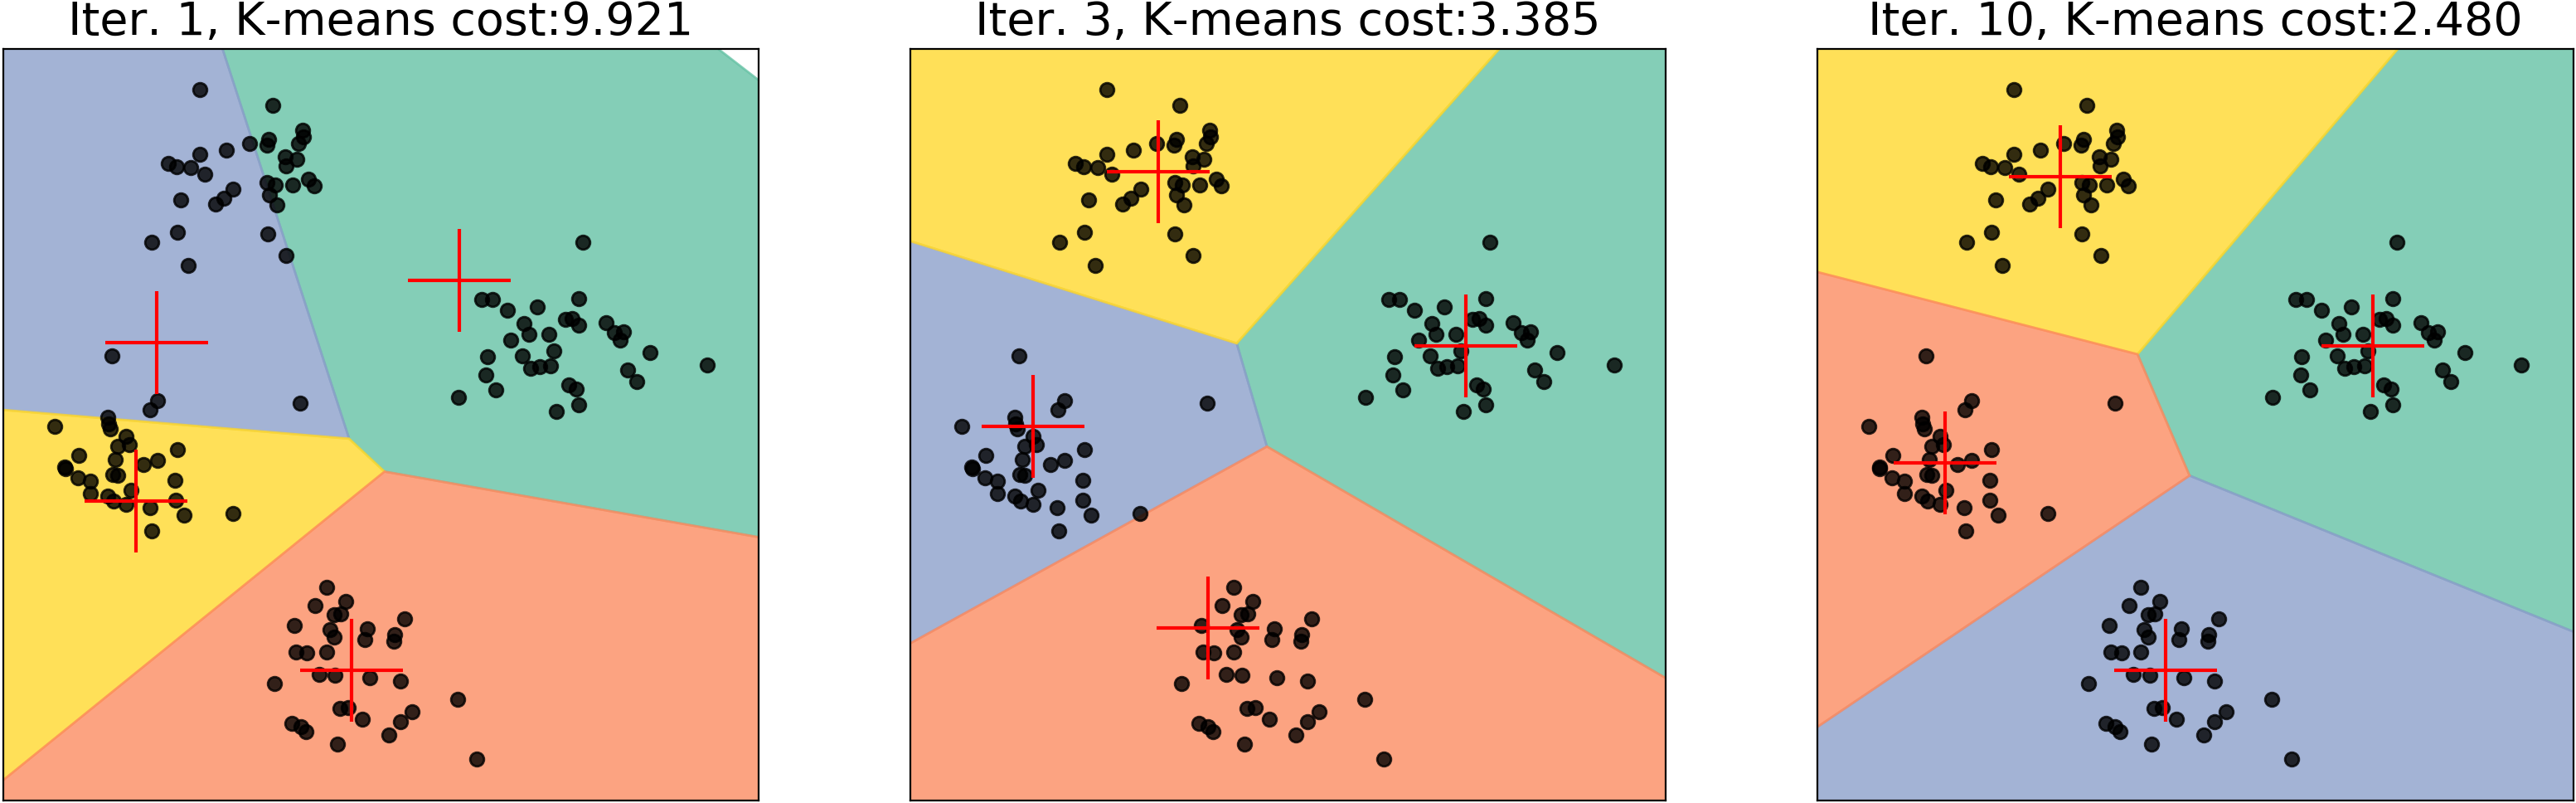
\includegraphics[scale=0.35]{TeX_files/voronoi_kmeans.png}
 \caption{Llyod's algorithm with random initialization centers and final Voronoi partitions at different steps: with 1 iteration (left), 3  (middle) and 10 (right) iterations (the algorithm converged). $K$-means costs are given on top.}
 \label{voronoi_graph}
 \end{figure}
\begin{figure}[h]
\begin{center}
\mybox{
\begin{minipage}{0.85\linewidth}
\begin{algorithmic}%[1]\tt
\small
\STATE {\bfseries Input:} N points $\bx_1,\ldots,\bx_n\in\RR^p$ and the number of clusters $K$.
\STATE {\bfseries Output:} Cluster centers $\hat\bc_1,\dots,\hat\bc_K$ and clusters assignments.
\STATE {\bfseries Init:} Set $\mathcal{L}_{\textnormal{old}}=\infty.$ and chose $K$ seed points $\bc_1,\dots,\bc_K$. Compute the $K$-means cost $\mathcal{L}_{\textnormal{curr}}$ given in \cref{kmeans_min_problem} with these points as centers.
\WHILE{$\mathcal{L}_{\textnormal{curr}}  < \mathcal{L}_{\textnormal{old}}$} 
\STATE{\tt 1: }Compute the Voronoi partitioning of the data with $\bc_1,\dots,\bc_K$ as centers. Get $K$ clusters, $C_1,\dots,C_K$.
\STATE{\tt 2: }On each clusters, compute the sample means $\hat\bc_1,\dots,\hat\bc_K$:
\begin{equation}
  \hat\bc_i = \frac{1}{|C_i|}\sum_{x_j\in C_i} x_j
\end{equation}
\STATE{\tt 3: }Set $\mathcal{L}_{\textnormal{old}} = \mathcal{L}_{\textnormal{curr}}$ and compute the new $K$-means cost $\mathcal{L}_{\textnormal{curr}}$ with $\hat\bc_1,\dots,\hat\bc_K$ as centers.
\ENDWHILE
\end{algorithmic}
\end{minipage}
}
   \caption{$K$-means Lloyd's algorithm}
   \label{algo:lloyd_algo}
\end{center}
\vspace{-15pt}
\end{figure}
 Note that Lloyd's algorithm has several drawbacks: 
\begin{enumerate}
\item It is a hard-assignment method since it assigns points to clusters and does not reflect a level of uncertainty on the assignments such as a probability of belonging to a cluster.
 \item The number of clusters has to be given, we will see some techniques to select the number of clusters in \cref{estim_nb_clusters_sect}.
 \item The worst-case time complexity $T(n)$ is superpolynomial, $T(n)=2^{\Omega(\sqrt{n})}$ iterations \citep{kmeans_slow_arthur_2016} (not bounded above by any polynomial). Fortunately, in practice it is observed that Lloyd's algorithm converges quickly to a local minimum.
 \item If the initial centers are chosen randomly, the resulting $K$-means cost can be made arbitrarily bad compared to the optimal clustering (see section 5.2 of \citep{hennig2015handbook}). $K$-means$++$ \citep{Arthur:2007:KAC:1283383.1283494} address this problem by choosing carefully the initializations centers in Lloyd's algorithm, see \Cref{algo:kmeans++_algo} for the procedure, and showed that $K$-means$++$ is a $\log K$ approximation algorithm for the $K$-means objective, see \Cref{kmeans++_theo}.
\begin{theorem}{\citep{Arthur:2007:KAC:1283383.1283494}}
\label{kmeans++_theo}
Let $S$ be the set of centers output by the algorithm $K$-means$++$ and $\mathcal{L}(S)$ be the $K$-means cost of the clustering obtained using $S$ as the centers. Then $\EE[\mathcal{L(S)}]\leq O(\log(K))\mathcal{L}^*$, where $\mathcal{L}^*$ is the cost of the optimal $K$-means solution. 
\end{theorem}
\item $K$-means can not distinguish noise or select relevant features. This last point is particularly important in the case of high dimensional data, since it is generally accepted that the most relevant clusters lies in subspaces of much smaller dimension, we will discuss this phenomenon in \cref{curse_dim_section}. An idea would be to adapt Lloyd's method to the weighted $p^{th}$-root of the Minkowski metric
\begin{equation}
  d_{\bw}(\bx,\by) = \sum_{l=1}^p w_l|\bx_l - \by_l|^p,
\end{equation}
with $\bw$ a weight vector updated at each iterations. A first method of weighted $K$-means has been introduced in \citep{makarenkov2001optimal} and further developed in \citep{Huang_mink_kmeans} ($WK$-Means) for the Euclidean norm. An extension to the Minkowski metric is proposed in \citep{CordeirodeAmorim:2012:MMF:2051369.2051484} ($MWK$-Means) that outperforms $K$-means and $WK$-Means. Note that the use of a different metric has a profound impact on the implementation and running costs since the computation of Minkowski centers is not straightforward.
\end{enumerate}
\begin{figure}[h]
\begin{center}
\mybox{
\begin{minipage}{0.85\linewidth}
\begin{algorithmic}%[1]\tt
\small
\STATE {\bfseries Input:} N points $\bx_1,\ldots,\bx_n\in\RR^p$ and the number of clusters $K$.
\STATE {\bfseries Init:} Chose one center $\bc_1$ uniformly at random among the data points and add it to the set $\mathcal{S}$.
\FOR{$j=2$ to $K$ } 
\STATE{\tt 1:} Chose a point $\bx$ with probability proportional to $\min_{\bc \in \mathcal{S}} d(\bx,\bc)^2$  and add it to $\mathcal{S}$.
\ENDFOR
\STATE {\tt 2:} Proceed with $K$-means algorithm and the set $\mathcal{S}$ as initialization clusters. 
\end{algorithmic}
\end{minipage}
}
   \caption{$K$-means$++$ algorithm}
   \label{algo:kmeans++_algo}
\end{center}
\vspace{-15pt}
\end{figure}
The research on $K$-means is dense and several variants of this method has been developed. For instance $K$-medoids \citep{KaufmanR90} uses points of the data as centers, Mini-batch $K$-means\citep{Sculley:2010:WKC:1772690.1772862} takes mini-batches of data to reduce significantly computational times without penalizing too much the $K$-means cost or clustering algorithms that enjoy strong theoretical guarantees on non-worst case scenarios using notion of stability\citep{Ostrovsky2006}. The reader can refer to \citep{hennig2015handbook} for further details on this topic.
\subsection{Agglomerative Hierarchical Methods}
In this section, we will present the Agglomerative Hierarchical clustering, a very popular method due to its simplicity and the resulting nested structure of clusters that it produces. The idea of Hierarchical clustering is to form a hierarchy of clusters (i.e. nested clusters) according to a merging rule which helps us to see how clusters are related to each other (a structure unavailable with $K$-means). There exists two types of hierarchical clustering: agglomerative and divisive. The first type consists to start from $N$ sets, each containing one element of the dataset and merge sets iteratively into larger groups according to an agglomeration rule and a similarity, i.e. building a hierarchy, until finding only one cluster that contains the whole data. The similarity can be a Minkowski distance, the cosine similarity or other distance such as Hamming, Hellinger or Mahalanobis.  The divisive procedure is the opposite of the agglomerative, starting from the whole dataset and splitting iteratively until obtaining $N$ sets. Divisive methods are generally very expensive, with a complexity of $O(2^n)$ \citep{Guenoche1991} , and are therefore not used in practice. 
Let us consider the agglomerative procedure and a metric $d$, a simple implementation is to build the dissimilarity matrix of the $N$ original clusters $\{\bx_1\},\dots,\{\bx_N\}$ noted $S=(d_{ij}=d(i,j))_{i,j\in [N]^2}$ (which is symmetric) and consider the couple $(i,j)$ such that $d_{ij}$ is the smallest dissimilarity in $S$. We create a new cluster $i \cup j$, add it to the matrix $S$ with the rule $d_{i\cup j, k}=\min\{d_{ik},d_{jk}\}$ and remove the rows and columns of sets $i$ and $j$ in $S$. The iteration of this procedure leads to one final cluster containing all points in the dataset. This method is called `Single-linkage' clustering \citep{Graham:1985:HMS:1435654.1436662} and a naive implementation is given in \Cref{algo:single_linkage_hier_algo} with a complexity of $O(n^3)$. Note that it can be optimized to $O(n^2)$\citep{hierarchicalMurtagh}. The hierarchy can be visualized via a binary tree called `dendrogram' in \Cref{dendrogram_graph}. This method has a severe drawback called `chaining phenomenon' where clusters can be merged due to close points even if it contains other points very distant. A alternative method called `Complete-linkage' clustering solves this problem by taking the maximum instead of the minimum in step 1 of the single-linkage algorithm in \Cref{algo:single_linkage_hier_algo}. Similarly to Single-linkage method, the complexity of the naive method is $O(n^3)$ but can be optimized to $O(n^2)$. Another popular method worth mentioning for its use of cluster centers is the Ward's method\citep{ward63} also called Ward's minimum variance method which consists to optimize an objective function, generally the sum of squares. Let us consider the merging cost of combining clusters $A$ and $B$:
\begin{align*}
  \Delta(A,B) &= \sum_{i\in A\cup B} \|\bx_i - \bc_{A \cup B} \|^2-\sum_{i\in A} \|\bx_i - \bc_{A} \|^2-\sum_{i\in B} \|\bx_i - \bc_{B} \|^2\\
  &= \frac{n_An_B}{n_A+ n_B}\|\bc_A - \bc_B \|^2,
\end{align*}
where $\bc_i$ and $n_i$ are the center of cluster $i$ and its size respectively.  This quantity is positive, hence the within-group variance increases when merging two clusters. Ward's method seek to minimize this growth. Alternatively, this leads to achieve the maximum between-cluster variance. 

We can notice that agglomerative methods differ on the computation of dissimilarities following the agglomeration process (step 2 in \cref{algo:single_linkage_hier_algo}). Lance and Williams developed an updating formula \citep{lance_williams_67} for these dissimilarities that generalize several agglomerative methods. The dissimilarity between a new merged cluster $i \cup j$ and cluster $k$ is
\begin{equation}
  d(i \cup j,k) = \alpha_i d(i,k)+\alpha_jd(j,k)+\beta d(i, j) +\gamma |d(i,k)-d(j,k)|,
\end{equation}
where the parameters $\alpha_i , \alpha_j, \beta, \gamma$ depend on the clustering criterion. For instance, the single-linkage method is recovered by setting $\alpha_i =\alpha_j = 1/2$, $\beta =0$ and $\gamma =-1/2$, the complete-linkage method with $\alpha_i =\alpha_j = 1/2$, $\beta =0$ and $\gamma =1/2$ and Ward's method can be expressed in this framework \citep{Batagelj88generalizedward,f.1985multidimensional,jambu1989exploration} with $\alpha_i=(n_i+n_k)/(n_i+n_j+n_k)$, $\alpha_j=(n_j+n_k)/(n_i+n_j+n_k)$, $\beta=-n_k/(n_i+n_j+n_k)$ and $\gamma=0$. The reader can find parameters for other methods in Table 6.1 of \citep{hennig2015handbook}.
 \begin{figure}[h]
 \center
 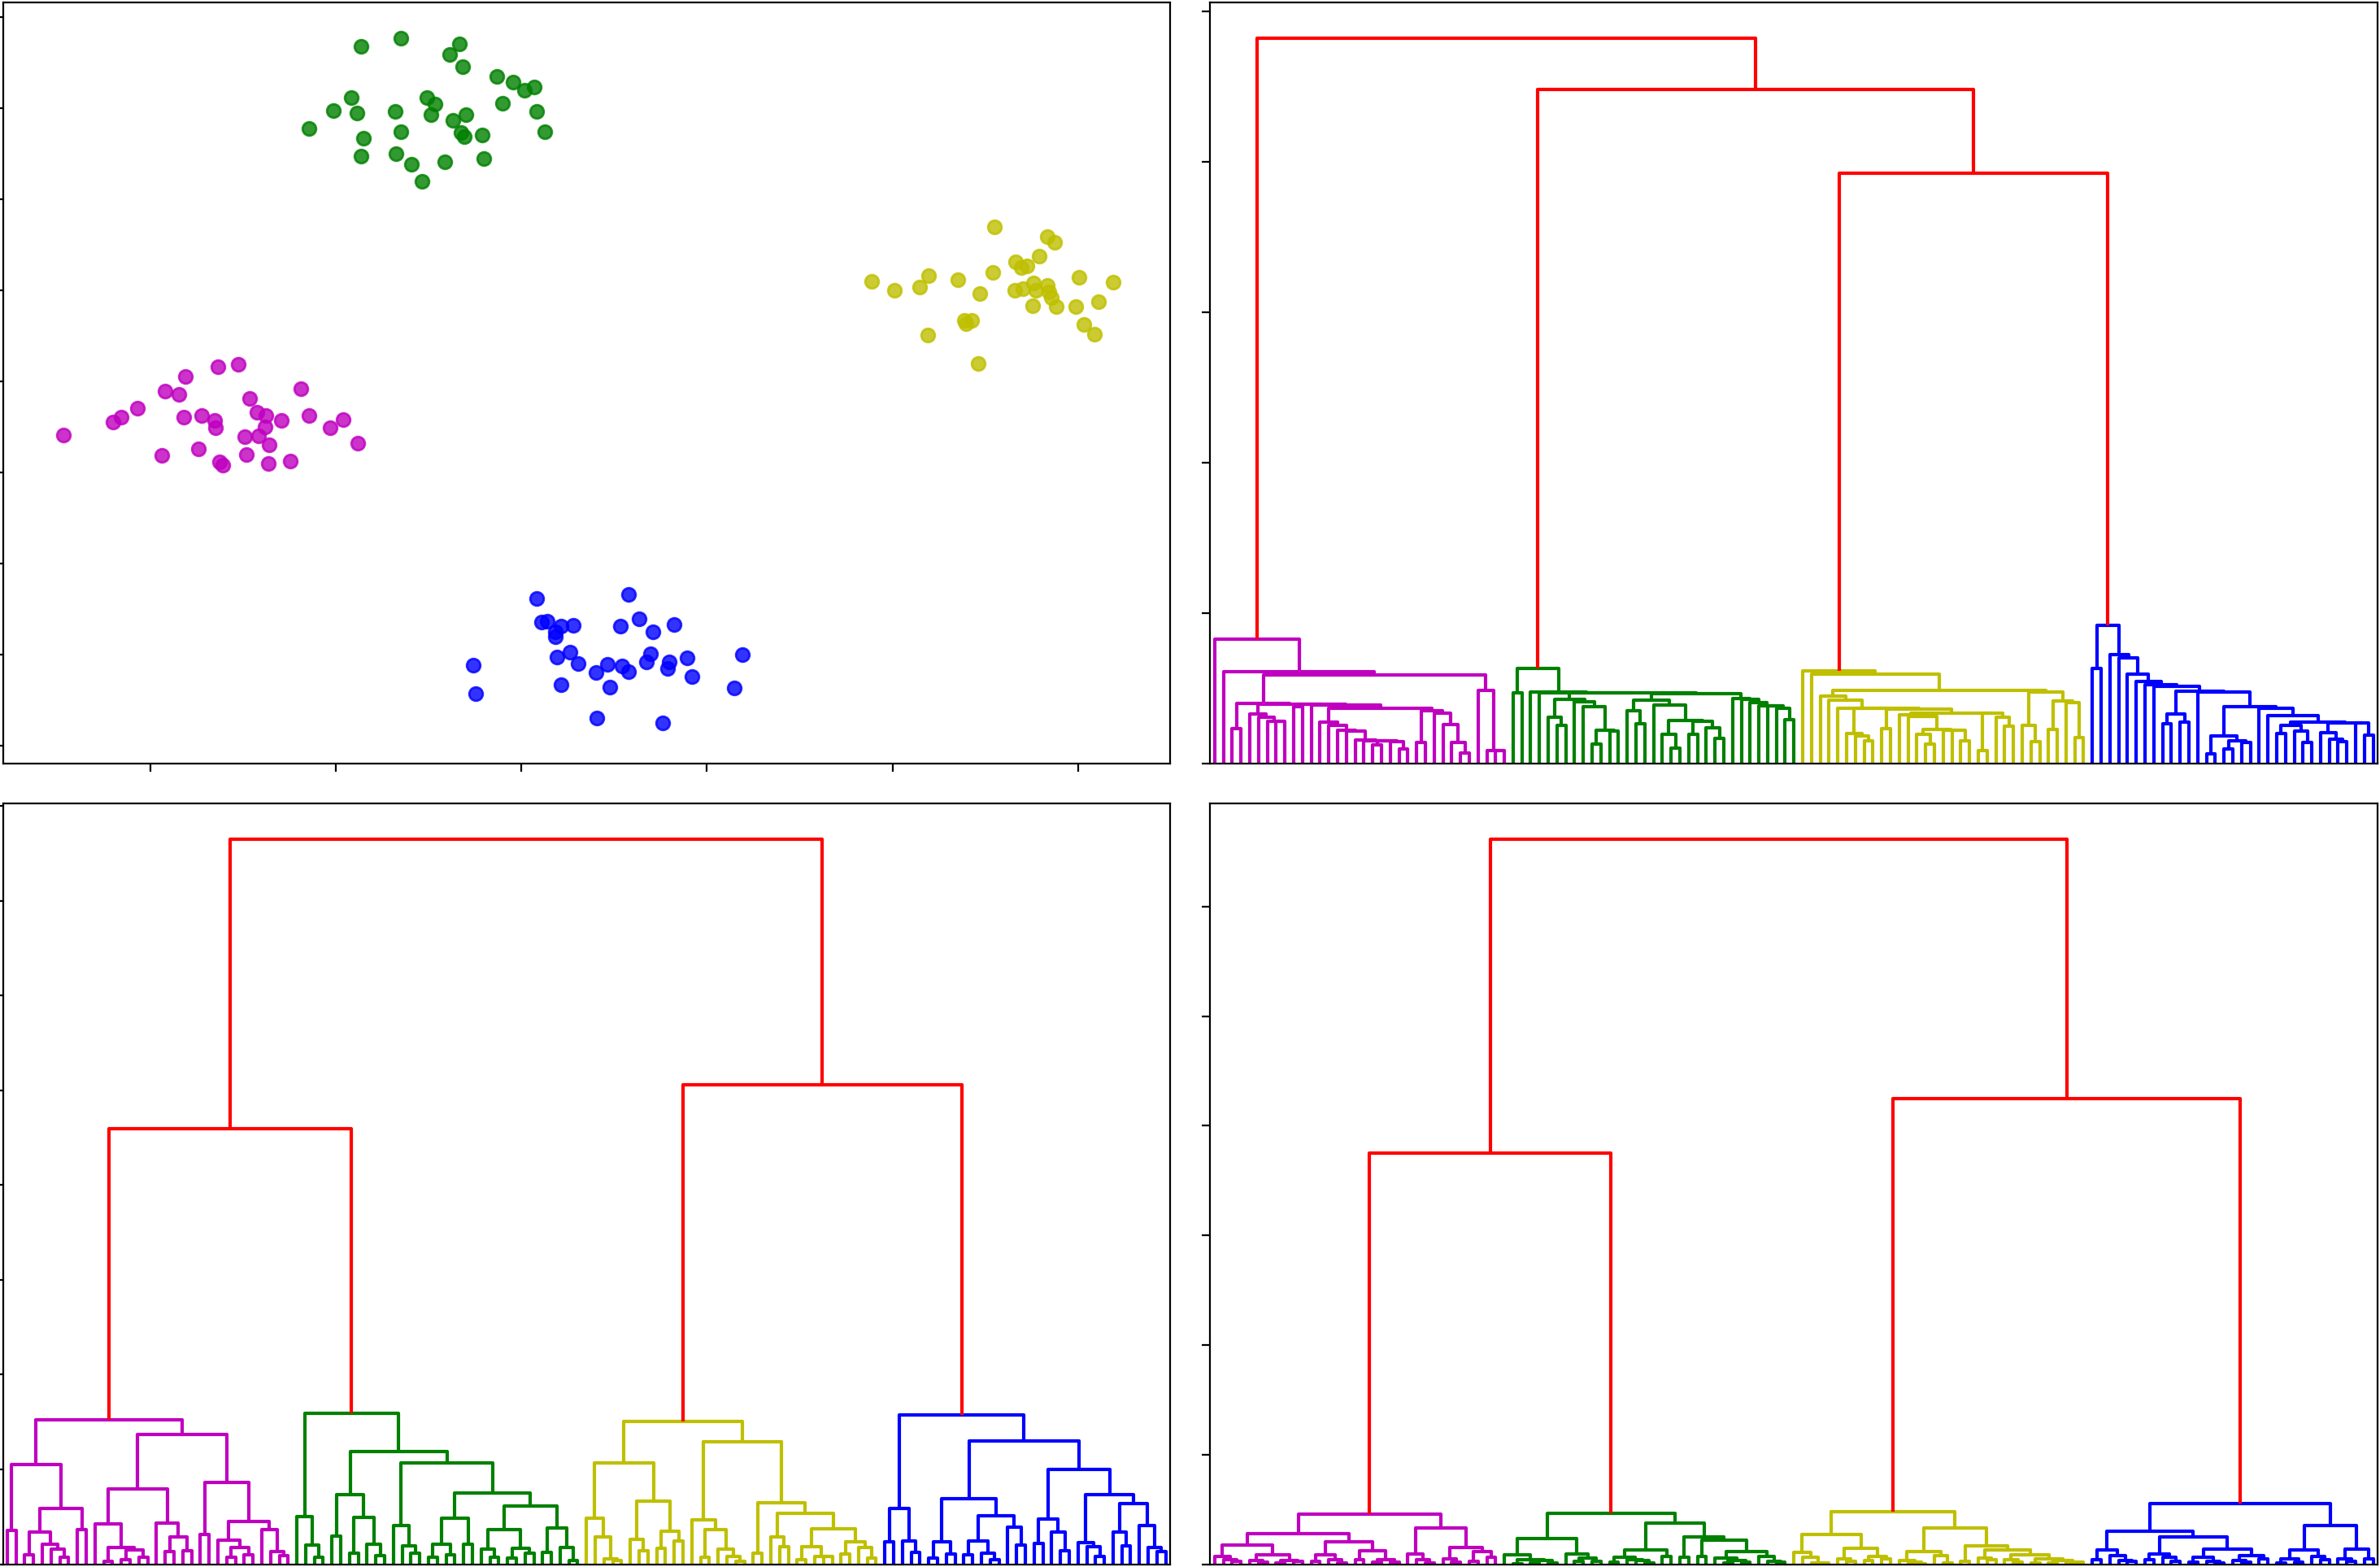
\includegraphics[scale=0.35]{TeX_files/dendrogram.png}
 \caption{A dataset with 4 clusters (top-left) used with the Agglomerative hierarchical clustering and its corresponding dendrogram, single-link (top-right), complete-link (bottom-left) and Ward's method (bottom-right). A simple way for finding clusters would be to cut the dendrogram with a horizontal line from bottom to top until finding the number of clusters desired. Note the difficulty to select the 4 original clusters.}
 \label{dendrogram_graph}
 \end{figure}
 More efficient algorithms relies on `Nearest Neighbor Chains'. The reader can refer to \citep{hierarchicalMurtagh} for a detailed review on Agglomerative hierarchical methods.

\begin{figure}[h]
\begin{center}
\mybox{
\begin{minipage}{0.85\linewidth}
\begin{algorithmic}%[1]\tt
\small
\STATE {\bfseries Input:} A dissimilarity matrix $S$.
\WHILE{at least 2 objects remain in S} 
\STATE{\tt 1:} Determine the smallest dissimilarity $d_{ij}$ in $S$.
\STATE{\tt 2:} Let $m$ be the size of $S$, compute the dissimilarities for the new cluster $i\cup j$:
\begin{equation}
  d_{i\cup j, k} = \min\{d_{ik},d_{jk}\},\quad k\in [m], m\neq i,j.
\end{equation}
\STATE{\tt 3:} Add the dissimilarities of $i\cup j$ in $S$ and remove those of clusters $i$ and $j$.
\ENDWHILE
\end{algorithmic}
\end{minipage}
}
   \caption{Simple single-linkage hierarchical clustering}
   \label{algo:single_linkage_hier_algo}
\end{center}
\vspace{-15pt}
\end{figure}
\subsection{Spectral clustering}
Recently, spectral clustering has become widely used thanks to its performance compared to traditional clustering techniques and it's computational attractiveness. One interesting feature of spectral clustering is that it does not make any assumptions on the form of the clusters contrary to $K$-means. This method of clustering relies deeply on the graph theory \citep{Donath:1973:LBP:1664638.1664644,Fiedler1973}. The reader can refer to \citep{Luxburg:2007:TSC:1288822.1288832} and \citep{SPIELMAN2007284} for a study of the literature on this topic. Although several methods exists which all refer to the term `Spectral clustering' we will address the simplest formulation of this method. Let us consider $\bx_1,\dots,\bx_N$, $N$ points in $\RR^p$ and a similarity measure $s_{ij} \geq 0$ between $\bx_i$ and $\bx_j$. We can construct the similarity matrix $\bS=(s_{ij})_{i,j\in [N^2]}$ which can be represented by a similarity graph $G=(V,E)$ where the vertices set $v_1,\dots,v_N$ correspond to the points $\bx_1,\dots,\bx_N$ and the edge between $v_i$ and $v_j$ exists if $s_{ij}\neq 0 $ and hence has weight $s_{ij}$. Note that $G$ is an undirected graph, i.e. $s_{ij}=s_{ji}$. The main idea of spectral clustering is to find a partition of $G$ with minimal cuts, that is find a partition such that the edges between different group has low weight and those within a group have high weight. This can be done by analyzing the spectrum of the Laplacian matrix $\bL$ of $\bS$ and a clustering such as $K$-means in a low-dimensional subspace spanned by relevant eigenvectors of $\bL$. It is clear that a sparse graph $G$ is interesting for such cutting problem. There exists several methods to sparsify $\bS$: \todos{changer en $W$}
\begin{description}
\item[$K$-nearest neighbor graphs:] Modify the similarity matrix $\bS$ by keeping for each nodes the $k$-nearest neighbors and set $s_{ij}=0$ for the other vertices. We can make this graph undirected in different ways, see section 2.2 of \citep{Luxburg:2007:TSC:1288822.1288832}.
\item[$\varepsilon$-neighborhood graph:] We connect nodes $v_i$ and $v_j$ if $d(\bx_i,\bx_j)\leq \varepsilon$, this graph is usually unweighted.
\item[Fully connect graph:] Used with a similarity function such as Gaussian $s_{ij}=\exp(-\|\bx_i-\bx_j\|^2/2\sigma^2)$. $\sigma$ has a similar role to $\varepsilon$ in the $\varepsilon$-neighborhood graph.
\end{description}
We will note $\bW$ the resulting weighted adjacency matrix. The reader can find more details and behavior of these different graph in section 8 of \citep{Luxburg:2007:TSC:1288822.1288832}. The most simple approach for spectral clustering is to consider the `unnormalized graph Laplacian', $\bL=\bD-\bW$, where $\bD$ is a diagonal matrix called the `degree matrix' and the element $i$ of its diagonal is the degree of the vertex $v_i$, $d_i= \sum_{j=1}^Ns_{ij}$. An important property of this matrix is that its smallest eigenvalue is 0 and its corresponding eigenvector is the constant one vector (see proposition 1 of \citep{Luxburg:2007:TSC:1288822.1288832}). For the following, we say that $A \subset G$ is connected if any two vertices in $A$ can be joined with a path where the intermediate vertices lies in A. $A$ is a connected component if it is connected and there are no connections between $A$ and $\bar A$. An important result for spectral clustering is the following proposition:
\begin{proposition}[Number of connected components, proposition 2 in \citep{Luxburg:2007:TSC:1288822.1288832}]
 The multiplicity $k$ of the eigenvalue 0 of $\bL$ is the number of connected components $A_1,\dots,A_k$ in the graph $G$. The eigenspace of eigenvalue 0 is spanned by the indicator vectors $1_{A_1},\dots,1_{A_k}$ of these components.
 \end{proposition}
 The most simple implementation of the spectral clustering is given in \Cref{algo:unnorm_spectr_alg}
 \begin{figure}[h]
\begin{center}
\mybox{
\begin{minipage}{0.85\linewidth}
\begin{algorithmic}%[1]\tt
\small
\STATE {\bfseries Input:} A similarity matrix $\bS\in \RR^{N\times N}$ and the number of clusters to find $k$.
\STATE {\bfseries Output:} Clusters $A_1,\dots,A_k$.
\STATE{\tt 1:} Construct the weighted adjacency matrix $\bW$.
\STATE{\tt 2:} Compute the unnormalized Laplacian $\bL$.
\STATE{\tt 3:} Compute the $k$ eigenvectors $\bv_1,\dots,\bv_k$ of $\bL$ corresponding to the $k$ smallest eigenvalues of $\bL$.
\STATE{\tt 4:} Let $\bV\in \RR^{N\times k}$ be the matrix containing the vectors  $\bv_1,\dots,\bv_k$  as columns.
\STATE{\tt 5:} For $i \in [N]$, let $\by_i \in \RR^k$ be the vector corresponding to the $i^{th}$ row of $\bV$.
\STATE{\tt 6:} Cluster the points $(\by_i)_{i\in[N]} \in \RR^k$ with the $k$-means algorithm into clusters $C_1,\dots,C_k$.
\STATE{\tt 7:} Construct clusters $A_1,\dots,A_k$ with $A_i=\{i, \by_i \in C_i\}$
\end{algorithmic}
\end{minipage}
}
   \caption{Unnormalized spectral clustering according to \citep{Luxburg:2007:TSC:1288822.1288832}}
   \label{algo:unnorm_spectr_alg}
\end{center}
\vspace{-15pt}
\end{figure}
Two other types of Laplacian matrices are used in the literature called `normalized graph Laplacians' and offer theoretical advantages compared to the unnormalized Laplacian (see section 8.4 of \citep{Luxburg:2007:TSC:1288822.1288832}). They are defined as following:
\begin{equation}
  \bL_{\textnormal{sym}} = \bI - \bD^{-\nicefrac{1}{2}}\bW\bD^{\nicefrac{1}{2}} \quad \textnormal{and} \quad \bL_{\textnormal{rw}}= \bI-\bD^{-1}\bW.
\end{equation}
We will refrain from addressing these two matrices, we shall content ourselves with saying that there exists more efficient spectral clustering algorithms called `Normalized spectral clustering' that are in the same spirit as \Cref{algo:unnorm_spectr_alg}, the reader can refer to \citep{Shi:2000:NCI:351581.351611,Ng01onspectral,Luxburg:2007:TSC:1288822.1288832} for a deeper analysis of the use of this Laplacians. We will simply give an insight on the mechanics behind the spectral clustering algorithm and we shall study the problem from a graph point of view. The spectral algorithm is an approximation to the problem of partitioning the graph $G$. For $A$ and $B$, two disjoint subsets of $G$ we define
\begin{equation}
  cut(A,B)=\sum_{i\in A, j\in B} w_{ij}.
\end{equation}\todos{voir si ne pas noter sij}
Two common objective function to minimize for such partitioning are RatioCut \citep{Hegen1992} and Ncut \citep{Shi:2000:NCI:351581.351611} defined as 
\begin{align*}
&\textnormal{RatioCut}(A_1,\dots,A_k)=\sum_{i=1}^k\frac{cut(A_i,\bar A_i)}{|A_i|},\\
&\textnormal{Ncut}(A_1,\dots,A_k)=\sum_{i=1}^k\frac{cut(A_i,\bar A_i)}{\textnormal{vol}(A_i)},
\end{align*}
where $|A|$ is the number of vertices in $A$ and $\textnormal{vol}(A) = \sum_{i\in A}d_i$. Note that these two objective functions try to achieve a "balanced" partitioning, a small component leads to a high value of these objective functions. Unfortunately, such partition problem is NP-hard \citep{Wagner1993,Luxburg:2007:TSC:1288822.1288832}. Hopefully a relaxation of this problem with RatioCut is:
\begin{equation}
\label{relaxed_ratiocut_pb}
  \min_{\bH\in{\RR^{N\times K}}} Tr(\bH^T\bL\bH)\quad \textnormal{subject to}\quad \bH^T\bH = \bI.
\end{equation}
It turns out that choosing $\bH$ as the matrix with the first $k$ eigenvectors of $\bL$ as columns is a solution of \Cref{relaxed_ratiocut_pb} (see 5.2 of \citep{Luxburg:2007:TSC:1288822.1288832}) which is exactly the step 4 in \Cref{algo:unnorm_spectr_alg}. The same relaxation can be done for the Ncut objective function
\begin{equation}
  \min_{\bU\in\RR^{N\times k}} Tr(\bU^T\bD^{-\nicefrac{1}{2}}\bL\bD^{-\nicefrac{1}{2}}\bU)\quad \textnormal{subject to}\quad \bU^T\bU = \bI.
\end{equation}
These relaxation does not give guarantees on the quality of the solutions and the resulting partition can be arbitrary worse than the optimal one in regards to RatioCut and Ncut \citep{Guattery98,Nadler07fundamentallimitations}. In particular, spectral clustering methods are global methods and fail to identify clusters at different scales \citep{Nadler07fundamentallimitations}. But these approximations are computationally attractive and very simple to solve, especially with a sparse weighted adjacency matrix. Usually, it is preferred to use $\bL_{\textnormal{rw}}$ and the normalized spectral clustering method.
\subsection{Finding the number of clusters}
The determination of the number of clusters in a dataset is fundamental and still unsolved problem. Numerous approaches to this problem has been developed over the years, see \citep{Hardy:1996:NC:255810.255820,Milligan1985} and Chapter 26 of \citep{hennig2015handbook}. Several popular heuristics relies on a graphical interpretation of the quality of clustering. The most popular are the Elbow criterion which consists to perform clusterings with different number of clusters $K$ and compute the ratio of the between group variance versus the total variance (the F-test statistic) for each of them. The detection of an `elbow' indicates the appropriate number of clusters i.e. with larger $K$, the clusters does not give more information on the variance. Another technique that relies on a graphical interpretation is the Silhouette method \citep{Rousseeuw:1987:SGA:38768.38772} which asses how well a point is assigned to its cluster compared to nearest neighbor cluster. A more formal approach is the `Gap Statistic' developed in \citep{gap_stat_tibsh_2001}, an efficient statistical procedure that compare the change in within-cluster dispersion with that expected under a reference null distribution. In the case of the spectral clustering, one can use the `eigengap' heuristic on the eigenvalues $\lambda_1,\dots,\lambda_N$ of the Laplacian matrix by choosing $K$ such that $\lambda_1,\dots,\lambda_K$ are small and $\lambda_{K+1}$ is relatively large (see section 8.3 of \citep{Luxburg:2007:TSC:1288822.1288832}). Finally, a model selection criterion widely used on probabilistic models and important in our work is the Bayesian Information Criterion (BIC). This method has been developed in \citep{schwarz1978} following the work of Akaike on the AIC \citep{Akaike1998}. The idea of this method under the assumption that the observations $\{\bx_i,\dots,\bx_N\}$ are drawn from an exponential family is to derive from the approximation of the asymptotic expansion of the Bayes estimator the following quantity
\begin{equation}
  \textnormal{BIC} = \hat\ell_j(\hat\theta,\bx)-\frac{1}{2}k_j\log(N),
\end{equation}
where $\hat\ell_j(\hat\theta,\bx)$ is the maximized likelihood of model $j$, $\hat\theta$ is the MLE and $k_j$ is number of free parameters of model $j$. Therefore, the model selection rule is to chose the model for which the BIC is the largest. BIC has several nice properties, it penalizes the complexity of the model which is interesting since choosing the model only on the criterion of the{} likelihood in the case of Gaussian mixtures leads to select as many components as there are points. One can remark that all procedures mentioned previously require to perform a large number of clusterings and select the best model according to those criteria. This approach is computationally expensive. In \Cref{sparse_weight_vect_estim}, we try to address this challenge by iteratively penalizing the weight vector of large Gaussian mixture in an EM-like procedure.
\section{The Gaussian Mixture Model}
We will now focus on the main tool of this thesis. The Gaussian Mixture Model (GMM) is an important framework for clustering problems. Unlike the other methods previously seen, it is a probabilistic approach for clustering. One of the main advantages of model-based clustering is that the resulting partition can be interpreted statistically. It assumes that the observations are drawn from a
mixture distribution the components of which are Gaussian  with parameters $(\bmu_k,\bSigma_k)$:
\begin{equation}
\varphi_{\bmu_k,\bSigma_k}(x)=\frac{1}{(2\pi)^{p/2}|\bSigma_k|^{1/2}} \exp\Big(-\frac{1}{2}(\bx-\bmu_k)^\top\bSigma_k^{-1}(\bx-\bmu_k)\Big)
\end{equation}
Let $\btheta$ be the list containing all the unknown parameters of a Gaussian mixture model: the family of means $\bmu = (\bmu_1,\ldots,\bmu_K)
\in (\RR^p)^K$, the family of covariance matrices $\bSigma = (\bSigma_1,\ldots,\bSigma_k)\in(\mathcal S_{++}^p)^K$ and the vector of cluster probabilities  $\bpi=(\pi_1,\ldots,\pi_k)\in [0,1]^K$ such that $\b1_p^\top\bpi=1$.
The density of one observation $\bX_1$ is then given by:
\begin{equation}\label{mixture}
p_{\btheta}(\bx)=\sum_{k=1}^K\pi_k\varphi_{\bmu_k,\bSigma_k}(\bx),\qquad \forall \bx\in\RR^p,
\end{equation}
where $\btheta=(\bmu,\bSigma,\bpi)$.
This model can be interpreted from a latent variable perspective. Let $Z$ be a discrete random variable
taking its values in the set $[K]$ and such that $\Pb(Z=k) = \pi_k$ for every $k\in[K]$. The random variable $Z$
indicates the cluster from which the observation $\bX$ is drawn.  Considering that all the conditional distributions
$\bX|Z=k$ are Gaussian, we get the following formula for the marginal density of $X$:
\begin{equation}
p_{\btheta}(\bx)=\sum_{k=1}^K \Pb(Z=k)p_{\theta}(\bx|Z=k) = \sum_{k=1}^K\pi_k\varphi_{\bmu_k,\bSigma_k}(\bx),\qquad \forall \bx\in\RR^p.
\end{equation}
In the clustering problem, the goal is to assign $X$ to a cluster or, equivalently, to predict the cluster $Z$ of the vector $\bX$.
A prediction function in such a context is $g:\RR^p\to[K]$ such that $g(\bX)$ is as close as possible to $Z$. If we measure the
risk of a prediction function $g$ in terms of misclassification error rate $R_\btheta(g) = \Pb_\btheta(g(\bX)\not=Z)$, then it is
well known that the optimal (Bayes) predictor $g^*_\btheta \in \arg\min_g R_\btheta(g)$ is provided by the rule
$$
g^*_\btheta(\bx) = \arg\max_{k\in [K]} \tau_k(\bx,\btheta),
$$
where $\tau_k(\bx,\btheta)=p_{\btheta}(Z=k|\bX=\bx)$ stands for the conditional probability of the latent variable $Z$ given $\bX$.
In the Gaussian mixture model, Bayes's rule implies that
\begin{equation}
\label{tau_bayes}
\tau_k(\bx,\btheta)=\frac{p_{\btheta}(\bx|Z=k)\Pb(Z=k)}{p_{\btheta}(\bx)}
=\frac{\pi_k\varphi_{\bmu_k,\bSigma_k}(\bx)}{\sum_{k'=1}^K\pi_{k'}\varphi_{\bmu_{k'},\bSigma_{k'}}(\bx)}
\end{equation}
Since the true value of the parameter $\btheta$ is not available, formula (\ref{tau_bayes}) can not be
directly used for solving the problem of clustering. Instead, a natural strategy is to estimate $\btheta$
by some vector $\hat\btheta$, based on a sample $\bX_1,\ldots,\bX_n$ drawn from the density $p_\btheta$, and
then to define the clustering rule by
\begin{equation}
\label{gen_clust}
\hat g(\bx) = g^*_{\hat\btheta}(\bx)=\arg\max_{k\in [K]} \tau_k(\bx,\hat\btheta)=\arg\max_{k\in [K]}\
\hat\pi_k\varphi_{\hat\bmu_k,\hat\bSigma_k}(\bx).
\end{equation}
A common approach to estimating the parameter $\btheta$ is to rely on the likelihood maximization. Let $\bX_1,\dots,\bX_n$ with $\bX_i\in \RR^p$ be a set of iid observations drawn from the density $p_{\btheta}$
given by (\ref{mixture}). The following graphical model depicts the scheme of the observations:
%%GRAPH of pgm
\begin{figure}[h]
\centering\small
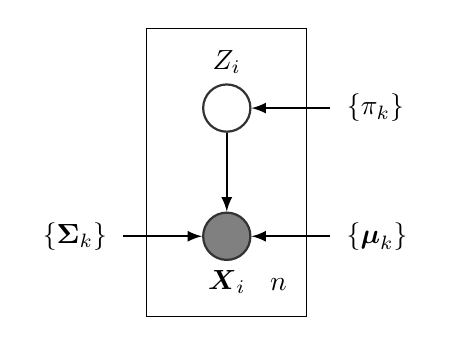
\begin{tikzpicture}
\tikzstyle{main}=[circle, minimum size = 6mm, thick, draw =black!80, node distance = 10mm]
\tikzstyle{connect}=[-latex, thick]
\tikzstyle{box}=[rectangle, draw=black!100]
  \node[main, fill = black!50] (x) [label=below:{$\bX_i$}] { };
  \node[main] (z) [above=of x,label=above:{$Z_i$}] {};
  \path (z) edge [connect] (x);
  \node[rectangle, inner sep=7mm,draw=black!100, fit= (z) (x)] {};
\node[rectangle, below=of x, inner sep=-10mm, fit= (z) (x),label=below right:{$n$}, xshift=4mm,yshift=-2mm] {};
\node[main,draw=none] (a) [right=of x] {$\{\bmu_k\}$};
\path (a) edge [connect] (x);
\node[main,draw=none] (b) [left=of x] {$\{\bSigma_k\}$};
\path (b) edge [connect] (x);
\node[main,draw=none] (c) [right=of z] {$\{\pi_k\}$};
\path (c) edge [connect] (z);
\end{tikzpicture}
\end{figure}
The log-likelihood of the Gaussian mixture model is
\begin{equation}\label{log-likelihood}
\ell_n(\btheta)=\sum_{i=1}^{n}\log{p_{\btheta}(\bx_i)}=
\sum_{i=1}^{n}\log\bigg\{{\sum_{k=1}^K\pi_k\varphi_{(\bmu_{k},\bSigma_{k})}(\bx_i)}\bigg\}.
\end{equation}
Because of the presence in this equation of the logarithm of a sum, the maximization of the log-likelihood is
a difficult nonlinear and nonconvex problem. In particular, this is not a exponential family distribution yielding simple expressions.
A commonly used approach for approximately maximizing (\ref{log-likelihood}) with respect to $\btheta$ is the Expectation-Maximization
(EM) Algorithm \citep{dempster77} that we recall below.

Summarizing the content of this section, we can describe the following  natural approach to solving the clustering problem under Gaussian
mixture modeling assumption:
\begin{figure}[h]
\begin{center}
\mybox{
\begin{minipage}{0.95\linewidth}
\begin{algorithmic}%[1]\tt
\small
\STATE {\bfseries Input:} data vectors $\bx_1,\ldots,\bx_n\in\RR^p$ and the number of clusters $K$
\STATE {\bfseries Output:} function  $\hat g : \RR^p\to [K]$
\STATE {\tt 1:} Estimate $\btheta=(\bpi,\bmu,\bSigma)$ by maximizing the log-likelihood:
\begin{align}\label{step:1}
\hat\btheta
    &\in\arg\max_{\btheta\in\bTheta}  \ell(\btheta|\bx_1,\dots,\bx_n)
    =\arg\max_{\bpi,\bmu,\bSigma}  \sum_{i=1}^{n}\log\bigg\{{\sum_{k=1}^K\pi_k\varphi_{\bmu_{k},\bSigma_{k}}(\bx_i)}\bigg\}.
\end{align}
\STATE {\tt 2:} Output the clustering rule:
\begin{equation}
\label{step:2}
\hat g(\cdot) = \arg\max_{k\in [K]} \hat\pi_k\varphi_{\hat\bmu_k,\hat\bSigma_k}(\cdot).
\end{equation}
\end{algorithmic}
\end{minipage}
}
   \caption{Clustering under Gaussian mixture modeling}
   \label{algo:general}
\end{center}
\vspace{-15pt}
\end{figure}
\subsection{EM Algorithm}
The goal of the EM algorithm is to approximate a solution of the problem \eqref{step:1}.
Since this optimization problem contains a nonconvex cost function, it is impossible to
design a polynomial time algorithm that provably converges to the global maximum point. Instead,
the EM algorithm provides a sequence $\{\hat\btheta(t)\}_{t\in\NN}$ of parameter values such that
the cost function (\textit{i.e.}, the log-likelihood) evaluated at these values forms an
increasing sequence that converges to a local maximum.

The main idea underlying the EM algorithm is the following representation of the log-likelihood
of one observation derived from the log-sum inequality:
\begin{equation}\label{hint}
\log\bigg\{{\sum_{k=1}^K\pi_k\varphi_{\bmu_{k},\bSigma_{k}}(\bx_i)}\bigg\} =
\max_{\substack{\btau\in[0,1]^K \ \btau^\top \b1_K=1}} \sum_{k=1}^K \Big\{\tau_{k}\log\varphi_{\bmu_{k},\bSigma_{k}}(\bx_i)+\tau_{k} \log(\pi_k/\tau_{k})\Big\}.
\end{equation}
Let us denote by $\bTau = (\tau_{i,k})$ a $n\times K$ matrix with nonnegative entries such that $\bTau\b1_K = \b1_n$, that is each
row of $\bTau$ is a probability distribution on $[K]$. Combining \eqref{step:1} and \eqref{hint}, we get
\begin{align}\label{eq:3}
\hat\btheta
    &\in\argmax_{\btheta=(\bpi,\bmu,\bSigma)}\max_{\bTau}
    \sum_{i=1}^{N} \sum_{k=1}^K \Big\{\tau_{i,k}\log\varphi_{\bmu_{k},\bSigma_{k}}(\bx_i)+\tau_{i,k}
    \log(\pi_k/\tau_{i,k})\Big\}.
\end{align}
The great advantage of this new representation of the log-likelihood function is that the cost
function in \eqref{eq:3}, considered as a function of $\btheta$ and $\bTau$, is biconcave, \textit{i.e.},
it is concave with respect to $\btheta$ for every fixed $\bTau$ and concave with respect to $\bTau$ for
every fixed $\btheta$. In such a situation, one can apply the alternating maximization approach to sequentially
improve on an initial point. In the present context, an additional attractive feature of the cost function
in \eqref{eq:3} is that the two optimization problems involved in the alternating maximization procedure
admit explicit solutions.
\begin{figure}[ht]
\begin{center}
\mybox{
\begin{minipage}{0.85\linewidth}
\begin{algorithmic}%[1]\tt
%\SetLine%\SetAlgoLined
\small
\STATE {\bfseries Input:} data vectors $\bx_1,\ldots,\bx_n\in\RR^p$ and the number of clusters $K$
\STATE {\bfseries Output:} parameter estimate $\hat\btheta = \{\hat\bmu_k,\hat\bSigma_k,\pi_k\}_{k\in[K]}$
\STATE {\tt 1:} Initialize $t=0$, $\btheta=\btheta^0$.
\STATE {\tt 2:} {\bf Repeat}
\STATE \qquad {\tt 3:} Update the parameter $\bTau$:
\begin{align*}
\tau_{i,k}^{t}  &= \frac{\pi_k^{t}\varphi_{\bmu_k^{t},\bSigma_k^{t}}(\bx_i)}{\sum_{k'\in[K]}\pi^{t}_{k'}\varphi_{\bmu^{t}_{k'},\bSigma^{t}_{k'}}(\bx_i)}.
\end{align*}
\STATE \qquad{\tt 4:} Update the parameter $\btheta$:
\begin{align*}
\pi_k^{t+1}     &= \frac1n\sum_{i=1}^n \tau_{i,k}^t,\qquad
\bmu_k^{t+1}    = \frac1{n\pi_k^{t+1}}\sum_{i=1}^n \tau_{i,k}^t\bx_i,\\
\bSigma_k^{t+1} &= \frac1{n\pi_k^{t+1}}\sum_{i=1}^n \tau_{i,k}^t(\bx_i-\bmu_k^{t+1})(\bx_i-\bmu_k^{t+1})^\top.
\end{align*}
\STATE \qquad {\tt 5:} increment $t$: $t=t+1$.
\STATE {\tt 6:} {\bf Until} stopping rule.
\STATE {\tt 7:} {\bf Return} $\btheta^{t}$.
\end{algorithmic}
\end{minipage}}
   \caption{EM algorithm for Gaussian mixtures}
   \label{algo:EM}
\end{center}
\end{figure}
\begin{lem}
\label{lemma1}
Let us introduce the cost function
\begin{equation}
F(\btheta,\bTau) = \sum_{i=1}^{n} \sum_{k=1}^K \Big\{\tau_{i,k}\log\varphi_{\bmu_{k},\bSigma_{k}}(\bx_i)+\tau_{i,k}
    \log(\pi_k/\tau_{i,k})\Big\}.
\end{equation}
Then, the following two optimization problems
\begin{align}
\hat\btheta(\bTau)&\in \arg\max_{\btheta} F(\btheta,\bTau),\qquad \hat\bTau(\btheta)\in \arg\max_{\bTau} F(\btheta,\bTau)
\end{align}
has explicit solutions given by
\begin{align}
\label{em-sols}
\hat\pi_k     &= \frac1n\sum_{i=1}^n \tau_{i,k},\qquad\hat\bmu_k = \frac1{n\hat\pi_k}\sum_{i=1}^n \tau_{i,k}\bx_i ,\qquad \forall k\in[K],\\
\hat\bSigma_k &= \frac1{n\hat\pi_k}\sum_{i=1}^n \tau_{i,k}(\bx_i-\hat\bmu_k)(\bx_i-\hat\bmu_k)^\top,\qquad\forall k\in[K],\\
\hat\tau_{i,k}&= \frac{\pi_k\varphi_{\bmu_k,\bSigma_k}(\bx_i)}{\sum_{k'\in[K]}\pi_{k'}\varphi_{\bmu_{k'},\bSigma_{k'}}(\bx_i)},\qquad\forall k\in[K],\ \forall i\in[n] \label{tau_ik_em}.
\end{align}
\end{lem}
Based on this result, the EM algorithm is defined as in Figure~\ref{algo:EM}.
The algorithm operates iteratively and needs a criterion to determine when
the iterations should be stopped. There is no clear consensus on this point in the
statistical literature, but it is a commonly used  practice to stop when one of the
following conditions is fulfilled:
\begin{description}
\item[i)]  The number of iterations $t$ exceeds a pre-specified level $t_{\max}$.
\item[ii)] The increase of the log-likelihood over past $t_0$ iterations is not
significantly different from zero: $\ell_n(\btheta^{t})-\ell_n(\btheta^{t-t_0})\le \varepsilon$
for some pre-specified values $t_0\in\NN$ and $\varepsilon>0$.
\end{description}
EM is conceptually easy and each iteration increases the log-likelihood:
$$
\ell_n(\btheta^{t+1})\ge \ell_n(\btheta^{t}),\qquad \forall t\in\NN.
$$
The complexity at each step of the EM algorithm is $O(Knp^2)$ and
it usually requires many iterations to converge. In a high-dimensional setting
when $p$ is large, the quadratic dependence on $p$ may result in prohibitively
large running times. However, the computation of the elements of the covariance
matrices $\bSigma^t_k$ and the mean vectors $\bmu^t_k$ can be parallelized which
may lead to considerable savings in the running time.
\subsection{$K$-means from the EM angle}

In this section, we will see that the $K$-means problem is closely related to the EM algorithm. We rewrite the minimization problem of $K$-means defined in \cref{kmeans_min_problem} as following
\begin{equation}
  \min_{\bc_1,\dots,\bc_K}\min_{\bR \in \{0,1\}^{N\times K}}\sum_{i=1}^N\sum_{k=1}^K r_{ik}\|\bx_i - \bc_k \|^2,
\end{equation}
where the matrix $\bR$ follows the $1$-of-$K$ coding scheme, i.e. if a point $\bx_i$ is assigned to the cluster $m$, then $r_{im}=1$ and $r_{il}=0, \forall l\in [K] \neq m$. One can see the underlying iterative procedure, the first one consists to minimize the objective function with respect to $\bc_1,\dots,\bc_K$ with $\bR$ fixed (Maximization step) and the second one consists to minimize the objective function with respect to $\bR$ with $\bc_1,\dots,\bc_K$ fixed (Expectation step). Consider the \textbf{E}-step, the objective function is linear with respect to $\bR$.  It consists for a data point $\bx_i$, to find the cluster $k$ such that $k = \argmin_{j\in[K]}\|\bx_i-\bc_j\|^2$. For the \textbf{M}-step, setting the gradient with respect to $\bc_k$ to 0 gives us
\begin{equation}
  2\sum_{i=1}^N r_{ik} (\bx_i-\bc_k) = 0,
\end{equation}
which leads to
\begin{equation}
  \bc_k = \frac{\sum_{i=1}^N r_{ik}\bx_i}{\sum_{i=1}^N r_{ik}}.
\end{equation}
Since $\sum_{i=1}^Nr_{ik}$ is the size of the cluster $k$, we recovered the Lloyd's algorithm.
\section{The curse of dimensionality}
\label{curse_dim_section}
The expression `Curse of dimensionality' introduced by R.Bellman in his book on dynamic programming \citep{Bellman:1957} refers to the problems linked with high dimension. One can see that evaluating a function on the segment $(0,1)$ with a step size of $0.1$ is straightforward. However, evaluating the function in a grid of dimension 10 requires $10^{10}$ computations which can be intractable even today within a reasonable time. Many computational and statistical problems arise in this setting. Sometimes the literature refers to a `high dimensional' setting when $p \gg n$ and more precisely when the model considered has more parameters or degree of freedom than there are observations. In the following, we recall some classical phenomenons that appear in this context and focus on the clustering with high dimensional data. 

We saw previously different clustering methods that rely on a distance such as the Euclidean distance. It turns out that in a high dimensional setting, the notion of nearest point vanishes: the minimal distance increases but on the other hand the variance of the distance between points has a slower increase. Consider 2 $p$-dimensional random variables $\bX,\bX'$ and the Euclidean norm, the scaled deviation is then
\begin{equation}
  \frac{\textnormal{sdev}[\|\bX-\bX'\|^2]}{\EE[\|\bX-\bX'\|^2]} \approx \frac{1}{\sqrt{p}},
\end{equation}
and goes to $0$ when $p\rightarrow\infty$. A direct consequence of such distance concentration phenomenon is the loss of relevance of the methods based on discriminating near and far neighbors such as those studied in the previous section (nearest center for $K$-means, agglomeration in hierarchical clustering or constructing adjacency graph for spectral clustering). In the clustering context, a strong assumption for ensuring the separation of clusters would be to consider the inter-cluster distance dominant compared to the variance within each clusters. Another phenomenon is the "error accumulation", consider the classical linear regression setting  $\bY=\bX\bbeta^*+\beps$ with $\bX\in \RR^{N\times p}$ and $\beps_1,\dots,\beps_N$ i.i.d. centered with variance $\sigma^2$. The least-square estimator $\hat\bbeta = \argmin_{\bbeta\in\RR^{p}}\|\bY-\bX\bbeta\|^2$ verify the following estimation error
\begin{equation}
  \EE[\|\hat\beta-\bbeta^*\|^2]=p\sigma^2.
\end{equation}
Therefore we can see that the estimation error increases linearly with the dimension. Furthermore, an interesting phenomenon that occurs in high dimension is that spaces are mostly empty and the realizations of a $p$-dimensional random vector with a uniform probability distribution on the unit hypersphere lies with high probability close to the boundary of this hypersphere. Therefore, the data belong mostly in a $p-1$ dimensional subspace. Interestingly, the ratio of the volume of a hypersphere versus the volume of the hypercube goes to 0 as $p\rightarrow\infty$ (see section 2.3 of \citep{Zimek2012}). This means that most of the volume lies in the corner of the hypercube. Therefore, any methods based on a spherical distance such as the Euclidean norm is meaningless in this context. One could consider a probabilistic approach to overcome the issues with high dimension. Unfortunately, model-based clustering suffers over-parametrization. In the Gaussian mixture model of $K$ components in dimension $p$, the number of free parameters to estimate is
\begin{equation}
   \nu = \underbrace{(K-1)}_\text{Weights}+ \underbrace{Kp}_\text{Means} + \underbrace{Kp(p-1)^2}_\text{Covariances Matrices},
 \end{equation}
which for $p=10$ and $K=5$ is 4104. Moreover, the evaluation of $\hat\tau_{i,k}$ in \cref{tau_ik_em} needs to evaluate the inverse of the covariance matrix $\hat\bSigma_k$ which is called the precision matrix. If $n<<\nu$ the matrices $\hat\bSigma_k$ with $ k\in[K]$ are ill conditioned and the precision matrices are prone to large numerical errors or more often are singular and the problem can not be solved.

Several popular methods are used to overcome these issues. One can reasonably consider that multiple variables are correlated or that most of the dimensions are irrelevant and therefore clusters may live on a lower-dimensional subspace. A first approach would be to perform a dimension reduction like Principal Component Analysis (PCA) but this leads to a decoupling of the dimension reduction task from the clustering task and may lead to a poor selection of the subspace \citep{bouveyron:hal-00750909}, keeping information from irrelevant dimensions. Moreover, the interpretation of the resulting linearly transformed dimensions are difficult to interpret. Another approach called `feature selection' consists to select the most relevant features but fails when clusters live in different subspaces. This scenario leads to the development of `subspace clustering' techniques that goes one step further by selecting the most relevant features for each clusters separately (see \citep{Parsons:2004:SCH:1007730.1007731} for a review on this topic). 

In our work, we will focus in the regularization technique and make sparse assumption on the structure of the Gaussian mixture model. The goal is to reduce the number of free parameters and tackle the problem of estimating the inverse of the covariance matrix. In \cref{chapgraphlasso}, we tackle this challenge by studying some nice structural properties of precision matrices.

The reader can find a more thorough study of high dimensional statistics in \cite{giraud2014introduction,Zimek2012}. For an overview of clustering in high dimension see \citep{bouveyron:hal-00750909,Parsons:2004:SCH:1007730.1007731}.
\section{Some contributions}
In this section, we present some works carried out during this thesis which have unfortunately not been able to be the subject of an in-depth study that can be published. The first part deals with the sparse hypothesis of the precision matrices within a high dimensional Gaussian mixture and adapts the single-component Graphical Lasso from \citep{glasso07} to the mixture setting. In the second part, we assume that the weight vector of the mixture is sparse in order to obtain an estimator of the number of components in the mixture that is generally unknown. 
\subsection{Graphical Lasso for Gaussian mixtures}\label{chapgraphlasso}
As we saw in the introduction chapter\todos{changer en section}, the number of free parameters in a full GMM with $K$ components in dimension $p$ are $(K-1)+Kp+Kp(p+1)/2$ which means that for $K=5$ and $p=100$ we have $125704$ parameters to estimate. In this high dimensional setting, the EM algorithm experiences severe performance degradation. In particular, the inversion of the covariance matrices are challenged. One way to tackle these problems is to use regularization. We will make the assumption on some structure on the inverse of the covariance matrix of a component called the precision or concentration matrix. The work presented in this chapter is inspired by \citep{glasso07}, \citep{banerjee}, \citep{yuanLin_graph} and \citep{meinshausen2006} in which they penalize the components of the precision matrix of a Gaussian graphical model. We generalize this work to the Gaussian mixture model.

\subsubsection{Introduction}
We consider $\bX=(\bX^{(1)},\dots,\bX^{(p)})$ a random vector admitting a $p$-dimensional normal distribution $\mathcal N(\bmu, \bSigma)$ with $\bSigma$ non-singular. One can construct an undirected graph $G=(V,E)$ with $p$ vertices corresponding to each coordinates and, $E=(e_{i,j})_{1\leq i < j \leq p}$, the edges between the vertices describing the conditional independence relationship among $\bX^{(1)},\dots,\bX^{(p)}$. 
If in this graph, $e_{i,j}$ is absent in $E$ if and only if $X^{(i)}$ and $X^{(j)}$ 
are independent conditionally to the other variables $\{X^{(l)}\}$ with $l\neq i,j$ (noted $X^{(i)} \ci X^{(j)}|X^{(l)}\, l\neq i,j$), then $G$ is called the Gaussian concentration graph model for the Gaussian random vector $\bX$. 
This property is particularly interesting in the study of the inverse of the covariance matrix. Let us denote $\bSigma^{-1}=\bOmega=(\omega_{i,j})$ the precision matrix. The components of this matrix verify $\omega_{i,j}=0$ if and only if $X^{(i)} \ci X^{(j)}$ conditionally to the other variables. We recall in the following lemma this well known result

\begin{lemma}[Conditional independence in Gaussian concentration graph model]
Consider $\bX=(\bX^{(1)},\dots,\bX^{(p)})$ a p-dimensional random vector with a multivariate normal distribution $\mathcal N(\bmu, \bSigma)$, note $\bSigma^{-1}=\bOmega=(\omega_{i,j})$, then $X^{(i)} \ci X^{(j)}|X^{(l)} \iff \omega_{i,j}=0$ with $l\neq i,j$ 
\end{lemma}
\begin{proof}
This result can be found in \citep{edwards2000introduction}, consider the density of $\bX$
\begin{equation}
  \varphi_{\bmu,\bSigma}(\bx)=\frac{1}{(2\pi)^{p/2}|\bSigma|^{1/2}} \exp\Big(-\frac{1}{2}(\bx-\bmu)^\top\bSigma^{-1}(\bx-\bmu)\Big),
\end{equation}
it can be rewritten as
\begin{equation}
  \varphi_{\bmu,\bSigma}(\bx) = \exp(\alpha + \beta^T\bx-\frac{1}{2}\bx^T\bOmega\bx),
\end{equation}
with $\beta=\bOmega\bmu$ and $\alpha=\frac{1}{2}\log(|\bOmega|)-\frac{1}{2}\bmu^T\bOmega\bmu-\frac{p}{2}\log(2\pi)$. Then, the previous equation can be rewritten as 
\begin{equation}
\label{exp_fam_cond_ind}
  \exp\big(\alpha + \sum_{j=1}^p\beta_j\bx^{(j)}-\frac{1}{2}\sum_{j=1}^p\sum_{(i=1)}^p\omega_{i,j}\bx^{(j)}\bx^{(i)}\big).
\end{equation}
Now, for $X,Y,Z$ three random variables, we have $X \ci Y|Z$ iff the joint density can be factorized into two factors $f_{X,Y,Z}(x,y,z)=h(x,z)g(y,z)$ with $h$ anf $g$ two functions. Then, at the light of  \cref{exp_fam_cond_ind}, we have $X^{(i)}\ci X^{(j)}|X^{(l)} \iff \omega_{i,j}=0$.
\end{proof}
The literature on this subject focused on a first hand on the estimation of the graph structure, \citep{dempster1972cov_select} developed a greedy forward or backward search method to estimate the set of non-zero components in the concentration matrix. The forward method relies on initializing an empty set and select iteratively an edge with an MLE fit for $\mathcal{O}(p^2)$ different parameters. The procedure stops according to a suitable selection criterion. The backward method performs in the same manner by starting with all edges and performing deletions. It is obvious that such methods are computationally intractable in high dimension. In \citep{meinshausen2006}, the authors studied a neighborhood selection procedure with lasso. The goal is to estimate the neighborhood $ne_{X^{(i)}}$ of a node $X^{(i)}$ which is the smallest subset of $G\setminus\{X^{(i)}\}$ such that $X^{(i)} \ci \big\{X^{(j)}: X^{(j)}\in G\setminus\{ne_{X^{(i)}}\}\big\} | X_{ne_{X^{(i)}}}$. The estimation of the neighborhood is cast as a regression problem with a lasso penalization. The authors showed that this procedure is consistent for sparse high dimensional graphs and computationally efficient. More precisely, let $\theta^{(i)} \in \RR ^p$ be the vector of coefficient of the optimal prediction,\todos{banerjee p488, consistency lies on choice of penalty}
\begin{equation}
  \theta^{(i)} = \argmin_{\theta:\theta_i=0}\EE\Big[ X^{(i)}-\sum_{k=1}^p\theta_k X^{(k)}\Big],
\end{equation}
then the components of $\theta^{(i)}$ are determined by the precision matrix, $\theta^{(i)}_j=-\omega_{i,j}/\omega_{i,i}$. Therefore, the set of neighbors of $X^{(i)}\in G$ is given by
\begin{equation}
  ne_{X^{(i)}}= \{X^{(j)}, j\in[p]: \omega_{i,j} \neq 0 \}.
\end{equation}
Now, let $\XX$ be the $n\times p$-dimensional matrix such that the column $\XX^{(i)}$ is the $n$ observations vector of $X^{(i)}$, given a regularization parameter $\lambda \geq 0$ carefully chosen, the Lasso estimate $\hat\theta^{i,\lambda}$ of $\theta^{(i)}$ is given by
\begin{equation}
  \hat\theta^{i,\lambda} = \argmin_{\theta:\theta_i=0}\Big(\frac{1}{n}\|\XX^{(i)}-\XX\theta \|_2^2 + \lambda\|\theta\|_1 \Big).
\end{equation}
The authors proved under several assumptions that 
\begin{equation}
  P(\hat{ne}_{X^{(i)}}^{\lambda}=ne_{X^{(i)}})\rightarrow 1 \quad \text{for}\, n\rightarrow \infty,
\end{equation}
and for some $\epsilon > 0$,
\begin{equation}
  P(\hat E^{\lambda}=E)=1-\mathcal{O}(\exp(-cn^{\epsilon}))\quad \text{for}\, n\rightarrow \infty.
\end{equation}
Therefore, this method recovers the conditional independence structure of sparse high-dimensional Gaussian concentration graph \todos{ajouter un mot sur la complexité} at exponential rates. However, this method performs model selection but does not estimate the parameters of the model. One  could estimate the parameters of a model which has been selected by this method. Such procedure often leads to instability of the estimator since small changes on the data would change the model selected \citep{yuanLin_graph}, \citep{breiman1996}. One major difficulty of a method that would perform both tasks is to ensure that the estimator of the precision matrix is positive definite. \citep{yuanLin_graph} proposed a penalized-likelihood method that performs model selection and parameter estimation simultaneously as well as ensuring the positive definiteness of the precision matrix. Their approach is similar to \citep{meinshausen2006} as they use the $\ell_1$ penalty but with the likelihood and the addition of a positive definite constraint. The log-likelihood for $\bOmega$ based on a  centered random sample $\bX_1,\dots,\bX_n$ of $\bX$ is
\begin{equation}
  \frac{n}{2}\log(|\bOmega|) - \frac{1}{2}\sum_{i=1}^n\bX_i^T\bOmega\bX_i
\end{equation}
and the constrained minimization problem over the set of positive definite matrices is
\begin{equation}
\label{prec_matrix_gauss_min_pb}
  \text{min}\Big\{-\log(|\bOmega|) + \frac{1}{n}\sum_{i=1}^n\bX_i^T\bOmega\bX_i\Big\} \quad \text{subject to}\quad \sum_{i\neq j} |\omega_{i,j}|\leq t,
\end{equation}
with $t\geq 0$ a tuning parameter. Note that $\hat\bmu=\bar\bX$. Consider the empirical covariance matrix $\bS=1/n\sum_{i=1}^n\bX_i^T\bX_i$, the \cref{prec_matrix_gauss_min_pb} can be rewritten as 
\begin{equation}
  \text{min}\Big\{-\log(|\bOmega|) + \text{tr}(\bS\bOmega)\Big\} \quad \text{subject to}\quad \sum_{i\neq j} |\omega_{i,j}|\leq t.
\end{equation}
Since the whole problem is convex, the Lagrangian form is given by
\begin{equation}
\label{yuan_lkhood_pb}
  \mathcal L (\lambda, \bOmega) = -\log(|\bOmega|) + \text{tr}(\bS\bOmega) + \lambda\sum_{i\neq j} |\omega_{i,j}|,
\end{equation}
with $\lambda$ the tuning parameter. A non-negative garrote-type estimator is provided in \citep{yuanLin_graph} but can be only applied when a good estimator of $\bOmega$ is available\todos{regarder de plus pres}. Therefore, we will continue our study of the Lasso-type estimator, the authors provided an asymptotic result
\begin{theorem}[Theorem 1 from \citep{yuanLin_graph}]
If $\sqrt{n}\lambda \rightarrow \lambda_0\geq0$  as $n\rightarrow\infty$, the lasso-type estimator is such that 
\begin{equation*}
  \sqrt{n}(\hat\bOmega-\bOmega)\rightarrow\argmin_{\bU=\bU^T}(V),
\end{equation*}
in distribution where
\begin{equation*}
  V(\bU)=\textnormal{tr}(\bU \bSigma \bU \bSigma)+\textnormal{tr}(\bU \bW)+\lambda_0\sum_{i\neq j}\big\{ u_{i,j}\textnormal{sign}(\omega_{i,j})I(\omega_{i,j}\neq 0)+|u_{i,j}|I(\omega_{i,j} =0) \big\}
\end{equation*}
in which $\bW$ is a random symmetric $p\times p$ matrix such that $\textnormal{vec}(\bW) \sim \mathcal N (0, \Lambda)$, and  $\Lambda$ is such that
\begin{equation*}
  \textnormal{cov}(w_{i,j},w_{i',j'}) = \textnormal{cov}(X^{(i)}X^{(j)},X^{(i')}X^{(j')}).
\end{equation*}
\end{theorem}\todos{mettre un commentaire sur ce resultat et aspect algorithmique}
Unfortunately, the computational complexity of interior point methods for maximizing \cref{yuan_lkhood_pb} is $\mathcal O (p^6)$ and at each steps, we have to compute and store a Hessian matrix of size $\mathcal O (p^2)$. These prohibitive complexities led the research on more specialized methods. \citep{banerjee} worked on the same approach, solving a maximum likelihood problem with an $\ell_1$ penalty and focusing on the computation complexity by proposing an iterative block coordinate descent algorithm. The problem to maximize is similar to \cref{yuan_lkhood_pb}
\begin{equation}
\label{max_lkhood_gauss_graph}
  \hat\bOmega = \argmax_{\bOmega \succ 0}\{\log(|\bOmega|)-\textnormal{tr}(\bS\bOmega)-\lambda\|\bOmega \|_1\}.
\end{equation}
Note that the $\ell_1$ norm of a matrix $\bOmega$ can be expressed as
\begin{equation}
  \|\bOmega \|_1 = \max_{\| \bU\|_{\infty}\leq 1}\textnormal{tr}(\bOmega\bU),
\end{equation}
injecting this in \cref{max_lkhood_gauss_graph} gives
\begin{equation}
  \max_{\bOmega \succ 0} \min_{\|\bU\|_{\infty}\leq \lambda} \big\{\log(|\bOmega|)-\textnormal{tr}(\bOmega(\bS+\bU))\big\}.
\end{equation}
After exchanging the min and the max, we solve the problem for $\bOmega$ by setting the gradient to $0$ which gives $(\bOmega^{-1})^T-(\bS+\bU)^T=0$ then $\bOmega = (\bS+\bU)^{-1}$. The dual problem is then
\begin{equation}
  \min_{\|\bU \|_{\infty}}\{-\log(|\bS+\bU|) -p\},
\end{equation}
or by setting $\bW = \bS+\bU$,
\begin{equation}
\label{banerjee_min_pb}
  \hat\bSigma = \hat{\bOmega^{-1}}= \argmax \log(|\bW|) \quad \textnormal{s.t}\quad \|\bW-\bS \|_{\infty} \leq \lambda.
\end{equation}
We observe the presence of a log-barrier adding the implicit constraint $(\bS+\bU) \succ 0$. Furthermore, the dual problem estimates the covariance matrix.\todos{pourquoi $\Sigma_{kk}=S_{kk}+\lambda ?$, p488}.\todos{citer les theoremes et choix du param}. To solve this maximization problem, the authors proposed a Block Coordinate Descent Algorithm described in \cref{fig:banerjee_block_algo}. For any symmetric matrix $\bA$, let $\bA_{\setminus k \setminus j}$ be the matrix produced by removing column $k$ and row $j$ to $\bA$. Let $\bA_j$ the $j^{th}$ column of $\bA$ with the element $\bA_{jj}$ removed.
\begin{figure}
\begin{center}
\mybox{
\begin{minipage}{1.1\linewidth}
\begin{algorithmic}[1]%\SetAlgoLined\tt\SetLine
\small
\STATE {\bfseries Input:} Matrix $\bS$, parameter $\lambda$ and threshold $\varepsilon$
\STATE {\bfseries Output:} Estimate of $\bW$
\STATE {{\bf Initialize} $\bW^{(0)} := \bS+\lambda I$}
\REPEAT
\FOR{$j=1,\dots,p$}
\STATE {(a) Let $\bW^{(j-1)}$ denote the current iterate. Solve the quadratic program}
\begin{equation*}
\label{banerjee_algo_min_pb}
  \hat \by := \argmin_{\by}\{\by^T(\bW_{\setminus j \setminus j}^{(j-1)})^{-1}\by:\|\by-\bS_j\|_{\infty}\leq \lambda\}.
\end{equation*}
\STATE {(b) Update the rule: $\bW^{(j)}$ is $\bW^{(j-1)}$ with column/row $\bW_j$ replaced by $\hat\by$.}
\ENDFOR
\STATE{Let $\hat\bW^{(0)}:=\bW^{(p)}$.}
\UNTIL{convergence occurs when
\begin{equation*}
  \textnormal{tr}\big((\hat\bW^{(0)})^{-1}\bS\big) -p +\lambda\big\|(\hat\bW^{(0)})^{-1} \big\|_1\leq \varepsilon.
\end{equation*}
}
\end{algorithmic}
\end{minipage}}
   \caption{Block Coordinate Descent Algorithm}
   \label{fig:banerjee_block_algo}

\end{center}
\end{figure}
They proved that the Block Coordinate Descent algorithm converges, achieving an $\varepsilon$-suboptimal solution to \cref{banerjee_min_pb} and each iterates produce a strictly positive definite matrix. For a fixed number of sweeps $K$, the complexity of this algorithm is $\mathcal O (Kp^4)$. They provide also another algorithm using Nesterov's first order method which has a $\mathcal O(p^{4.5}/\epsilon)$ complexity for $\varepsilon > 0$ the desired accuracy. It is interesting to note that the dual problem of \cref{banerjee_algo_min_pb} in \cref{fig:banerjee_block_algo} is 
\begin{equation}
  \min_{\bx} \bx^T\bW_{\setminus j \setminus j}^{(j-1)}\bx - \bS_j^T\bx + \lambda\|\bx\|_1,
\end{equation}
and strong duality holds, it can best casted as
\begin{equation}
\label{banerjee_dual_lasso}
  \min_{\bx} \|\bQ\bx - \bbb\|_2^2 + \lambda\|\bx\|_1,
\end{equation}
with $\bQ = (\bW_{\setminus j \setminus j}^{(j-1)})^{1/2}$ and $\bbb:=\frac{1}{2}\bQ^{-1}\bS_j$. Therefore, we recover the Lasso problem, more precisely, the algorithm can be interpreted as a sequence of iterative Lasso problems. This approach is similar to another paper that we would like to mention \citep{glasso07}. The authors proposed a faster algorithm based on the Block Coordinate Descent algorithm from \citep{banerjee} called Graphical Lasso. They estimate the matrix $\bW=\bOmega^{-1}$ by performing iterative permutations of the columns of this matrix to make the target column the last for a coupled Lasso problem. The matrices $\bW$ and $\bS$ will be presented as following 
\begin{equation}
\bW =  \begin{bmatrix}
    \bW_{11} & \bw_{12} \\
    \bw_{21} & w_{22}
  \end{bmatrix}, 
  \quad
 \bS =  \begin{bmatrix}
    \bS_{11} & \bs_{12} \\
    \bs_{21} & s_{22}
  \end{bmatrix}, 
\end{equation}
and the Graphical Lasso algorithm is described in \cref{fig:friedman_graph_lasso}. The Lasso problem can be solved via a coordinate descent, the reader can refer to \citep{glasso07} for the procedure. In this problem, the algorithm estimates $\hat\bSigma$ and returns also $\bB = (\bbb^{(1)},\dots,\bbb^{(p)})$, the matrix where each column is the solution of the Lasso problem in \cref{banerjee_dual_lasso} for each column of $\bW$. It is easy to recover $\bOmega$ since 
\begin{equation}
\bW =  \begin{bmatrix}
    \bW_{11} & \bw_{12} \\
    \bw_{21} & w_{22}
  \end{bmatrix}.
  \begin{bmatrix}
    \bOmega_{11} & \bomega_{12} \\
    \bomega_{21} & \omega_{22}
  \end{bmatrix}=
   \begin{bmatrix}
    I_{p-1} & 0 \\
    0 & 1
  \end{bmatrix},
\end{equation}
and
\begin{align*}
  \bomega_{12} &= -\bW_{11}^{-1}\bw_{12}\omega_{22}\\
  \omega_{22} &= 1/(w_{22}-\bw_{12}^T \bW_{11}^{-1}\bw_{12}).
\end{align*}
Therefore, for $j=1,\dots,p$, the permuted target components of $\bOmega$ are
\begin{align*}
  \bomega_{12} &= -\bbb^{(j)}\hat\omega_{22}\\
  \omega_{22} &= 1/(w_{22}-\bw_{12}^T \bbb^{(j)}).
\end{align*}
\begin{figure}
\begin{center}
\mybox{
\begin{minipage}{1.1\linewidth}
\begin{algorithmic}[1]%\SetAlgoLined\tt\SetLine
\small
\STATE {\bfseries Input:} Matrix $\bS$, parameter $\lambda$ and threshold $\varepsilon$
\STATE {\bfseries Output:} Estimate of $\bW$ and $\bB$ a matrix of parameters.
\STATE {{\bf Initialize} $\bW^{(0)} := \bS+\lambda I$ and $\bB=0_{p\times p}$. The diagonal of $\bW$ remained unchanged in what follows.}
\REPEAT
\FOR{$j=1,\dots,p$}
\STATE {(a) Let $\bW^{(j-1)}$ denote the current iterate. Solve the Lasso problem in \cref{banerjee_dual_lasso}
\begin{equation}
  \hat\bx^{(j-1)} = \argmin_{\bx} \frac{1}{2}\|(\bW_{11}^{(j-1)})^{1/2}\bx - \bbb\|_2^2 + \lambda\|\bx\|_1,
 \end{equation}
 with $\bbb:=(\bW_{11}^{(j-1)})^{-1/2}\bs_{12}$.}
\STATE {(b) Update: $\bW^{(j)}$ is $\bW^{(j-1)}$ with $\bw_{12}=\bW_{11}^{(j-1)}\hat\bx^{(j-1)}$. }
\STATE {(c) Save the parameter $\bx^{(j-1)}$ in the $j^{th}$ column of $\bB$.} 
\STATE{(d) Permute the columns and rows of $\bW^{(j-1)}$ such that the $j^{th}$ column is $\bw_{12}$, the next target.}
\ENDFOR
\STATE{Let $\hat\bW^{(0)}:=\bW^{(p)}$.}
\UNTIL{convergence occurs.}
\end{algorithmic}
\end{minipage}}
   \caption{Graphical Lasso}
   \label{fig:friedman_graph_lasso}

\end{center}
\end{figure}
In what follows, we will adapt these methods on a Gaussian mixture models, more precisely we will assume that each clusters present a sparse Gaussian concentration graph. We will rely on the Graphical Lasso for estimating the precision matrix and derive a EM algorithm.
\subsubsection{Graphical Lasso on Gaussian mixtures}
In this section, we present our contribution. We consider a Gaussian mixture model of $K$ components and our task is to estimate the parameters $\btheta=(\theta_1,\dots,\theta_K)$ with $\theta_k=(\pi_k, \bmu_k, \bOmega_k)$ where $\bOmega_k$ is the precision matrix regarding the $k^{th}$ component of the mixture. We denote $\varphi_{(\bmu_{k},\bOmega_{k})}$ the Gaussian density of mean $\bmu_k$ and precision matrix $\bOmega_k$. The penalized log-likelihood is
\begin{equation}
\label{pen-log-likelihood}
\ell_n^{pen}(\btheta)=\sum_{i=1}^{n}\log p_{\btheta}(\bx_i)-pen(\btheta)= \sum_{i=1}^{n}\log \bigg\{ \sum_{k=1}^K\pi_k\varphi_{(\bmu_{k},\bOmega_{k})}(\bx_i)\bigg\} -pen(\btheta).
\end{equation}
We suppose that each component of the mixture has a sparse Gaussian concentration graph. Therefore, in the scope of \citep{banerjee} and \citep{glasso07}, we consider an $\ell_1$ regularization $pen(\theta_k)=\sum_{k=1}^K\lambda_k||\bOmega_k||_{1,1}$ with $\lambda_k >0$. The penalization of the log-likelihood concerns only the precision matrices $\bOmega_k$. Regarding the other parameters $(\pi_k, \bmu_k)$, our algorithm is the same as EM and we can use the same iteration technique as in \cref{lemma1} to maximize the following cost function
\begin{equation}
\label{cost_fun_pen}
F^{pen}(\btheta,\bTau)  = \sum_{k=1}^K \bigg(\sum_{i=1}^{n} \Big\{\tau_{i,k}\log\varphi_{\bmu_{k},\bOmega_{k}}(\bx_i)+\tau_{i,k}
    \log(\pi_k/\tau_{i,k})\Big\}-\lambda_k||\bOmega_k||_{1,1}\bigg).
\end{equation}
The maximization of this function over $\btheta$ and $\bTau$ leads to the two following optimization problems\todos{ajouter les domaines}
\begin{align}
\label{optim-problems}
\hat\btheta(\bTau)&\in \arg\max_{\btheta} F^{pen}(\btheta,\bTau),\qquad \hat\bTau(\btheta)\in \arg\max_{\bTau} F^{pen}(\btheta,\bTau).
\end{align}
For a given $\hat\bTau$, estimates of $(\pi_1,\dots,\pi_K$ and $\bmu_1,\dots,\bmu_K)$ obtained by the first optimization problem in \cref{optim-problems} are the same as in the EM algorithm
\begin{align}
\label{em-sols}
\hat\pi_k     &= \frac1n\sum_{i=1}^n \hat\tau_{i,k},\quad\text{and}\quad\hat\bmu_k = \frac1{n\hat\pi_k}\sum_{i=1}^n \hat\tau_{i,k}\bx_i ,\qquad \forall k\in[K]
\end{align}
And for a given $\hat\btheta$, the estimate of $\bTau$ obtained by the second optimization problem is
\begin{equation}
\label{em-sols-tau}
\hat\tau_{i,k} = \frac{\hat\pi_k\varphi_{\hat\bmu_k,\hat\bOmega_k}(\bx_i)}{\sum_{k'\in[K]}\hat\pi_{k'}\varphi_{\hat\bmu_{k'},\hat\bOmega_{k'}}(\bx_i)}=p_{\btheta}(Z=k|\bX=\bx_i),\qquad\forall k\in[K],\ \forall i\in[n].
\end{equation}
However, due to the penalty $\lambda_k||\bOmega_k||_{1,1}$, the estimation of $\bOmega_k$ is not straightforward.\\
We introduce the weighted empirical covariance matrix
\begin{equation}
\bSigma_{n,k} = \frac{1}{n}\frac{\sum_{i=1}^n\tau_{i,k}(\bx_i-\hat\bmu_k)(\bx_i-\hat\bmu_k)^\top}{\sum_{i=1}^n\tau_{i,k}}
\end{equation}
The Gaussian density in equation \eqref{cost_fun_pen} can be expanded as follows
\begin{align*}
\label{cost_fun_pen_2}
F^{pen}(\btheta,\bTau)  =& \sum_{k=1}^K \bigg( \sum_{i=1}^{n}\Big\{ \tau_{i,k} \Big(
-\frac{p}{2}\log(2\pi)+\frac{1}{2}\log|\bOmega_k|\\
&-\frac{1}{2}(\bx_i-\bmu_k)^T\bOmega_k(\bx_i-\bmu_k) \Big)+\tau_{i,k} \log(\pi_k/\tau_{i,k})\Big\} -\lambda_k||\bOmega_k||_{1,1}\bigg)\\
=& -\frac{np}{2}\log(2\pi)+\sum_{k=1}^K \bigg(\frac{n\pi_k}{2}\log|\bOmega_k|\\
&+\sum_{i=1}^{n}\Big\{ -\frac{\tau_{i,k}}{2}(\bx_i-\bmu_k)^T\bOmega_k(\bx_i-\bmu_k)+\tau_{i,k} \log(\pi_k/\tau_{i,k})\Big\} -\lambda_k||\bOmega_k||_{1,1}\bigg). 
\end{align*}
The opposite minimization problem regarding each $\bOmega_k$ is
\begin{equation}
\bOmega_k \in \argmin_{ \bOmega\succeq 0}\Big\{-\frac{n\pi_k}{2}\log|\bOmega|+\frac{1}{2}\sum_{i=1}^{n}\tau_{i,k}(\bx_i-\bmu_k)^T\bOmega(\bx_i-\bmu_k)+\lambda_k||\bOmega||_{1,1}\Big\}
\end{equation}
Using the well-known commutativity property of the trace operator and dividing by $n\pi_k$
\begin{equation}
\bOmega_k \in \argmin_{ \bOmega\succeq 0} \Big\{ -\frac{1}{2}\log|\bOmega| +\frac{1}{2} tr(\bSigma_{n,k}\bOmega)+\frac{\lambda_k}{n\pi_k}||\bOmega||_{1,1}\Big\}
\end{equation}
At the light of this equation, one can notice that we solves a graphical lasso problem within each cluster. We used a block coordinate ascent algorithm described in \citep{mazum_lasso} to solve this convex problem. The alternating maximization procedure is summarized in \Cref{algo:graph_lasso_EM}.
\begin{figure}
\begin{center}
\mybox{
\begin{minipage}{0.85\linewidth}
\begin{algorithmic}%\SetAlgoLined\tt\SetLine
\small
\STATE {\bfseries Input:} data vectors $\bx_1,\ldots,\bx_n\in\RR^p$ and the number of clusters $K$
\STATE {\bfseries Output:} parameter estimate $\hat\btheta = \{\hat\bmu_k,\hat\bOmega_k,\hat\pi_k\}_{k\in[K]}$
\STATE {\tt 1: Initialize $t=0$, $\btheta=\btheta^0$.}
\STATE {\tt 2: {\bf Repeat}}
\STATE {\tt 3: \qquad Update the parameter $\bTau$:}
\begin{align*}
\tau_{i,k}^{t}  &= \frac{\pi_k^{t}\varphi_{\bmu_k^{t},\bOmega_k^{t}}(\bx_i)}{\sum_{k'\in[K]}\pi^{t}_{k'}\varphi_{\bmu^{t}_{k'},\bOmega^{t}_{k'}}(\bx_i)}.
\end{align*}
\STATE {\tt 4: \qquad Update the parameter $\btheta$:}
\begin{align*}
\pi_k^{t+1}     &= \frac1n\sum_{i=1}^n \tau_{i,k}^t,\qquad \\
\bmu_k^{t+1}    &= \frac1{n\pi_k^{t+1}}\sum_{i=1}^n \tau_{i,k}^t\bx_i\\
\bSigma_{n,k}         &= \frac{1}{n^2\pi_k^{t+1}}\sum_{i=1}^n\tau_{i,k}^{t+1}(\bx_i-\hat\bmu_k^{t+1})(\bx_i-\hat\bmu_k^{t+1})^\top\\
\bOmega_k^{t+1} & \in \argmin_{ \bOmega\succeq 0} \Big\{ -\frac{1}{2}\log| \bOmega |+\frac{1}{2} tr(\bSigma_{N,k}\bOmega)+\frac{\lambda_k}{n\pi_k^{t+1}}||\bOmega||_{1,1}\Big\}
\end{align*}
\STATE {\tt 5: \qquad increment $t$: $t=t+1$}.
\STATE {\tt 6: {\bf Until} stopping rule.}
\STATE {\tt 7: {\bf Return} $\btheta^{t}$}.
\end{algorithmic}
\end{minipage}}
   \caption{Graphical lasso algorithm for Gaussian mixtures}
   \label{algo:graph_lasso_EM}
\end{center}
\end{figure}
\subsection{Estimating the number of clusters}
\label{estim_nb_clusters_sect}
In this chapter, we will focus on the open problem of estimating the number of clusters. Most of current clustering methods such that K-Means, Expectation-Maximization with Gaussian mixture model or hierarchical clustering need a this parameter in input. Different methods are being used to perform a selection of the best model according to a criterion, unfortunately with a computational cost. In this work, we will try to tackle this challenge.
\subsubsection{Our First method}
The idea is to add a regularization term on the estimation of the $n\times K$ matrix $\bTau$, the estimate of the number of clusters K will be the number of non-empty columns of $\bTau$.\

We consider a maximum number of clusters $M$, we note the convex set $A=\{\tau \in \RR^M : \sum_{k=1}^M\tau_k=1, \tau_k\geq 0 \quad \forall k \in [M] \}$ and the "indicator" function $\chi_A(.)$ defined by:
\begin{equation*}
    \chi_A(x) =
    \begin{cases}
      0 & \text{if } x \in A,\\
        \infty & \text{if } x = 0
    \end{cases}
\end{equation*}
We note $\bTau_{.,k}$ the $k^{th}$ column and $\bTau_{i,.}$ the $i^{th}$ line of $\bTau$. We will estimate $\bTau$ using the same equation \ref{cost_fun_pen}, \ref{optim-problems} with a regularization term:\\
\begin{align*}
F^{pen}(\btheta,\bTau)  =& \sum_{k=1}^K \bigg(\sum_{i=1}^{n} \Big\{\tau_{i,k}\log\varphi_{\bmu_{k},\bOmega_{k}}(\bx_i)+\tau_{i,k}
    \log(\pi_k/\tau_{i,k})\Big\}-\lambda_k||\bOmega_k||_{1,1}\bigg)\\ 
    &+ \sum_{k=1}^K ||\bTau_{.,k}||_{2} + \sum_{i=1}^{n} \chi_A(\bTau_{i,.})
\end{align*}
Removing the penalization on $\bOmega$:
\begin{align*}
F^{pen}(\btheta,\bTau)  =& \sum_{k=1}^K \bigg(\sum_{i=1}^{n} \Big\{\tau_{i,k}\log\varphi_{\bmu_{k},\bOmega_{k}}(\bx_i)+\tau_{i,k}
    \log(\pi_k/\tau_{i,k})\Big\}\\ 
    &+ \sum_{k=1}^K ||\bTau_{.,k}||_{2} + \sum_{i=1}^{n} \chi_A(\bTau_{i,.})
\end{align*}
 and the optimization problem:
\begin{equation}
\hat\bTau(\btheta)\in \arg\max_{\bTau} F^{pen}(\btheta,\bTau)
\end{equation}
Unfortunately, the regularization term prevents to derive explicit solution as in previous chapters. Furthermore, we cant separate the objective function since we optimize along columns and lines of $\bTau$. The objective function $F^{pen}(\btheta,\bTau)$ rewritten
$F^{pen}_{\btheta}(\bTau)$ can be split into two terms:
\begin{equation}
F^{pen}_{\btheta}(\bTau)={\large f}({\footnotesize
\bTau})+ {\large g}({\footnotesize
\bTau})
\end{equation}
with:
\begin{align*}
f(\bTau) =&   \sum_{k=1}^K \bigg(\sum_{i=1}^{n} \Big\{\tau_{i,k}\log\varphi_{\bmu_{k},\bOmega_{k}}(\bx_i)+\tau_{i,k} \log(\pi_k/\tau_{i,k})\Big\} + \sum_{k=1}^K ||\bTau_{.,k}||_{2}\\
g(\bTau) =& \sum_{i=1}^{n} \chi_A(\bTau_{i,.})
\end{align*}
$f$ is convex and differentiable on its domain, $g$ is also convex but not smooth. We will tackle this problem by using a proximal method:
\begin{align*}
  \bTau^{k+1} =& {\bf{prox}}_{\lambda g}(\bTau^k - \lambda \nabla f(\bTau^k))\
      =& P_A(\bTau^k - \lambda \nabla f(\bTau^k))\\
      =&\argmin_{ \bTau : \forall K, \bTau^k \in A}\big( || \bTau - (\bTau^k - \lambda \nabla f(\bTau^k) ) ||^2_2 \big)
\end{align*}
The gradient of f on $\bTau$ is given by:
\begin{align*}
\bigg[\nabla_{\bTau}f(\bTau)\bigg]_{i,j} =& \bigg[\frac{\partial f}{\partial \bTau_{ij}}(\bTau) \bigg]_{i,j}\\
=& \log(\varphi_{\bmu_j,\bOmega_j}(x_i))+\log(\frac{\pi_j}{\tau_{i,j}})+\frac{\tau_{i,j}}{||\bTau_{.,j}||_2}-1
\end{align*}
We will use FISTA to accelerate the convergence
\begin{figure}
\begin{center}
\mybox{
\begin{minipage}{0.85\linewidth}
\begin{algorithmic}%\SetAlgoLined\tt\SetLine
\small
\STATE {\bfseries Input:} 
\STATE {\bfseries Output:} parameter estimate $\bTau$
\STATE {\tt 1: Initialize $t_1=1$ and $\bxi^0$ with}
\begin{align*}
\xi_{i,k}^{0}  &= \frac{\pi_k^{0}\varphi_{\bmu_k^{0},\bOmega_k^{0}}(\bx_i)}{\sum_{k'\in[K]}\pi^{0}_{k'}\varphi_{\bmu^{0}_{k'},\bOmega^{0}_{k'}}(\bx_i)}
\end{align*}
\STATE {\tt 2: {\bf Repeat}}
\begin{align*}
\bTau^k =&\argmin_{ \bTau : \forall K, \bTau^k \in A}\big( || \bTau - (\bxi^k - \lambda \nabla f(\bxi^k) ) ||^2_2 \big)\\
t^{k+1} =& \frac{1+\sqrt{1+4*(t^k)^2}}{2}\\
\bxi^{k+1} =& \bTau^k + \bigg( \frac{t^k-1}{t^{k+1}}\bigg) \big( \bTau^k - \bTau^{k-1} \big)
\end{align*}
\end{algorithmic}
\end{minipage}}
   \caption{ $\bTau$ estimation with FISTA}
   \label{algo:PEM}
\end{center}
\end{figure}
We use the algorithm of last chapter with the new estimation procedure of $\bTau$ 
\begin{figure}
\begin{center}
\mybox{
\begin{minipage}{0.85\linewidth}
\begin{algorithmic}%\SetAlgoLined\tt\SetLine
\small
\STATE {\bfseries Input:} data vectors $\bx_1,\ldots,\bx_n\in\RR^p$ and the number of clusters $K$
\STATE {\bfseries Output:} parameter estimate $\hat\btheta = \{\hat\bmu_k,\hat\bOmega_k,\hat\pi_k\}_{k\in[K]}$
\STATE {\tt 1: Initialize $t=0$, $\btheta=\btheta^0$.}
\STATE {\tt 2: {\bf Repeat}}
\STATE {\tt 3: \qquad Update the parameter $\bTau$ with previous algorithm}
\STATE {\tt 4: \qquad Update the parameter $\btheta$:}
\begin{align*}
\pi_k^{t+1}     &= \frac1n\sum_{i=1}^n \tau_{i,k}^t,\qquad \\
\bmu_k^{t+1}    &= \frac1{n\pi_k^{t+1}}\sum_{i=1}^n \tau_{i,k}^t\bx_i\\
\bSigma_{n,k}         &= \frac{1}{n^2\pi_k^{t+1}}\sum_{i=1}^n\tau_{i,k}^{t+1}(\bx_i-\hat\bmu_k^{t+1})(\bx_i-\hat\bmu_k^{t+1})^\top\\
\bOmega_k^{t+1} & \in \argmin_{ \bOmega\succeq 0} \Big\{ -\frac{1}{2}\log| \bOmega |+\frac{1}{2} tr(\bSigma_{N,k}\bOmega)+\frac{\lambda_k}{n\pi_k^{t+1}}||\bOmega||_{1,1}\Big\}
\end{align*}
\STATE {\tt 5: \qquad increment $t$: $t=t+1$}.
\STATE {\tt 6: {\bf Until} stopping rule.}
\STATE {\tt 7: {\bf Return} $\btheta^{t}$}.
\end{algorithmic}
\end{minipage}}
   \caption{Graphical lasso algorithm for Gaussian mixtures with cluster number discovery}
   \label{algo:PEM}
\end{center}
\end{figure}
\subsection{Sparse Weights Vector Estimation}
\label{sparse_weight_vect_estim}
 We fit a model with an arbitrarily large number of components $K$ and penalyze the weights vector $\bpi$. The penalized negative log-likelihood is:
\begin{equation}
  \ell_n(\btheta)=
-\frac{1}{n}\sum_{i=1}^{n}\log\bigg\{{\sum_{j=1}^K\pi_k\varphi_{(\bmu_{j},\bSigma_{j})}(\bx_i)}\bigg\}+\lambda\sum_{j=1}^{K-1}\pi_j^{1/\gamma}\quad \gamma\geq1
\end{equation}
Such that:
\begin{equation}
  \sum_{j}^{K-1}\pi_j \leq 1 \quad \text{and} \quad \pi_{K}=1-\sum_{j}^{K-1}\pi_j
\end{equation}
and $\sum_{j}^{K-1}\pi_j^{1/\gamma}$ is not convex, to rectify it let note $\alpha_j = \pi^{1/\gamma}$, then:
\begin{equation}
\hat\balpha\in\argmin_{\balpha\in \RR^{K-1}}\bigg\{
-\frac{1}{n}\sum_{i=1}^{n}\log\Big\{{\sum_{j=1}^K\alpha^\gamma_j\varphi_{(\bmu_{j},\bSigma_{j})}(\bx_i)}\Big\}+\lambda\sum_{j=1}^{K-1}\alpha_j \color{black} \bigg\}\quad \gamma\geq1,  
\end{equation}
such that: $\sum_{j}^{K-1}\alpha_j^\gamma \leq 1\ \text{and}\ \alpha^\gamma_{K}=1-\sum_{j}^{K-1}\alpha_j^\gamma$. We denote $f_\btheta(\balpha)$ \color{black} this cost function.\\
If we note $A$ the $K-1$ dimensional unit sphere and {\large$\chi_A$} the indicator function of $A$ ($0$ in $A$, $\infty$ elsewhere), the minimization problem can be rewritten as
\begin{equation}
  \hat\balpha\in\argmin_{\balpha\in\RR^{K-1}}\{ f_\btheta(\balpha) + \chi_A(\balpha)  \}.
\end{equation}
To solve this minimization problem, we can use a proximal gradient method and Nesterov acceleration for the following iterative procedure:
\begin{align}
\hat\alpha^{t+1}
&={\text{prox}}_{\chi_A}( \balpha^t - h \nabla f_{\btheta}(\balpha^t)  )\\
&=\argmin_{x\in\RR^{K-1}}\big\{ \chi_A(x) + \frac{1}{2}||x-(\balpha^t - h \nabla f_{\btheta}(\balpha^t)) ||^2 \big\}\\
&=P_A( \balpha^t - h \nabla f_{\btheta}(\balpha^t) ).
\end{align}
This iteration procedure gives us the following algorithm
\begin{figure}[H]
\begin{center}
\mybox{
\begin{minipage}{0.85\linewidth}
\begin{algorithmic}%\SetAlgoLined\tt\SetLine
\small
\STATE {\bfseries Input:} $\btheta$
\STATE {\bfseries Output:} parameter estimate $\hat\bpi = \big(\balpha_1^\gamma,...,\balpha_{K-1}^\gamma,1-\sum_{j=1}^{K-1}\balpha_j^\gamma)^{t}$
\STATE {\tt 1: Initialize $t=0$, $s_0=1$ and $\bxi^0=(\bpi_1^{1/\gamma},...,\bpi_{K-1}^{1/\gamma})$\\}
\STATE {\tt 2: {\bf Repeat}}
\STATE {\tt 3: }
\begin{align}
\balpha^t =&P_A( \xi^t - h \nabla f_{\btheta}(\xi^t) )\\
s_{t+1} =& \frac{1+\sqrt{1+4*s_t^2}}{2}\\
\bxi^{t+1} =& \balpha^t + \bigg( \frac{s_t-1}{s_{t+1}}\bigg) \big( \balpha^t - \balpha^{t-1} \big)
\end{align}
\STATE {\tt 5: \qquad increment $t$: $t=t+1$}.
\STATE {\tt 6: {\bf Until} stopping rule.}
\end{algorithmic}
\end{minipage}}
   \caption{Estimation of $\alpha$ }
\end{center}
\end{figure}
and the final algorithm for estimating the gaussian mixture with a penalized weight vector is 
\begin{figure}[H]
\begin{center}
\mybox{
\begin{minipage}{0.85\linewidth}
\begin{algorithmic}%\SetAlgoLined\tt\SetLine
\small
\STATE {\bfseries Input:} data vectors $\bx_1,\ldots,\bx_n\in\RR^p$ and a large number of clusters $K$
\STATE {\bfseries Output:} parameter estimate $\hat\btheta = \{\hat\bmu_k,\hat\bSigma_k,\hat\pi_k\}_{k\in[K]}$
Initialize $t=0$, $\btheta=\btheta^0$
\STATE {\tt 1: Initialize $t=0$, $\btheta=\btheta^0$\\}
\STATE {\tt 2: {\bf Repeat}}
\STATE {\tt 3: Update the parameter $\bTau$}
\begin{align}
\tau_{i,k}^{t}  &= \frac{\pi_k^{t}\varphi_{\bmu_k^{t},\bOmega_k^{t}}(\bx_i)}{\sum_{k'\in[K]}\pi^{t}_{k'}\varphi_{\bmu^{t}_{k'},\bOmega^{t}_{k'}}(\bx_i)}.
\end{align}\\
\STATE {\tt 4: Update parameters $\bmu,\bSigma$}.
\begin{align}
\bmu_k^{t+1}    &= \frac1{n\pi_k^{t+1}}\sum_{i=1}^n \tau_{i,k}^t\bx_i,\\
\bSigma_k^{t+1} &= \frac1{n\pi_k^{t+1}}\sum_{i=1}^n \tau_{i,k}^t(\bx_i-\bmu_k^{t+1})(\bx_i-\bmu_k^{t+1})^\top.
\end{align}
\STATE {\tt 5: Update the parameter $\pi$ with previous algorithm}
\STATE {\tt 6: increment $t$: $t=t+1$}
\STATE {\tt 7: {\bf Until} stopping rule.}
\end{algorithmic}
\end{minipage}}
   \caption{Algorithm for estimating sparse weights vector on GMM}
\end{center}
\end{figure}
Ci-dessous, les résultats de l'algorithme d'estimation parcimonieuse des poids du mélange sur des données simulées. En vert notre algorithme et en rouge la méthode EM+BIC. En abscisse le nombre de vrais clusters, $K$. En ordonnée, le logarithme de l'erreur $\|\hat\bpi-\bpi^*\|_1$. Pour chaque $K$, 50 simulations ont été éffectuées. Nous représentons les premiers et troisièmes quartiles ainsi que la médiane.
\begin{figure}[H]
\center
  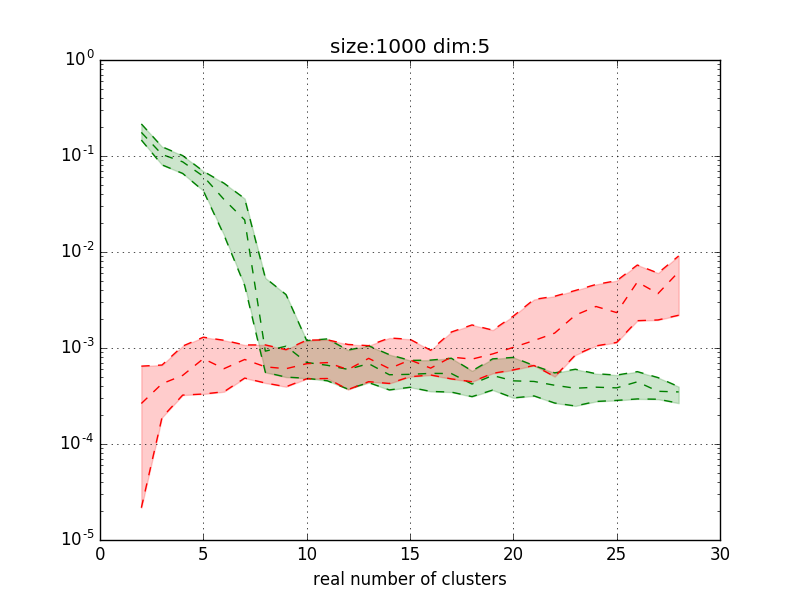
\includegraphics[width=300px]{./TeX_files/SparseWeightsVectorEstimation.png}
  \caption{Vert: Notre algorithme. Rouge: EM+BIC}
\end{figure}
\section{A word on density estimation}

%!TEX root = ../main.tex

\chapter{Partial contributions to clustering}\label{chap:contributions}
In this chapter, we present some work carried out during this thesis which have unfortunately not been able to be the subject of an in-depth study that can be published. The first part deals with the sparsity hypothesis of the precision matrices within a high dimensional Gaussian mixture and adapts the single-component Graphical Lasso from \citep{glasso07} to the mixture setting. In the second part, we assume that the weight vector of the mixture is sparse in order to obtain an estimator of the number of components in the mixture that is generally unknown. 

\section{Graphical Lasso for Gaussian mixtures}\label{chapgraphlasso}
As we saw in the previous sections, the number of free parameters in a full GMM with $K$ components in dimension $p$ are $(K-1)+Kp+Kp(p+1)/2$ which means, for instance, that for $K=5$ and $p=100$ we have $125704$ parameters to estimate. In this high dimensional setting, the EM algorithm experiences severe performance degradation. In particular, the inversion of the covariance matrices are one source of error. One way to circumvent these problems is to use regularization. To this end, we will make a structural assumption on the inverse of the covariance matrices, called precision or concentration matrices, of a component. The work presented in this chapter is inspired by \citep{glasso07}, \citep{banerjee}, \citep{yuanLin_graph} and \citep{meinshausen2006} where it is suggested to penalize the off-diagonal entries of the precision matrix of a Gaussian graphical model. We do an attempt to generalize this work to the Gaussian mixture model.

We consider $\bX=(X^{(1)},\dots,X^{(p)})$, a random vector admitting a $p$-dimensional normal distribution $\mathcal N(\bmu, \bSigma)$ with a non-singular $\bSigma$. One can construct an undirected graph $G=(V,E)$ with $p$ vertices corresponding to each coordinate and, $E=(e_{i,j})_{1\leq i < j \leq p}$, the edges between the vertices describing the conditional independence relation among $X^{(1)},\dots,X^{(p)}$. If in this graph, $e_{i,j}$ is absent in $E$ if and only if $X^{(i)}$ and $X^{(j)}$ are independent conditionally to the other variables $\{X^{(l)}\}$ with $l\neq i,j$ (denoted $X^{(i)} \ci X^{(j)}|X^{(l)}\, l\neq i,j$). Then $G$ is called the Gaussian concentration graph model for the Gaussian random vector $\bX$. 
This representation is particularly interesting in the study of the inverse of the covariance matrix. Let us denote $\bSigma^{-1}=\bOmega=(\omega_{i,j})$ the precision matrix. The entries of this matrix satisfy $\omega_{i,j}=0$ if and only if $X^{(i)} \ci X^{(j)}$ conditionally to all the other variables. We recall in the following lemma this well-known result

\begin{lemma}[Conditional independence in Gaussian concentration graph model]
Consider $\bX=(X^{(1)},\dots,X^{(p)})$, a p-dimensional random vector with a multivariate normal distribution $\mathcal N(\bmu, \bSigma)$, and set $\bSigma^{-1}=\bOmega=(\omega_{i,j})$. Then $X^{(i)} \ci X^{(j)}|\{X^{(l)}: l\notin\{i,j\}\} \iff \omega_{i,j}=0$ with $l\neq i,j$ 
\end{lemma}
\begin{proof}
This result can be found in \citep{edwards2000introduction}. Consider the density of $\bX$
\begin{equation}
  \varphi_{\bmu,\bSigma}(\bx)=\frac{1}{(2\pi)^{p/2}|\bSigma|^{1/2}} \exp\Big(-\frac{1}{2}(\bx-\bmu)^\top\bSigma^{-1}(\bx-\bmu)\Big).
\end{equation}
It can be rewritten as
\begin{equation}
  \varphi_{\bmu,\bSigma}(\bx) = \exp(\alpha + \beta^T\bx-\frac{1}{2}\bx^T\bOmega\bx),
\end{equation}
with $\beta=\bOmega\bmu$ and $\alpha=\frac{1}{2}\log(|\bOmega|)-\frac{1}{2}\bmu^T\bOmega\bmu-\frac{p}{2}\log(2\pi)$. Then, the previous equation can be rewritten as 
\begin{equation}
\label{exp_fam_cond_ind}
  \exp\big(\alpha + \sum_{j=1}^p\beta_jx^{(j)}-\frac{1}{2}\sum_{j=1}^p\sum_{i=1}^p\omega_{i,j}x^{(j)}x^{(i)}\big).
\end{equation}
Now, for three random variables $X,Y,Z$, we have $X \ci Y|Z$ if and only if the joint density can be factorized into two factors $f_{X,Y,Z}(x,y,z)=h(x,z)g(y,z)$, with $h$ anf $g$ two functions. Then, in the light of  \cref{exp_fam_cond_ind}, we have $X^{(i)}\ci X^{(j)}|\{X^{(l)}: l\notin\{i,j\}\} \iff \omega_{i,j}=0$.
\end{proof}
The first result available in the literature on gaussian graphical models focused on the estimation of the graph structure. In particular \citep{dempster1972cov_select} developed a greedy forward or backward search method to estimate the set of non-zero entries in the concentration matrix. The forward method relies on initializing an empty set and selecting iteratively an edge with an MLE fit for $\mathcal{O}(p^2)$ different parameters. The procedure stops according to a suitable selection criterion. The backward method proceeds in the same manner by starting with all edges and operating deletions. It is obvious that such methods are computationally intractable in high dimension. In \citep{meinshausen2006}, the authors studied a neighborhood selection procedure with lasso. The goal is to estimate the neighborhood $ne_{X^{(i)}}$ of a node $X^{(i)}$ which is the smallest subset of $G\setminus\{X^{(i)}\}$ such that $X^{(i)} \ci \big\{X^{(j)}: X^{(j)}\in G\setminus\{ne_{X^{(i)}}\}\big\} | X_{ne_{X^{(i)}}}$. The estimation of the neighborhood is cast as a sparse regression problem and tackled with a lasso penalization. The authors show that this procedure is consistent for sparse high dimensional graphs and computationally efficient. More precisely, let $\theta^{(i)} \in \RR ^p$ be the vector of coefficients of the optimal prediction,
\begin{equation}
  \theta^{(i)} = \argmin_{\theta:\theta_i=0}\EE\Big[\big(X^{(i)}-\sum_{k=1}^p\theta_k X^{(k)}\big)^2\Big],
\end{equation}
then the components of $\theta^{(i)}$ are determined by the precision matrix, $\theta^{(i)}_j=-\omega_{i,j}/\omega_{i,i}$. Therefore, the set of neighbors of $X^{(i)}\in G$ is given by
\begin{equation}
  ne_{X^{(i)}}= \{X^{(j)}, j\in[p]: \omega_{i,j} \neq 0 \}.
\end{equation}
Now, let $\XX$ be the $N\times p$-dimensional matrix such that the column $\XX^{(i)}$ is the vector formed by $N$ of $X^{(i)}$. Given a suitably chosen regularization parameter $\lambda \geq 0$, the Lasso estimate $\hat\theta^{i,\lambda}$ of $\theta^{(i)}$ is defined as
\begin{equation}
  \hat\theta^{i,\lambda} = \argmin_{\theta:\theta_i=0}\Big(\frac{1}{N}\|\XX^{(i)}-\XX\theta \|_2^2 + \lambda\|\theta\|_1 \Big).
\end{equation}
The authors prove under several assumptions that 
\begin{equation}
  P(\hat{ne}_{X^{(i)}}^{\lambda}=ne_{X^{(i)}})\rightarrow 1 \quad \text{when}\quad N\rightarrow \infty,
\end{equation}
and for some $\epsilon > 0$,
\begin{equation}
  P(\hat E^{\lambda}=E)=1-\mathcal{O}(\exp(-cN^{\epsilon}))\quad \text{when}\quad N\rightarrow \infty,
\end{equation}
where $E^{\lambda}$ in a estimate of the edge set. Therefore, this method recovers the conditional independence structure of sparse high-dimensional Gaussian concentration graph at exponential rates. One can estimate the parameters of the model which has been selected by this method using, for instance ordinary least squares. Such a procedure often suffers from the instability of the estimator since small changes in the data change the selected model \citep{yuanLin_graph, breiman1996}. One difficulty of a method that would perform both tasks is to ensure that the estimator of the precision matrix is positive definite. \citep{yuanLin_graph} proposed a penalized-likelihood method that performs model selection and parameter estimation simultaneously as well as ensures the positive definiteness of the precision matrix. Their approach is similar to \citep{meinshausen2006} as they use the $\ell_1$ penalty, they additionally impose a positive definiteness constraint. Furthermore, they replace the residual sum of squares by the negative log-likelihood, 
\begin{equation}
  -\Big\{\frac{N}{2}\log(|\bOmega|) - \frac{1}{2}\sum_{i=1}^N\bX_i^T\bOmega\bX_i\Big\}.
\end{equation}
The resulting constrained minimization problem over the set of positive definite matrices is
\begin{equation}
\label{prec_matrix_gauss_min_pb}
  \text{min}\Big\{-\log(|\bOmega|) + \frac{1}{N}\sum_{i=1}^N\bX_i^T\bOmega\bX_i\Big\} \quad \text{subject to}\quad \sum_{i\neq j} |\omega_{i,j}|\leq t \quad \text{and}\quad \bOmega \succeq 0,
\end{equation}
with $t\geq 0$ a tuning parameter. In these formulae we assume that the mean of the Gaussian distribution is known to be equal to 0. Consider the empirical covariance matrix $\bS=1/N\sum_{i=1}^N\bX_i\bX_i^T$, \cref{prec_matrix_gauss_min_pb} can be rewritten as 
\begin{equation}
  \text{min}\Big\{-\log(|\bOmega|) + \text{tr}(\bS\bOmega)\Big\} \quad \text{subject to}\quad \sum_{i\neq j} |\omega_{i,j}|\leq t.
\end{equation}
Since the whole problem is convex, the Lagrangian is given by
\begin{equation}
\label{yuan_lkhood_pb}
  \mathcal L (\lambda, \bOmega) = -\log(|\bOmega|) + \text{tr}(\bS\bOmega) + \lambda\sum_{i\neq j} |\omega_{i,j}|,
\end{equation}
where $\lambda$ is a tuning parameter. A non-negative garrote-type estimator is provided in \citep{yuanLin_graph} which requires a good initial estimator of $\bOmega$. The authors provided an asymptotic result:
\begin{theorem}[Theorem 1 from \citep{yuanLin_graph}]
If $\sqrt{N}\lambda \rightarrow \lambda_0\geq0$  as $N\rightarrow\infty$, the lasso-type estimator satisfies
\begin{equation*}
  \sqrt{N}(\hat\bOmega-\bOmega)\rightarrow\argmin_{\bU=\bU^T}(\mathcal{V}(\bU)),
\end{equation*}
where the convergence is in distribution and $\mathcal{V}$ is defined by the formula
\begin{equation*}
  \mathcal{V}(\bU)=\textnormal{tr}(\bU \bSigma \bU \bSigma)+\textnormal{tr}(\bU \bW)+\lambda_0\sum_{i\neq j}\big\{ u_{i,j}\textnormal{sign}(\omega_{i,j})I(\omega_{i,j}\neq 0)+|u_{i,j}|I(\omega_{i,j} =0) \big\}
\end{equation*}
in which $\bW$ is a random symmetric $p\times p$ matrix such that $\textnormal{vec}(\bW) \sim \mathcal N (0, \Lambda)$, and  $\Lambda$ is such that
\begin{equation*}
  \textnormal{cov}(w_{i,j},w_{i',j'}) = \textnormal{cov}(X^{(i)}X^{(j)},X^{(i')}X^{(j')}).
\end{equation*}
\end{theorem}
Unfortunately, the computational complexity of interior point methods for maximizing \cref{yuan_lkhood_pb} is $\mathcal O (p^6)$ and at each step, we have to compute and store a Hessian matrix of size $\mathcal O (p^2)$. These prohibitively large complexities led the research on more specialized methods. \citep{banerjee} worked on the same approach, solving a maximum likelihood problem with an $\ell_1$ penalty and focusing on the computational complexity by proposing an iterative block coordinate descent algorithm. The problem to maximize is similar to \cref{yuan_lkhood_pb}
\begin{equation}
\label{max_lkhood_gauss_graph}
  \hat\bOmega = \argmax_{\bOmega \succ 0}\{\log(|\bOmega|)-\textnormal{tr}(\bS\bOmega)-\lambda\|\bOmega \|_1\}.
\end{equation}
Note that the $\ell_1$ norm of a matrix $\bOmega$ can be expressed as
\begin{equation}
  \|\bOmega \|_1 = \max_{\| \bU\|_{\infty}\leq 1}\textnormal{tr}(\bOmega\bU),
\end{equation}
injecting this in \cref{max_lkhood_gauss_graph} gives
\begin{equation}
  \max_{\bOmega \succ 0} \min_{\|\bU\|_{\infty}\leq \lambda} \big\{\log(|\bOmega|)-\textnormal{tr}(\bOmega(\bS+\bU))\big\}.
\end{equation}
After exchanging the min and the max, we solve the problem for $\bOmega$ by setting the gradient to $0$. This gives $(\bOmega^{-1})^T-(\bS+\bU)^T=0$ yielding $\bOmega = (\bS+\bU)^{-1}$. The dual problem is then
\begin{equation}
  \min_{\|\bU \|_{\infty}}\{-\log(|\bS+\bU|) -p\},
\end{equation}
or by setting $\bW = \bS+\bU$,
\begin{equation}
\label{banerjee_min_pb}
  \hat\bSigma = \hat{\bOmega^{-1}}= \argmax \log(|\bW|) \quad \textnormal{s.t}\quad \|\bW-\bS \|_{\infty} \leq \lambda.
\end{equation}
We observe the presence of a log-barrier adding the implicit constraint $(\bS+\bU) \succ 0$. Furthermore, the dual problem estimates the covariance matrix. To solve this maximization problem, the authors proposed a Block Coordinate Descent Algorithm that we describe below (see also \Cref{fig:banerjee_block_algo}). 

\begin{figure}
\begin{center}
\mybox{
\begin{minipage}{1\textwidth}
\begin{algorithmic}[1]%\SetAlgoLined\tt\SetLine
\small
\STATE {\bfseries Input:} Matrix $\bS$, parameter $\lambda$ and threshold $\varepsilon$
\STATE {\bfseries Output:} Estimate of $\bW$
\STATE {{\bf Initialize} $\bW^{(0)} := \bS+\lambda I$}
\REPEAT
\FOR{$j=1,\dots,p$}
\STATE {(a) Let $\bW^{(j-1)}$ denote the current iterate. Solve the quadratic program}
\begin{equation*}
\label{banerjee_algo_min_pb}
  \hat \by := \argmin_{\by}\{\by^T(\bW_{\setminus j \setminus j}^{(j-1)})^{-1}\by:\|\by-\bS_j\|_{\infty}\leq \lambda\}.
\end{equation*}
\STATE {(b) Update the rule: $\bW^{(j)}$ is $\bW^{(j-1)}$ with column/row $\bW_j$ replaced by $\hat\by$.}
\ENDFOR
\STATE{Let $\hat\bW^{(0)}:=\bW^{(p)}$.}
\UNTIL{convergence occurs when
\begin{equation*}
  \textnormal{tr}\big((\hat\bW^{(0)})^{-1}\bS\big) -p +\lambda\big\|(\hat\bW^{(0)})^{-1} \big\|_1\leq \varepsilon.
\end{equation*}
}
\end{algorithmic}
\end{minipage}}
   \caption{Block Coordinate Descent Algorithm}
   \label{fig:banerjee_block_algo}

\end{center}
\end{figure}
It can be proved that the Block Coordinate Descent algorithm converges \citep{banerjee}, achieving an $\varepsilon$-suboptimal solution to \cref{banerjee_min_pb} and each iterate produces a strictly positive definite matrix. For a fixed number of sweeps $K$, the complexity of this algorithm is $\mathcal O (Kp^4)$. They provide also another algorithm using Nesterov's first order method which has a $\mathcal O(p^{4.5}/\epsilon)$ complexity for $\varepsilon > 0$, the desired accuracy. For any symmetric matrix $\bA$, let $\bA_{\setminus k \setminus j}$ be the matrix produced by removing column $k$ and row $j$ from $\bA$. Let $\bA_j$ the $j^{th}$ column of $\bA$ with the element $\bA_{jj}$ removed. It is interesting to note that the dual problem of \Cref{banerjee_algo_min_pb} in \cref{fig:banerjee_block_algo} is 
\begin{equation}
  \min_{\bx} \bx^T\bW_{\setminus j \setminus j}^{(j-1)}\bx - \bS_j^T\bx + \lambda\|\bx\|_1,
\end{equation}
and strong duality holds, it can best casted as
\begin{equation}
\label{banerjee_dual_lasso}
  \min_{\bx} \|\bQ\bx - \bbb\|_2^2 + \lambda\|\bx\|_1,
\end{equation}
with $\bQ = (\bW_{\setminus j \setminus j}^{(j-1)})^{1/2}$ and $\bbb:=\frac{1}{2}\bQ^{-1}\bS_j$. Therefore, we recover the Lasso problem. More precisely, the algorithm can be interpreted as a sequence of iterative Lasso problems. This approach is similar to another paper that we would like to mention \citep{glasso07}. The authors proposed a faster algorithm based on the Block Coordinate Descent algorithm from \citep{banerjee} called Graphical Lasso. They estimate the matrix $\bW=\bOmega^{-1}$ by performing iterative permutations of the columns of this matrix to make the target column the last for a coupled Lasso problem. The matrices $\bW$ and $\bS$ will be presented as following 
\begin{equation}
\bW =  \begin{bmatrix}
    \bW_{11} & \bw_{12} \\
    \bw_{21} & w_{22}
  \end{bmatrix}, 
  \quad
 \bS =  \begin{bmatrix}
    \bS_{11} & \bs_{12} \\
    \bs_{21} & s_{22}
  \end{bmatrix}, 
\end{equation}
and the Graphical Lasso algorithm is described in \Cref{fig:friedman_graph_lasso}. The Lasso problem can be solved via a coordinate descent, the reader can refer to \citep{glasso07} for the procedure. In this problem, the algorithm estimates $\hat\bSigma$ and returns also $\bB = (\bbb^{(1)},\dots,\bbb^{(p)})$, the matrix where each column is the solution of the Lasso problem in \cref{banerjee_dual_lasso} for each column of $\bW$. It is easy then to recover $\bOmega$ since 
\begin{equation}
\bW =  \begin{bmatrix}
    \bW_{11} & \bw_{12} \\
    \bw_{21}^T & w_{22}
  \end{bmatrix}.
  \begin{bmatrix}
    \bOmega_{11} & \bomega_{12} \\
    \bomega_{21}^T & \omega_{22}
  \end{bmatrix}=
   \begin{bmatrix}
    I_{p-1} & \bf{0} \\
    \bf{0}^T & 1
  \end{bmatrix},
\end{equation}
and
\begin{align*}
  \bomega_{12} &= -\bW_{11}^{-1}\bw_{12}\omega_{22}\\
  \omega_{22} &= 1/(w_{22}-\bw_{12}^T \bW_{11}^{-1}\bw_{12}).
\end{align*}
Therefore, for $j=1,\dots,p$, the permuted target components of $\bOmega$ are
\begin{align*}
  \bomega_{12} &= -\bbb^{(j)}\hat\omega_{22}\\
  \omega_{22} &= 1/(w_{22}-\bw_{12}^T \bbb^{(j)}).
\end{align*}
\begin{figure}
\begin{center}
\mybox{
\begin{minipage}{1\textwidth}
\begin{algorithmic}[1]%\SetAlgoLined\tt\SetLine
\small
\STATE {\bfseries Input:} Matrix $\bS$, parameter $\lambda$ and threshold $\varepsilon$
\STATE {\bfseries Output:} Estimate of $\bW$ and $\bB$ a matrix of parameters.
\STATE {{\bf Initialize} $\bW^{(0)} := \bS+\lambda I$ and $\bB=0_{p\times p}$. The diagonal of $\bW$ remained unchanged in what follows.}
\REPEAT
\FOR{$j=1,\dots,p$}
\STATE {(a) Let $\bW^{(j-1)}$ denote the current iterate. Solve the Lasso problem in \cref{banerjee_dual_lasso}
\begin{equation}
  \hat\bx^{(j-1)} = \argmin_{\bx} \frac{1}{2}\|(\bW_{11}^{(j-1)})^{1/2}\bx - \bbb\|_2^2 + \lambda\|\bx\|_1,
 \end{equation}
 with $\bbb:=(\bW_{11}^{(j-1)})^{-1/2}\bs_{12}$.}
\STATE {(b) Update: $\bW^{(j)}$ is $\bW^{(j-1)}$ with $\bw_{12}=\bW_{11}^{(j-1)}\hat\bx^{(j-1)}$. }
\STATE {(c) Save the parameter $\bx^{(j-1)}$ in the $j^{th}$ column of $\bB$.} 
\STATE{(d) Permute the columns and rows of $\bW^{(j-1)}$ such that the $j^{th}$ column is $\bw_{12}$, the next target.}
\ENDFOR
\STATE{Let $\hat\bW^{(0)}:=\bW^{(p)}$.}
\UNTIL{convergence occurs.}
\end{algorithmic}
\end{minipage}}
   \caption{The Graphical Lasso from \citep{glasso07}.}
   \label{fig:friedman_graph_lasso}
\end{center}
\end{figure}
In what follows, we will adapt these methods to a Gaussian mixture model. More precisely, we will assume that each cluster is associated with a sparse Gaussian concentration graph. We will rely on the Graphical Lasso for estimating the precision matrix and will derive an EM algorithm for estimating the model parameters.

\subsection{Graphical Lasso on Gaussian mixtures}
In this part, we present our contribution. We consider a Gaussian mixture model of $K$ components and our task is to estimate the parameters $\btheta=(\theta_1,\dots,\theta_K)$ with $\theta_k=(\pi_k, \bmu_k, \bOmega_k)$, where $\bOmega_k$ is the precision matrix of the $k^{th}$ component of the mixture. We denote $\varphi_{(\bmu_{k},\bOmega_{k})}$ the Gaussian density of mean $\bmu_k$ and precision matrix $\bOmega_k$. The penalized log-likelihood is
\begin{equation}
\label{pen-log-likelihood}
\ell_N^{pen}(\btheta)=\sum_{i=1}^{N}\log p_{\btheta}(\bx_i)-pen(\btheta)= \sum_{i=1}^{N}\log \bigg\{ \sum_{k=1}^K\pi_k\varphi_{(\bmu_{k},\bOmega_{k})}(\bx_i)\bigg\} -pen(\btheta).
\end{equation}
We suppose that each component of the mixture has a sparse Gaussian concentration graph. Therefore, in the spirit of \citep{banerjee} and \citep{glasso07}, we consider an $\ell_1$ regularization $pen(\theta_k)=\sum_{k=1}^K\lambda_k||\bOmega_k||_{1,1}$ with $\lambda_k >0$. The penalization of the log-likelihood concerns only the precision matrices $\bOmega_k$. Regarding the other parameters $(\pi_k, \bmu_k)$, our algorithm is the same as EM and we can use the same iteration technique as in \Cref{lemma1} to maximize the following cost function
\begin{equation}
\label{cost_fun_pen}
F^{pen}(\btheta,\bTau)  = \sum_{k=1}^K \bigg(\sum_{i=1}^{N} \Big\{\tau_{i,k}\log\varphi_{\bmu_{k},\bOmega_{k}}(\bx_i)+\tau_{i,k}
    \log(\pi_k/\tau_{i,k})\Big\}-\lambda_k||\bOmega_k||_{1,1}\bigg).
\end{equation}
The maximization of this function over $\btheta$ and $\bTau$ leads to the two following optimization problems:
\begin{align}
\label{optim-problems}
\hat\btheta(\bTau)&\in \arg\max_{\btheta} F^{pen}(\btheta,\bTau),\qquad \hat\bTau(\btheta)\in \arg\max_{\bTau} F^{pen}(\btheta,\bTau).
\end{align}
For a given $\hat\bTau$, estimates of $(\pi_1,\dots,\pi_K)$ and $(\bmu_1,\dots,\bmu_K)$ obtained by the first optimization problem in \cref{optim-problems} are the same as in the EM algorithm:
\begin{align}
\label{em-sols}
\hat\pi_k     &= \frac1N\sum_{i=1}^N \hat\tau_{i,k},\quad\text{and}\quad\hat\bmu_k = \frac1{N\hat\pi_k}\sum_{i=1}^N \hat\tau_{i,k}\bx_i \qquad \forall k\in[K],
\end{align}
and for a given $\hat\btheta$, the estimate of $\bTau$ obtained by the second optimization problem is
\begin{equation}
\label{em-sols-tau}
\hat\tau_{i,k} = \text{P}_{\btheta}(Z=k|\bX=\bx_i)=\frac{\hat\pi_k\varphi_{\hat\bmu_k,\hat\bOmega_k}(\bx_i)}{\sum_{k'\in[K]}\hat\pi_{k'}\varphi_{\hat\bmu_{k'},\hat\bOmega_{k'}}(\bx_i)},\qquad\forall k\in[K],\ \forall i\in[N].
\end{equation}
However, due to the penalty $\lambda_k||\bOmega_k||_{1,1}$, the estimation of $\bOmega_k$ is not straightforward. To overcome this problem, let us introduce the weighted empirical covariance matrix
\begin{equation}
\bSigma_{N,k} = \frac{1}{N}\frac{\sum_{i=1}^N\tau_{i,k}(\bx_i-\hat\bmu_k)(\bx_i-\hat\bmu_k)^\top}{\sum_{i=1}^N\tau_{i,k}}.
\end{equation}
The penalized log-likelihood in equation \eqref{cost_fun_pen} can therefore be expanded as following
\begin{align*}
\label{cost_fun_pen_2}
F^{pen}(\btheta,\bTau)  =& \sum_{k=1}^K \bigg( \sum_{i=1}^{N}\Big\{ \tau_{i,k} \Big(
-\frac{p}{2}\log(2\pi)+\frac{1}{2}\log|\bOmega_k|
-\frac{1}{2}(\bx_i-\bmu_k)^T\bOmega_k(\bx_i-\bmu_k) \Big)\\
&+\tau_{i,k} \log(\pi_k/\tau_{i,k})\Big\} -\lambda_k||\bOmega_k||_{1,1}\bigg)\\
=& -\frac{Np}{2}\log(2\pi)+\sum_{k=1}^K \bigg(\frac{N\pi_k}{2}\log|\bOmega_k|\\
&+\sum_{i=1}^{N}\Big\{ -\frac{\tau_{i,k}}{2}(\bx_i-\bmu_k)^T\bOmega_k(\bx_i-\bmu_k)+\tau_{i,k} \log(\pi_k/\tau_{i,k})\Big\} -\lambda_k||\bOmega_k||_{1,1}\bigg). 
\end{align*}
Hence, the opposite minimization problem regarding each $\bOmega_k$ is
\begin{equation}
\bOmega_k \in \argmin_{ \bOmega\succeq 0}\Big\{-\frac{N\pi_k}{2}\log|\bOmega|+\frac{1}{2}\sum_{i=1}^{N}\tau_{i,k}(\bx_i-\bmu_k)^T\bOmega(\bx_i-\bmu_k)+\lambda_k||\bOmega||_{1,1}\Big\}.
\end{equation}
And using the well-known commutativity property of the trace operator and dividing by $N\pi_k$ gives
\begin{equation}
\bOmega_k \in \argmin_{ \bOmega\succeq 0} \Big\{ -\frac{1}{2}\log|\bOmega| +\frac{1}{2} tr(\bSigma_{N,k}\bOmega)+\frac{\lambda_k}{N\pi_k}||\bOmega||_{1,1}\Big\}.
\end{equation}
In the light of this equation, one can notice that we solve a graphical lasso problem within each cluster. This minimization problem is convex and can be solved with a block coordinate ascent algorithm as described in \citep{mazum_lasso}. This results in an EM-like alternating minimization procedure summarized in \Cref{algo:graph_lasso_EM}.
\begin{figure}
\begin{center}
\mybox{
\begin{minipage}{0.85\textwidth}
\begin{algorithmic}%\SetAlgoLined\tt\SetLine
\small
\STATE {\bfseries Input:} Observations $\bx_1,\ldots,\bx_N\in\RR^p$ and the number of clusters $K$.
\STATE {\bfseries Output:} Parameter estimate $\hat\btheta = \{\hat\bmu_k,\hat\bOmega_k,\hat\pi_k\}_{k\in[K]}$
\STATE {\tt 1:} Initialize $t=0$, $\btheta=\btheta^0$.
\FOR{$t=1,\dots$, until convergence occurs,}
\STATE {\tt 2:} \qquad Update the parameter $\bTau$:
\begin{align*}
\tau_{i,k}^{t}  &= \frac{\pi_k^{t}\varphi_{\bmu_k^{t},\bOmega_k^{t}}(\bx_i)}{\sum_{k'\in[K]}\pi^{t}_{k'}\varphi_{\bmu^{t}_{k'},\bOmega^{t}_{k'}}(\bx_i)}.
\end{align*}
\STATE {\tt 3:} \qquad Update the parameter $\btheta$ for each component:
\begin{align*}
\pi_k^{t+1}     &= \frac1N\sum_{i=1}^N \tau_{i,k}^t,\qquad \\
\bmu_k^{t+1}    &= \frac1{N\pi_k^{t+1}}\sum_{i=1}^N \tau_{i,k}^t\bx_i\\
\bSigma_{n,k}         &= \frac{1}{N^2\pi_k^{t+1}}\sum_{i=1}^N\tau_{i,k}^{t+1}(\bx_i-\hat\bmu_k^{t+1})(\bx_i-\hat\bmu_k^{t+1})^\top\\
\bOmega_k^{t+1} & \in \argmin_{ \bOmega\succeq 0} \Big\{ -\frac{1}{2}\log| \bOmega |+\frac{1}{2} tr(\bSigma_{N,k}\bOmega)+\frac{\lambda_k}{n\pi_k^{t+1}}||\bOmega||_{1,1}\Big\}
\end{align*}
\ENDFOR
\end{algorithmic}
\end{minipage}}
   \caption{Graphical lasso algorithm for Gaussian mixtures.}
   \label{algo:graph_lasso_EM}
\end{center}
\end{figure}
\todos{regenerer les graphes et une conclusion, mentionner que ca a ete deja fait dans (cite)}

\begin{figure}
        \captionsetup[subfigure]{aboveskip=-1pt}
        \centering
        \begin{subfigure}[b]{\textwidth}
                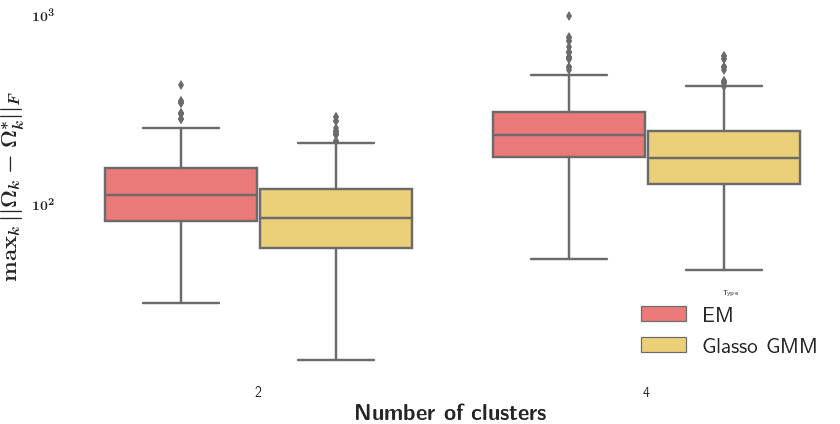
\includegraphics[width=0.8\textwidth]{TeX_files/graph_lasso_2_100.png} 
                \caption{p=2, N=100}
                \label{fig:glasso_dim2_N100}
        \end{subfigure}       
        \begin{subfigure}[b]{\textwidth}
                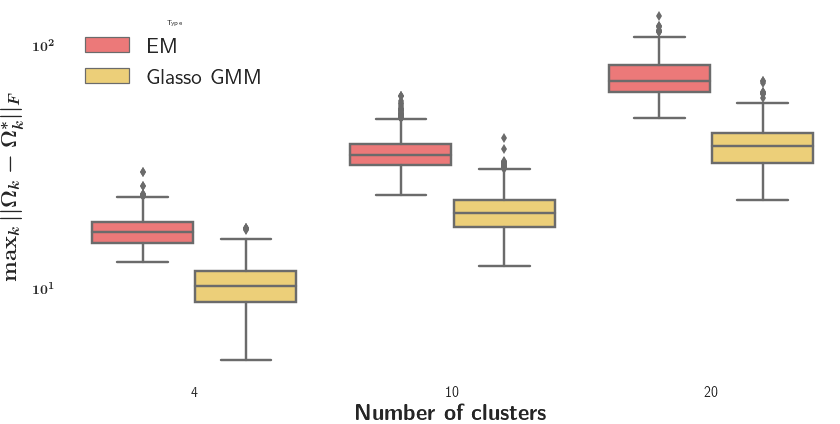
\includegraphics[width=0.8\textwidth]{TeX_files/graph_lasso_5_1000.png}
                \caption{p=5, N=1000}
                \label{fig:glasso_dim5_N1000}
        \end{subfigure}
        \caption{Estimation with glasso on GMM}\label{fig:glasso_res_simu} 
\end{figure}

\begin{figure}

        \begin{subfigure}[b]{\textwidth}
                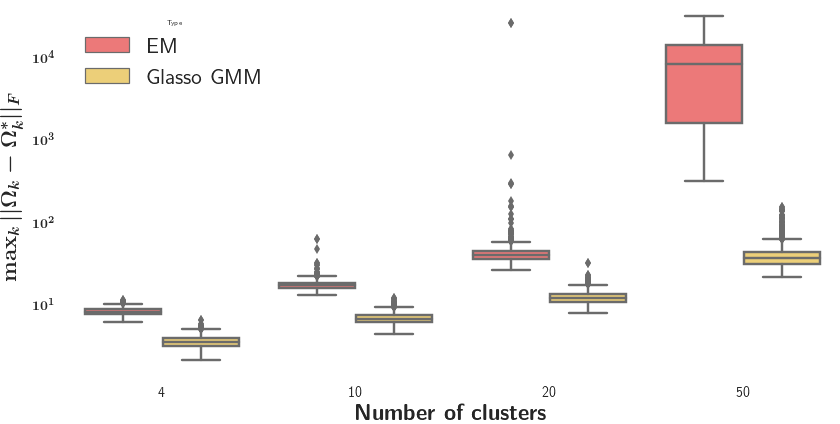
\includegraphics[width=0.8\textwidth]{TeX_files/graph_lasso_10_1000.png} 
                \caption{p=10, N=1000}
                \label{fig:glasso_dim10_N1000}
        \end{subfigure}       
        \begin{subfigure}[b]{\textwidth}
                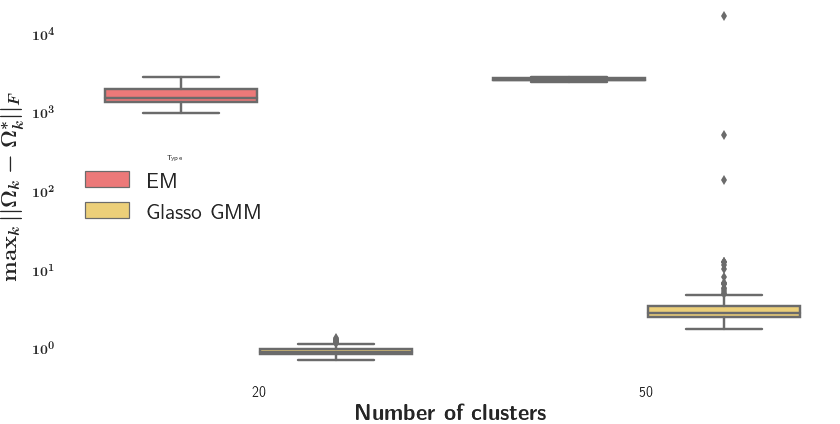
\includegraphics[width=0.8\textwidth]{TeX_files/graph_lasso_50_1000.png}
                \caption{p=50, N=1000}
                \label{fig:glasso_dim50_N1000}
        \end{subfigure}
        \caption{Estimation with glasso on GMM}\label{fig:glasso_res_simu2} 
\end{figure}

\begin{figure}

        \begin{subfigure}[b]{\textwidth}
                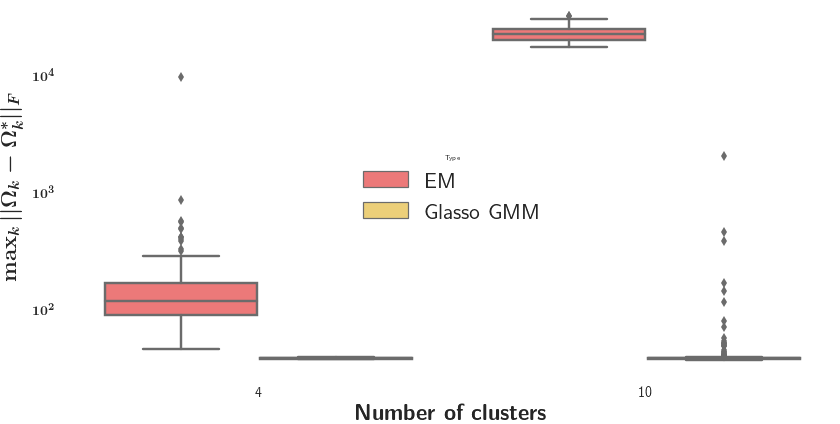
\includegraphics[width=0.8\textwidth]{TeX_files/graph_lasso_diag_upper10_100.png} 
                \caption{p=10, N=100, upper diag}
                \label{fig:glasso_dim10_N100_ud}
        \end{subfigure}       
        \begin{subfigure}[b]{\textwidth}
                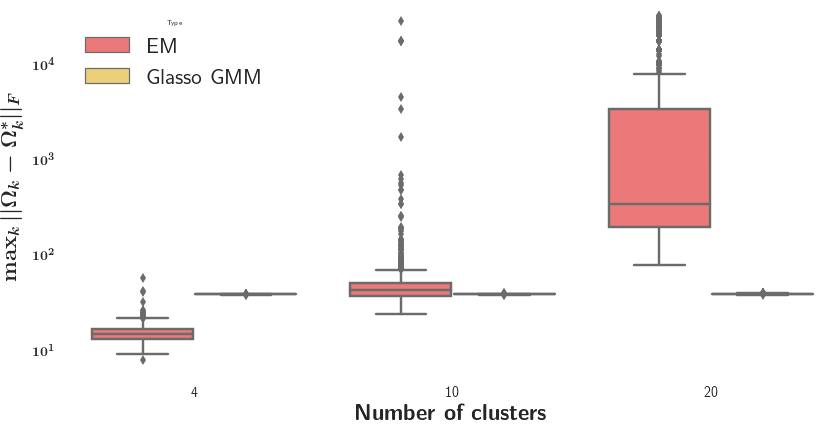
\includegraphics[width=0.8\textwidth]{TeX_files/graph_lasso_diag_upper10_500.png}
                \caption{p=10, N=500, upper diag}
                \label{fig:glasso_dim10_N500_ud}
        \end{subfigure}
        \caption{Estimation with glasso on GMM}\label{fig:glasso_res_simu2} 
\end{figure}
\begin{figure}

        \begin{subfigure}[b]{\textwidth}
                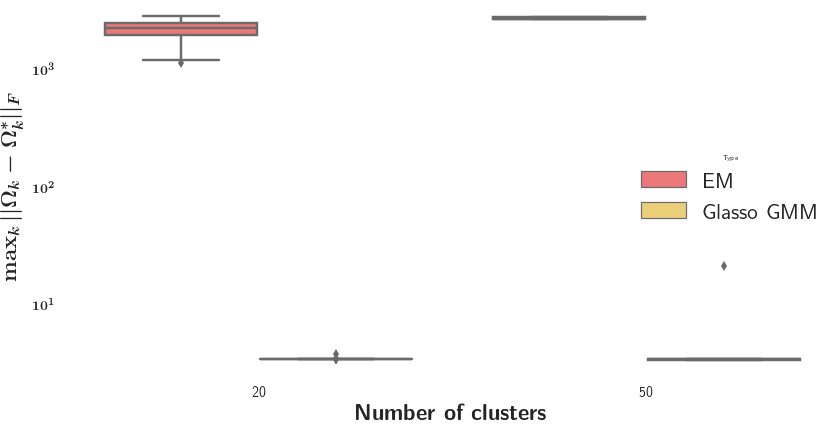
\includegraphics[width=0.8\textwidth]{TeX_files/graph_lasso_diag_upper50_1000.png} 
                \caption{p=50, N=1000, upper diag}
                \label{fig:glasso_dim50_N1000_ud}
        \end{subfigure}       
        \caption{Estimation with glasso on GMM}\label{fig:glasso_res_simu2} 
\end{figure}

\section{Estimating the number of clusters}
\label{estim_nb_clusters_sect}

In this section, we will focus on the problem of estimating the number of clusters, $K$, in a Gaussian mixture model. Most of popular clustering methods such as K-Means, Expectation-Maximization with Gaussian mixture model or spectral clustering need this parameter in input. Different methods are being used to perform a selection of the best model according to a criterion, unfortunately with a computational cost. As we saw in \Cref{sec:finding_clusters_nb}, we generally have to perform multiple clusterings with the parameter $K$ ranging from say 2 to $K_{max}$, where $K_{max}$ is a the maximum number of clusters we assume are present in the dataset, and select the best model according to a criterion. In this work, we seek to adapt the EM algorithm with an `adaptive' sparse estimation of the weight vector of the Gaussian components.

\subsection{First method: regularizing the posteriors}\label{sec:tau_pen_estim}
Our first approach was to penalize the matrix of posteriors $\bTau$ defined in \Cref{sec:EM_algo}. Given $N$ $p$-dimensional observations $\bx_1,\dots,\bx_N$, let us consider the EM algorithm with a number of clusters $K_{max}$ that we know is greater than the true number of clusters. The idea of this method is to add a regularization term on the estimation of the $N\times K_{max}$ matrix $\bTau$, the component $\tau_{i,j}$ of which, we recall, is defined as 
\begin{equation}
  \tau_{i,j} = p_{\btheta}(Z=j | \bX=\bx_i) = \frac{\pi_j\varphi_{\bmu_j,\bSigma_j}(\bx_i)}{\sum_{k=1}^{K_{max}}\pi_k\varphi_{\bmu_k,\bSigma_k}(\bx_i)}.
\end{equation}
The estimate number of clusters $\hat K$ will be the number of non-empty columns of $\bTau$. Let us consider the probability simplex in $\RR^{K_{max}}$, $\bPi\coloneqq \{\btau \in \RR^{K_{max}} : \sum_{k=1}^{K_{max}}\tau_k=1, \tau_k\geq 0 \quad \forall k \in [K_{max}] \}$ and the indicator function $\chi_{\bPi}(.)$ defined as
\begin{equation*}
    \chi_{\bPi}(\btau) =
    \begin{cases}
      0 & \text{if } \btau \in \bPi,\\
        +\infty & \text{elsewhere}.
    \end{cases}
\end{equation*}
We note $\bTau_{.,k}$ the $k^{th}$ column and $\bTau_{i,.}$ the $i^{th}$ line of $\bTau$. Using the cost function in \Cref{cost_gmm_em} and adding an $L_2$ penalization term of the columns of $\bTau$ with a parameter $\lambda > 0$, we have the following cost function for our problem:
\begin{align*}
F^{pen}(\btheta,\bTau)  =& -\sum_{k=1}^K \bigg(\sum_{i=1}^{n} \Big\{\tau_{i,k}\log\varphi_{\bmu_{k},\bOmega_{k}}(\bx_i)+\tau_{i,k}\log(\frac{\pi_k}{\tau_{i,k}})\Big\}\bigg)\\
&+ \lambda\sum_{k=1}^K \|\bTau_{.,k}\|_{2} + \sum_{i=1}^{n} \chi_{\bPi}(\bTau_{i,.}),
\end{align*}
 and the expectation step in EM consists on the following optimization problem:
\begin{equation}
\hat\bTau(\btheta)\in \argmin_{\bTau} F^{pen}(\btheta,\bTau).
\end{equation}
A nice property of this problem is that it is convex. Unfortunately, the regularization term prevents to derive an explicit solution. Furthermore, we cannot separate the objective function since we optimize along columns and lines of $\bTau$. The objective function $F^{pen}(\btheta,\bTau)$ rewritten $F^{pen}_{\btheta}(\bTau)$ can be split into two terms:
\begin{equation}
F^{pen}_{\btheta}(\bTau)={\large f}({\footnotesize\bTau})+ {\large g}({\footnotesize\bTau})
\end{equation}

with
\begin{align*}
f(\bTau) =& -\sum_{k=1}^K \bigg(\sum_{i=1}^{n} \Big\{\tau_{i,k}\log\varphi_{\bmu_{k},\bOmega_{k}}(\bx_i)+\tau_{i,k} \log(\pi_k/\tau_{i,k})\Big\} + \sum_{k=1}^K \|\bTau_{.,k}\|_{2},\\
g(\bTau) =& \sum_{i=1}^{n} \chi_A(\bTau_{i,.}).
\end{align*}
Note that $f$ is convex and differentiable on its domain, $g$ is also convex but not differentiable. We will tackle this problem by using a proximal method (see \citep{Parikh:2014:PA:2693612.2693613} for more details), the $(k+1)^{th}$ step is given by
\begin{align*}
  \bTau^{k+1} &= {\bf{prox}}_{g}(\bTau^k - \eta \nabla f(\bTau^k))\\
      &= \textnormal{P}_{\bPi}(\bTau^k - \eta \nabla f(\bTau^k))\\
      &=\argmin_{ \bTau : \forall i, \bTau_{i,.} \in \bPi}\big( \| \bTau - (\bTau^k - \eta \nabla f(\bTau^k) ) \|^2_2 \big),
\end{align*}
where $\textnormal{P}_{\bPi}$ is the projection function on $\bPi$. The gradient of f on $\bTau$ is given by
\begin{equation}
\bigg[\nabla_{\bTau}f(\bTau)\bigg]_{i,j} = 
1+\frac{\tau_{i,j}}{||\bTau_{.,j}||_2}-\log(\varphi_{\bmu_j,\bOmega_j}(\bx_i))-\log(\frac{\pi_j}{\tau_{i,j}})
\end{equation}
We use the algorithm FISTA \citep{Beck:2009:FIS:1658360.1658364} for this iteration procedure, we provide more details on this method in \Cref{mle_kl_estim_impl}. The implementation of this method is given in \Cref{algo:Pen_tau_EM_expect}, the whole EM-like method for the estimation of the parameters of the GMM is given in \Cref{algo:Pen_tau_EM}. 
\begin{figure}
\begin{center}
\mybox{
\begin{minipage}{0.85\linewidth}
\begin{algorithmic}%\SetAlgoLined\tt\SetLine
\small
\STATE {\bfseries Input:} Parameters $\btheta=(\bmu,\bSigma,\bpi)$
\STATE {\bfseries Output:} Estimate $\hat\bTau$
\STATE {\tt 1: Initialize $t_0=1$ and $\bxi^0$ with}
\begin{align*}
\xi_{i,k}^{0}  &= \frac{\pi_k^{0}\varphi_{\bmu_k^{0},\bOmega_k^{0}}(\bx_i)}{\sum_{k'\in[K]}\pi^{0}_{k'}\varphi_{\bmu^{0}_{k'},\bOmega^{0}_{k'}}(\bx_i)}
\end{align*}
\FOR{$k\geq 1,$ until convergence occurs, }
\STATE {(a) $\bTau^k =\argmin_{ \bTau : \forall i, \bTau_{i,.} \in \bPi}\big( \| \bTau - (\bxi^k - \lambda \nabla f(\bxi^k) ) \|^2_2 \big)$,}
\STATE {(b) $t_{k+1}= \frac{1+\sqrt{1+4t_k^2}}{2}$,}
\STATE {(c) $\bxi_{k+1} = \bTau^k + \bigg( \frac{t_k-1}{t_{k+1}}\bigg) \big( \bTau^k - \bTau^{k-1} \big)$.}
\ENDFOR
\end{algorithmic}
\end{minipage}}
   \caption{Expectation step, estimation of $\bTau$ with FISTA.}
   \label{algo:Pen_tau_EM_expect}
\end{center}
\end{figure}

\begin{figure}
\begin{center}
\mybox{
\begin{minipage}{0.85\linewidth}
\begin{algorithmic}%[1]\tt
%\SetLine%\SetAlgoLined
\small
\STATE {\bfseries Input:} Observations $\bx_1,\ldots,\bx_N\in\RR^p$ and the number of clusters $K$
\STATE {\bfseries Output:} Parameter estimate $\hat\btheta = \{\hat\bmu_k,\hat\bSigma_k,\pi_k\}_{k\in[K]}$
\STATE {\tt 1:} Initialize $t=0$, $\btheta=\btheta^0$.
\STATE {\tt 2:} {\bf Repeat}
\STATE \qquad {\tt 3:} Update the parameter $\bTau$ by using the procedure given in \Cref{algo:Pen_tau_EM_expect}.
\STATE \qquad{\tt 4:} Update the parameter $\btheta$:
\begin{align*}
\pi_k^{t+1}     &= \frac1N\sum_{i=1}^N \tau_{i,k}^t,\qquad
\bmu_k^{t+1}    = \frac1{N\pi_k^{t+1}}\sum_{i=1}^N \tau_{i,k}^t\bx_i,\\
\bSigma_k^{t+1} &= \frac1{N\pi_k^{t+1}}\sum_{i=1}^N \tau_{i,k}^t(\bx_i-\bmu_k^{t+1})(\bx_i-\bmu_k^{t+1})^\top.
\end{align*}
\STATE \qquad {\tt 5:} increment $t$: $t=t+1$.
\STATE {\tt 6:} {\bf Until} stopping rule.
\STATE {\tt 7:} {\bf Return} $\btheta^{t}$.
\end{algorithmic}
\end{minipage}}
   \caption{EM algorithm with penalization on the columns of $\bTau$.}
   \label{algo:Pen_tau_EM}
\end{center}
\end{figure}
A major drawback of this method is the computational cost in \Cref{algo:Pen_tau_EM_expect} of minimizing over the set of $N\times K_{max}$ matrices and we didn't manage to get interesting results for this algorithm.\todos{tentative de sortir des graphs en cours}

\subsection{Second method: penalizing the weights vector}
\label{sparse_weight_vect_estim}
The second approach that we took in order to have an estimate of the number of clusters, i.e. select an appropriate model, was to penalize the weights vector of the Gaussian mixture. The idea is similar to the previous method with an EM-like algorithm maximizing a penalized log-likelihood. Let $\lambda > 0$ be a parameter of penalization and consider the following negative penalized log-likelihood:
\begin{equation}
  \ell_N(\btheta)=
-\frac{1}{N}\sum_{i=1}^{N}\log\bigg\{{\sum_{j=1}^K\pi_k\varphi_{(\bmu_{j},\bSigma_{j})}(\bx_i)}\bigg\}+\lambda\sum_{j=1}^{K}\pi_j^{1/\gamma}\quad \gamma\geq1,
\end{equation}
such that:
\begin{equation}
  \forall j\in[K], \pi_j \geq 0 \quad \text{and} \quad \sum_{j}^{K}\pi_j=1.
\end{equation}
One may wonder why choosing such penalization ? The aim is to promote the merging of similar clusters. For instance, let us consider 2 similar clusters (similar means and covariance matrices) with a weight vector $\bpi=(1/2, 1/2)$ and the merged cluster with weight $\bpi'=(1)$. It is obvious that the log-likelihoods are the same. By choosing the $L_1$ norm, the weight vector $\pi_1+\pi_2$ leads to a penalty equal to 1 which is the same that taking the merged cluster with a weight and penalty equal to 1. However, by taking the penalty $\pi_1^{\nicefrac{1}{2}}+\pi_2^{\nicefrac{1}{2}}$ we have a penalty for the two clusters equal to $2/\sqrt{2}\sim 1.4$. Hence, the method will promote the solution with one cluster. Let us consider the $K$-dimensional probability simplex $\BB^+_K=\{\bpi\in \RR^K: \forall j\in[K], \pi_j \geq 0,\,  \sum_{j}\pi_j=1\}$. Our method is similar to EM in the expectation step and in the maximization step for estimating $\bmu_k$ and $\bSigma_k$, it differs on the estimation of the weights vector $\bpi$ by solving the following minimization problem:
\begin{equation}
  \hat\bpi= \argmin_{\bpi\in\BB^+_K}\bigg\{
-\frac{1}{N}\sum_{i=1}^{N}\log\Big({\sum_{j=1}^K\pi_k\varphi_{(\bmu_{j},\bSigma_{j})}(\bx_i)}\Big)+\lambda\sum_{j=1}^{K}\pi_j^{1/\gamma}\bigg\} \quad \gamma\geq1.
\end{equation}
Unfortunately, $\sum_{j}\pi_j^{1/\gamma}$ is not convex, we solve this problem by making a change of variable, let us note $\alpha_j = \pi_j^{1/\gamma}$ and consider the problem:
\begin{equation}
\hat\balpha\in\argmin_{\balpha\in \RR^{K}}\bigg\{
-\frac{1}{N}\sum_{i=1}^{N}\log\Big\{{\sum_{j=1}^K\alpha^\gamma_j\varphi_{(\bmu_{j},\bSigma_{j})}(\bx_i)}\Big\}+\lambda\sum_{j=1}^{K}\alpha_j \color{black} \bigg\}\quad \gamma\geq1,  
\end{equation}
with  $\forall j \in[K]\, \alpha_j^\gamma \geq0\ \text{and}\ \sum_{j}\alpha^\gamma_{K}=1$. This is a convex problem and we can recover an estimate $\hat\bpi=(\hat\alpha_1^{\gamma},\dots,\hat\alpha_K^{\gamma})$. The first term of this objective function is convex and differentiable with respect to $\balpha$, we note it $f_\btheta(\balpha)$. However, the second term, is convex but not differentiable w.r.t. $\balpha$. As we saw in the previous section, we can use an iterative proximal method to solve this problem. Let us consider $\gamma\geq 0$ and define $A_{\gamma}=\{\balpha\in\RR^K: \forall j \in[K]\, \alpha_j^\gamma \geq0\ \text{and}\ \sum_{j}\alpha^\gamma_{K}=1 \}$. If we consider {\large$\chi_{A_{\gamma}}$}, the indicator function of $A_{\gamma}$ ($0$ in $A_{\gamma}$, $\infty$ elsewhere), the minimization problem can be rewritten as
\begin{equation}
  \hat\balpha\in\argmin_{\balpha\in\RR^{K}}\{ f_\btheta(\balpha) + \chi_{A_{\gamma}}  \},
\end{equation}
and the $(t+1)^{th}$ step of the iterative proximal procedure is:
\begin{align}
\hat\balpha^{t+1}
&={\text{prox}}_{\chi_{A_{\gamma}}}( \balpha^t - h \nabla f_{\btheta}(\balpha^t)  )\\
&=\argmin_{x\in\RR^{K}}\Big\{ \chi_{A_{\gamma}}(x) + \frac{1}{2}\|x-(\balpha^t - h \nabla f_{\btheta}(\balpha^t)) \|^2 \Big\}\\
&=\textnormal{P}_{A_{\gamma}}(\balpha^t - h \nabla f_{\btheta}(\balpha^t) ),
\end{align}
with $h>0$ a gradient step, and for $j\in[K]$, the gradient of $f_{\btheta}$ w.r.t $\balpha$ is
\begin{equation}
  \Big[\nabla f_{\btheta}(\balpha)\Big]_{j} = -\frac{1}{N}\sum_{i=1}^N\frac{\gamma\alpha_j^{\gamma-1}\varphi_{\bmu_j,\bSigma_j}(\bx_i)}{\sum_{k=1}^K\alpha_k^{\gamma}\varphi_{\bmu_k,\bSigma_k}(\bx_i)}+\lambda.
\end{equation}
The FISTA procedure for estimating $\hat\balpha$ is given in \Cref{algo:alpha_fista_proc}. Note that we relaxed the constraints by estimating the $K-1$ components of $\balpha$ since $\alpha_K=1-\sum_{k=1}^{K-1}\alpha_k$. The set $A_{\gamma}$ is redefined accordingly: $A=\{\balpha\in\RR^{K}: \sum_{k=1}^{K-1}\alpha_k\leq1,\, \alpha_K=1-\sum_{k=1}^{K-1}\alpha_k\}$. The final EM-like iteration procedure for estimating the parameters of a Gaussian mixture with penalization of the weights vector is given in \Cref{algo:EM_alpha_pen}.
\begin{figure}[H]
\begin{center}
\mybox{
\begin{minipage}{0.85\linewidth}
\begin{algorithmic}%\SetAlgoLined\tt\SetLine
\small
\STATE {\bfseries Input:} Parameter $\btheta=\{(\bmu_k,\bSigma_k,\bpi)_{k\in[K]}\}$.
\STATE {\bfseries Output:} Parameter estimate $\hat\balpha = \big(\balpha_1,...,\balpha_{K-1},1-\sum_{j=1}^{K-1}\balpha_j).$
\STATE {\tt 1:} Initialize $t_0=1$ and $\xi^0=(\bpi_1^{1/\gamma},...,\bpi_{K-1}^{1/\gamma})$.
\FOR{$k\geq1$, until convergence occurs, }
\STATE {(a) $\balpha^k =\textnormal{P}_A(\xi^k - h \nabla f_{\btheta}(\xi^k))$,}
\STATE {(b) $t_{k+1} = \frac{1+\sqrt{1+4t_{k+1}^2}}{2}$}
\STATE {(c) $\bxi^{k+1} = \balpha^t + \bigg( \frac{t_k-1}{t_{k+1}}\bigg) \big( \balpha^k - \balpha^{k-1} \big)$}
\ENDFOR
\end{algorithmic}
\end{minipage}}
   \caption{Estimation of $\balpha$ via the FISTA method. }
   \label{algo:alpha_fista_proc}
\end{center}
\end{figure}
\begin{figure}[H]
\begin{center}
\mybox{
\begin{minipage}{0.85\linewidth}
\begin{algorithmic}%\SetAlgoLined\tt\SetLine
\small
\STATE {\bfseries Input:} Observations $\bx_1,\ldots,\bx_N\in\RR^p$ and a number of clusters $K_{max}$.
\STATE {\bfseries Output:} parameter estimate $\hat\btheta = \{\hat\bmu_k,\hat\bSigma_k,\hat\pi_k\}_{k\in[K]}$
\STATE {\tt 1:} Initialize $t=0$, $\btheta=\btheta^0$.
\FOR{$t=1,\dots$, until convergence occurs,}
\STATE {\tt 2:} Update the parameter $\bTau$:
\begin{equation*}
\tau_{i,k}^{t}  = \frac{\pi_k^{t}\varphi_{\bmu_k^{t},\bSigma_k^{t}}(\bx_i)}{\sum_{k'\in[K]}\pi^{t}_{k'}\varphi_{\bmu^{t}_{k'},\bSigma^{t}_{k'}}(\bx_i)}.
\end{equation*}
\STATE {\tt 3:} Update the parameter $\hat\balpha^{t+1}$ with algorithm in \Cref{algo:alpha_fista_proc} and compute $\hat\bpi^{t+1}=((\alpha_1^{t+1})^{\gamma}),\dots,(\alpha_K^{t+1})^{\gamma})$.
\STATE {\tt 4:} Update parameters $(\bmu_k,\bSigma_k)$ for $k\in[K_{max}]$:
\begin{align*}
\bmu_k^{t+1}    &= \frac1{n\pi_k^{t+1}}\sum_{i=1}^n \tau_{i,k}^t\bx_i,\\
\bSigma_k^{t+1} &= \frac1{n\pi_k^{t+1}}\sum_{i=1}^n \tau_{i,k}^t(\bx_i-\bmu_k^{t+1})(\bx_i-\bmu_k^{t+1})^\top.
\end{align*}
\ENDFOR
\end{algorithmic}
\end{minipage}}
   \caption{Algorithm for estimating sparse weights vector on GMM.}
   \label{algo:EM_alpha_pen}
\end{center}
\end{figure}
We generated different mixtures with $K$ varying from 2 to 30 components in dimension 5 and draw $N=1000$ observations. We compared our algorithm with EM and the BIC selection method with $K_{max}=2*K$. The resulting weight vectors are compared with the true weight $\bpi^*$ in $L_1$ norm. The plot of our simulations are given in \Cref{fig:results_alpha_pen}. In the horizontal axis, the number of real clusters in the mixture and in the vertical axis the error  $\|\hat\bpi-\bpi^*\|_1$. We ran 50 simulations, the first and third quartiles are shown as long as the median on each regions. As we can see, our algorithm shows promising results. With a small number of clusters, the estimation error $\|\hat\bpi-\bpi^*\|_1$ of our algorithm (green) is greater than with EM-BIC (red). However, when the number of clusters $K$ increases the estimation error of our algorithm decreases whereas the estimation error of EM-BIC increases. Such phenomenon of decreasing error while the complexity increase is not logical, we are confident that a more careful choice of the penalization parameter $\lambda$ would improve the error in low regime showing a slightly increasing curve, still better than EM-BIC.
\begin{figure}
\center
  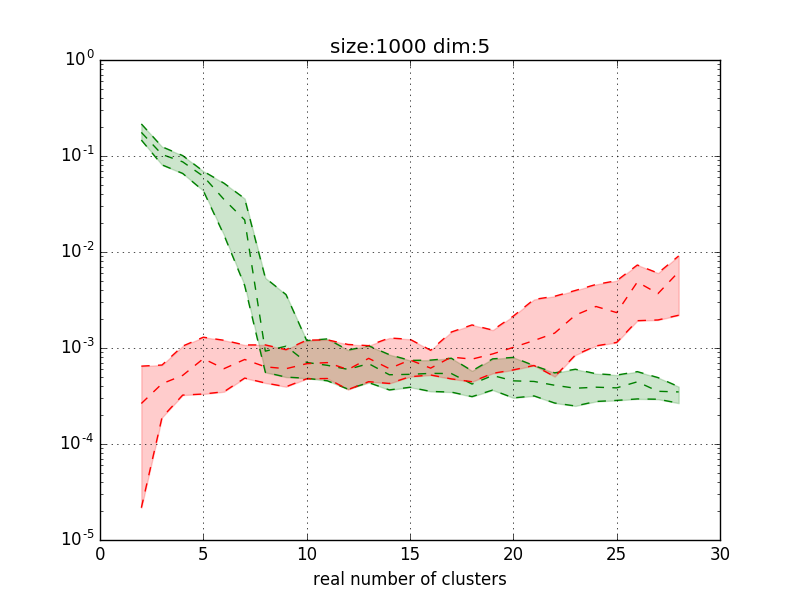
\includegraphics[scale=0.5]{./TeX_files/SparseWeightsVectorEstimation.png}
  \caption{Estimation error $\|\hat\bpi-\bpi^*\|_1$, for our algorithm (green) and EM-BIC (red). Vertical axis: error $\|\hat\bpi-\bpi^*\|_1$ in log scale, horizontal axis: real number of clusters. First and third quartiles are shown as long as the median.}
  \label{fig:results_alpha_pen}
\end{figure}
\todos{mentionner que cette approche est similaire avec les chapitres suivant sur le MLE}

%include{TeX_files/02-cluster_number_estim}
%%!TEX root = ../main.tex

\chapter{Algorithm 2}

We consider the diagonal matrix $D_{\lambda}=diag(\lambda_1,\dots,\lambda_K)$.
\begin{figure}
\begin{center}
\mybox{
\begin{minipage}{0.85\linewidth}
\begin{algorithmic}%[1]\tt
%\SetLine%\SetAlgoLined
\small
\STATE {\bfseries Input:} data vectors $\bx_1,\ldots,\bx_n\in\RR^p$, the number of clusters $K$ and $D_{\lambda}$
\STATE {\bfseries Output:} parameter estimate $\hat\btheta = \{\hat\bmu_k,\hat\bOmega_k,\pi_k\}_{k\in[K]}$
\STATE {\tt 1: Initialize $t=0$, $\btheta=\btheta^0$.}
\STATE {\tt 2: {\bf Repeat}}
\STATE \qquad {\tt 3: Update the parameter $\bTau$:}
\begin{align*}
\tau_{i,k}^{t}  &= \frac{\pi_k^{t}\varphi_{\bmu_k^{t},\bOmega_k^{t}}(\bx_i)}{\sum_{k'\in[K]}\pi^{t}_{k'}\varphi_{\bmu^{t}_{k'},\bOmega^{t}_{k'}}(\bx_i)}.
\end{align*}
\STATE \qquad{\tt 4: Update the parameter $\btheta$:}
\begin{align*}
(\mu^k,B^k)&\in \argmin_{(\mu,B)\in \RR^p \times \RR^{p\times p},B_{jj}=1}\Big\{\frac{1}{N}\sum_{n=1}^N\tau_n^k(t)||(x_n-\mu)^TB||^2_2+||D_{\lambda}B||_{1,1}\Big\}\\
\pi_k^{t+1}     &= \\
\bmu_k^{t+1}    &= \\
\bOmega_k^{t+1} &
\end{align*}
\STATE \qquad {\tt 5: increment $t$: $t=t+1$}.
\STATE {\tt 6: {\bf Until} stopping rule.}
\STATE {\tt 7: {\bf Return} $\btheta^{t}$}.
\end{algorithmic}
\end{minipage}}
   \caption{Lasso for Gaussian mixtures}
   \label{algo:LassoGM}
\end{center}
\end{figure}

%%!TEX root = ../main.tex

\chapter{structural analysis on $\bSigma$ approach}

We consider a multivariate Gaussian distribution with mean $\bmu^*$ and covariance $\bSigma^*$ and $Y_1,\dots,Y_N \in \RR^p$ iid drawn from this distribution. We would like to estimate $\bmu^*$ and $\bSigma^*$. We know that $\hat\bmu_n=\bar Y_n$, then wlog we consider $\mu^*=0$, the problem is to estimate $\bSigma^*$. We will study the precision matrix and consider that $\Sigma^{-1}$ is sparse. We note $\Sigma^{-1}=\Omega$, $Y_n$ the $n$-th random variable and $Y_n^i$ the $i$-th component of this vector.\
If $\Sigma^{-1}_{ij}=0 \Rightarrow Y^i \ci Y^j$ conditionally to $Y^{l\ne\{i,j\}}$. Thus, it makes sense to impose a $L_1$ penalty on $\Sigma^{-1}$ to increase its sparsity.

\section{Graphical Lasso}
Let consider a multivariate normal distribution with parameters $\mu^*,\; \Sigma^*$ with density;
\begin{equation}
\mathcal N(x|\mu^*,\Sigma^*)
=\frac{1}{(2\pi)^{d/2}|\Sigma^*|^{1/2}}\exp^{-\frac{1}{2}(x-\mu^*)^T\Sigma^{-1*}(x-\mu^*)}
\end{equation}
We consider $\mu=0$. Given N datapoints $X_1,\dots,X_N$ and $X_i \in \RR^d$, the log-likelihood is given by:
\begin{equation}
\begin{split}
\mathcal{L}(\Sigma)=\log\left(\prod_{n=1}^N\frac{1}{(2\pi)^{d/2}|\Sigma|^{1/2}}\exp^{-\frac{1}{2}(x_n)^T\Sigma^{-1}(x_n)}\right)\\
=-\frac{dN}{2}\log 2\pi - \frac{N}{2}\sum_{n=1}^N\log |\Sigma^*|- \frac{1}{2}\sum_{n=1}^N x_n^T\Sigma^{*,-1}x_n
\end{split}
\end{equation}
Note that $x_n^T\Sigma^{*,-1}x_n=tr(x_n^T\Sigma^{*,-1}x_n)$, and therefore:
\begin{equation}
\sum_{n=1}^N x_n^T\Sigma^{*,-1}x_n=tr\big(\sum_{n=1}^N x_n^T\Sigma^{*,-1}x_n\big)=tr\Big(\big[\sum_{n=1}^N x_n^Tx_n\big]\Sigma^{*,-1}\Big)=tr(S_N\Sigma^*)
\end{equation}
Where $S_N$ is the empirical covariance matrix. We can replace that in the log-likelihood expression:
\begin{equation}
\mathcal{L}(\Sigma)=-\frac{dN}{2}\log 2\pi - \frac{N}{2}\sum_{n=1}^N\log |\Sigma^*|- \frac{1}{2}tr(S_N\Sigma^*)
\end{equation}
Finally:
\begin{equation}
\mathcal{L}(\Sigma)=C+\frac{N}{2}\log|\Sigma^{-1}|-\frac{1}{2} tr(S_n\Sigma^{-1})
\end{equation}

Where C is a constant (dependent on N). Thus, considering the sparsity of the precision matrix $\Omega=\Sigma^{-1}$, we impose a penalization to the maximum likelihood estimator of $\Omega$
\begin{equation}
\hat\Omega\in argmin\big\{ \log|\Omega|-tr(S_N\Omega)-\lambda||\Omega||_1   \big\}
\end{equation}
A reason to use the $L_1$ penalization instead of the ridge is that for an $L_p$ penalization, the problem is convex for $p\geq 1$ and we have parsimonious property for $p\leq 1$.\
This is a convex optimization problem, however the complexity is $O(p^3)$ (Source, high dim \& var select Buhlmann 2006 ? Wassermann)

\section{Column-Wise Lasso}

We consider a gaussian vector $Y\in \RR^d$, $Y \sim \mathcal N(0,\Sigma)$. We can write $Y=(Y^1,Y^{2:d})$. With this decomposition we can write the covariance matrix as following:
\begin{equation}
\Sigma=
 \begin{pmatrix}
\sigma_1^2 & \Sigma_{12}\
\Sigma_{12}^T & \Sigma_{22}
\end{pmatrix}
\end{equation}
and according to theorem[?]: If $\Sigma_{22}$ is inversible, then:
\begin{equation}
\begin{array}{lcl}
\Ex[Y^1|Y^{2:d}]&=&\Sigma_{12}\Sigma_{22}^{-1}Y^{2:d}\\
Var[Y^1|Y^{2:d}]&=&\sigma_1^2-\Sigma_{12}\Sigma_{22}^{-1}\Sigma_{12}^T
\end{array}
\end{equation}
We have the following identity:
\begin{equation}
 \begin{pmatrix}
 \omega_{11}&\Omega_{12}\
 \Omega_{12}^T&\Omega_{22}
\end{pmatrix}
 \begin{pmatrix}
 \sigma_{1}^2&\Sigma_{12}\
 \Sigma_{12}^T&\Sigma_{22}
\end{pmatrix}
=
 \begin{pmatrix}
 1&0\
0&I_{p-1}
\end{pmatrix}
\end{equation}
Which gives the following equations:
\begin{equation}
  \begin{cases}
  \omega_{11}\sigma_1^2+\Omega_{12}\Sigma_{12}^T&=1\quad\,\quad(*) \\
  \omega_{11}\Sigma_{12}+\Omega_{12}\Sigma_{22}&=0\quad\,\quad(**)\\
  \Omega_{12}^T\Sigma_{12}+\Omega_{22}\Sigma_{22}&=I_{p-1}\quad(***)
  \end{cases}
\end{equation}
With (**) we have $-\omega_{11}\Sigma_{12}\Sigma_{22}^{-1}=\Omega_{12}$ and injected to (*) we have:
\begin{equation}
 \begin{cases}
 \Ex[Y^1|Y^{2:d}]&=-\frac{1}{\omega_{11}}\Omega_{12}Y^{2:d}\\
  Var[Y^1|Y^{2:d}]&=\frac{1}{\omega_{11}}
  \end{cases}
\end{equation}
Finally, $Y^1-\Ex[Y^1|Y^{2:d}]$ is a gaussian vector of $\RR^{d-1}$, centered, independent of $Y^{2:d}$ and of covariance matrix $\sigma_1^2-\Sigma_{12}\Sigma_{22}^{-1}\Sigma_{12}^T$. If we denote  $\xi^1\sim \mathcal N(0,1)$ we have $Y^1-\Ex[Y^1|Y^{2:d}]=\frac{1}{ \sqrt{\omega_{11}}}\xi^1$.\

Therefore, for $Y_1,\dots,Y_n$ iid of law $\mathcal N(0,\Sigma^*)$ we have:

\begin{equation}
\begin{array}{lcl}
  Y_i^1&=&-\frac{1}{\omega_{11}^*}\Omega_{12}Y_i^{2:d}+\frac{1}{\sqrt{\omega_{11}^*}}\xi^1_i\\
  &=&-\sum_{j=2}^{d}\frac{w_{ij}^*}{\omega_{11}^*}Y_i^j+\frac{1}{\sqrt{\omega_{11}^*}}\xi^1_i
\end{array}
\end{equation}

and
\begin{equation}
{\beta_1^*}^TY_i=\frac{1}{\sqrt{\omega_{11}^*}}\xi^1_i
\Rightarrow
{\beta_1^*}^T\bY=\frac{1}{\sqrt{\omega_{11}^*}}\bxi^1
\end{equation}
with
\begin{equation}
\beta_1^*=\frac{1}{\sqrt{\omega_{11}^*}}
  \begin{bmatrix}
  w_{11}^*\
  w_{12}\
  \vdots\
  w_{1d}
  \end{bmatrix}
  \in \RR^d
  \quad \text{and}\quad \bY= \begin{bmatrix}
  verifier\
  \end{bmatrix}
\end{equation}
\subsection{The Square-Root Lasso}

%!TEX root = ../main.tex

\chapter{Optimal KL-Aggregation in Mixture Density\label{chap:kl_aggreg}}
\minitoc
\section*{Abstract}
	We study the maximum likelihood estimator of density of $n$ independent observations, 
	under the assumption that it is well approximated by a mixture with a large number of 
	components. The main focus is on statistical properties with respect to the 
	Kullback-Leibler loss. We establish risk bounds taking the form of sharp oracle inequalities
	both in deviation and in expectation. A simple consequence of these bounds is that the 
	maximum likelihood estimator attains the optimal rate $((\log K)/n)^{\nicefrac12}$, up to a 
	possible logarithmic correction, in the problem of convex aggregation when the number 
	$K$ of components is larger than $n^{\nicefrac12}$. More importantly, under the additional 
	assumption that the Gram matrix of the components satisfies the compatibility condition, 
	the obtained oracle inequalities yield the optimal rate in the sparsity scenario. That 
	is, if the weight vector is (nearly) $D$-sparse, we get the rate $(D\log K)/n$. As a
	natural complement to our oracle inequalities, we introduce the notion of nearly-$D$-sparse
	aggregation and establish matching lower bounds for this type of aggregation. 
\section{Introduction}
Assume that we observe $n$ independent random vectors $\bX_1,\ldots,\bX_n\in\calX$ drawn from a probability distribution $P^*$
that admits a density function $f^*$ with respect to some reference measure $\nu$.
The goal is to estimate the unknown density by a mixture density. More precisely, we assume that for a given family of mixture
components $f_1,\ldots,f_K$, the unknown density of the observations $f^*$ is well approximated by a convex combination
$f_{\bpi}$ of these components, where
\begin{equation}
f_{\bpi}(\bx)=\sum_{j=1}^K\pi_j f_j(\bx), \quad \bpi \in \BB_+^K=\Big\{\bpi\in [0,1]^K: \sum_{j=1}^K\pi_j=1\Big\}.
\end{equation}
The assumption that the component densities $\calF=\{f_j:j\in[K]\}$ are known essentially means that they are chosen from a
dictionary obtained on the basis of previous experiments or expert knowledge.

We focus on the problem of estimation of the density function $f_{\bpi}$ and the weight vector $\bpi$ from the simplex
$\BB_+^K$ under the sparsity scenario: the ambient dimension $K$ can be large, possibly larger than the sample size
$n$, but most entries of $\bpi$ are either equal to zero or very small.

Our goal is to investigate the statistical properties of the Maximum Likelihood Estimator (MLE), defined by
\begin{equation}\label{MLE}
\hat\bpi \in \argmin_{\bpi\in \Pi}\big\{-\frac{1}{n}\sum_{i=1}^n\log f_{\bpi}(\bX_i)\big\},
\end{equation}
where the minimum is computed over a suitably chosen subset $\Pi$ of $\BB_+^K$. In the present work, we will consider
sets $\Pi=\Pi_n(\mu)$, depending on a parameter $\mu>0$ and the sample $\{\bX_1,\ldots,\bX_n\}$, defined by
\begin{equation}\label{Pi}
\Pi_n(\mu) = \bigg\{\bpi\in \BB_+^K: \min_{i\in [n]}\sum_{j=1}^K \pi_j f_j(\bX_i)\geq \mu\bigg\}.
\end{equation}
Note that the objective function in \eqref{MLE} is convex and the same is true for set \eqref{Pi}. Therefore, the MLE
$\hat\bpi$ can be efficiently computed even for large $K$ by solving a problem of convex programming. To ease notation, very often,
we will omit the dependence of $\Pi_n(\mu)$ on $\mu$ and write $\Pi_n$ instead of $\Pi_n(\mu)$.

The quality of an estimator $\hat\bpi$ can be measured in various ways. For instance, one can consider
the Kullback-Leibler divergence 
\begin{equation}
\KL(f^* ||f_{\hat\bpi}) = 
\begin{cases}
\int_{\calX} f^*(\bx)\,\log \frac{f^*(\bx)}{f_{\hat\bpi}(\bx)}\,\nu(d\bx), &
%\text{if } P^*\big(f^*(\bX)=0 \text{ and } f_{\hat\bpi}(\bX)>0\big)=0, \\
\text{if } P^*\big(f^*(\bX)/f_{\hat\bpi}(\bX)=0 \big)=0, \\
+\infty, & \text{otherwise},
\end{cases}
\end{equation}\todos{modif: $P^*(f^*(\bX) = 0 \text{ and } f_{\hat\bpi}(\bX)>0)$}
which has the advantage of bypassing identifiability
issues. One can also consider the (well-specified) setting where $f^*=f_{\bbeta^*}$ for some $\bbeta^*\in\BB^K_+$
and measure the quality of estimation through a distance between the vectors $\hat\bpi$ and $\bpi^*$ (such as
the $\ell_1$-norm $\|\hat\bpi-\bpi^*\|_1$ or the Euclidean norm $\|\hat\bpi-\bpi^*\|_2$).

The main contributions of the present work are the following:
\begin{enumerate}[(a)]
	\item We demonstrate that in the mixture model there is no need to introduce sparsity favoring penalty in order to
	get optimal rates of estimation under the Kullback-Leibler loss in the sparsity scenario. In fact, the constraint
	that the weight vector belongs to the simplex acts as a sparsity inducing penalty. As a consequence, there is no
	need to tune a parameter accounting for the magnitude of the penalty.
	\item We show that the maximum likelihood estimator of the mixture density simultaneously attains the optimal rate
	of aggregation for the Kullback-Leibler loss for at least three types of aggregation: model-selection, convex and
	$D$-sparse aggregation.
	\item We introduce a new type of aggregation, termed \textit{nearly $D$-sparse aggregation} that extends and unifies
	the notions of convex and $D$-sparse aggregation. We establish strong lower bounds for the nearly $D$-sparse aggregation
	and demonstrate that the maximum likelihood estimator attains this lower bound up to logarithmic factors.
\end{enumerate}

\subsection{Related work}\label{ssec:rel_work}

The results developed in the present work aim to gain a better understanding (a) of the statistical properties of the
maximum likelihood estimator over a high-dimensional simplex and (b) of the problem of aggregation of density estimators
under the Kullback-Leibler loss. Various procedures of aggregation\footnote{We refer the interested reader to \citep{TsybICM}
	for an up to date introduction into aggregation of statistical procedures.} for density estimation have been studied in the literature
with respect to different loss functions. \citep{Catoni97,Yang2000,JRT} investigated different variants of the progressive
mixture rules, also known as mirror averaging \citep{YNTV,DT12a}, with respect to the Kullback-Leibler loss and established
model selection type oracle inequalities\footnote{This means that they prove that the expected loss of the aggregate is
	almost as small as the loss of the best element of the dictionary $\{f_1,\ldots,f_K\}$.} in expectation. Same type of guarantees,
but holding with high probability, were recently obtained in~\citep{Bellec2014,Butucea1} for the procedure termed $Q$-aggregation,
introduced in other contexts by \citep{Dai,Rigollet12}.

Aggregation of estimators of a probability density function under the  $L_2$-loss was considered in \citep{RT7}, where it was shown
that a suitably  chosen unbiased risk estimate minimizer is optimal both for convex and linear aggregation. The goal in the present work
is to go beyond the settings of the aforementioned papers in that we want simultaneously to do as well
as the best element of the dictionary, the best convex combination of the dictionary elements but also
the best sparse convex combination. Note that the latter task was coined $D$-aggregation in \citep{Lounici7}
(see also \citep{bunea2007}). In the present work, we rename it in $D$-sparse aggregation, in order to make
explicit its relation to sparsity.

Key differences between the latter work and ours are that we do not assume the sparsity index to be known and we are analyzing
an aggregation strategy that is computationally tractable even for large $K$. This is also the case of \citep{SPADES,Bertin},
which are perhaps the most relevant references to the present work. These papers deal with the $L_2$-loss and investigate the
lasso and the Dantzig estimators, respectively, suitably adapted to the problem of density estimation. Their methods handle dictionary
elements $\{f_j\}$ which are not necessarily probability density functions, but has the drawback of requiring the choice of a
tuning parameter. This choice is a nontrivial problem in practice. Instead, we show here that the optimal rates of sparse
aggregation with respect to the Kullback-Leibler loss can be attained by procedure which is tuning parameter free.

Risk bounds for the maximum likelihood and other related estimators in the mixture model have a long history \citep{LiB99,Li99,Rakhlin5}.
For the sake of comparison we recall here two elegant results providing non-asymptotic guarantees for the Kullback-Leibler loss.

\begin{theorem}[Theorem 5.1 in \citep{Li99}]\label{th:1}
	Let $\calF$ be a finite dictionary of cardinality $K$ of density functions such that $\max_{f\in\calF}\|f^*/f\|_\infty\le V$. Then, the maximum likelihood estimator
	over $\calF$, $\hat f^{\rm ML}_{\calF}\in{\rm arg}\max_{f\in\calF} \sum_{i=1}^n \log f(\bX_i)$, satisfies the inequality
	\begin{equation}\label{eqthOne}
	\Ex_{f^*}\big[\KL\big(f^*||\hat f^{\rm ML}_{\calF}\big)\big] \le \big(2+\log V\big)\bigg(\min_{f\in\calF} \KL(f^*|| f) + \frac{2\log K}{n}\bigg).
	\end{equation}
\end{theorem}
Inequality \eqref{eqthOne} is an inexact oracle inequality in expectation that quantifies the ability of $\hat f^{\rm ML}_{\calF}$
to solve the problem of model-selection aggregation. The adjective inexact refers to the fact that the ``bias term'' $\min_{f\in\calF} \KL(f^*|| f)$
is multiplied by factor strictly larger than one. It is noteworthy that the remainder term $\frac{2\log K}{n}$ corresponds to the optimal rate
of model-selection aggregation \citep{Juditski00,Tsybakov03}. In relation with \Cref{th:1}, it is worth mentioning a result of \citep{Yang2000} and \citep{Catoni97},
see also Theorem~5 in \citep{Lecue06} and Corollary 5.4 in \citep{JRT}, establishing a risk bound similar to \eqref{eqthOne} without the
extra factor $2+\log V$ for the so called mirror averaging aggregate.

\begin{theorem}[page 226 in \citep{Rakhlin5}]\label{th:2}
	Let $\calF$ be a finite dictionary of cardinality $K$ of density functions and let $\calC_k=\big\{f_{\bpi}:\|\bpi\|_0\le k\big\}$ be the set of all
	the mixtures of at most $k$ elements of $\calF$ ($k\in[K]$). Assume that $f^*$ and the densities $f_k$ from $\calF$ are bounded from below and above
	by some positive constants $m$ and $M$, respectively. Then, there is a constant $C$ depending only on $m$ and $M$ such that, for any tolerance level
	$\delta\in(0,1)$, the maximum likelihood estimator
	over $\calC_k$, $\hat f^{\rm ML}_{\calC_k}\in{\rm arg}\max_{f\in\calC_k} \sum_{i=1}^n \log f(\bX_i)$, satisfies the inequality
	\begin{equation}
	\KL\big(f^*||\hat f^{\rm ML}_{\calC_k}\big) \le \min_{f\in\calC_k} \KL(f^*|| f) + C\Big(\frac{\log(K/\delta)}{n}\Big)^{\nicefrac12}
	\end{equation}
	with probability at least $1-\delta$.
\end{theorem}

This result is remarkably elegant and can be seen as an exact oracle inequality in deviation for $D$-sparse aggregation (for $D=k$).
Furthermore, if we choose $k=K$ in \Cref{th:2}, then we get an exact oracle inequality for convex aggregation with a
rate-optimal remainder term  \citep{Tsybakov03}. However, it fails to provide the optimal rate for $D$-sparse aggregation.

Closing this section, we would like to mention the recent work \citep{Xia16}, where oracle inequalities for estimators of low rank
density matrices are obtained. They share a common feature with those obtained in this work: the adaptation to the unknown sparsity
or rank is achieved without any additional penalty term. The constraint that the unknown parameter belongs to the simplex acts
as a sparsity inducing penalty.

\subsection{Additional notation}

In what follows, for any $i\in [n]$, we denote by $\bZ_i$ the $K$-dimensional \todos{modif: ajout de K-dimensional}vector $[f_1(\bX_i),\ldots,f_K(\bX_i)]^\top$ and
by $\bfZ$ the $n\times K$ matrix  $[\bZ^\top_1,\ldots,\bZ^\top_n]^\top$. We also define $\ell(u) = -\log u$,
$u\in(0,+\infty)$,
so that the MLE $\hat\bpi$ is the minimizer of the function
\begin{equation}
\label{Phi}
L_n(\bpi) = \frac1n\sum_{i=1}^n \ell\big(\bZ_i^\top\bpi\big).
\end{equation}
For any set of indices $J\subseteq [K]$ and any $\bpi=(\pi_1,\dots,\pi_K)^{\top}\in\RR^K$,
we define $\bpi_J$ as the $K$-dimensional vector whose $j$-th coordinate equals $\pi_j$ if $j\in J$ and $0$ otherwise.
We denote the cardinality of any $J\subseteq[K]$ by $\vert J\vert$. For any set $J\subset \{1, \dots, K\}$ and any
constant $c\geq 0$, we introduce the compatibility constants \citep{VandeGeerConditionLasso09}
of a $K\times K$ positive semidefinite matrix $\bfA$,
\begin{align}
\kappa_{\bfA}(J,c) &= \inf\bigg\{ \frac{c^2|J|\|\bfA^{\nicefrac12}\bv \|_2^2}{(c\|\bv_J\|_1-\|\bv_{J^c}\|_1)^2} :
\bv\in\RR^K,\|\bv_{J^c}\|< c\|\bv_J\|_1\bigg\},\\
\bar\kappa_\bfA(J,c) &=\inf\bigg\{\frac{|J|\|\bfA^{\nicefrac12}\bv\|_2^{2}}{\Vert \bv_{J}\Vert^{2}_{1}}:
\bv\in\RR^{K},\Vert \bv_{J^{c}}\Vert_{1}<c\Vert \bv_{J}\Vert_{1}\bigg\}.
\end{align}
The risk bounds established in the present work involve the factors $\kappa_{\bfA}(J,3)$ and
$\bar\kappa_{\bfA}(J,1)$. One can easily check that $\bar\kappa_{\bfA}(J,3)\le \kappa_{\bfA}(J,3)
\le \frac94 \bar\kappa_{\bfA}(J,1)$. We also recall that the compatibility constants of a matrix
$\bfA$ are bounded  from below by the smallest eigenvalue of $\bfA$.

Let us fix a function $f_0:\calX\to\RR$ and denote 
$\bar f_k = f_k-f_0$ and $\bar \bZ_i = [\bar f_1(\bX_i),\ldots,\bar f_K(\bX_i)]^\top$ 
for $i\in[n]$. In the results of this work, the compatibility factors are used for the empirical 
and population Gram matrices of vectors $\bar\bZ_k$, that is when $\bfA = \hat\bSigma_n$ and 
$\bfA = \bSigma$ with
\begin{equation}
\label{Gram}
\hat\bSigma_n = \frac1n \sum_{i=1}^n \bar\bZ_i\bar\bZ_i^\top,\qquad 
\bSigma = \Ex[\bar\bZ_1\bar\bZ_1^\top].
\end{equation}
The general entries of these matrices are $(\hat\bSigma_n)_{k,l} =
\nicefrac1n\sum_{i=1}^n \bar f_k(\bX_i)\bar f_l(\bX_i)$ and $(\bSigma)_{k,l} = 
\Ex[\bar f_k(\bX_1)\bar f_l(\bX_1)]$, respectively.\todos{modif: deplacement respectively} 

We assume that there exist positive constants $m$ and $M$ such that for all densities 
$f_k$ with $k \in [K]$, we have
\begin{equation}
\label{densConst}
\forall x \in \calX, \quad m\le f_k(x) \le M.
\end{equation}
We use the notation $V = M/m$. It is worth mentioning that the set of dictionaries
satisfying simultaneously this boundedness assumption and the aforementioned compatibility 
condition is not empty. For instance, one can consider the functions 
$f_k(x) = 1+\nicefrac12\sin(2\pi k x)$ for $k\in [K]$. These functions are probability 
densities w.r.t.\ the Lebesgue measure on $\calX = [0,1]$. They are bounded from below 
and from  above by $\nicefrac12$ and $\nicefrac32$, respectively. Taking $f_0(x) = 1$, 
the corresponding Gram matrix is $\bSigma = \nicefrac18\,\bfI_K$, which has all eigenvalues
equal to $\nicefrac18$.

\subsection{Agenda}

The rest of the paper is organized as follows. In \Cref{sec:main_results}, we state our
main theoretical contributions and discuss their consequences. Possible relaxations of
the conditions, as well as lower bounds showing the tightness of the established risk
bounds, are considered in \Cref{sec:discussion_of_the_results}.
%In \Cref{sec:experiments}, we report the results of some numerical experiments.
A brief summary of the paper and some future directions of research are presented
in \Cref{sec:conclusion}. The proofs of all theoretical results are postponed
to \Cref{sec:proofs} and \Cref{sec:proof-lower}.

\section[Oracles inequalities]{Oracle inequalities in deviation and in expectation} % (fold)
\label{sec:main_results}

In this work, we prove several non-asymptotic risk bounds that
imply, in particular, that the maximum likelihood estimator is optimal in model-selection aggregation,
convex aggregation and $D$-sparse aggregation (up to $\log$-factors). In all the results of this section
we assume the parameter $\mu$ in \eqref{Pi} to be equal to $0$.
\begin{theorem}
	\label{maintheo1}
	Let $\cal F$ be a set of $K\ge 4$ densities satisfying the boundedness condition \eqref{densConst}.
	Denote by $f_{\hat\bpi}$ the mixture density corresponding to the maximum likelihood estimator
	$\hat\bpi$ over $\Pi_n$ defined in \eqref{Phi}. There are constants $c_1\le 32V^3$,
	$c_2\le 288 M^2V^6$ and $c_3\le 128 M^2V^6$ such that, for any $\delta \in (0,\nicefrac12)$, the following
	inequalities hold
	\begin{align}
	\KL(f^*|| f_{\hat\bpi}) &\leq \inf_{\substack{J\subset [K]\\\bpi \in \BB_+^K}} 
	\bigg\{ \KL(f^*|| f_{\bpi}) + c_1\Big(\frac{\log(K/\delta)}{n}\Big)^{\nicefrac12} \|\bpi_{J^c}\|_1\nonumber\\
	&\phantom{{}\leq \inf_{\substack{J\subset [K]\\\bpi \in \BB_+^K}} 
	\bigg\{ \KL(f^*|| f_{\bpi})}+\frac{c_2|J|\log(K/\delta)}{n\kappa_{\hat\bSigma_n}(J,3)} \bigg\},\label{boundDeviation}\\
	\KL(f^*|| f_{\hat\bpi}) &\leq \inf_{J\subset [K]}\inf_{\substack{\bpi \in \BB_+^K\\ \bpi_{J^c}=0}}
	\bigg\{ \KL(f^*|| f_{\bpi}) +\frac{c_3|J|\log(K/\delta)}{n\bar\kappa_{\hat\bSigma_n}(J,1)}
	\bigg\} \label{boundDevTwo}
	\end{align}
	with probability at least $1-\delta$.
\end{theorem}\todos{je ne suis pas convaincu par cette modif, small ne change rien}

The proof of this and the subsequent results stated in this section are postponed to \Cref{sec:proofs}.
Comparing the two inequalities of the above theorem, one can notice two differences. First, the term
proportional to $\|\bpi_{J^c}\|_1$  is absent in the second risk bound, which means that
the risk of the MLE is compared to that of the best mixture with a weight sequences supported by $J$.
Hence, this risk bound is weaker than the first one provided by \eqref{boundDeviation}. Second,
the compatibility factor $\bar\kappa_{\hat\bSigma_n}(J,1)$ in \eqref{boundDevTwo} is larger that
its counterpart $\kappa_{\hat\bSigma_n}(J,3)$ in \eqref{boundDeviation}. This entails that in the cases
where the oracle is expected to be sparse, the remainder term of the bound in \eqref{boundDeviation}
is slightly looser than that of \eqref{boundDevTwo}.


A first and simple consequence of \Cref{th:1} is obtained by taking $J=\varnothing$ in the right hand
side of the first inequality. Then, $\|\bpi_{J^c}\|_1=\|\bpi\|_1=1$ and we get
\begin{equation}
\KL(f^*|| f_{\hat\bpi}) \leq \inf_{\bpi \in \BB_+^K}
\KL(f^*|| f_{\bpi}) + c_1\Big(\frac{\log(K/\delta)}{n}\Big)^{\nicefrac12}.\label{convOracle}
\end{equation}
This implies that for every dictionary $\cal F$, without any assumption on the smallness of the coherence 
between its elements, the maximum likelihood estimator achieves the optimal rate of convex aggregation, up
to a possible\footnote{In fact, the optimal rate of convex aggregation when $K\ge n^{\nicefrac12}$ is of
	order $\normalsize\big(\nicefrac{\log(K/n^{\nicefrac12})}{\displaystyle n}\big)^{\nicefrac12}$. Therefore, even the 
	$\log K$ term is optimal whenever $K\ge C n^{\nicefrac12+\alpha}$ for some $\alpha>0$.} logarithmic 
correction, in the high-dimensional regime $K\ge n^{\nicefrac12}$. In the case of regression with random 
design, an analogous result has been proved by~\cite{LecueMend13} and \cite{Lecue13}. 
One can also remark that the upper bound in \eqref{convOracle} is of the same form as the one of \Cref{th:2} 
stated in~\cref{ssec:rel_work} above.

The main compelling feature  of our results is that they show that the MLE adaptively achieves the optimal rate of
aggregation not only in the case of convex aggregation, but also for the model-selection aggregation and $D$-(convex)
aggregation. For handling these two cases, it is more convenient to get rid of the presence of the compatibility
factor of the empirical Gram matrix $\hat\bSigma_n$.  The latter can be replaced by the compatibility factor of
the population Gram matrix, as stated in the next result.

\begin{theorem}
	\label{maintheo2}
	Let $\cal F$ be a set of $K$ densities satisfying the boundedness condition \eqref{densConst}.
	Denote by $f_{\hat\bpi}$ the mixture density corresponding to the maximum likelihood estimator
	$\hat\bpi$ over $\Pi_n$ defined in \eqref{Phi}. There are constants $c_4\le 32V^3 + 4$,
	$c_5\le 4.5M^2(8\,V^3+1)^2$ and $c_6\le 2M^2(8\,V^3+1)^2$ such that, for any
	$\delta \in (0,\nicefrac12)$, the following inequalities hold
	\begin{align}
	\KL(f^*|| f_{\hat\bpi}) &\leq \inf_{\substack{J\subset [K]\\ \bpi \in \BB_+^K}}
	\bigg\{ \KL(f^*|| f_{\bpi}) + c_4\Big(\frac{\log(K/\delta)}{n}\Big)^{\nicefrac12} \|\bpi_{J^c}\|_1\nonumber\\
	&\phantom{{}\leq \inf_{\substack{J\subset [K]\\ \bpi \in \BB_+^K}}
	\bigg\{ \KL(f^*|| f_{\bpi})} +
	\frac{c_5|J|\log(K/\delta)}{n\kappa_{\bSigma}(J,3)} \bigg\},\label{boundDevThree}\\
	\KL(f^*|| f_{\hat\bpi}) &\leq \inf_{J\subset [K]}\inf_{\substack{\bpi \in \BB_+^K\\ \bpi_{J^c}=0}}
	\bigg\{ \KL(f^*|| f_{\bpi}) +
	\frac{c_6|J|\log(K/\delta)}{n\bar\kappa_{\bSigma}(J,1)} \bigg\}\label{boundDevFour}
	\end{align}
	with probability at least $1-2\delta$.\todos{faut il le changer ?}
\end{theorem}

The main advantage of the upper bounds provided by \Cref{maintheo2} as compared with those of
\Cref{maintheo1} is that the former is deterministic, whereas the latter involves the
compatibility factor of the empirical Gram matrix which is random. The price to pay for getting
rid of randomness in the risk bound is the increased values of the constants $c_4$, $c_5$ and $c_6$.
Note, however, that this price is not too high, since obviously $1\le M\le L$ and, therefore,
$c_4\le 1.25 c_1$, $c_5\le 1.56 c_2$ and $c_6\le 1.56 c_3$. In addition, the absence of randomness
in the risk bound allows us to integrate it and to convert the bound in deviation into a bound
in expectation.

\begin{theorem}[Bound in Expectation]
	\label{th:expectation}
	Let $\cal F$ be a set of $K$ densities satisfying the boundedness condition \eqref{densConst}.
	Denote by $f_{\hat\bpi}$ the mixture density corresponding to the maximum likelihood estimator
	$\hat\bpi$ over $\Pi_n$ defined in \eqref{Phi}. There are constants $c_7\le 20V^3 + 8$,
	$c_8\le M^2(22V^3+3)^2$ and $c_9\le M^2(15V^3+2)^2$ such that
	\begin{align}
	\Ex[\KL(f^*|| f_{\hat\bpi})] &\leq \inf_{\substack{J\subset [K]\\ \bpi \in \BB_+^K}}
	\bigg\{ \KL(f^*|| f_{\bpi}) + c_7\Big(\frac{\log K}{n}\Big)^{\nicefrac12} \|\bpi_{J^c}\|_1 +
	\frac{c_8|J|\log K}{n\kappa_{\bSigma}(J,3)} \bigg\},\label{boundExpOne}\\
	\Ex[\KL(f^*|| f_{\hat\bpi})] &\leq \inf_{J\subset [K]}\inf_{\substack{\bpi \in \BB_+^K\\
			\bpi_{J^c}=0}} \bigg\{ \KL(f^*|| f_{\bpi}) +
	\frac{c_9|J|\log K}{n\bar\kappa_{\bSigma}(J,1)} \bigg\}.\label{boundExpTwo}
	\end{align}
\end{theorem}

In inequality \eqref{boundExpTwo}, upper bounding the infimum over all sets $J$ by the infimum
over the singletons, we get
\begin{equation}
\Ex[\KL(f^*|| f_{\hat\bpi})] \leq \inf_{j\in [K]}\bigg\{ \KL(f^*|| f_j) +
\frac{c_9\log K}{n\bar\kappa_{\bSigma}(J,1)} \bigg\}.\label{MSaggr}
\end{equation}
This implies that the maximum likelihood estimator $f_{\hat\pi}$ achieves the
rate $\frac{\log K}{n}$ in model-selection type aggregation. This rate is known
to be optimal in the model of regression \citep{Rigollet12}. If we compare this result
with \Cref{th:1} stated in \Cref{ssec:rel_work}, we see that the remainder terms
of these two oracle inequalities are of the same order (provided that the compatibility
factor is bounded away from zero), but inequality \eqref{MSaggr} has the advantage
of being exact.

We can also apply  \eqref{boundExpTwo} to the problem of convex aggregation with
small dictionary, that is for $K$ smaller than  $n^{\nicefrac12}$. Upper bounding $|J|$ by $|K|$,
we get
\begin{equation}
\Ex[\KL(f^*|| f_{\hat\bpi})] \leq \inf_{\bpi \in \BB_+^K}
\KL(f^*|| f_{\bpi}) +\frac{c_9 K \log K}{n\bar\kappa_{\bSigma}([K],1)}.
\label{Caggr}
\end{equation}
Assuming, for instance, the smallest eigenvalue of $\bSigma$ bounded away from zero (which
is a quite reasonable assumption in the context of low dimensionality), the above upper
bound provides a rate of convex aggregation of the order of $\frac{K\log K}{n}$. Up to a
logarithmic term, this rate is known to be optimal for convex aggregation in the model of
regression.

Finally, considering all the sets $J$ of cardinal smaller than $D$ (with $D\le K$) and
setting $\bar\kappa_{\bSigma}(D,1) = \inf_{J:|J|\le D} \bar\kappa_{\bSigma}(J,1)$, we
deduce from \eqref{boundExpTwo} that
\begin{equation}
\Ex[\KL(f^*|| f_{\hat\bpi})] \leq \inf_{\bpi\in \BB_+^K : \|\bpi\|_0\le D}
\KL(f^*|| f_{\bpi}) + \frac{c_9 D\log K}{n\bar\kappa_{\bSigma}(D,1)}.\label{Daggr}
\end{equation}
According to \citep[Theorem 5.3]{RT11}, in the regression model, the optimal
rate of $D$-sparse aggregation is of order $(D/n)\log(K/D)$, whenever $D=o(n^{\nicefrac12})$.
Inequality \eqref{Daggr} shows that the maximum likelihood estimator over the simplex
achieves this rate up to a logarithmic factor. Furthermore, this logarithmic inflation
disappears when the sparsity $D$ is such that, asymptotically, the ratio $\frac{\log D}{\log K}$
is bounded from above by a constant $\alpha<1$. Indeed, in such a situation the optimal
rate $\frac{D\log(K/D)}{n} = \frac{D\log K}{n}(1-\frac{\log D}{\log K})$ is of the same
order as the remainder term in \eqref{Daggr}, that is $\frac{D\log K}{n}$.

% section main_results (end)

%%%%%%%%%%%%%%%%%%%%% ================================================== %%%%%%%%%%%%%%%%%%%%%
\section[Discussion of the results]{Discussion of the conditions and possible extensions} % (fold)
\label{sec:discussion_of_the_results}
%%%%%%%%%%%%%%%%%%%%% ================================================== %%%%%%%%%%%%%%%%%%%%%

In this section, we start by announcing lower bounds for the Kullback-Leibler aggregation
in the problem of density estimation. Then we discuss the implication of the risk bounds of the
previous section to the case where the target is the weight vector $\bpi$ rather than the
mixture density $f_{\bpi}$. Finally, we present some extensions to the case where the boundedness
assumption is violated.

\subsection[Lower bounds]{Lower bounds for nearly-$D$-sparse aggregation}
\label{ssec:lower}

As mentioned in previous section, the literature is replete with lower bounds on the minimax
risk for various types of aggregation. However most of them concern the regression setting either
with random or with deterministic design. Lower bounds of aggregation for density estimation were
first established by \cite{rigollet:these} for the $L_2$-loss. In the case of Kullback-Leibler
aggregation in density estimation, the only lower bounds we are aware are those established
by \cite{Lecue06} for model-selection type aggregation. It is worth emphasizing here that the
results of the aforementioned two papers provide weak lower bounds. Indeed, they establish
the existence of a dictionary for which the minimax excess risk is lower bounded by the
suitable quantity. In contrast with this, we establish here strong lower bounds that hold
for every dictionary satisfying the boundedness and the compatibility conditions.

Let $\calF = \{f_1,\ldots,f_K\}$ be a dictionary of density functions on $\calX =[0,1]$.
We say that the dictionary $\calF$ satisfies the boundedness and the compatibility assumptions
if for some positive constants $m,M$ and $\kappa$, we have $m \le f_j(x)\le M $ for all
$j\in[K]$, $x\in\calX$. In addition,  we assume in this subsection that all the eigenvalues 
of the Gram matrix $\bSigma$ belong to the interval $[\varkappa_*,\varkappa^*]$, with 
$\varkappa_*>0$ and $\varkappa^*<\infty$. 


For every $\gamma \in (0,1)$  and any $D\in [K]$, we define the set of nearly-$D$-sparse
convex combinations of the dictionary elements $f_j\in\calF$ by
\begin{equation}
\small
\calH_\calF(\gamma,D) = \Big\{f_{\bpi} : \bpi\in\BB^K_+ \text{ s.t. }\exists \, J\subset [K]
\text{ with } \|\bpi_{J^c}\|_1\le \gamma \text{ and } |J|\le D\Big\}.
\end{equation}\todos{modif: small et such that en s.t}
In simple words, $f_{\bpi}$ belongs to $\calH_\calF(\gamma,D)$ if it admits a $\gamma$-approximately
$D$-sparse representation in the dictionary $\calF$. We are interested in bounding  from
below the minimax excess risk
\begin{equation}
\calR\big(\calH_\calF(\gamma,D)\big) = \inf_{\hat f} \sup_{f^*}
\Big\{\Ex[\KL(f^*||\,\hat f\,)] - \inf_{f_{\bpi}\in \calH_\calF(\gamma,D)} \KL(f^*|| f_{\bpi})\Big\},
\end{equation}
where the $\inf$ is over all possible estimators of $f^*$ and the $\sup$ is over all density functions
over $[0,1]$. Note that the estimator $\hat f$ is not necessarily a convex combination of the
dictionary elements. Furthermore, it is allowed to depend on the parameters $\gamma$ and $D$
characterizing the class $\calH_\calF(\gamma,D)$. It follows from \eqref{boundExpOne}, that if
the dictionary satisfies the boundedness and the compatibility condition, then
\begin{equation}\label{upper}
\calR\big(\calH_\calF(\gamma,D)\big) \le C \Big\{\Big(\frac{\gamma^2\log K}{n}\Big)^{\nicefrac12} + \frac{D\log K}{n}\Big\}\bigwedge \Big(\frac{\log K}{n}\Big)^{\nicefrac12},
\end{equation}
for some constant $C$ depending only on $m,M$ and $\varkappa_*$. Note that the last term  
accounts for the following phenomenon: If the sparsity index $D$ is larger than a multiple 
of $\sqrt{n}$, then the sparsity bears no advantage as compared to the $\ell_1$ constraint. 
The next result implies that this upper bound is optimal, at least up to logarithmic 
factors.

\begin{theorem}
	\label{theorem:lower_bound}
	Assume that $\log(1+eK)\le n$. Let $\gamma\in(0,1)$ and $D\in[K]$ be fixed. There exists 
	a constant $A$ depending only on $m$, $M$, $\varkappa_*$ and  $\varkappa^*$ such that 
	%the following claim is true. If $D\le A_1 \sqrt{n/\log K}$ then
	\begin{align}
	\calR(\calH_\calF(\gamma,D)) \ge& A \bigg\{\bigg[\frac{\gamma^2}{n}
	\log\bigg(1+\frac{K}{\gamma\sqrt{n}}\bigg)\bigg]^{\nicefrac12}
	+ \frac{D\log(1+K/D)}{n}\bigg\}\nonumber\\
	&\bigwedge \bigg[\frac{1}{n}
	\log\bigg(1+\frac{K}{\sqrt{n}}\bigg)\bigg]^{\nicefrac12}.
	\end{align}\todos{modif: saut a la ligne}
\end{theorem}

This is the first result providing lower bounds on the minimax risk of aggregation over
nearly-$D$-sparse aggregates. To the best of our knowledge, even in the Gaussian sequence
model, such a result has not been established to date. It has the advantage of
unifying the results on convex and $D$-sparse aggregation, as well as extending them
to a more general class. Let us also stress that the condition $\log(1+eK)\le n$ 
is natural and unavoidable, since it ensures that the right hand side of \eqref{upper} 
is smaller than the trivial bound $\log V$.

%%%%%%%%%%%%%%%%%%%%% ================================================== %%%%%%%%%%%%%%%%%%%%%
\subsection{Weight vector estimation}
\label{ssec:weight}
%%%%%%%%%%%%%%%%%%%%% ================================================== %%%%%%%%%%%%%%%%%%%%%

The risk bounds carried out in the previous section for the problem of
density estimation in the Kullback-Leibler loss imply risk bounds for
the problem of weight vector estimation. Indeed, under the boundedness
assumption \eqref{densConst}, the Kullback-Leibler divergence between
two mixture densities can be shown to be equivalent to the squared
Mahalanobis distance between the weight vectors of these mixtures with
respect to the Gram matrix.  In order to go from the Mahalanobis distance
to the Euclidean one, we make use of the restricted eigenvalue
%\begin{equation}
%\kappa^{\rm RE}_{\bSigma}(s,c)=\inf\big\{\| \bSigma^{\nicefrac12}\%bv\|_2^{2}:\,
%\exists\,J\subset [K] \text{ s.t. } |J|\le s,\
%\|\bv_{J^{c}}\|_{1}\le c\|\bv_{J}\|_{1}\ \text{and}\ \|\bv_{J}\|_{2%}=1\big\}.
%\end{equation}
\begin{equation}
\kappa^{\rm RE}_{\bSigma}(s,c)=\inf_{\bv \in \Delta(s,c)}\big\{\| \bSigma^{\nicefrac12}\bv\|_2^{2}\big\},
\end{equation}
with $\Delta(s,c):=\{\bv: \exists\,J\subset [K] \text{ s.t. } |J|\le s,\
\|\bv_{J^{c}}\|_{1}\le c\|\bv_{J}\|_{1}\ \text{and}\ \|\bv_{J}\|_{2}=1\}$.\todos{modif: j'ai changé la formulation en definant le set delta} 
This strategy leads to the next result.


\begin{proposition}\label{prop:1}
	Let $\cal F$ be a set of $K\ge 4$ densities satisfying condition \eqref{densConst}.
	Denote by $f_{\hat\bpi}$ the mixture density corresponding to the maximum likelihood
	estimator $\hat\bpi$ over $\Pi_n$ defined in \eqref{Phi}. Let $\bpi^*$ the weight-vector
	of the best mixture density: $\bpi^*\in\text{\rm arg}\min_{\bpi} \KL(f^*||f_{\bpi})$,
	and let $J^*$ be the support of $\bpi^*$. There are constants $c_{10}\le M^2(64V^3+8)$
	and $c_{11}\le 4M^2(8V^3+1)$ such that, for any
	$\delta \in (0,\nicefrac12)$, the following  inequalities hold
	\begin{align}
	\|\hat\bpi - \bpi^*\|_1
	&\leq  \frac{c_{10}|J^*|}{\bar\kappa_{\bSigma}(J^*,1)}\,\Big(\frac{\log(K/\delta)}{n}\Big)^{\nicefrac12},
	\label{elOne}\\
	\|\hat\bpi - \bpi^*\|_2
	&\leq  \frac{c_{11}}{\kappa^{\rm RE}_{\bSigma}(|J^*|,1)}\,\Big(\frac{2|J^*|\log(K/\delta)}{n}\Big)^{\nicefrac12},
	\label{euclOne}\\		
	\|\hat\bpi - \bpi^*\|_2^2
	&\leq  \frac{c_{11}}{\kappa^{\rm RE}_{\bSigma}(|J^*|,1)}\,\Big(\frac{2\log(K/\delta)}{n}\Big)^{\nicefrac12}
	\label{euclTwo}
	\end{align}
	with probability at least $1-2\delta$.
\end{proposition}


In simple words, this result tells us that the wight estimator $\hat\bpi$  attains the
minimax rate of estimation $|J^* |(\frac{\log(K)}{n})^{\nicefrac12}$ over the intersection of the
$\ell_1$ and $\ell_0$ balls, when the error is measured by the $\ell_1$-norm, provided
that the compatibility factor of the dictionary $\calF$ is bounded away from zero.
The optimality of this rate---up to logarithmic factors---follows from the fact that the
error of estimation of each nonzero coefficients of $\bpi^*$ is at least $cn^{-\nicefrac12}$ (for
some $c>0$), leading to a sum of the absolute values of the errors at least of the order
$|J^*|n^{-\nicefrac12}$. The logarithmic inflation of the rate is the price to pay for not knowing
the support $J^*$. It is clear that this reasoning is valid only when the sparsity
$|J^*|$ is of smaller order than $n^{\nicefrac12}$. Indeed, in the case $|J^*|\ge c n^{\nicefrac12}$,
the trivial bound $\|\hat\bpi-\bpi^*\|_1\le 2$ is tighter than the one in \eqref{elOne}.

Concerning the risk measured by the Euclidean norm, we underline that there are two regimes
characterized by the order between upper bounds in \eqref{euclOne} and \eqref{euclTwo}.
Roughly speaking, when the signal is highly sparse in the sense that $|J^*|$ is
smaller than $(n/\log K)^{\nicefrac12}$, then the smallest bound is given by \eqref{euclOne} and
is of the order $\frac{|J^*|\log(K)}{n}$. This rate is can be compared to the
rate $\frac{|J^*|\log(K/|J^*|)}{n}$, known to be optimal in the Gaussian sequence model.
In the second regime corresponding to mild sparsity, $|J^*| > (n/\log K)^{\nicefrac12}$,
the smallest bound is the one in \eqref{euclTwo}. The latter is of order
$(\frac{\log(K)}{n})^{\nicefrac12}$, which is known to be optimal in the Gaussian sequence
model. For various results providing lower bounds in regression framework we refer
the interested reader to \citep{Rask11,RT11,Wang14}.

%%%%%%%%%%%%%%%%%%%%% ================================================== %%%%%%%%%%%%%%%%%%%%%
\subsection[Extensions]{Extensions to the case of vanishing components}
\label{ssec:vanish}
%%%%%%%%%%%%%%%%%%%%% ================================================== %%%%%%%%%%%%%%%%%%%%%

In the previous sections we have deliberately avoided any discussion of the role of the
parameter $\mu$, present in the search space $\Pi_n(\mu)$ of the problem \eqref{MLE}-\eqref{Pi}.
In fact, when all the dictionary elements are separated from zero by  a constant $m$, a
condition assumed throughout previous sections, choosing any value of $\mu\le m$ is equivalent
to choosing $\mu=0$. Therefore, the choice of this parameter does not impact the quality of
estimation. However, this parameter might have strong influence in practice both on statistical
and computational complexity of the maximum likelihood estimator. A first step in understanding
the influence of $\mu$ on the statistical complexity is made in the next paragraphs.

Let us consider the case where the condition $\min_x \min_j f_j(x)\ge m>0$ fails,
but the upper-boundedness condition $\max_x\max_j f_j(x)\le M$ holds true. In such a
situation, we replace the definition $V= M/m$ by $V=M/\mu$. We also define the set
$\Pi^*(\mu) = \big\{\bpi\in\BB^K_+ : P^*\big(f_{\bpi}(\bX)\ge \mu\big)=1\big\}$.
In order to keep mathematical formulae simple, we will only state the equivalent of
\eqref{boundDevTwo} in the case of $m=0$. All the other results of the previous
section can be extended in a similar way.

\begin{proposition}\label{prop:2}
	Let $\cal F$ be a set of $K\ge 2$ densities satisfying the boundedness condition
	$\sup_{\bx\in\calX} f_j(\bx)\le M$. Denote by $f_{\hat\bpi}$ the mixture density
	corresponding to the maximum likelihood estimator $\hat\bpi$ over $\Pi_n(\mu)$
	defined in \eqref{Phi}. There is a constant $\bar c\le 128 M^2V^4$ such that,
	for any $\delta \in (0,\nicefrac12)$,
	\begin{align}
	\KL(f^*|| f_{\hat\bpi}) &\leq \inf_{J\subset [K]}
	\inf_{\substack{\bpi \in \Pi^*(\mu)\\ \bpi_{J^c}=0}}\bigg\{ \KL(f^*|| f_{\bpi})
	+ \frac{\bar c|J|\log(K/\delta)}{n\bar\kappa_{\hat\bSigma_n}(J,1)}\bigg\} \nonumber\\
	&+\int_{\calX}(\log\mu-\log f_{\hat\bpi})_+f^*d\nu
	\label{boundDevFive}
	\end{align}
	on an event of probability at least $1-\delta$. Furthermore, if $\inf_{\bx\in\calX} f^*(\bx)
	\ge \mu$, then, on the same event, we have
	\begin{align}
	\|f^*-f_{\hat\bpi}\|_{L^2(P^*)}^2
	&\leq 2M^2\inf_{J\subset [K]}\inf_{\substack{\bpi \in \Pi^*(\mu)\\ \bpi_{J^c}=0}}
	\bigg\{ \KL(f^*|| f_{\bpi}) + \frac{\bar c|J|\log(K/\delta)}{
		n\bar\kappa_{\hat\bSigma_n}(J,1)}\bigg\}.
	\label{boundDevSix}
	\end{align}
\end{proposition}

The last term present in the first upper bound,  $\int_{\calX}(\log\mu-\log f_{\hat\bpi})_+f^*d\nu$
is the price we pay for considering densities that are not lower bounded by a given constant.
A simple, non-random upper bound on this term is $\int_{\calX}\max_{k\in [K]}(\log\mu-\log f_k)_+f^*d\nu$.
Providing a tight upper bound on this kind or remainder terms is an important problem which lies
beyond the scope of the present work.

% section discussion_of_the_results (end)


%%%%%%%%%%%%%%%%%%%%% ================================================== %%%%%%%%%%%%%%%%%%%%%
%\section{Experimental evaluation} % (fold)
%\label{sec:experiments}
%%%%%%%%%%%%%%%%%%%%% ================================================== %%%%%%%%%%%%%%%%%%%%%


%%%%%%%%%%%%%%%%%%%%% ================================================== %%%%%%%%%%%%%%%%%%%%%
\section{Conclusion} % (fold)
\label{sec:conclusion}
%%%%%%%%%%%%%%%%%%%%% ================================================== %%%%%%%%%%%%%%%%%%%%%

In this paper, we have established exact oracle inequalities for the maximum likelihood 
estimator of a mixture density. This oracle inequality clearly highlights the interplay
of three sources of error: misspecification of the model of mixture, departure from 
$D$-sparsity and stochastic error of estimating $D$ nonzero coefficients.  We have also
proved a lower bound that show that the remainder terms of our upper bounds are optimal, 
up to logarithmic terms. This lower bound is valid not only for the maximum likelihood
estimator, but for any estimator of the density function. As a consequence, the maximum
likelihood estimator has a nearly optimal excess risk in the minimax sense. 

In all the results of the present paper, we have assumed that the components of the mixture 
model are deterministic. From a practical point of view, it might be reasonable to choose
these components in a data driven way, using, for instance, a hold-out sample. This question,
as well as the problem of tuning the parameter $\mu$ , constitute interesting and challenging
avenues for  future research.

% section conclusion (end)



%%%%%%%%%%%%%%%%%%%%% ================================================== %%%%%%%%%%%%%%%%%%%%%
\section[Proofs: Upper bounds]{Proofs of results stated in previous sections} % (fold)
\label{sec:proofs}
%%%%%%%%%%%%%%%%%%%%% ================================================== %%%%%%%%%%%%%%%%%%%%%

This section collects the proofs of the theorems and claims stated in previous sections.

%%%%%%%%%%%%%%%%%%%%% ================================================== %%%%%%%%%%%%%%%%%%%%%
\subsection{Proof of \Cref{maintheo1}}
%%%%%%%%%%%%%%%%%%%%% ================================================== %%%%%%%%%%%%%%%%%%%%%

The main technical ingredients of the proof are a strong convexity argument and a control of
the maximum of an empirical process. The corresponding results are stated in \Cref{convexlemma}
and \Cref{boundEmpProcess}, respectively, deferred to  \Cref{ssec:auxiliary}. We denote by 
$\bar\bfZ$ the $n\times K$ matrix $[\bar\bZ_1,\ldots,\bar\bZ_K]$.

Since $\hat\bpi$ is a minimizer of $L_n(\cdot)$, see \eqref{MLE} and \eqref{Phi}, we know that
$L_n(\hat\bpi)\le L_n(\bpi)$ for every $\pi$. However, this inequality can be made sharper using the
(local) strong convexity of the function $\ell(u) = -\log(u)$. Indeed, \Cref{convexlemma} below
shows that
\begin{equation}\label{ineqOne}
\frac{1}{n}\sum_{i=1}^n \ell(f_{\hat\bpi}(\bX_i)) \leq
\frac{1}{n}\sum_{i=1}^n \ell(f_{\bpi}(\bX_i)) - \frac{1}{2M^2n}\|\bar\bfZ(\hat\bpi-\bpi)\|^2_2.
\end{equation}
On the other hand, if we set $\varphi(\pi,\bx) = \int (\log f_{\bpi})f^*d\nu -\log f_{\bpi}(\bx)$, 
we have $\Ex_{f^*}[\varphi(\bpi,\bX_i)]=0$ and
\begin{equation}\label{ineqTwo}
\ell(f_{\bpi}(\bX_i)) = \KL(f^*||f_{\bpi}) -\int_{\mathcal X} f^*\,\log f^*d\nu+\varphi(\pi,\bX_i).
\end{equation}
Combining inequalities \eqref{ineqOne} and \eqref{ineqTwo}, we get
\begin{equation}
\label{tempOraclIneq}
\KL(f^*|| f_{\hat\bpi}) \leq \KL(f^*|| f_{\bpi})-\frac{1}{2M^2n}\|\bar\bfZ(\hat\bpi-\bpi)\|_2^2
+ \frac1n\sum_{i=1}^n \big(\varphi(\bpi,\bX_i)-\varphi(\hat\bpi,\bX_i)\big).
\end{equation}
The next step of the proof consists in establishing a suitable upper bound on the noise term
$\Phi_n(\bpi)-\Phi_n(\hat\bpi)$
where
\begin{equation}
\Phi_n(\bpi) = \frac1n\sum_{i=1}^n \varphi(\bpi,\bX_i).
\end{equation}
According to the mean value theorem, setting  $\zeta_n:= \sup_{\bar\bpi\in\bPi_n}\big\| \nabla \Phi_n(\bar\bpi)\big\|_\infty$,
for every vector $\bpi\in \bPi_n$,
it holds that
\begin{equation}
|\Phi_n(\hat\bpi)-\Phi_n(\bpi)|\leq \sup_{\bar\bpi\in\bPi_n}\big\| \nabla \Phi_n(\bar\bpi)\big\|_\infty \|\hat\bpi-\bpi \|_1 =
\zeta_n \|\hat\bpi-\bpi \|_1.
\end{equation}
This inequality, combined  with \eqref{tempOraclIneq}, yields
\begin{equation}
\label{midIneqRes}
\KL(f^*|| f_{\hat\bpi}) \leq \KL(f^*|| f_{\bpi})-\frac{1}{2M^2n}\|\bar\bfZ(\hat\bpi-\bpi)\|_2^2
+ \zeta_n\|\hat\bpi - \bpi \|_1.
\end{equation}
Using the Gram matrix $\hat\bSigma_n = \nicefrac1n\bar\bfZ^\top\bar\bfZ$, the quantity 
$\|\bar\bfZ(\hat\bpi - \bpi)\|_2$ can be rewritten as
\begin{equation}
\label{gramRewrite}
\|\bar\bfZ(\hat\bpi - \bpi)\|_2^2 = n\|\hat\bSigma_n^{\nicefrac12} (\hat\bpi - \bpi)\|_2^2.
\end{equation}

We proceed with applying the following result \citep[Lemma 2]{BDGP}.

\begin{lemma}[\cite{BDGP}, Lemma 2]
	For any pair of vectors $\bpi,\bpi'\in\RR^K$, for any pair of scalars $\mu>0$ and $\gamma>1$, for any $K\times K$
	symmetric matrix $\bfA$ and for any set $J \subset [p]$, the following inequality is true
	\begin{equation}
	2\mu\gamma^{-1}(\| \bpi-\hat\bpi\|_1 + \gamma \|\bpi\|_1 - \gamma \|\hat\bpi\|_1 )-\|\bfA(\bpi-\hat\bpi)\|_2^2 \leq
	4\mu \| \bpi_{J^c}\|_1 + \frac{(\gamma+1)^2\mu^2|J|}{\gamma^2\kappa_{\bfA^2}(J,c_{\gamma})},
	\end{equation}
	where $c_{\gamma}=(\gamma+1)/(\gamma-1)$.
\end{lemma}


Choosing $\bfA = \hat\bSigma_n^{\nicefrac12}/(\sqrt{2}\,M)$, $\mu=\zeta_n$ and $\gamma=2$ (thus $c_\gamma = 3$)
we get the inequality
\begin{equation}
\zeta_n\| \bpi-\hat\bpi\|_1-\|\bfA(\bpi-\hat\bpi)\|_2^2 \leq
4\zeta_n\| \bpi_{J^c}\|_1 + \frac{9\zeta_n^2|J|}{4\kappa_{\bfA^2}(J,3)},\qquad \forall J \in \{1, \dots, p\}.
\end{equation}
One can check that $\kappa_{\bfA^2}(J,3) = \kappa_{\hat\bSigma_n}(J,3)/(2M^2)$.
Combining the last inequality with \eqref{midIneqRes}, we arrive at
\begin{equation}
\label{oracleIneqTh}
\KL(f^*|| f_{\hat\bpi}) \leq \KL(f^*|| f_{\bpi}) + 4\zeta_n\| \bpi_{J^c}\|_1 + \frac{9M^2\zeta_n^2|J|}{2\kappa_{\hat\bSigma_n}(J,3)}.
\end{equation}
Since the last inequality holds for every $\bpi$, we can insert an $\inf_{\bpi}$ in the right hand side.
Furthermore, in view of \Cref{boundEmpProcess} below, with probability larger than $1-\delta$, $\zeta_n$ is bounded from above
by $8V^3(\frac{\log(K/\delta)}{n})^{\nicefrac12}$. This completes the proof of \eqref{boundDeviation}.

To prove \eqref{boundDevTwo}, we follow the same steps as above up to inequality \eqref{midIneqRes}.
Then, we remark that for every $\bpi$ in the simplex satisfying $\bpi_{J^c}=0$, it holds
\begin{equation}\label{inqCone}
\|(\hat\bpi-\bpi)_{J^c}\|_1= \|\hat\bpi_{J^c}\|_1 = 1-\|\hat\bpi_{J}\|_1 =
\|\bpi_{J}\|_1-\|\hat\bpi_{J}\|_1\le \|(\hat\bpi-\bpi)_{J}\|_1.
\end{equation}
Therefore, $\|\hat\bSigma_n^{\nicefrac12}(\hat\bpi-\bpi)\|_2^2\ge $ we have with probability at least $1-\delta$
\begin{align}
\zeta_n\| \hat\bpi - \bpi\|_1 -\frac{1}{2M^2n}\|\bfZ(\hat\bpi-\bpi)\|_2^2
&\leq 2\zeta_n\| (\hat\bpi-\bpi)_J\|_1-\frac{1}{2M^2}\|\hat\bSigma_n^{\nicefrac12}(\hat\bpi-\bpi)\|_2^2\nonumber\\
&\leq 2\zeta_n\| (\bpi-\hat\bpi)_J\|_1 - \frac{\bar\kappa_{\hat\bSigma_n}(J,1)\| (\bpi-\hat\bpi)_J\|_1^2}{2M^2|J|}\nonumber\\
&\leq \frac{2\zeta_n^2M^2|J|}{\bar\kappa_{\hat\bSigma_n}(J,1)}.\label{ineqa}
\end{align}\todos{modif: supression des numeros intermediaires}
Replacing the right hand term in \eqref{midIneqRes} and taking the infimum, we get
the claim of the corollary. Since, in view of \Cref{boundEmpProcess} below, with probability
larger than $1-\delta$, $\zeta_n$ is bounded from above by
$8V^3(\frac{\log(K/\delta)}{n})^{\nicefrac12}$, we get the claim of \eqref{boundDevTwo}.


%%%%%%%%%%%%%%%%%%%%% ================================================== %%%%%%%%%%%%%%%%%%%%%
\subsection{Proof of \Cref{maintheo2}}
\label{ssec:proof:smallK}
%%%%%%%%%%%%%%%%%%%%% ================================================== %%%%%%%%%%%%%%%%%%%%%
Let us denote $\bv = \hat\bpi - \bpi$. According to \eqref{midIneqRes} and \eqref{gramRewrite},
we have
\begin{align}
\KL(f^*|| f_{\hat\bpi})
&\leq \KL(f^*|| f_{\bpi})+ \zeta_n\|\hat\bpi - \bpi \|_1-
\frac{1}{2M^2}\|\hat\bSigma_n^{\nicefrac12}(\hat\bpi-\bpi)\|_2^2\\
&\leq \KL(f^*|| f_{\bpi})+ \zeta_n\|\bv\|_1-\frac{1}{2M^2}\|\bSigma^{\nicefrac12}\bv\|_2^2+
\frac{1}{2M^2}\,\bv^\top(\bSigma-\hat\bSigma_n)\bv.
\label{midIneqResTwo}
\end{align}
As $\bv$ is the difference of two vectors lying on the simplex, we have $\|\bv\|_1\le 2$. Let
$\|\bSigma-\hat\bSigma_n\|_\infty = \max_{j,j'}|(\bSigma-\hat\bSigma_n)_{j,j'}|$ stand for the
largest (in absolute values) element of the matrix $\bSigma-\hat\bSigma_n$. We have
\begin{equation}
\bv^\top(\bSigma-\hat\bSigma_n)\bv \le \|\bSigma-\hat\bSigma_n\|_{\infty} \|\bv\|_1^2
\le 2\|\bSigma-\hat\bSigma_n\|_{\infty} \|\bv\|_1.
\end{equation}
Setting $\bar\zeta_n = \zeta_n + M^{-2}\|\bSigma-\hat\bSigma_n\|_{\infty}$, we get
\begin{align}
\KL(f^*|| f_{\hat\bpi})
&\leq \KL(f^*|| f_{\bpi})+ \bar\zeta_n\|\hat\bpi - \bpi \|_1-
\frac{1}{2M^2}\|\bSigma^{\nicefrac12}(\hat\bpi-\bpi)\|_2^2.
\label{midIneqResThree}
\end{align}
Following the same steps as those used for obtaining \eqref{oracleIneqTh}, we arrive at
\begin{equation}
\label{oracleIneqThTwo}
\KL(f^*|| f_{\hat\bpi}) \leq \KL(f^*|| f_{\bpi}) + 4\bar\zeta_n\| \bpi_{J^c}\|_1 +
\frac{9\bar\zeta_n^2M^2|J|}{2\kappa_{\bSigma}(J,3)}.
\end{equation}
The last step consists in evaluating the quantiles of the random variable $\bar\zeta_n$.
To this end, one checks that the Hoeffding inequality combined with the union bound yields
\begin{equation}
\Pb\Big\{\|\bSigma-\hat\bSigma_n\|_{\infty} >t\Big\} \le K(K-1) \exp({-2nt^2/M^4}),\qquad\forall t>0.
\end{equation}
In other terms, for every $\delta\in(0,1)$, we have
\begin{equation}
\Pb\Big\{\|\bSigma-\hat\bSigma_n\|_{\infty} \le M^2\Big(\frac{\log(K^2/\delta)}{2n}\Big)^{\nicefrac12} \Big\}
\ge 1-\delta.\label{SigmaInfty}
\end{equation}
Note that for $\delta\le 1$, we have $\log(K^2/\delta)\le 2\log(K/\delta)$. Combining with
\Cref{boundEmpProcess}, this implies that $\bar\zeta_n \le (8V^3+1)\big(\frac{\log(K/\delta)}{n}
\big)^{\nicefrac12}$ with probability larger than $1-2\delta$. This completes the proof of \eqref{boundDevThree}.
The proof of \eqref{boundDevFour} is omitted since it repeats the same arguments as those
used for proving \eqref{boundDevTwo}.


%%%%%%%%%%%%%%%%%%%%% ================================================== %%%%%%%%%%%%%%%%%%%%%
\subsection{Proof of \Cref{th:expectation}}
%%%%%%%%%%%%%%%%%%%%% ================================================== %%%%%%%%%%%%%%%%%%%%%

According to \eqref{oracleIneqThTwo}, for any $\bpi\in \Pi$ and
any $J\subset\{1,\dots,K\}$, we have
\begin{equation}\label{eqSixThreeOne}
\Ex[\KL(f^*|| f_{\hat\bpi})] \leq \KL(f^*|| f_{\bpi}) + 4\| \bpi_{J^c}\|_1\Ex[\bar\zeta_n] +
\frac{9 M^2|J|}{2\kappa_{\bSigma}(J,3)}\,\Ex[\bar\zeta_n^2].
\end{equation}
Recall now that $\bar\zeta_n = \zeta_n+M^{-2}\|\hat\bSigma_n-\bSigma\|_{\infty}$ and, according to
\Cref{boundEmpProcess}, we have
\begin{equation}\label{eqSixThreeTw}
\Ex[\zeta_n] \leq 4V^3\Big(\frac{2\log(2K^2)}{n}\Big)^{\nicefrac12} \qquad\text{and}\qquad
\var[\zeta_n] \leq \frac{V^2}{2n}.
\end{equation}
Using \Cref{Hoeffding1}, one easily checks that
\begin{equation}\label{eqSixThreeTh}
\Ex[\|\hat\bSigma_n-\bSigma\|_{\infty}] \leq M^2\Big(\frac{\log(2K^2)}{2n}\Big)^{\nicefrac12}.
\end{equation}
This implies that
\begin{equation}\label{eqSixThreeF}
\Ex[\bar\zeta_n] \leq (8V^3+1\big)\Big(\frac{\log(2K^2)}{2n}\Big)^{\nicefrac12}.
\end{equation}
Similarly, in view of the Efron-Stein inequality, we have
$\var[\|\hat\bSigma_n-\bSigma\|_{\infty}]\le \frac{M^4}{2n}$. This implies that
\begin{align}
\Ex[\bar\zeta_n^2]
&\leq (\Ex[\bar\zeta_n])^2 + \big\{(\var[\zeta_n])^{\nicefrac12}+
M^{-2}(\var[\|\hat\bSigma_n-\bSigma\|_{\infty}])^{\nicefrac12}\big\}^2 \\
&\le (8V^3+1\big)^2\frac{\log(2K^2)}{2n} + \frac{(V+1)^2}{2n}\\
&\le 1.615(8V^3+1\big)^2\frac{\log K}{n}.\label{eqSixThreeFv}
\end{align}
Combining \eqref{eqSixThreeF}, \eqref{eqSixThreeFv} and \eqref{eqSixThreeOne}, we get the desired result.

%%%%%%%%%%%%%%%%%%%%% ================================================== %%%%%%%%%%%%%%%%%%%%%
\subsection{Proof of \Cref{prop:1}}
%%%%%%%%%%%%%%%%%%%%% ================================================== %%%%%%%%%%%%%%%%%%%%%


Using the strong convexity of the function $u\mapsto \log u$ over the interval $[m,M]$ and
the fact that $\bpi^*$ minimizes the convex function $\bpi\mapsto\KL(f^*||f_{\bpi})$, we get
\begin{equation}
\KL(f^*||f_{\hat\bpi}) \ge \KL(f^*||f_{\bpi^*})+\frac1{2M^2} \|\hat\bSigma_n^{\nicefrac12}(\hat\bpi-
\bpi^*)\|_2^2.
\end{equation}
Combining with \eqref{midIneqResThree}, in which we replace $\bpi$ by $\bpi^*$, we get
\begin{equation}\label{midIneqResFr}
\|\bSigma^{\nicefrac12}(\hat\bpi-\bpi^*)\|_2^2 \le 2 M^2\bar\zeta_n\|\hat\bpi-\bpi^*\|_1.
\end{equation}
Let us set $\bv = \hat\bpi-\bpi^*$. If $\bv=0$, then the claims are trivial. In the rest of this
proof, we assume $\|\bv\|_1>0$. In view of \eqref{inqCone}, we have
$\|\bv\|_1\le 2\|\bv_{J^*}\|_1$. Therefore, using the definition of the compatibility
factor, we get
\begin{equation}\label{vOne}
\|\bv\|_1^2\le 4\|\bv_{J^*}\|_1^2\le \frac{4|J^*|\,\|\bSigma^{\nicefrac12}\bv\|_2^2}
{\bar\kappa(J^*,1)} \le \frac{8|J^*|\,M^2\bar\zeta_n\|\bv\|_1}{\bar\kappa(J^*,1)}.
\end{equation}
We have already checked that $\bar\zeta_n \le (8V^3+1)\big(\frac{\log(K/\delta)}{n}
\big)^{\nicefrac12}$ with probability larger than $1-2\delta$. Dividing both sides of inequality
\eqref{vOne} by $\|\bv\|_1$ and using the aforementioned upper bound on $\bar\zeta_n$,
we get the desired bound on $\|\bv\|_1=\|\hat\bpi-\bpi^*\|_1$.


In order to bound the error $\bv=\hat\bpi-\bpi^*$ in the Euclidean norm, we denote
by $\hat J $ the set of $D = |J^*|$ indices corresponding to $D$ largest entries of the
vector $(|v_1|,\ldots,|v_K|)$. Since $\|\bv\|_1\le 2\|\bv_{J^*}\|_1$, we clearly have
$\|\bv\|_1\le 2\|\bv_{\hat J}\|_1$. Therefore,
\begin{align}
\|\bv\|_2^2
&= \|\bv_{\hat J}\|_2^2+\|\bv_{\hat J^c}\|_2^2\\
&\le \|\bv_{\hat J}\|_2^2+\|\bv_{\hat J^c}\|_\infty\|\bv_{\hat J^c}\|_1\\
&\le \|\bv_{\hat J}\|_2^2+\frac{\|\bv_{\hat J}\|_1}{D}\|\bv_{\hat J^c}\|_1\\
&\le \|\bv_{\hat J}\|_2^2+\frac{1}{D}\|\bv_{\hat J}\|_1^2\le 2\|\bv_{\hat J}\|_2^2
\label{eqTwoEight}.
\end{align}
Combining this inequality with the definition of the restricted eigenvalue and
inequality \eqref{midIneqResFr} above, we arrive at
\begin{align}
\|\bv_{\hat J}\|_2^2&\le \frac{\|\bSigma^{\nicefrac12}\bv\|_2^2}{\kappa^{\rm RE}(D,1)}
\le  \frac{2M^2\bar\zeta_n\|\bv\|_1}{\kappa^{\rm RE}(D,1)}\\
&\le  \frac{4M^2\bar\zeta_n(\|\bv_{\hat J}\|_1\wedge 1)}{\kappa^{\rm RE}(D,1)}
\le  \frac{4M^2\,\bar\zeta_n(\sqrt{D}\|\bv_{\hat J}\|_2\wedge 1)}{\kappa^{\rm RE}(D,1)}.
\end{align}
Dividing both sides by $\|\bv_{\hat J}\|_2$, taking the square and using \eqref{eqTwoEight},
we get
\begin{align}
\|\bv\|_2\le \sqrt2\,\|\bv_{\hat J}\|_2
\le  \frac{ 4 \sqrt2 M^2 |J^*|^{\nicefrac12}\,\bar\zeta_n}{\kappa^{\rm RE}(|J^*|,1)}\bigwedge
\frac{2\sqrt2 M \bar\zeta_n^{\nicefrac12}}{\kappa^{\rm RE}(|J^*|,1)^{\nicefrac12}}.
\end{align}
This inequality, in conjunction with the upper bound on $\bar\zeta_n$ used above,
completes the proof of the second claim.



%%%%%%%%%%%%%%%%%%%%% ================================================== %%%%%%%%%%%%%%%%%%%%%
\subsection{Proof of \Cref{prop:2}}
\label{ssec:proof:prop2}
%%%%%%%%%%%%%%%%%%%%% ================================================== %%%%%%%%%%%%%%%%%%%%%
\begin{figure}
	\begin{center}
		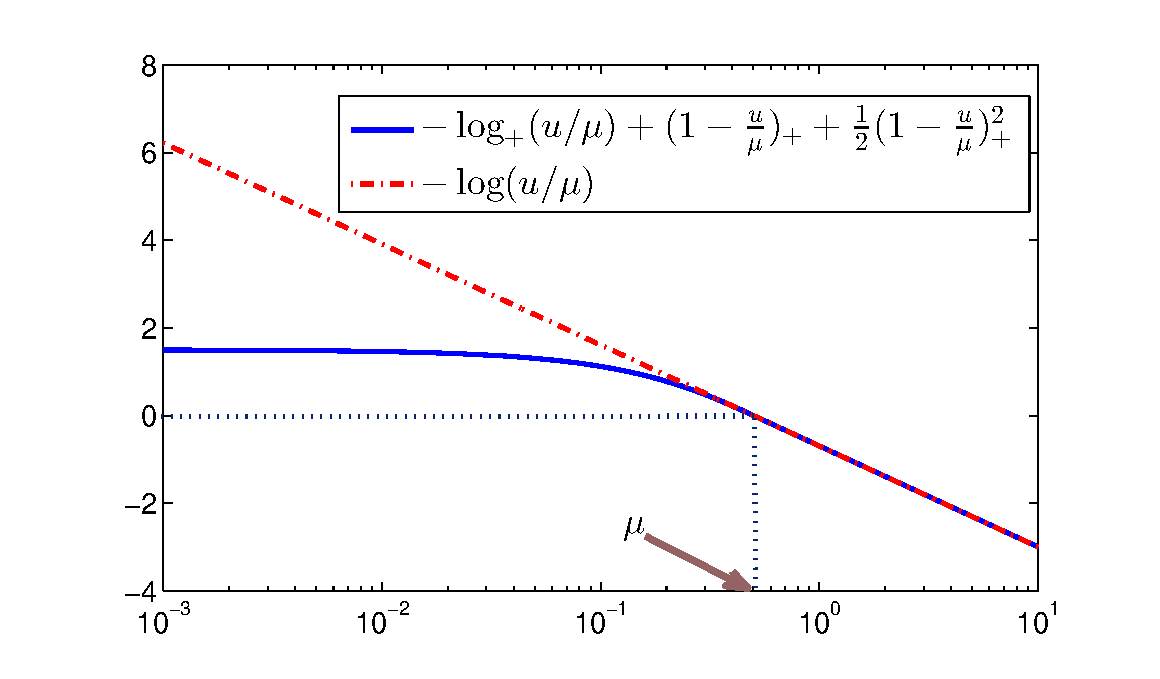
\includegraphics[width=0.8\textwidth]{./TeX_files/ell_and_ellbar.eps}
		\caption{The plot of the function $u\mapsto\bar\ell(u)$, used in the proof of
			\Cref{prop:2}, superposed on the plot of the function $u\mapsto\ell(u)=-\log u$.
			We see that the former is a strongly convex surrogate of the latter.}
		\label{fig:ell}
	\end{center}
\end{figure}
We repeat the proof of \Cref{maintheo1} with some small modifications. First of all, we replace the
function $\ell(u) = -\log(u)$ by the function
\begin{equation}\label{elBar}
\bar\ell(u) =
\begin{cases}
- \log(u/\mu), & \text{ if } u\ge \mu,\\
(1-\frac{u}{\mu})+\frac12(1-\frac{u}{\mu})^2, & \text{ if } u\in(0,\mu).
\end{cases}
\end{equation}
One easily checks that this function is twice continuously differentiable with a second
derivative satisfying $M^{-2}\le \bar\ell''(u)\le \mu^{-2}$ for every $u\in(0,M)$.
Furthermore, since $\bar\ell(u) = \ell(u/\mu)$ for every $u\ge \mu$, we have
$\bar L_n(\hat\bpi) = L_n(\hat\bpi)$, where we have used the notation $\bar L_n(\bpi)
= \frac1n\sum_{i=1}^n \bar\ell(f_{\bpi}(\bX_i))$. Therefore, similarly to \eqref{ineqOne},
we get
\begin{equation}\label{ineqOneb}
\frac{1}{n}\sum_{i=1}^n \bar\ell(f_{\hat\bpi}(\bX_i)) \leq
\frac{1}{n}\sum_{i=1}^n \bar\ell(f_{\bpi}(\bX_i)) -
\frac{1}{2M^2n}\|\bar\bfZ(\hat\bpi-\bpi)\|^2_2,
\end{equation}
for every $\bpi\in\Pi^*(\mu)$. Let us define $\bar \varphi(\bpi,\bx) = \bar\ell(f_{\bpi}(\bx))-
\int \bar\ell(f_{\bpi})f^*d\nu$ and $\bar\Phi_n(\bpi) = \frac1n\sum_{i=1}^n
\bar\varphi(\bpi,\bX_i)$. We have
\begin{align}
\int \bar\ell(f_{\hat\bpi})\,f^*d\nu
&\leq \int \bar\ell(f_{\bpi})\,f^*d\nu-\frac{1}{2M^2n}\|\bar\bfZ(\hat\bpi-\bpi)\|_2^2\nonumber\\
&+ \frac1n\sum_{i=1}^n \big(\varphi(\bpi,\bX_i)-\varphi(\hat\bpi,\bX_i)\big)\label{tempOraclIneqb}\\
&\leq \int \bar\ell(f_{\bpi})\,f^*d\nu-\frac{1}{2M^2n}\|\bar\bfZ(\hat\bpi-\bpi)\|_2^2\nonumber\\
&+\underbrace{\sup_{\bpi\in \Pi_n(0)}\|\nabla\bar\Phi_n(\bpi)\|_\infty}_{:=\xi_n} \|\hat\bpi-\bpi \|_1.
\end{align}\todos{modif: alignement}
Notice that $\bpi\in\Pi^*(\mu)$ implies that $\bar\ell(f_{\bpi}) = \log\mu-\log f_{\bpi}$
and that $\bar\ell(f_{\hat\bpi}) \ge  \log \mu-\log f_{\hat\bpi} -(\log\mu-\log f_{\hat\bpi})_+ $.
Therefore, along the lines of the proof of \eqref{boundDevTwo} (see, namely, \eqref{ineqa}),
we get
\begin{align}
\label{tempOraclIneqC}
\KL(f^*||f_{\hat\bpi})
&\leq \KL(f^*||f_{\bpi}) + \frac{2\xi_n^2M^2|J|}{\bar\kappa_{\hat\bSigma_n}(J,1)}
+\int_{\calX}(\log\mu-\log f_{\hat\bpi})_+f^*d\nu.
\end{align}
We can repeat now the arguments of \Cref{boundEmpProcess} with some minor modifications. First of all\todos{modif: changement de We first par first of all, cela permet un bon decalage}, we
rewrite $\xi_n$ as $\xi_n = \max_{l=1,\ldots,K} \xi_{l,n}$ with $\xi_{l,n} = \sup_{\bpi\in\Pi_n(0)}
|\partial_l \bar\Phi_n(\bpi)|$. One checks that the bounded difference inequality and the Efron-Stein
inequality can be applied with an additional factor 2, since for $F_l(\bfX) = \sup_{\bpi\in\Pi_n(0)}
|\partial_l \bar\Phi_n(\bpi)|$, we have
\begin{equation}
|F_l(\bfX)-F_l(\bfX')| \le \frac{2M}{n\mu} = \frac{2V}{n}.
\end{equation}
Therefore, for every $l\in[K]$, with probability larger than $1-(\delta/K)$, we have $\xi_{l,n}\le
\Ex[\xi_{l,n}]+ V(\frac{2\log(K/\delta)}{n})^{\nicefrac12}$ and $\var[\xi_n]\le (2V)^2/n$.
By the union bound, we obtain that with probability larger than $1-\delta$,
$\xi_{n}\le \max_l\Ex[\xi_{l,n}]+ V(\frac{2\log(K/\delta)}{n})^{\nicefrac12}$. Thus, to upper
bound $\Ex[\xi_{l,n}]$, we use the symmetrization argument:
\begin{align}
\Ex[\xi_{l,n}]
& \le 2\Ex\bigg[\sup_{\bpi\in\Pi_n(0)} \bigg|\frac1n\sum_{i=1}^n \epsilon_i
\bar\ell'(f_{\bpi}(\bX_i))f_l(\bX_i)\bigg|\bigg]\\
&\le 2M\Ex\bigg[\sup_{\bpi\in\Pi_n(0)} \bigg|\frac1n\sum_{i=1}^n \epsilon_i
\bar\ell'(f_{\bpi}(\bX_i))\bigg|\bigg]\\\
&\le \frac{2M}{\mu}\Ex\bigg[\bigg|\frac1n\sum_{i=1}^n \epsilon_i\bigg|\bigg]+
2M\Ex\bigg[\sup_{\bpi\in\Pi_n(0)} \bigg|\frac1n\sum_{i=1}^n \epsilon_i
[\bar\ell'(f_{\bpi}(\bX_i))-\bar\ell'(0)]\bigg|\bigg],
\end{align}
where the second inequality comes from \citep[Th.\ 11.5]{boucheron2013concentration}. \todos{deplacement de la citation en dehors de l'equation} Note that the function $\bar\ell'$, the derivative of $\bar\ell$ defined in \eqref{elBar},
is by construction Lipschitz with constant $1/\mu^2$. Therefore, in view of the contraction
principle,
\begin{align}
\Ex[\xi_{l,n}]
&\le \frac{2M}{\mu}\Ex\bigg[\bigg(\frac1n\sum_{i=1}^n \epsilon_i\bigg)^2\bigg]^{\nicefrac12}+
\frac{4M}{\mu^2}\Ex\bigg[\sup_{\bpi\in\Pi_n(0)} \frac1n\sum_{i=1}^n
\epsilon_if_{\bpi}(\bX_i)\bigg]\\
&\le \frac{2M}{\mu\sqrt{n}}+
\frac{4M}{\mu^2}\Ex\bigg[\sup_{k\in[K]} \frac1n\sum_{i=1}^n
\epsilon_i f_k(\bX_i)\bigg]\\
&\le \frac{2M}{\mu\sqrt{n}}+
\frac{8M^2}{\mu^2}\Big(\frac{\log K}{2n}\Big)^{\nicefrac12} \le \frac{2V^2(1+2\sqrt{2\log K})}{\sqrt{n}}.
\end{align}
As a consequence, we proved that with probability larger than $1-\delta$, we have
$\xi_n\le 8V^2(\frac{\log K}{n})^{\nicefrac12}$. This completes the proof of the first inequality.
In order to prove the second one, we simply change the way we have evaluated the term
$\int \bar\ell(f_{\hat\bpi})f^*$ in the left hand side of \eqref{tempOraclIneqb}. Since
$\bar\ell$ is strongly convex with a second order derivative bounded from below by $1/M^2$, we
have $\bar\ell(f_{\hat\bpi})\ge \bar\ell(f^*) + \bar\ell'(f^*)(f_{\hat\bpi}-f^*)+
\frac1{2M^2}(f_{\hat\bpi}-f^*)^2$. Since $f^*$ is always larger than $\mu$, the derivative
$\bar\ell'(f^*)$ equals $1/f^*$. Integrating over $\calX$, we get the second inequality of
the proposition.


%%%%%%%%%%%%%%%%%%%%% ================================================== %%%%%%%%%%%%%%%%%%%%%
\subsection{Auxiliary results}\label{ssec:auxiliary}
%%%%%%%%%%%%%%%%%%%%% ================================================== %%%%%%%%%%%%%%%%%%%%%


We start by a general convex result based on the strong convexity of the $-log$ function to
derive a bound on the estimated log-likelihood.
\begin{lemma}{}
	\label{convexlemma}
	Let us assume that $M =\max_{j\in[K]}\|f_j\|_\infty<\infty$. Then, for any $\bpi\in \BB^K_+$, it holds that
	\begin{equation}
	L_n(\hat\bpi) \le L_n(\bpi) -\frac1{2M^2n}\|\bar\bfZ(\hat\bpi-\bpi)\|_2^2.
	\end{equation}
\end{lemma}

\begin{proof}
	Recall that $\hat\bpi$ minimizes the function $L_n$ defined in \eqref{Phi} over $\Pi_n$. Furthermore,
	the function $u\mapsto \ell(u)$ is clearly strongly convex with a second order derivative bounded from below
	by $1/M^2$ over the set $u\in(0,M]$. Therefore, for every $\hat u\in(0,M]$, the function $\widetilde{\ell}$ given by:
	\begin{equation}
	\widetilde{\ell}(u)=\ell(u)-\frac{1}{2M^2}(\hat{u}-u)^2,\quad u\in(0,M],
	\end{equation}
	is convex.
	This implies that the mapping
	\begin{equation}
	\bpi\mapsto \widetilde L_n(\bpi) = L_n(\bpi)-\frac1{2 M^2 n}\|\bfZ(\hat\bpi-\bpi)\|_2^2
	\end{equation}
	is convex over the set $\bpi\in \BB^K_+$. This yields\footnote{We denote by $\partial g$ the sub-differential of a convex function $g$.}
	\begin{equation}
	\widetilde L_n(\bpi) -\widetilde L_n(\hat\bpi) \ge \sup_{\bv\in \partial\, \widetilde L_n(\hat\bpi)}\bv^\top (\bpi-\hat\bpi) ,\qquad \forall\bpi\in\BB^K_+.
	\end{equation}
	Using the Karush-Kuhn-Tucker conditions and the fact that $\hat\bpi$ minimizes $L_n$, we 
	get $\mathbf 0_K\in \partial\,L_n(\hat\bpi) = \partial\,\widetilde L_n(\hat\bpi)$. This 
	readily gives $\widetilde L_n(\bpi) -\widetilde L_n(\hat\bpi)\ge 0$, for any $\bpi\in\BB^K_+$. 
	The last step is to remark that $\bfZ(\hat\bpi-\bpi) = \bar\bfZ(\hat\bpi-\bpi)$, since both
	$\hat\bpi$ and $\bpi$ have entries summing to one.
\end{proof}

The core of our results lies in the following proposition which bound the deviations of the empirical process part.

\begin{prop}[Supremum of Empirical Process]
	\label{boundEmpProcess}
	For any $\bpi\in\BB^K_+$ and $\bx\in\calX$, define $\varphi(\pi,\bx) = \int (\log f_{\bpi})f^* -\log f_{\bpi}(\bx)$ and consider
	$\Phi_n(\bpi)=\frac1n\sum_{i=1}^n \varphi(\bpi,\bX_i)$. If $K\ge 2$, then for any $\delta \in (0,1)$, with probability at
	least $1-\delta$, we have
	\begin{equation}
	\zeta_n=\sup_{\bpi\in\Pi_n}\big\| \nabla \Phi_n(\bpi)\big\|_\infty \leq 8V^3\Big(\frac{\log(K/\delta)}{n}\Big)^{\nicefrac12}.
	\end{equation}
	Furthermore, we have $\Ex[\zeta_n]\le 4V^3\big(\frac{2\log(2K^2)}{n}\big)^{\nicefrac12}$ and $\var[\zeta_n]\le V^2/(2n)$.
\end{prop}
\begin{proof}
	To ease notation, let us denote $g_{\bpi,l}(x) = \frac{f_l(x)}{f_{\bpi}(x)}-
	\Ex\big[ \frac{f_l(\bX)}{f_{\bpi}(\bX)}\big]$ and
	\begin{equation}
	F(\mathbf X) = \sup_{\bpi\in\Pi_n}\big\| \nabla \Phi_n(\bpi)\big\|_\infty
	=\sup_{(\bpi,l)\in\Pi_n\times[K]}\Big|  \frac{1}{n}\sum_{i=1}^n g_{\bpi,l}(\bX_i) \Big|,
	\end{equation}
	where $\bfX=(\bX_1,\dots,\bX_n)$.  To derive a bound on $F$, we will use the McDiarmid concentration
	inequality that requires the bounded difference condition to hold for $F$. For some $i_0\in[n]$, let
	$\bfX'=(\bX_1,\dots,\bX'_{i_0},\dots,\bX_n)$  be a new sample obtained from $\bfX$ by modifying the
	$i_0$-th element $\bX_i$ and by leaving all the others unchanged. Then, we have
	\begin{align}
	F(\mathbf X)-F(\mathbf X')
	&= \sup_{(\bpi,l)\in\Pi_n\times[K]} \bigg|  \frac{1}{n}\sum_{i=1}^n g_{\bpi,l}\big(\bX_i\big) \bigg|-\sup_{(\bpi,l)\in\Pi\times[K]} \bigg|
	\frac{1}{n}\sum_{i=1}^n g_{\bpi,l}\big(\bX'_i\big) \bigg|\\
	&\leq \sup_{(\bpi,l)\in\Pi_n\times[K]}  \bigg|\frac{1}{n}\sum_{i=1}^n g_{\bpi,l}\big(\bX_i\big) - \frac{1}{n}\sum_{i=1}^n g_{\bpi,l}\big(\bX'_i\big)  \bigg|\\
	&=\sup_{(\bpi,l)\in\Pi_n\times[K]} \bigg| \frac{1}{n}\Big(g_{\bpi,l}\big(\bX_{i_0}\big) - g_{\bpi,l}\big(\bX'_{i_0}\big)\Big) \bigg|
	\leq \frac{V}{n},
	\end{align}
	where the last inequality is a direct consequence of assumption \eqref{densConst}. Therefore, using the McDiarmid concentration inequality recalled
	in \Cref{McDiarmid} below, we check that the inequality
	\begin{equation}
	\label{concIneqZ}
	F(\mathbf X) \leq \Ex(F(\mathbf X))+V\sqrt{\frac{\log(1/\delta)}{2n}}
	\end{equation}
	holds with probability at least $1-\delta$. Furthermore, in view of the Efron-Stein
	inequality, we have
	\begin{equation}
	\label{EfrStein}
	\var[\zeta_n] = \var[F(\mathbf X)] \leq \frac{V^2}{2n}.
	\end{equation}
	
	Let us denote $\calG:=\{(f_l/f_{\bpi})-1, (\bpi,l)\in\Pi_n\times [K]\}$ and $\mathfrak{R}_{n,q}(\calG)$ the Rademacher
	complexity of $\calG$ given by
	\begin{equation}
	\label{radCompl}
	\mathfrak{R}_{n}(\calG) = \Ex_{\epsilon}\bigg[ \sup_{(\bpi,l)\in\Pi_n\times[K]}\bigg| \frac{1}{n}\sum_{i=1}^n
	\epsilon_i\Big(\frac{f_l(\bX_i)}{f_{\bpi}(\bX_i)}-1\Big)\bigg| \bigg],
	\end{equation}
	with $\epsilon_1,\dots,\epsilon_n$ independent and identically distributed Rademacher random variables independent
	of $\bX_1,\dots,\bX_n$. Using the symmetrization inequality (see, for instance, Theorem~2.1 in~\cite{KoltBook2011})
	we have
	\begin{equation}
	\label{rademacher}
	\Ex[F(\mathbf X)] = \Ex[\zeta_n] \leq 2\Ex[\mathfrak{R}_{n}(\calG)].
	\end{equation}
	\begin{lemma}
		\label{boundRademComplex}
		The Rademacher complexity defined in \eqref{radCompl} satisfies
		\begin{equation}
		\mathfrak{R}_n(\calG) \leq  4V^3\sqrt{\frac{\log K}{n}}.
		\end{equation}
	\end{lemma}
	\begin{proof}
		The proof relies on the contraction principle of \cite{LedouxTal:91} that we recall in
		\Cref{sec:appendix_a} for the convenience. We apply this principle to the random variables
		$X_{i,(\bpi,l)}=f_{\bpi}(\bX_i)/f_l(\bX_i)-1$ and to the function $\psi(x) = (1+x)^{-1}-1$.
		Clearly $\psi$ is Lipschitz on
		$[\frac{1}{V}-1,V-1]$ with the Lipschitz constant equal to $V^2$ and $\psi(0)=0$. Therefore
		\begin{align}
		\mathfrak{R}_{n}(\calG)
		& \le  \Ex_{\epsilon}\bigg[ \sup_{(\bpi,l)} \frac{1}{n}\sum_{i=1}^n
		\epsilon_i\psi(\bX_{i,(\bpi,l)})\bigg]
		+\Ex_{\epsilon}\bigg[ \sup_{(\bpi,l)}\frac{1}{n}\sum_{i=1}^n
		\epsilon_i(-\psi)(\bX_{i,(\bpi,l)})\bigg]\nonumber\\
		&\leq 2V^2\Ex_{\epsilon}\bigg[ \sup_{(\bpi,l)\in\Pi_n\times[K]}\frac{1}{n}
		\sum_{i=1}^n \epsilon_i \bX_{i,(\bpi,l)} \bigg]\nonumber\\
		&= 2V^2 \Ex_{\epsilon}\bigg[ \sup_{(\bpi,l)\in\Pi_n\times[K]}\frac{1}{n}\sum_{i=1}^n \epsilon_i
		\bigg(\frac{f_{\bpi}(\bX_i)}{f_l(\bX_i)} -1\bigg) \bigg].
		\end{align}\todos{modif:supression des numero intermed.}
		Expanding $f_{\bpi}(\bX_i)$ we obtain
		\begin{align}
		\Ex_{\epsilon}\bigg[ \sup_{(\bpi,l)}\frac{1}{n}\sum_{i=1}^n \epsilon_i \bigg(\frac{f_{\bpi}(\bX_i)}{f_l(\bX_i)}
		-1\bigg) \bigg]
		&= \Ex_{\epsilon}\bigg[ \sup_{(\bpi,l)} \sum_{k=1}^K \frac{\pi_k}{n}\sum_{i=1}^n \epsilon_i
		\bigg(\frac{f_{k}(\bX_i)}{f_l(\bX_i)} -1\bigg)  \bigg]\nonumber\\
		&=\Ex_{\epsilon}\bigg[ \max_{k,l\in[K]} \frac{1}{n}\sum_{i=1}^n \epsilon_i
		\bigg(\frac{f_{k}(\bX_i)}{f_l(\bX_i)} -1\bigg) \bigg].
		\end{align}\todos{modif:supression des numero intermed.}
		We apply now \Cref{Hoeffding1} with $s= (k,l)$, $N = K^2$, $a=-V$, $b= V$ and $Y_{i,s} = \epsilon_i
		\big(\frac{f_{k}(\bX_i)}{f_l(\bX_i)} -1\big)$. This yields
		\begin{align}
		\Ex_{\epsilon}\bigg[ \max_{k,l\in[K]}  \frac{1}{n}\sum_{i=1}^n \epsilon_i
		\bigg(\frac{f_{k}(\bX_i)}{f_l(\bX_i)} -1\bigg) \bigg]
		\le 2V \Big(\frac{\log K^2}{2n}\Big)^{\nicefrac12}.
		\end{align}
		This completes the proof of the lemma.
	\end{proof}
	Combining inequalities (\ref{concIneqZ},\ref{rademacher}) and \Cref{boundRademComplex}, we get that the inequality
	\begin{equation}
	F(\bfX) \le 8V^3\Big(\frac{\log K}{n}\Big)^{\nicefrac12}+ V\Big(\frac{\log(1/\delta)}{2n}\Big)^{\nicefrac12}
	\end{equation}
	holds with probability at least $1-\delta$. Noticing that $V\ge 1$ and, for $K\ge 2$, $\delta\in(0,K^{-1/31})$
	we have $8\sqrt{\log K}+ \sqrt{(\nicefrac12){\log(1/\delta)}}\le 8\sqrt{\log(K/\delta)}$,
	we get the first claim of the proposition. The second claim is a direct consequence
	of \Cref{boundRademComplex} and \eqref{rademacher}.
\end{proof}

%%%%%%%%%%%%%%%%%%%%%%%%%%%%
\section[Proofs: Lower bounds]{Proof of the lower bound for nearly-$D$-sparse aggregation}\label{sec:proof-lower}
%%%%%%%%%%%%%%%%%%%%%%%%%%%%
We prove the minimax lower bound for estimation in Kullback-Leibler risk using 
the following slightly adapted version of Theorem~2.5 from \cite{tsybakov2009Nonparametric}. 
Throughout this section, we denote by $\lambda_{\min,\bSigma}(k)$ and $\lambda_{\max,\bSigma}(k)$,
respectively, the smallest and the largest eigenvalue of all $k\times k$ principal minors of 
the matrix $\bSigma$.
\begin{theorem}%(Theorem 2.5 from \cite{tsybakov2009Nonparametric})
	\label{tsy_main_theo_nonparam_est}
	For some integer $L\ge 4$ assume that
	$\calH_\calF(\gamma,D)$ contains $L$ elements $f_{\bpi^{(1)}},\dots,f_{\bpi^{(L)}}$
	satisfying the following two conditions.
	\vspace{-10pt}
	\begin{enumerate}[(i)]
		\item $\KL(f_{\bpi^{(j)}}||f_{\bpi^{(k)}})\geq2s>0$,  for all pairs $(j,k)$ such that $1\leq j<k\leq L$.
		\item For product densities $f_{\ell}^n$ defined on $\calX^n$ by $f_{\ell}^n(\bx_1,\ldots,\bx_n) =
		f_{\bpi^{(\ell)}}(\bx_1)\times\ldots\times f_{\bpi^{(\ell)}}(\bx_n)$ it holds 
		\begin{equation}
		\max_{\ell\in[L]} \KL(f_{\ell}^n||f_1^n) \leq \frac{\log L}{16}.
		\end{equation}
	\end{enumerate}
	\vspace{-10pt}
	Then
	\begin{equation}
	\inf_{\hat f}\sup_{f \in \calH_\calF(\gamma,D)}\Pb\!_{f}\big(\KL(f||\hat f)\geq s\big)\geq 0.17.
	\end{equation}
\end{theorem}
To establish the bound claimed in \Cref{theorem:lower_bound}, we will split the problem into two parts,
corresponding to the following two subsets of $\calH_\calF(\gamma,D)$
\begin{equation}
\begin{array}{ll}
\calH_\calF(0,D) &= \big\{f_{\bpi} : \bpi\in\BB^K_+ \text{ s.t. }\exists \, J\subset [K]
\text{ with } \|\bpi_{J^c}\|_1 = 0 \text{ and } |J|\le D\big\}, \\
\calH_\calF(\gamma,1) &= \big\{f_{\bpi} : \bpi\in\BB^K_+ \text{ s.t. } \pi_1 = 1-\gamma \text{ and } \sum_{j=2}^K\pi_j = \gamma \big\}.
\end{array}
\end{equation}\todos{modif: such that en s.t.}
We will show that over $\calH_\calF(0,D)$, we have a lower bound of order $\log(1+K/D)/n$ while over 
$\calH_\calF(\gamma,1)$, a lower bound of order 
$\big[\frac{\gamma^2}{n}\log\big(1+K/(\gamma\sqrt{n})\big)\big]^{\nicefrac12}$ holds true. Therefore, 
the lower bound  over $\calH_\calF(\gamma,D)$ is larger than the average of these bounds.

For any $M\geq 1$ and $k\in [M-1]$, let  $\Omega_k^M$ be the subset of $\{0,1\}^M$ defined by
\begin{equation}
\Omega_k^M := \Big \{\bomega \in \{0,1\}^M : \|\bomega\|_1=k \Big\}.
\end{equation}
Before starting, we remind here a version of the Varshamov-Gilbert lemma (see, for instance, \citep[Lemma 8.3]{RT11})
which will be helpful for deriving our lower bounds.
\begin{lemma}
	\label{rigollet8.3}
	Let $M\geq 4$ and $k\in[M/2]$ be two integers. Then there exist a subset $\Omega \subset \Omega_k^M$ and an absolute constant $C_1$
	such that
	\begin{equation}
	\|\bomega-\bomega'\|_1 \geq \frac{k+1}{4} \quad \forall \bomega,\bomega' \in \Omega \text{ \rm s.t. } \bomega \neq \bomega'
	\end{equation}
	and $L=|\Omega|$ satisfies $L\ge 4$ and
	\begin{equation}
	\log L  \geq C_1 k\log\Big(1+\frac{eM}{ k}\Big).
	\end{equation}
\end{lemma}
We will also use the following lemma that allows us to relate the KL-divergence $\KL(f_{\bpi}||f_{\bpi'})$ 
to the Euclidean distance between the weight vectors $\bpi$ and $\bpi'$. 
\begin{lemma}
	\label{lemma:KLboundsLT}
	If the dictionary $\calF$ satisfies the boundedness assumption~\eqref{densConst}, then for any
	$f_{\bpi}, f_{\bpi'}\in \calH_\calF(\gamma,D)$ we have
	\begin{equation}
	\frac{1}{2V^2M}\,\|\bSigma^{\nicefrac12}(\bpi'-\bpi)\|_2^2
	\leq \KL(f_{\bpi}||f_{\bpi'})
	\leq \frac{V^2}{2m}\,\|\bSigma^{\nicefrac12}(\bpi'-\bpi)\|_2^2.
	\end{equation}
\end{lemma}
\begin{proof}
	Using the Taylor expansion, one can check that for any $u\in[1/L,L]$, we
	have $(1-u)+ \frac{1}{2V^2}(u-1)^2 \leq -\log u \leq (1-u)+\frac{V^2}{2}(u-1)^2$.
	Therefore,
	\begin{equation}
	\frac{1}{2V^2}\int_{\calX}\Big(\frac{f_{\bpi'}}{f_{\bpi}}-1\Big)^2f_{\bpi}\,d\nu
	\leq \KL(f_{\bpi}||f_{\bpi'}) \leq \frac{V^2}{2}\int_{\calX}\Big(\frac{f_{\bpi'}}{f_{\bpi}}-1\Big)^2
	f_{\bpi}\,d\nu.
	\end{equation}
	Since $\calF$ satisfies the boundedness assumption, we get
	\begin{equation}
	\label{KLboundsLT}
	\frac{1}{2MV^2}\int_{\calX}\big(f_{\bpi'}-f_{\bpi}\big)^2d\nu
	\leq \KL(f_{\bpi}||f_{\bpi'}) \leq \frac{V^2}{2m}\int_{\calX}\big(f_{\bpi'}-f_{\bpi}\big)^2d\nu.
	\end{equation}
	The claim of the lemma follows from these inequalities and the fact that
	$\int_{\calX}\big(f_{\bpi'}-f_{\bpi}\big)^2d\nu = \|\bSigma^{\nicefrac12}(\bpi'-\bpi)\|_2^2$.
\end{proof}



\subsection{Lower bound on $\calH_\calF(0,D)$} % (fold)

\todos{mdif: suppression de here} We show that the lower bound ${(\nicefrac{D}n)\log(1+\nicefrac{e K}D)}
\wedge\big((\nicefrac1n){\log(1+\nicefrac{K}{\sqrt{n}})}\big)^{\nicefrac12}$ holds 
when we consider the worst case  error for $f^*$ belonging to the set $\calH_\calF(0,D)$. 
\begin{proposition}
	\label{prop:lower:1}
	If $\log(1+eK)\le  n$ then, for the constant
	\begin{equation}
	C_2=\frac{C_1 m\bar\kappa_{\bSigma}(2D,0)}{2^{9}V^2 M(C_1m\vee 4V^2\lambda_{\max,\bSigma}(2D))}
	\ge \frac{C_1 m\varkappa_*}{2^{9}V^2 M(C_1m\vee 4V^2\varkappa^*)},
	\end{equation} 
	we have
	\begin{equation}
	\small
	\inf_{\hat f}\sup_{f \in \calH_\calF(0,D)}\Pb\!_{f}\Bigg(\KL(f||\hat f)\geq
	C_2\,\frac{D\log(1+\frac{K}{D})}{n}\bigwedge\bigg(\frac{\log\big(1+\frac{K}{\sqrt{n}}\big)}{n}\bigg)^{\nicefrac12}\Bigg)
	\geq 0.17.
	\end{equation}\todos{modif: passé à frac et small}
\end{proposition}

\begin{proof}
	We assume that $D \leq \nicefrac{K}2$. The case $D> \nicefrac{K}2$ can be reduced to the
	case $D = \nicefrac{K}2$ by using the inclusion $\calH_\calF(0,\nicefrac{K}2)\subset \calH_\calF(0,D)$. Let us set $A_1 = 4\vee {16 V^2\lambda_{\max,\bSigma}(2D)}/{(C_1 m)}$ 
	and denote by $d$ the largest integer such that
	\begin{equation}\label{eqFvSxOa}
	d\le D\quad\text{and}\quad d^2\log\Big(1+\frac{e  K}{d}\Big)\le A_1 n.
	\end{equation}
	According to~\Cref{rigollet8.3}, there exists a subset
	$\Omega = \{\bomega^{(\ell)}:\ell\in[L]\}$ of  $\Omega_{d}^{K}$ of cardinality $L\ge 4$
	satisfying $\log L\geq {C_1 d}\log(1+{eK}/{d})$ such that for any pair of distinct 
	elements $\bomega^{(\ell)}$, $\bomega^{(\ell')}\in \Omega$ we have
	$\|\bomega^{(\ell)}-\bomega^{(\ell')}\|_1 \geq d/4$. Using these binary vectors $\bomega^{(\ell)}$, we define the set $\mathcal{D} =
	\{ \bpi^{(1)},\dots,\bpi^{(L)}\}\subset \BB_+^{K}$ as follows:
	\begin{equation}\label{eqFvSxTw}
	\bpi^{(1)}=\bomega^{(1)}/d,\quad
	\bpi^{(\ell)}=(1-\varepsilon)\bpi^{(1)}+\varepsilon \bomega^{(\ell)}/d,\quad \ell=2,\ldots,L.
	\end{equation}
	Clearly, for every $\varepsilon\in[0,1]$, the vectors $\bpi^{(\ell)}$ belong to  $\BB^K_+$.
	Furthermore, for any pair of distinct
	values $\ell,\ell'\in[L]$, we have $\|\bpi^{(\ell)}-\bpi^{(\ell')}\|_q^q = (\varepsilon/d)^q
	\|\bomega^{(\ell)}-\bomega^{(\ell')}\|_1\ge (\varepsilon/d)^qd/4$.  In view of~\Cref{lemma:KLboundsLT},
	this yields
	\begin{equation}\label{eqFvSxTh}
	\KL(f_{\bpi^{(\ell)}}||f_{\bpi^{(\ell')}})
	\geq \frac{\bar\kappa_{\bSigma}(2d,0)}{4V^2M d} \big{\|}\bpi^{(\ell)} - \bpi^{(\ell')}\big{\|}_1^2
	\geq \frac{\bar\kappa_{\bSigma}(2D,0)}{64V^2M}\times\frac{\varepsilon^2}{d}.
	\end{equation}
	Let us choose
	\begin{equation}
	\varepsilon^2 = \frac{d^2 \log(1+e  K/d)}{n A_1}.
	\end{equation}
	It follows from \eqref{eqFvSxOa} that $\varepsilon\le 1$. Inserting this value of
	$\varepsilon$ in \eqref{eqFvSxTh}, we get
	\begin{equation}
	\KL(f_{\bpi^{(\ell)}}||f_{\bpi^{(\ell')}}) \geq 2 C_2\,\frac{d\log(1+e  K/d)}{n}.
	\end{equation}
	This inequality \todos{modif: ajout inequality} shows that condition (i) of \Cref{tsy_main_theo_nonparam_est} is satisfied with
	$s= C_2\,(\nicefrac{d}{n})\log(1+e  K/d)$.  For the second condition of the same theorem, 
	we have
	\begin{align}
	\max_{\ell\in[L]}\KL(f^n_{\ell}||f^n_{1}) &= n\max_{\ell}\KL(f_{\bpi^{(\ell)}}||f_{\bpi^{(1)}})\\
	&\leq \frac{ n V^2\lambda_{\max,\bSigma}(2d)}{2m}\max_\ell \|\bpi^{(\ell)} - \bpi^{(1)}\|_2^2\\
	&\leq \frac{ n V^2\lambda_{\max,\bSigma}(2D)}{m} \times \frac{\varepsilon^2}{d},
	\end{align}
	since one can check that $\|\bpi^{(\ell)} - \bpi^{(1)}\|_2^2 \le (\varepsilon/d)^2 
	\|\bomega^{(\ell)}-\bomega^{(1)}\|_1\le 2\varepsilon^2/d$. Therefore, using the definition 
	of $\varepsilon$, we get
	\begin{align}
	\max_{\ell\in[L]}\KL(f^n_{\ell}||f^n_{1}) 
	&\le \frac{ n V^2\lambda_{\max,\bSigma}(2D)}{m}\times\frac{C_1dm\log(1+e  K/d)}
	{16 nV^2\lambda_{\max,\bSigma}(2D)}\\
	&= \frac{C_1d\log(1+e  K/d)}{16}\le \frac{\log L}{16}.
	\end{align}
	\Cref{tsy_main_theo_nonparam_est} implies that
	\begin{equation}\label{eqFvSxTwa}
	\inf_{\hat f}\sup_{f \in \calH_\calF(0,D)}\Pb\!_{f}\bigg(\KL(f||\hat f)\geq
	C_2\,\frac{d\log(1+e  K/d)}{n}\bigg)\geq 0.17.
	\end{equation}
	%Let us consider separately the following two cases: 
	%\begin{align}
	%\textbf{Case A}:&\quad \Big(\frac{D\log(1+eK/D)}{n}\Big)^2\le \frac{\log(1+K/\sqrt{n})}{n},\\
	%\textbf{Case B}:&\quad \Big(\frac{D\log(1+eK/D)}{n}\Big)^2> \frac{\log(1+K/\sqrt{n})}{n}.
	%\end{align}
	%In Case A, we get $\psi(D)\le \psi(\sqrt{n})$ where $\psi(x) = x\log(1+K/x)$ is an
	%increasing function on $[1,\infty)$. Therefore, we get $D\le \sqrt{n}$. This implies that
	%\begin{align}
	%\frac{D^2\log(1+eK/D)}{n} 
	%    &\le \Big(\frac{D\log(1+eK/D)}{n}\Big)^2\frac{n}{\log(1+eK/D)}\\
	%    &\le \frac{\log(1+K/\sqrt{n})}{n}\frac{n}{\log(1+eK/D)}\\ 
	%    &\le \frac{\log(1+K/D)}{\log(1+eK/D)}\le 1.
	%\end{align}
	%Thus, $d=D$  and the claim of the proposition follows from \eqref{eqFvSxTwa}. 
	%In case B, 
	We use the fact that $d$ is the largest integer satisfying 
	\eqref{eqFvSxOa}. Therefore, either $d+1>D$ or 
	\begin{equation}\label{eqFvSxTha}
	(d+1)^2\log\Big(1+\frac{e  K}{d+1}\Big)\le A_1 n.
	\end{equation}
	If $d\ge D$, then the claim of the proposition follows from \eqref{eqFvSxTwa}, since
	$d\log(1+eK/d)\ge D\log(1+eK/D)$. On the other hand, if \eqref{eqFvSxTha} is true, then
	\begin{align}
	d\log(1+eK/d) 
	&\ge \frac12 (d+1)\log(1+eK/(d+1))\nonumber \\
	&\ge \frac12 \big({A_1 n}{\log(1+eK/(d+1))}\big)^{\nicefrac12}.
	\end{align}
	In addition, $d^2\log(1+eK/d)\le A_1 n$ implies that $(d+1)^2 \le A_1 n$. Combining the last
	two inequalities, we get the inequality $d\log(1+eK/d)  \ge \nicefrac12 \big({A_1 n}{\log(1+eK/\sqrt{A_1n})}\big)^{\nicefrac12}\ge  \big({n}{\log(1+eK/\sqrt{n})}\big)^{\nicefrac12}$. 
	Therefore, in view of \eqref{eqFvSxTwa}, we get the claim of the proposition.
\end{proof}


\subsection{Lower bound on $\calH_\calF(\gamma,1)$} % (fold)

Next result shows that the lower bound ${\frac{\gamma^2}n\log\big(1+\frac{K}{\gamma\sqrt{n}}\big)}$ 
holds for the worst case error when $f^*$ belongs to the set $\calH_\calF(\gamma,1)$. 
\begin{proposition}\label{prop:lower:2}
	Assume that
	\begin{equation}
	\Big(\frac{\log(1+eK)}{n}\Big)^{\nicefrac12}\le 2\gamma.
	\end{equation}
	Then, for the constant $C_3 =
	\frac{C_1 m \bar\kappa_{\bSigma}(2D,0) }{2^{12}V^4 M\lambda_{\max,\bSigma}(2D)}$,
	it holds that
	\begin{equation}
	\inf_{\hat f}\sup_{f \in \calH_\calF(\gamma,1)}\Pb\!_{f}\bigg(\KL(f||\hat f)\geq
	C_3\,\Big\{{\frac{\gamma^2}n\log\Big(1+\frac{K}{\gamma\sqrt{n}}\Big)}\Big\}^{\nicefrac12}\bigg)\geq 0.17.
	\end{equation}
\end{proposition}


\begin{proof}
	Let $C>2$ be a constant the precise value of which will be specified later.
	Denote by  $d$ the largest integer satisfying
	\begin{equation}\label{eqFvSxFv}
	d\sqrt{\log(1+eK/d)} \leq C{\gamma\sqrt{n}}.
	\end{equation}
	Note that $d\ge 1$ in view of the condition $(\frac{\log(1+eK)}{n})^{\nicefrac12}\le 2\gamma$ of the 
	proposition. This readily implies that $d\leq C\gamma\sqrt{n}$ and, therefore, 
	\begin{equation}\label{eqFvSxSx}
	\frac{\gamma}{d} 
	\ge C^{-1}\Big\{{\frac1n\log\Big(1+\frac{eK}{C\gamma\sqrt{n}}\Big)}\Big\}^{\nicefrac12}
	\ge 2C^{-2}\Big\{{\frac1n\log\Big(1+\frac{K}{\gamma\sqrt{n}}\Big)}\Big\}^{\nicefrac12}.
	\end{equation}
	Let us first consider the case $d \leq (K-1)/2$. According to \Cref{rigollet8.3}, there 
	exists a subset $\Omega \subset \Omega_{d}^{K-1}$ of cardinality $L$ satisfying 
	$\log L\geq C_1\log\big(1+\frac{e(K-1)}{d}\big)$ and $\|\bomega^{(\ell)}-\bomega^{(\ell')}\|_1\geq d/4$
	for any pair of distinct elements $\bomega,\bomega'$ taken from $\Omega$. With these 
	binary vectors in hand, we define the set $\calD \subset \BB_+^K$ of cardinality $L$ as follows:
	\begin{equation}
	\calD = \Big\{\bpi = \big(1-\gamma,{\gamma}\bomega/{d}\big) : \quad\omega \in \Omega\Big\}.
	\end{equation}
	It is clear that all the vectors of $\calD$ belong to $\calH_\calF(\gamma,1)$. 
	Let us fix now an element of $\calD$ and denote it by $\bpi^1$, the corresponding element of
	$\Omega$ being denoted by $\bomega^1$. We have
	\begin{align}
	\max_{\bpi\in\calD}\KL(f^n_{\bpi}||f^n_{\bpi^1})
	&\leq \frac{nV^2}{2m}\max_{\bpi\in\calD} \|\bSigma^{\nicefrac12}(\bpi-\bpi^{1})\|_2^2 \\
	&\leq \frac{nV^2\lambda_{\max,\bSigma}(2d)\gamma^2}{2m d^2} \max_{\bomega\in\Omega}
	\|\bomega-\bomega^{1}\|_2^2\\
	&\leq \frac{nV^2\lambda_{\max,\bSigma}(2d)\gamma^2}{m d}. \label{eqKLlowerBoundInq}
	\end{align}
	The definition of $d$ yields $(d+1)\sqrt{\log(1+eK/(d+1))}> C\gamma\sqrt{n}$, which implies that
	\begin{align}
	\frac{\gamma^2}{d}
	&\leq 2(d+1)\frac{\gamma^2}{(d+1)^2}\nonumber\\
	&\leq 2(d+1)\frac{\log\big(1+eK/(d+1)\big)}{nC^2}\nonumber\\
	&\leq \frac{4d\log\big(1+e(K-1)/d\big)}{nC^2}.
	\end{align}
	Combined with \cref{eqKLlowerBoundInq}, this implies that
	\begin{align}
	\max_{\bpi\in\calD}\KL(f^n_{\bpi}||f^n_{\bpi^1})
	&\leq \frac{nV^2\lambda_{\max,\bSigma}(2d)}{m}\times \frac{4d\log\big(1+e(K-1)/d\big)}{nC^2}\\
	&= \frac{4V^2\lambda_{\max,\bSigma}(2d)}{m C^2}\times {d\log\big(1+e(K-1)/d\big)}.
	\end{align}
	Choosing%\footnote{One easily checks that this constant $C$ is always larger than $2$.}
	$$
	C^2 = 2\vee\frac{64 V^2\lambda_{\max,\bSigma}(2d)}{C_1 m}
	$$
	we get that $\max_{\bpi\in\calD}\KL(f^n_{\bpi}||f^n_{\bpi^1})\le \frac1{16} C_1{d\log\big(1+e(K-1)/d\big)}\le
	\frac{\log L}{16}$.
	
	Furthermore, for any $\bpi,\bpi'\in\calD$, in view of~\Cref{lemma:KLboundsLT} and \eqref{eqFvSxSx}, we have
	\begin{align}
	\KL(f_{\bpi} || f_{\bpi'}) &\geq \frac{\bar\kappa_{\bSigma}(2d,0)}{4V^2M d} \big{\|}\bpi - \bpi'\big{\|}_1^2
	=\frac{\bar\kappa_{\bSigma}(2d,0)\gamma^2}{4V^2M d^3} \|\bomega - \bomega'\big\|_1^2\\
	&\geq \frac{\bar\kappa_{\bSigma}(2d,0)}{64V^2M}\times \frac{\gamma^2}{d}\\
	&\geq \frac{\bar\kappa_{\bSigma}(2d,0)}{32V^2M C^2}\times 
	\Big\{{\frac{\gamma^2}n\log\Big(1+\frac{K}{\gamma\sqrt{n}}\Big)}\Big\}^{\nicefrac12}.
	\end{align}
	Since $\frac{\bar\kappa_{\bSigma}(2d,0)}{32V^2M C^2} = 2C_3$, this implies that 
	\Cref{tsy_main_theo_nonparam_est} can be applied, which leads to the inequality
	\begin{equation}
	\inf_{\hat f}\sup_{f \in \calH_\calF(\gamma,1)}\Pb\!_{f}\bigg(\KL(f||\hat f)\geq
	C_3\,\Big\{{\frac{\gamma^2}n\log\Big(1+\frac{K}{\gamma\sqrt{n}}\Big)}\Big\}^{\nicefrac12}\bigg)\geq 0.17.
	\end{equation}
	To complete the proof of the proposition, we have to consider the case $d > (K-1)/2$. In this case,
	we can repeat all the previous arguments for $d= K/2$ and get the desired inequality.
\end{proof}

\subsection{Lower bound holding for all densities} % (fold)

Now that we have lower bounds in probability for $\calH_\calF(0,D)$ and $\calH_\calF(\gamma,1)$, we can derive a lower bound in expectation for
$\calH_\calF(\gamma,D)$. In particular, to prove \Cref{theorem:lower_bound},
we will use the inequality
\begin{equation}\label{eqFvSxSev}
\calR\big(\calH_{\calF}(\gamma,D)\big)  \ge \inf_{\hat f}
\sup_{f^*\in \calH_\calF(0,D)\cup \calH_\calF(\gamma,1)} \Ex[\KL(f^*||\hat f)].
\end{equation}



\begin{proof}[Proof of \Cref{theorem:lower_bound}]
	To ease notation, let us define
	\begin{equation}
	\small
	r(n,K,\gamma,D) = \bigg[\frac{\gamma^2}{n}
	\log\bigg(1+\frac{K}{\gamma\sqrt{n}}\bigg)\bigg]^{\nicefrac12}
	+ \frac{D\log(1+K/D)}{n}\bigwedge \Big(\frac{\log(1+K/\sqrt{n})}{n}\Big)^{\nicefrac12}.
	\end{equation}\todos{modif: transformé en small}
	We first consider the case where the dominating term is the first one, that is 
	\begin{equation}\label{eqFvSxZO}
	\bigg[\frac{\gamma^2}{n} \log\bigg(1+\frac{K}{\gamma\sqrt{n}}\bigg)\bigg]^{\nicefrac12}
	\ge \frac{ 3 D\log(1+K/D)}{n}.
	\end{equation}
	On the one hand, since $D\ge 1$, we have
	\begin{equation}\label{eqFvSxZT}
	\frac{ 3D\log(1+K/D)}{n}\ge \frac{ \log(1+eK)}{n}.
	\end{equation}
	On the other hand, using the inequality $\log(1+x)\le x$, we get
	\begin{align}
	\bigg[\frac{\gamma^2}{n} \log\bigg(1+\frac{K}{\gamma\sqrt{n}}\bigg)\bigg]^{\nicefrac12}
	&\le \frac{\gamma}{\sqrt{n}}\bigg[\log(1+eK)+\log\bigg(1+\frac{1}{e^2\gamma^2n}\bigg)\bigg]^{\nicefrac12}\\
	&\le \gamma\bigg[\frac{\log(1+eK)}{n}\bigg]^{\nicefrac12}+\frac{\gamma}{\sqrt{n}}\bigg[\frac{1}{e^2\gamma^2n}\bigg]^{\nicefrac12}\\
	&\le \gamma\bigg[\frac{\log(1+eK)}{n}\bigg]^{\nicefrac12}+\frac{\log (1+eK)}{2n}.\label{eqFvSxZTh}
	\end{align}
	Combining \eqref{eqFvSxZO}, \eqref{eqFvSxZT} and \eqref{eqFvSxZTh}, we get
	\begin{equation}
	\Big(\frac{\log(1+eK)}{n}\Big)^{\nicefrac12}\le 2\gamma.
	\end{equation}
	This implies that we can apply \Cref{prop:lower:2}, which yields
	\begin{equation}
	\inf_{\hat f}\sup_{f \in \calH_\calF(\gamma,D)}\Pb\!_{f}\bigg(\KL(f||\hat f)\geq
	C_3\,\Big\{{\frac{\gamma^2}n\log\Big(1+\frac{K}{\gamma\sqrt{n}}\Big)}\Big\}^{\nicefrac12}\bigg)\geq 0.17.
	\end{equation}
	In view of \eqref{eqFvSxZO}, this implies that
	\begin{equation}\label{eqFvSxZFr}
	\inf_{\hat f}\sup_{f \in \calH_\calF(\gamma,D)}\Pb\!_{f}\bigg(\KL(f||\hat f)\geq
	\frac34C_3\,r(n,K,\gamma,D)\bigg)\geq 0.17.
	\end{equation}
	We now consider the second case, where the dominating term in the rate is the 
	second one, that is
	\begin{equation}\label{eqFvSxZFv}
	\bigg[\frac{\gamma^2}{n} \log\bigg(1+\frac{K}{\gamma\sqrt{n}}\bigg)\bigg]^{\nicefrac12}
	\le \frac{ 3 D\log(1+K/D)}{n}\bigwedge 
	\Big(\frac{\log(1+K/\sqrt{n})}{n}\Big)^{\nicefrac12}.
	\end{equation}
	In view of \Cref{prop:lower:1}, we have
	\begin{equation}
	\small
	\inf_{\hat f}\sup_{f \in \calH_\calF(\gamma,D)}\Pb\!_{f}\Bigg(\KL(f||\hat f)\geq
	C_2\,\frac{D\log(1+\frac{K}{D})}{n}\bigwedge\bigg(\frac{\log\big(1+\frac{K}{\sqrt{n}}\big)}{n}\bigg)^{\nicefrac12}\Bigg)
	\geq 0.17.
	\end{equation}\todos{modif: passé à frac et small}
	In view of \eqref{eqFvSxZFv}, we get
	\begin{equation}\label{eqFvSxZSx}
	\inf_{\hat f}\sup_{f \in \calH_\calF(\gamma,D)}\Pb\!_{f}\bigg(\KL(f||\hat f)\geq
	\frac14 C_2\,r(n,K,\gamma,D)\bigg)\geq 0.17.
	\end{equation}
	Thus, we have proved that $\log(1+eK)\le n$ implies that
	\begin{equation}
		\inf_{\hat f}\sup_{f \in \calH_\calF(\gamma,D)}\Pb\!_{f}\big(\KL(f||\hat f)\geq
	C_4\,r(n,K,\gamma,D)\big)\geq 0.17,
	\end{equation}\todos{modif: transformé en equation}
	for some constant $C_4>0$, whatever the relation
	between $\gamma$ and $D$. The desired lower bound follows now from the Tchebychev 
	inequality
	$\Ex\big[\KL(f||\hat f)\big]\ge C_4\,r(n,K,\gamma,D)
	\Pb\!_{f}\big(\KL(f||\hat f)\geq C_4\,r(n,K,\gamma,D)\big)$.
\end{proof}


\section*{Appendix A: Concentration inequalities} % (fold)
\label{sec:appendix_a}

This section contains some well-known results, which are recalled here for the sake of the self-containedness
of the paper.

\begin{theorem}\label{Hoeffding1}
	For each $s=1,\ldots,N$, let $Y_{1,s},\ldots,Y_{n,s}$ be $n$ independent and zero mean random variables such that
	for some real numbers $a,b$ we have $\Pb(Y_{i,s}\in[a,b])=1$ for all $i\in[n]$
	and $s\in[N]$. Then, we have
	\begin{align}
	\Ex\Big[\max_{s\in[N]} \frac1n\sum_{i=1}^n Y_{i,s}\Big]&\le (b-a)\Big(\frac{\log N}{2n}\Big)^{\nicefrac12},\\
	\Ex\Big[\max_{s\in[N]}\Big| \frac1n\sum_{i=1}^n Y_{i,s}\Big|\Big]&\le (b-a)\Big(\frac{\log(2N)}{2n}\Big)^{\nicefrac12}.
	\end{align}\todos{modif: tranformé en align}
\end{theorem}
\begin{proof}
	We denote $Z_s = \frac1n\sum_{i=1}^n Y_{i,s}$ for $s=1,\ldots, N$ and $Z_s = -\frac1n\sum_{i=1}^n Y_{i,s}$
	for $s=N+1,\ldots,2N$. For every $s\in[2N]$, the logarithmic moment generating function $\psi_s(\lambda) =
	\log \Ex[e^{\lambda Z_{s}}]$ satisfies
	\begin{equation}
	\psi_s(\lambda) =  \log \big(\prod_i \Ex[e^{\lambda Y_{i,s}/n}])
	= \sum_{i=1}^n \log  \Ex[e^{\lambda Y_{i,s}/n}] \le \frac{\lambda^2(b-a)^2}{8n},
	\end{equation}
	where the last inequality is a consequence of the Hoeffding lemma (see, for instance,  Lemma~2.2
	in~\citep{boucheron2013concentration}). This means that $Z_s$ is sub-Gaussian with variance-factor
	$\nu = {(b-a)^2}/{4n}$. Therefore, Theorem~2.5 from \citep{boucheron2013concentration}
	yields $\Ex[\max_s Z_s]\le \sqrt{2\nu\log(2N)}$, which completes the proof.
\end{proof}

We group and state together the bounded differences and the Efron-Stein inequalities (\cite{boucheron2013concentration},
Theorems~6.2 and 3.1, respectively).

\begin{theorem}\label{McDiarmid}
	Assume that a function f satisfies the bounded difference condition: there exist constants $c_i$, $i=1,\ldots,n$
	such that for all $i=1,\ldots, n$, all $X=(X_1,\dots,X_i,\dots,X_n)$ and $X'=(X_1,\dots,X'_i,\dots,X_n)$ where
	only the $i^{th}$ vector is changed
	\begin{equation}
	|f(X)-f(X')| \leq c_i.
	\end{equation}
	Denote
	\begin{equation}
	\nu = \sum_{i=1}^n c_i^2.
	\end{equation}
	Let $Z=f(X_1,\dots,X_n)$ where $X_i$ are independent. Then, for every $\delta\in(0,1)$,
	\begin{equation}
	\Pb\Big\{Z\le \Ex Z +\Big(\frac{\nu\log(1/\delta)}{2}\Big)^{\nicefrac12} \Big\} \geq 1-\delta,\qquad\text{and}\qquad \var[Z] \le \frac{\nu}{2}.
	\end{equation}
\end{theorem}
% section appendix_b_mcdiarmid_inequality (end)

%\section*{Appendix B: Contraction Principle} % (fold)
%\label{sec:appendix_b}
Next we state the contraction principle of \citep{LedouxTal:91}; a proof can be found in
(\cite{boucheron2013concentration}, Theorem 11.6).
\begin{theorem}
	Let $x_1,\dots,x_n$ be vectors whose real-valued components are indexed by $\bTau$,
	that is, $x_i=(x_{i,s})_{s\in\bTau}$. For each $i=1,\dots,n$ let $\varphi_i:\RR\rightarrow\RR$
	be a $1$-Lipschitz function such that $\varphi_i(0)=0$. Let $\epsilon_1,\dots,\epsilon_n$ be
	independent Rademacher random variables, and let $\Psi:[0,\infty) \rightarrow \RR$ be a
	non-decreasing convex function. Then
	\begin{align}
	\Ex \bigg[\Psi\bigg(\frac{1}{2}\sup_{s\in\bTau}\bigg|\sum_{i=1}^n\epsilon_i\varphi_i(x_{i,s})\bigg| \bigg) \bigg]
	&\leq
	\Ex \bigg[\Psi\bigg(\sup_{s\in\bTau}\bigg|\sum_{i=1}^n\epsilon_i x_{i,s}\bigg| \bigg) \bigg]\\
	\Ex \bigg[\Psi\bigg(\sup_{s\in\bTau}\sum_{i=1}^n\epsilon_i\varphi_i(x_{i,s})\bigg) \bigg]
	&\leq  \Ex \bigg[\Psi\bigg(\sup_{s\in\bTau}\sum_{i=1}^n\epsilon_i x_{i,s} \bigg) \bigg] .
	\end{align}
\end{theorem}
% section appendix (end)

%!TEX root = ../main.tex

\chapter[Experiments for the KL-aggregation]{Experimental Results for the KL-aggregation}
\minitoc
In this section we propose an efficient algorithm for performing the KL-aggregation (see \Cref{chap:kl_aggreg}) and describe its implementation. We also compare its performance with different alternative methods. For the sake of simplicity, the comparison with the other methods is done in the univariate case only. The implementation of our algorithm and its behavior are the same in the multivariate setting.

\section{Introduction}


Before anything else, we remind the reader the problem setting and the estimator considered. We observe $n$ independent random vectors $\bX_1,\ldots,\bX_n\in\calX$ drawn from a probability distribution $P^*$ that admits a density function $f^*$ with respect to the Lebesgue measure. Given a family of mixture components $f_1,\ldots,f_K$, we assumed that this unknown density is well approximated by a convex combination $f_{\bpi}$ of these components:
\begin{equation}
f_{\bpi}(\bx)=\sum_{j=1}^K\pi_j f_j(\bx), \quad \bpi \in \BB_+^K=\Big\{\bpi\in [0,1]^K: \sum_{j=1}^K\pi_j=1\Big\}.
\end{equation}
The component densities $\calF=\{f_j:j\in[K]\}$ are assumed to be given by previous experiments or expert knowledge. The problem of construction of this family is an open problem that we try to address in section ?\todos{en parler}. The objective of this chapter is to expose and study experimentally the algorithm implemented for computing the Maximum Likelihood Estimator (MLE), defined by
\begin{equation}
\label{MLE_2}
\hat\bpi \in \argmin_{\bpi\in \BB_+^K}\Big\{-\frac{1}{n}\sum_{i=1}^n\log f_{\bpi}(\bX_i)\Big\}.
\end{equation}
One can note that this problem is convex as the composition of $-\log$ and a linear function is convex. Furthermore, the feasible space is also convex. This problem can be solved via a Primal-Dual interior point method. But we opted for an approach based on the accelerated proximal gradient descent method because of its suitability to the problems in high-dimensions with sparsity assumption \citep{Beck:2009:FIS:1658360.1658364}.

\section{Implementation}
\label{mle_kl_estim_impl}
\begin{figure}[ht]
\begin{center}
\mybox{
\begin{minipage}{0.85\linewidth}
\begin{algorithmic}%\SetAlgoLined\tt\SetLine
\small
\STATE {\bfseries Input: $\bpi\in\RR^p$.} 
\STATE {\bfseries Output:} The projection $\bpi^{proj}$ of $\bpi$ onto the probability simplex.
\STATE {\tt 1: Sort $\bpi$ into $\bu:\,u_1\geq u_2 \geq\dots\geq u_p$.}
\STATE {\tt 2: Find $\rho=\max \{1\leq j\leq p:\, u_j+\frac{1}{j}(1-\sum_{i=1}^j u_i) > 0\}$.}
\STATE {\tt 3: Define $\lambda = \frac{1}{\rho}(1-\sum_{i=1}^{\rho} u_i)$.}
\STATE {\tt 4: Construct $\bpi^{proj}\,\textnormal{s.t.}\, \bpi^{proj}_i=\max\{\pi_i+\lambda,0\},\,i=1,\dots,p$.}
\end{algorithmic}
\end{minipage}}
   \caption{ Projection procedure onto the probability simplex}
   \label{algo:proj_simplex.}
\end{center}
\end{figure}


We can see that \cref{MLE_2} is equivalent to
\begin{equation}
\argmin_{\bpi\in\RR^K}\big\{-\frac{1}{n}\sum_{i=1}^n\log f_{\bpi}(\bX_i)+\chi_{\BB_+^K}(\bpi)\big\},
\end{equation}
where $\chi_{\BB_+^K}$ is the indicator function
\begin{equation*}
    \chi_{\BB_+^K}(\bpi) =
    \begin{cases}
      0, & \text{if } \bpi\in \BB_+^K,\\
      +\infty, & \text{otherwise} .
    \end{cases}
\end{equation*}
This problem can be decomposed into 
\begin{equation}
\label{general_min_pb_fista}
    \min_{\bpi}\big\{\ell(\bpi)+g(\bpi)\big\},
\end{equation}
where $\ell(\bpi) =-\frac{1}{n}\sum_{i=1}^n\log f_{\bpi}(\bX_i)$ and $g(\bpi)=\chi_{\BB_+^K}(\bpi)$. One can note that this problem is convex but not smooth since $\ell$ is differentiable but $g$ is not. One way to tackle this minimization is to consider the proximal operator
\begin{equation}
    \textnormal{prox}_{\lambda g}(\bpi) = \argmin_{\bu}\big\{g(\bu)+\frac{1}{2\lambda}\|\bu-\bpi\|^2_2\big\},
\end{equation}
where $\lambda > 0$ is a scale parameter for the function $g$. One can interpret $\textnormal{prox}_{\lambda g}(\bpi)$ as a point that compromises between minimizing $g$ and being near to $\bpi$. Note that in our context, $g(.)=\chi_{\BB_+^K}(.)$, therefore
\begin{align*}
    \textnormal{prox}_{\lambda g}(\bpi) &= \argmin_{\bu}\big\{\chi_{\BB_+^K}(\bu)+\frac{1}{2\lambda}\|\bu-\bpi\|^2_2\big\},\\
    &= \argmin_{\bu\in \BB_+^K}\big\{\|\bu-\bpi\|^2_2\big\},\\
    &= \bPi_{\BB_+^K}(\bpi)
\end{align*}
where $\bPi_{\BB_+^K}(\bpi)$ is the Euclidean projection of $\bpi$ into the probability simplex. The reader can find in \citep{Parikh:2014:PA:2693612.2693613} a detailed study of proximal algorithms. A particularly interesting procedure for our problem is the proximal gradient method that solves \cref{general_min_pb_fista}. This method is iterative and the $(k+1)^{th}$ step is
\begin{equation}
    \bpi^{k+1} := \textnormal{prox}_{\lambda^k g}(\bpi^k-\lambda^k\nabla f(\bpi^k)),
\end{equation}
where $\lambda^k > 0$ is a step size. This step size can be found via a line-search method \citep{Parikh:2014:PA:2693612.2693613}. However, if $\nabla f$ is $L$-Lipschitz, we can chose a fixed $\lambda^k\in (0,1/L)$. In this setting, one can show that this method converges with a rate of $\mathcal O(1/k)$. This rate is known to be sub-optimal. To improve this slow rate, accelerated versions of the proximal gradient method have been developed \citep{RePEc:cor:louvco:2007076,Beck:2009:FIS:1658360.1658364} that achieve optimal $\mathcal O(1/k^2)$ rate under the $L$-Lipschitz condition on $\nabla f$. These optimization methods rely on the proximal operator and Nesterov's accelerated gradient method \citep{Nesterov:1983wy}. A version of this accelerated method is
\begin{equation*}
    \begin{cases}
    \bxi^k &:= \bpi^k + \omega^k(\bpi^k-\bpi^{k-1}),\\
    \bpi^{k+1} &:= \textnormal{prox}_{\lambda^k g}(\bxi^k-\lambda^k\nabla f(\bxi^k)),
    \end{cases}
\end{equation*}
where $\omega^k$ is defined by $\omega^1 := 1$ and
\begin{equation*}
    \omega^k := \frac{2(\omega^{k-1}-1)}{1+\sqrt{1+(\omega^{k-1})^2}}.
\end{equation*}
This method has been coined Fast Iterative Shrinkage-Thresholding Algorithm (FISTA) in \citep{Beck:2009:FIS:1658360.1658364}. Our procedure is a special case of this algorithm that can be called ``Accelerated projected gradient descent'' since the proximal is the projection into $\BB_+^K$. A procedure for the projection onto the probability simplex can be found in \citep{Duchi:2008:EPL:1390156.1390191} and a simple proof in \citep{Wang13projectiononto}. The procedure for this projector is given in \Cref{algo:proj_simplex.}. Finally, the complete procedure for our algorithm is given in \Cref{fig:pi_fista}.

\begin{figure}[h]
\begin{center}
\mybox{
\begin{minipage}{0.85\linewidth}
\begin{algorithmic}[1]%\SetAlgoLined\tt\SetLine
\small
\STATE {\bfseries Input:} A gradient step $\lambda$.
\STATE {\bfseries Output:} parameter estimate $\hat\bpi$.
\STATE {\tt 1: Initialize $t_0=1$ and $\bpi_0=(1/K,\dots,1/K)$,}
\FOR{$k\geq 1,$ until convergence occurs, }
\STATE {(a) $\bpi_k = \bPi_{\BB_+^K}\big( \xi_k - \lambda \nabla f_{\xi_k}(\xi_k)\big)$,}
\STATE {(b) $t_{k+1}= \frac{1+\sqrt{1+4t_k^2}}{2}$,}
\STATE {(c) $\xi_{k+1} = \bpi_k + \big(\frac{t_k-1}{t_{k+1}}\big)(\bpi_k-\bpi_{k-1})$.}
\ENDFOR.
\end{algorithmic}
\end{minipage}}
   \caption{FISTA for the estimation of $\bpi$.}
   \label{fig:pi_fista}
\end{center}
\end{figure}
A nice property of this method is that it provides a sparse solution of this minimization problem 
which fits with our goal of selecting elements of the dictionary. General Primal-Dual interior 
points methods do not offer this feature.


\section{Alternative methods considered}

In this section we briefly describe several estimators of the density which are compared to our estimator. Note that although we used the algorithm EM in our experiments, we do not described it in this section since it is already done in \Cref{chap:intro}.
\subsection{SPADES}
A method combining the dictionary approach and the $\ell_1$-penalty (and, therefore, very close in spirit to our method) have been proposed by \citep{SPADES}. They studied the linear combinations (as opposed to convex combinations studied in the previous chapter) of functions $\{f_1,\dots,f_M\}$ with $f_j\in L_2(\RR^d)$, $j=1,\dots,M$:
\begin{equation}
    f_{\lambda}(x)=\sum_{j=1}^M\lambda_j f_j(x), \quad \lambda = (\lambda_1,\dots,\lambda_M)\in \RR^M.
\end{equation}
They suggested the following estimator $\hat \lambda$ called SPADES:
\begin{equation}
    \hat\lambda = \argmin_{\lambda \in \RR^M}\Big\{-\frac{2}{n}\sum_{i=1}^n f_{\lambda}(\bX_i) +\|f_{\lambda}\|^2 +2\sum_{j=1}^M\omega_j|\lambda_j|\Big\}.
\end{equation}
It could be interesting to include SPADES in our experimental evaluation, but we did not manage to find an easy-to-use implementation of it, and it turned out that our implementation was quite slow. Furthermore, the SPADES is conceptually close to the Adaptive Dantzig (AD) \citep{Bertin} procedure described in the next subsection. Therefore, we opted for excluding SPADES from our experiments but including AD.

\subsection{Adaptive Dantzig density estimation\label{ad_section}}

The Adaptive Dantzig estimator of a density has been introduced in \citep{Bertin}. This method is similar to ours as it constructs an estimator of the unknown density from a linear mixture of functions taken from a dictionary. The key idea of this estimator is to minimize the $\ell_1$-norm of the weight vector of the linear combination under an adaptive Dantzig constraint. This constraint comes from concentration inequalities. We recall here some material about the Dantzig selector. It has been introduced by \citep{candes2007} in the linear regression model
\begin{equation}
\label{ad_mod1}
  \bY = \bA \blambda_0 + \bepsilon
\end{equation}
where $\bY\in \RR^n$, $\bA$ is a $n$ by $M$ matrix, $\bepsilon \in \RR^n$ is the noise vector and $\blambda_0 \in \RR^M$ the unknown regression parameter to estimate. The Dantzig estimator is then defined as the solution of the problem
\begin{equation}
   \textnormal{minimize}\,  \|\blambda \|_1 \quad \text{subject to} \quad \| \bA^T(\bA\blambda-\bY)\|_{\infty} \leq \eta,
\end{equation}
where $\eta$ is a regularization parameter. Statistical properties of this estimator were established in \citep{bickel2009}. They considered the non-parametric regression framework
\begin{equation}
\label{ad_mod2}
    Y_i = f_0(x_i) + \epsilon_i, \quad i=1,\dots,n
\end{equation}
where $f$ is an unknown function, the design points $(x_i)_{i=1,\dots,n}$ are known and $(\epsilon_i)_{i=1,\dots,n}$ is a noise vector. One can estimate $f_0$ as a weighted sum $f_{\blambda_0}$ of elements of a dictionary $D=(\varphi_m)_{m=1,\dots,M}$
\begin{equation}
\label{linear_mix_density}
  f_{\blambda_0} = \sum_{i=1}^M\lambda_{0, m}\varphi_m.
\end{equation}
One easily checks that the model in \ref{ad_mod2} coincides with model in \cref{ad_mod1} if we choose as design matrix 
$\bA = (\varphi_m(x_i))$. The goal of \citep{Bertin} was to estimate an unknown density $f_0$ with respect to a known 
measure $dx$ on $\RR$ by using the observation of $n$-sample $X_1,\dots,X_n$ and to build a linear combination $f_{\lambda}$ 
of elements of the dictionary $D$ as in \cref{linear_mix_density}. It follows from the strong law of large numbers that 
$$
\hat\beta_m = \frac{1}{n}\sum_{i=1}^n\varphi_m(X_i)
$$ 
converges almost surely to the scalar product of $f_0$ and $\varphi_m$:
\begin{equation}
      \int \varphi_m(x)f_0(x)dx=\beta_{0,m},
\end{equation}
and the Gram matrix associated to the dictionary $D$
\begin{equation}
    G_{m,m'}=\int\varphi_m(x)\varphi_{m'}(x)dx \quad \text{with}\quad 1\leq m,m' \leq M.
\end{equation}
The scalar product of $f_{\blambda}$ and $\varphi_m$ is therefore
\begin{equation}
    \int\varphi_m(x)f_{\blambda}(x)dx = \sum_{m'=1}^M\lambda_{m'}\int\varphi_{m'}(x)\varphi_m(x)dx = (\bG\blambda)_m.
\end{equation}
The Dantzig estimate $\hat\blambda^D$ is then obtained by solving the following constrained minimization problem
\begin{equation*}
    \left\{
    \begin{array}{ll}
        \text{minimize}\, &\|\blambda\|_1 \\
        \text{subject to}\, &|(\bG\blambda)_m-\hat\beta_m|\leq \eta_{\gamma,m} \quad m\in \{1,\dots,M\},
    \end{array} \right.
\end{equation*}
where, for a constant $\gamma > 0$,
\begin{equation}
    \eta_{\gamma,m} = \sqrt{\frac{2\tilde\sigma_m^2\gamma\log{M}}{n}}+ \frac{2\|\varphi_m\|_{\infty}\gamma\log{M}}{3n},
\end{equation}
with
\begin{equation}
    \tilde\sigma_m^2 = \hat\sigma_m^2+2\|\varphi_m \|_{\infty}\sqrt{\frac{2\hat\sigma_m^2\gamma\log{M}}{n}}+ \frac{8\|\varphi_m\|_{\infty}^2\gamma\log{M}}{n},
\end{equation}
and
\begin{equation}
    \hat\sigma^2_m = \frac{1}{n(n-1)}\sum_{i=2}^n\sum_{j=1}^{i-1}(\varphi_m(X_i)-\varphi_m(X_j)).
\end{equation}
Note that $\eta_{\gamma,m}$ depends on the data which explains the name \textit{Adaptive Dantzig}. \citep{Bertin} derived the form of $\eta_{\gamma,m}$ from sharp concentration inequalities (see Theorem 1 of \citep{Bertin}). More precisely, if we consider $\blambda_0=(\lambda_{0,m})_{m=1,\dots,M}$ such that the projection of $f_0$ on the space spanned by $D$ is
\begin{equation}
    \textbf{P}_{D}f_0=\sum_{m=1}^M\lambda_{0,m}\varphi_m,
\end{equation}
then $(\bG\blambda_0)_m=\beta_{0,m}$ and the parameter $\eta_{\gamma,m}$ can be seen as the smallest quantity such that, for $\gamma > 1$, we have $|\beta_{0,m}-\hat\beta_m|\leq \eta_{\gamma,m}$ with high probability. Note that the assumption $\gamma > 1$ is an almost necessary condition to have a theoretical control on the quadratic error $\Ex\|\hat f^D-f_0 \|^2_2$. Therefore, we will follow the choice of $\gamma=1.01$ made by the authors in our experiments. The pseudo code of the procedure is given in \Cref{algo:ad_algo}. In what follows, the Adaptive Dantzig density estimator is noted $\hat f ^{AD}$ and the abbreviation AD is used in the plots.

\begin{figure}[H]
\begin{center}
\mybox{
\begin{minipage}{0.85\linewidth}
\begin{algorithmic}[1]
\small
\STATE {\bfseries Input:} A sample $\bX_1,\ldots,\bX_n\in\RR^p$ and the dictionary $D=(\varphi_m)_{m=1,\dots,M}$.
\STATE {\bfseries Output:} Dantzig density estimate $\hat f^{AD}=f_{\hat \blambda^{D}}$.
\STATE {\bfseries Init:} Set $\gamma=1.01$.
\STATE Compute $\hat\beta_m = \frac{1}{n}\sum_{i=1}^N\varphi_m(\bX_i)$.
\STATE Compute $\hat\sigma^2_m = \frac{1}{n(n-1)}\sum_{i=2}^n\sum_{j=1}^{i-1}(\varphi_m(\bX_i)-\varphi_m(\bX_j))^2$.
\STATE Compute $\tilde\sigma_m^2$.
\begin{equation}
    \tilde\sigma_m^2 = \hat\sigma_m^2+2\|\varphi_m\|_{\infty}\sqrt{\frac{2\hat\sigma_m^2\gamma\log{M}}{n}}+ \frac{8\|\varphi_m\|_{\infty}^2\gamma\log{M}}{n}.
\end{equation}
\STATE Compute $\eta_{\gamma,m}$
\begin{equation*}
    \eta_{\gamma,m} = \sqrt{\frac{2\tilde\sigma_m^2\gamma\log{M}}{n}}+ \frac{2\|\varphi_m\|_{\infty}\gamma\log{M}}{3n}.
\end{equation*}
\STATE Compute the coefficients $\hat\blambda^{D,\gamma}$ of the Dantzig estimate, $\hat\blambda^{D,\gamma}=\argmin_{\blambda\in\RR^M}\|\blambda \|_1$ such that $\blambda$ satisfies the Dantzig constraint
\begin{equation}
    \forall m \in \{1,\dots,m\}, \quad |(\bG\blambda)_m-\hat\beta_m|\leq \eta_{\gamma,m}.
\end{equation}
\STATE Compute the mixture density $f_{\hat\blambda^D}=\sum_{m=1}^M\hat\lambda_m^D \varphi_m$.
\end{algorithmic}
\end{minipage}
}
   \caption{Adaptive Dantzig density estimation procedure}
   \label{algo:ad_algo}
\end{center}
\end{figure}


\subsection{Kernel density estimation}

The kernel density estimator (KDE) is a well established non-parametric way of estimating the probability density function of a random variable. We will recall in this section some material about KDE.\\
Let $X_1,\dots,X_n$ be i.i.d. random variables drawn from an unknown probability density $f$ with respect to the Lebesgue measure on $\RR$. The kernel density estimator $\hat f_h $ is given by
\begin{equation}
  \hat f_h(x) \triangleq \frac{1}{nh}\sum_{i=1}^nK\Big(\frac{X_i-x}{h}\Big)
\end{equation}
where $K:\RR \rightarrow \RR$ and $\int K(u)du = 1$ is called a kernel and $h$ is the bandwidth. We used Gaussian kernel and three methods to select the bandwidth: Cross Validation, Scott's rule of thumb which is the default method in Scipy \citep{scipy} and the Sheather and Jones bandwidth selection procedure \citep{sheather_bdwth}.
\subsubsection{Methods based on minimizing the AMISE}
The most natural way to derive an estimator of the bandwidth would be to minimize the Mean Integrated Squared Error (MISE)
\begin{equation}
    \label{mise}
    \textnormal{MISE}(h) := \EE\Big[\int(\hat f_h(x)-f(x))^2dx \Big].
\end{equation}
Unfortunately, we can not rely on this quantity since $f$ is unavailable. However, we can derive the first two terms of the asymptotic expansion of the MISE (AMISE). When $n\rightarrow\infty$ and $h=h(n)\rightarrow 0$, and under regularity assumptions on $f$ and $K$, we have
\begin{equation}
\label{amise}
    \textnormal{AMISE}(h) = \frac{1}{nh}R(K) +\frac{h^4\sigma^4_K}{4}R(f''),
\end{equation}
where for an appropriate function $g$, 
$$
R(g)=\int g^2(x) dx\qquad\text{ and }\qquad\sigma_g^2=\int x^2g(x) dx.
$$ 
The reader can refer to the appendix of \citep{tsybakov2009Nonparametric} for a proof of this expansion. 
Setting the derivative w.r.t.\ $h$ of the right hand side of \cref{amise} to $0$, we see that a suitable estimate 
of the bandwidth would be the solution of
\begin{equation}
\label{amise_diff_sol}
    h = \bigg(\frac{R(K)}{\sigma_K^4R(f'')}\bigg)^{1/5}n^{-1/5}.
\end{equation}
However, this cannot be done directly since we do not know $R(f'')$.  In the special case where we consider that 
the kernels are Gaussian and the target density to be estimated is also a Gaussian with density $\phi_{(0,\sigma^2)}$, we have $R(\phi_{(0,\sigma^2)}''(x)) = 3/(8\sqrt{\pi}\sigma^5)$ and we can derive the Scott's rule of thumb in univariate case \citep{scott_multivariate_2015}
\begin{equation}
    \hat h = (4/3)^{1/5}\sigma n^{-1/5} \approx 1.06\hat\sigma n^{-1/5}.
\end{equation}
Without this assumption on the target density, we have to look deeper into the study of $R(f'')$. Several estimators of this quantity has been developed to circumvent this issue \citep{HallMarron87, sheatherj91, sheather_bdwth}. We will focus on a popular method from \citep{sheather_bdwth}. The authors constructed a kernel density estimator of $R(f'')$
\begin{equation}
\label{sj_est_f2}
    \hat S(\hat\alpha_2(h)) = \frac{1}{n(n-1)}(\hat\alpha_2(h))^{-5}\sum_{i=1}^n\sum_{j=1}^n\Phi^{(4)}\Big(\frac{X_i-X_j}{\hat\alpha_2(h)}\Big),
\end{equation}
where $\Phi^{(i)}$ is the $i^{th}$ derivative of the standard normal density. Note that $\hat\alpha_2(h)$ depends on $h$. An estimator of $\hat\alpha_2(h)$ can be built with specific properties on the diagonal elements of \cref{sj_est_f2}
\begin{equation}
\label{sj_alpha_2}
    \hat\alpha_2(h) = 1.357\big(\hat S(a)/\hat T(b)\big)^{1/7}h^{5/7},
\end{equation}
with
\begin{equation}
\label{sj_est_f3}
    \hat T(b) = -\frac{1}{n(n-1)}b^{-7}\sum_{i=1}^n\sum_{j=1}^n\Phi^{(6)}\Big(\frac{X_i-X_j}{b}\Big),
\end{equation}
and 
\begin{equation}
    a = 0.920\hat\lambda n^{-1/7}, \quad b= 0.912\hat\lambda n^{-1/9},
\end{equation}
where $\hat\lambda$ is the sample interquartile range. We will not go into the details of these expressions but it is worth mentioning that $\hat T(b)$ is a kernel density estimator of $R(f''')$. Therefore combining \cref{sj_est_f2}, \cref{sj_alpha_2} and \cref{sj_est_f3}, we can solve \cref{amise_diff_sol} over $h$ via a Newton-Raphson procedure. The algorithm is given in \Cref{algo:sj_method}.

\begin{figure}[H]
\begin{center}
\mybox{
\begin{minipage}{0.85\linewidth}
\begin{algorithmic}[1]
\small
\STATE {\bfseries Input:} A sample $\bX_1,\ldots,\bX_n\in\RR$.
\STATE {\bfseries Output:} A bandwidth estimator $\hat h$.
\STATE {\bfseries Init:} Set $a = 0.920\hat\lambda n^{-1/7}$ and $b= 0.912\hat\lambda n^{-1/9}$.
\STATE Compute 
\begin{equation}
    \hat T(b) = -\frac{1}{n(n-1)}b^{-7}\sum_{i=1}^n\sum_{j=1}^n\Phi^{(6)}\Big(\frac{X_i-X_j}{b}\Big).
\end{equation}
\STATE Compute
\begin{equation}
    \hat S(a) = \frac{1}{n(n-1)}a^{-5}\sum_{i=1}^n\sum_{j=1}^n\Phi^{(4)}\Big(\frac{X_i-X_j}{a}\Big)
\end{equation}
\STATE Define the function $\hat\alpha_2(h) = 1.357\big(\hat S(a)/\hat T(b)\big)^{1/7}h^{5/7}$.
\STATE Solve over $h$
\begin{equation}
h-\bigg(\frac{R(K)}{\sigma_K^4 \hat S(\hat\alpha_2(h))}\bigg)^{1/5} = 0.
\end{equation}
\end{algorithmic}
\end{minipage}
}
   \caption{Sheather and Jones bandwidth selection method.}
   \label{algo:sj_method}
\end{center}
\end{figure}
\subsubsection{Behavior of KDE in high dimension}
It is well known that the kernel density estimator performs badly in the high dimensional setting, \citep{stone1980} proved that the kernel density estimator of a $p$ times continuously differentiable density in dimension $d$ converges at most at the rate $n^{-p/(2p+d)}$. Therefore, for a given target error, the size of the sample must increase exponentially as the dimension increases. For a study of kernel density estimators in the high dimensional setting, see Chapter 7 of \citep{scott_multivariate_2015}. 

\section{Experimental Evaluation}

In order to carry out an experimental evaluation, we constructed a set of target densities with different shapes and recorded the performances of the estimators. We considered different density dictionaries. Finally we assessed the performance through the Kullback-Leibler divergence and the $L_2$ distance. All the experiments reported in this section were conducted in the univariate case.

\subsection{Dictionaries considered}

We did experiments with the following two dictionaries containing various types of densities.
\begin{enumerate}
\item The first dictionary, denoted by $D_{GL}$, is composed of Gaussian and Laplace densities. 
The Gaussian densities have their means in the set 
$\{0, 0.2, 0.4, 0.6, 0.8, 1\}$ and their variances in $\{0.001, 0.01, 0.1, 1\}$. The Laplace densities have their 
means in $\{0, 0.2, 0.4, 0.6, 0.8, 1\}$ and their scales in $\{0.05, 0.1, 0.2, 0.5, 1\}$. Therefore, 
the dictionary $D_{GL}$ has 54 elements. The plots of these
functions are depicted in \Cref{fig:dict}.

\begin{figure}[h]
\centering
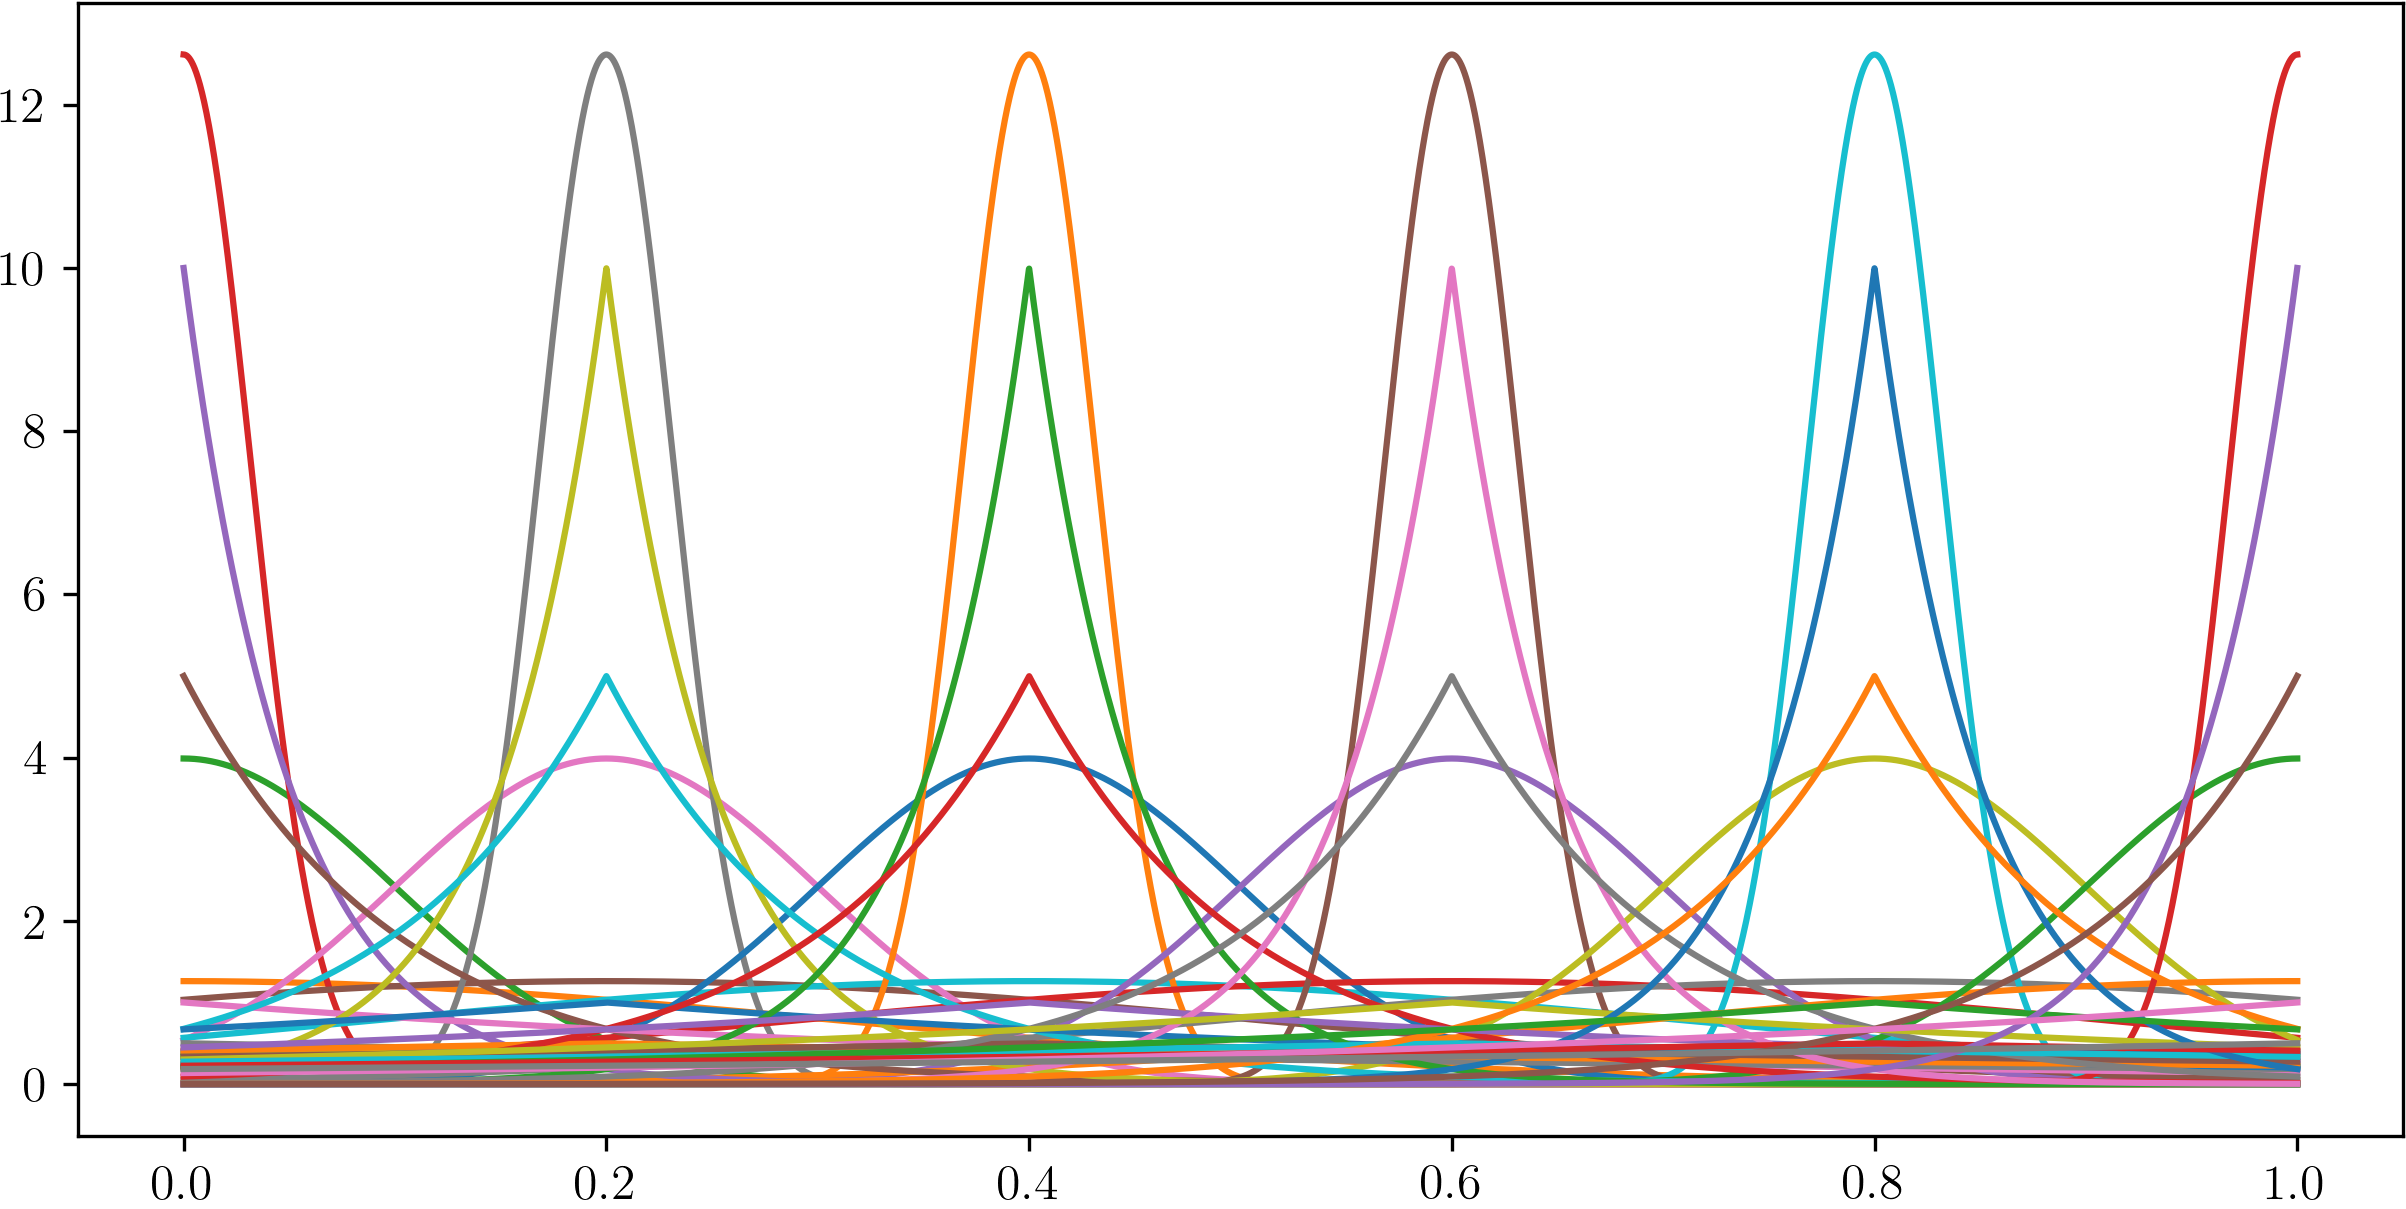
\includegraphics[width=1\textwidth]{TeX_files/lapl_gauss_dict.png}
\caption{$D_{GL}$, set of Gaussian and Laplace densities.}
\label{fig:dict}
\end{figure}
%\item Union of Fourier and Haar aud Gaussians ?
\item The second dictionary, denoted by $D_{GLU}$, is obtained by enriching
the first dictionary $D_{GL}$ by the set of $10$ uniform densities on the intervals 
$(i, i+0.1)$, $i\in \{0, 0.1,\dots,0.9\}$. This dictionary $D_{GLU}$ has 64 elements.
\end{enumerate}
A table of the dictionary $D_{GL}$ (and $D_{GLU}$ with the uniform densities) can be found in \Cref{table:densities_DGLU}.

\subsection{Densities considered}
We considered 5 target densities corresponding to 5 different scenarios. The $1^{st}$ and $2^{nd}$ will asses the performance of our method on uniform based densities, the $3^{rd}$ and $4^{th}$ on dictionary based density. The last one is a complex density made from elements which are not in the dictionary that we will consider.
\begin{enumerate}
\item{$f_{\textnormal{unif}}$:} A uniform density on $[0,1]$.
\item{$f_{\textnormal{rect}}$:} A mixture of uniform densities on subintervals. This density is called ``Rectangular'':
\begin{equation}
    f_{\textnormal{rect}}=\frac{10}{7}\b1_{[0,1/5]}+\frac{5}{7}\b1_{[1/5,2/5]}+
    \frac{10}{7}\b1_{[2/5,3/5]}+\frac{10}{7}\b1_{[4/5,1]}.
\end{equation}
\item{$f_{\textnormal{gauss}}$:} A mixture of 5 Gaussian densities taken from the dictionary $D_{GL}$ equally centered in $[0,1]$ with same variance:
\begin{equation}
    f_{\textnormal{gauss}}=\sum_{k=1}^5 0.2f_{k} \quad \text{with}\quad f_k=\varphi_{(k/5,0.001)}.
\end{equation}

\item{$f_{\textnormal{gauss-lapl}}$:} A mixture of 5 Gaussian and Laplace densities taken from the dictionary $D_{GL}$ with different variances and scales:
%(multivariate_normal(0.2, 10**(-3)))
%(multivariate_normal(0.6, 10**(-3)))
%(multivariate_normal(0, 10**(-2)))
%(laplace(0.4,0.2))
%(laplace(0.8,0.1))
\begin{equation}
\begin{array}{ll}
f_{\textnormal{gauss-lapl}}=0.2\big(&\varphi_{(0 ,10^{-2})} + \varphi_{(0.2,10^{-3})}+\varphi_{(0.6,10^{-3})}\\
    &+\text{\small Lapl}_{(0.4,0.2)}+\text{\small Lapl}_{(0.8,0.1)} \big).
\end{array}
\end{equation}
\item{$f_{\textnormal{ext}}$:} A mixture of Gaussian and Laplace densities taken from another dictionary $D_{out}$:
%append(multivariate_normal(0.1, 5*10**(-3)))
%append(multivariate_normal(0.65, 10**(-3)))
%append(multivariate_normal(0.9, 10**(-2)))
%append(laplace(0.5, 0.08))
%append(laplace(0.2, 0.07))
%append(laplace(0.75, 0.05))

\begin{equation}
    f_{\textnormal{ext}}=\sum_{k=1}^7 \frac{1}{7}f_{k} \quad \text{with}\quad f_k\in D_{out}.
\end{equation}
\end{enumerate}
These target densities are plotted in \Cref{fig:target_densities}.
\begin{figure}[h]
\center
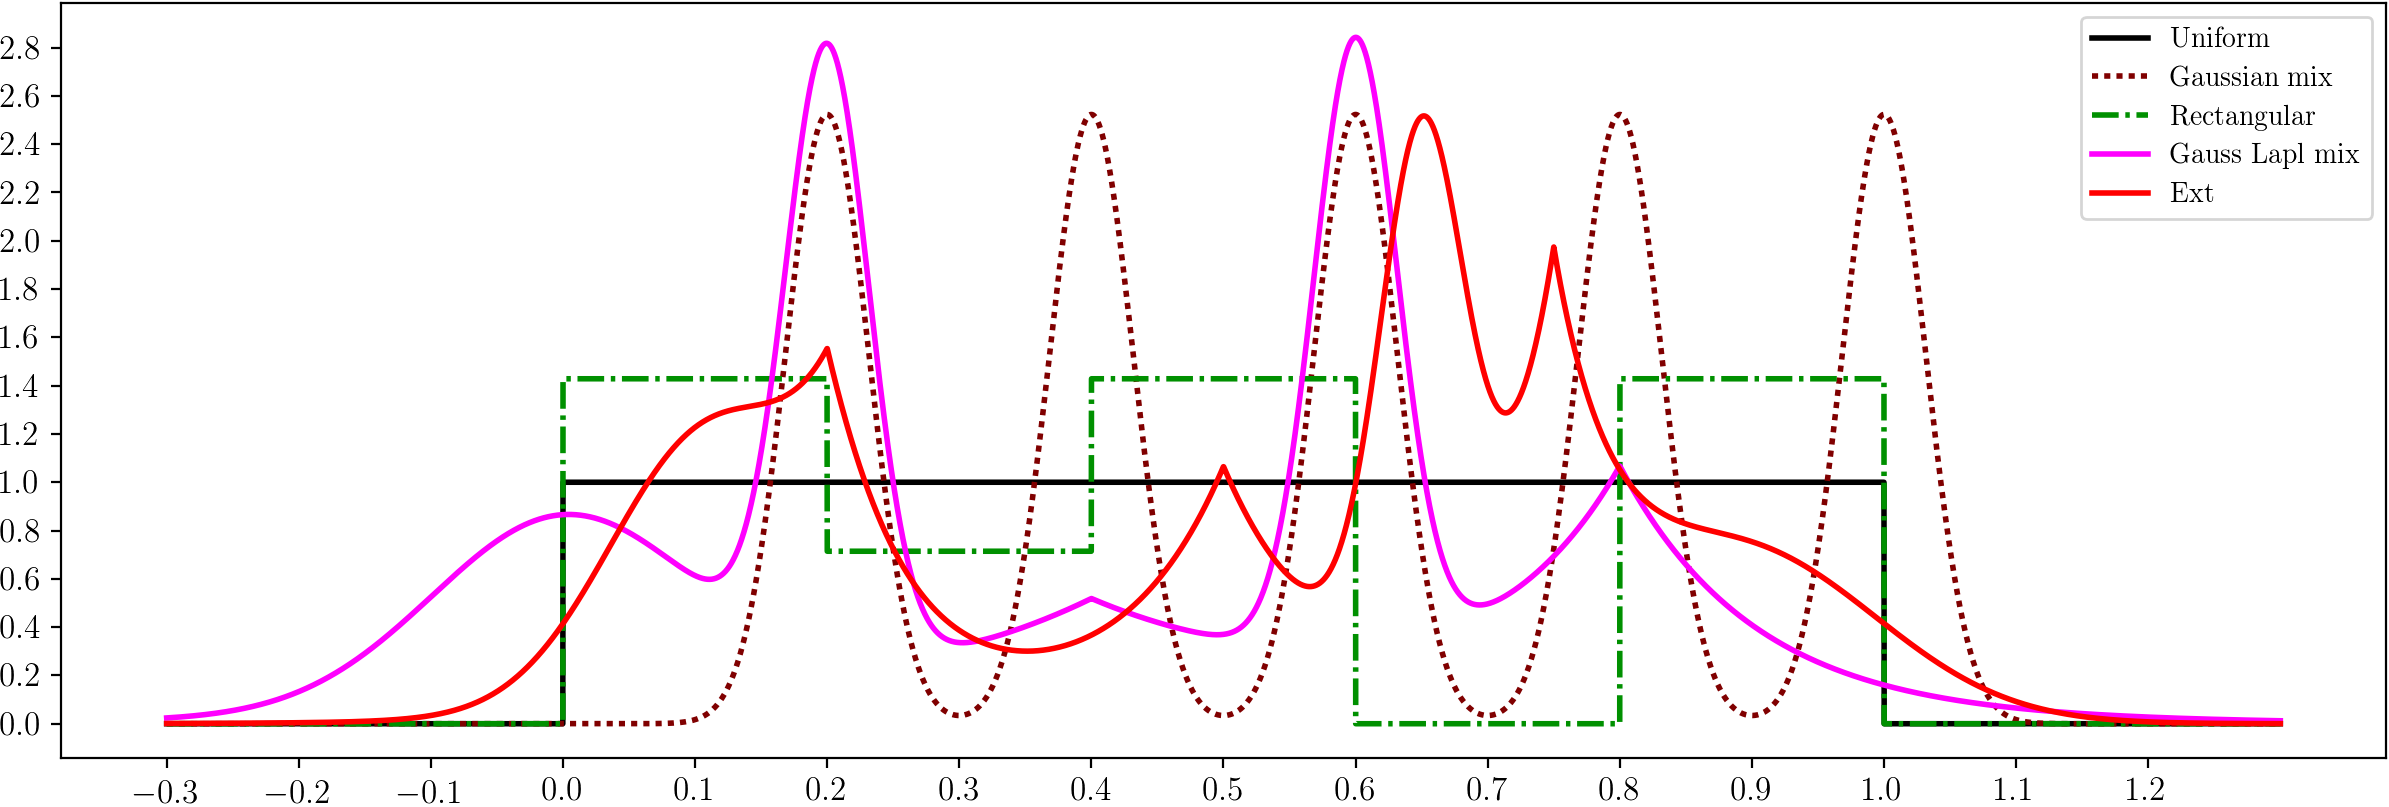
\includegraphics[width=1.1\textwidth]{TeX_files/densities_f_star.png}
\caption{Five target densities considered.}
\label{fig:target_densities}
\end{figure}

\subsection{Discussion of the results}

In the numerical experiments reported in this section, the dictionaries used for the Adaptive Dantzig 
and the Maximum likelihood density estimators are $D_{GL}$ and $D_{GLU}$. Note that the AD is the direct 
competitor of the MLE as both methods rely on a dictionary. However, in order to get a broader insight of
what is going on, we also compared these dictionary based methods with other commonly used density 
estimators such as the EM algorithm on Gaussian mixtures with a model selection performed by the BIC 
criterion and Kernel Density Estimators (KDE). In the plots, KDE refers to the kernel density estimate 
with Scott's rule as chosen by default in the Python library Scipy, KDE-SJ refers to the KDE with the 
Sheather-Jones bandwidth selector and KDE CV refers to the KDE with bandwidth selected via cross-validation. 
The two latter were implemented by ourselves. 

For each scenario of the target density, $f_{\textnormal{unif}}$, $f_{\textnormal{rect}}$, 
$f_{\textnormal{gauss}}$, $f_{\textnormal{gauss-lapl}}$, $f_{\textnormal{ext}}$ and for each sample size $N$  
with $N\in\{100, 500, 1000\}$, we ran 200 simulations. The boxplots of the errors are plotted in 
\Cref{fig:res_ext_L2_GL}-\Cref{fig:res_ext_KL_GLU}. The running times of different arguments are 
depicted in \Cref{fig:res_times}. A rapid observation is that the performance of the MLE is good both 
in Kullback-Leibler and $L_2$ losses, and it outperforms in all considered scenarios the 
AD estimator. This is true both in terms of statistical accuracy and computational complexity. 
The comparison with the other estimation methods is more subtle, and requires a closer look
to the results.

\subsubsection{Mis-specification bias}

Obviously, the densities $f_{\textnormal{unif}}$, $f_{\textnormal{rect}}$ and $f_{\textnormal{ext}}$ 
were not built with elements in the dictionary $D_{GL}$. In other terms, they do not lie in the convex hull
of the dictionary $D_{GL}$. Furthermore, they can be hardly approximated by convex combinations of functions
from $D_{GL}$. Therefore, it is clear that whatever the dictionary based approach we use, it will have a 
significant bias due to the ``model mis-specification''. 


%Uniform, rect, ext
\begin{figure}
\center
    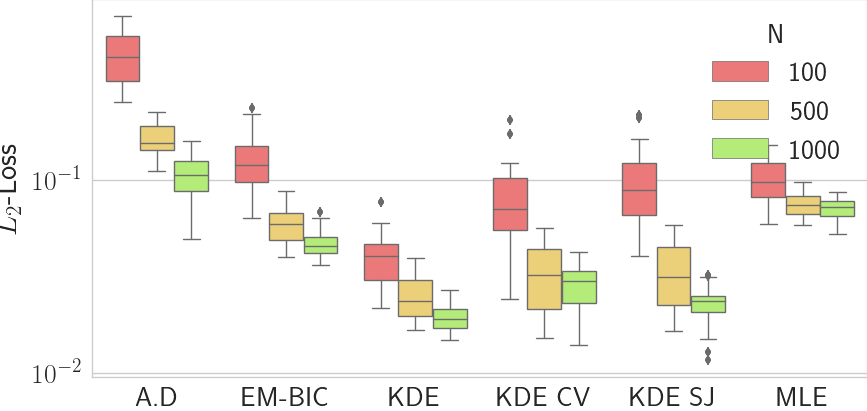
\includegraphics[width=0.8\textwidth]{./TeX_files/res_uniform_L2_GL.png}
    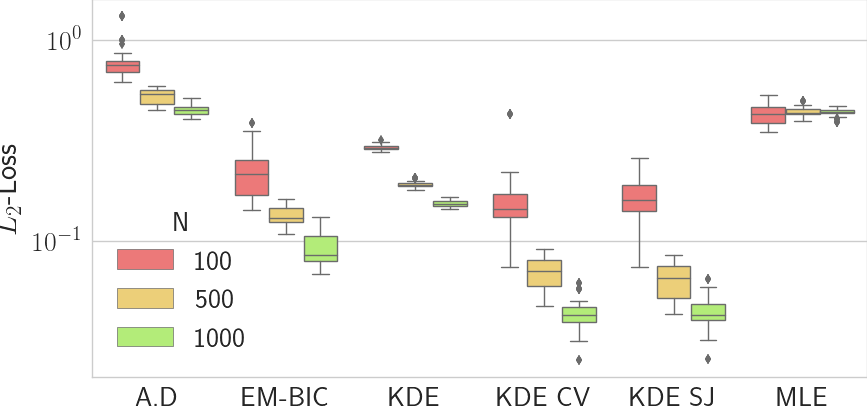
\includegraphics[width=0.8\textwidth]{./TeX_files/res_rect_L2_GL.png}
    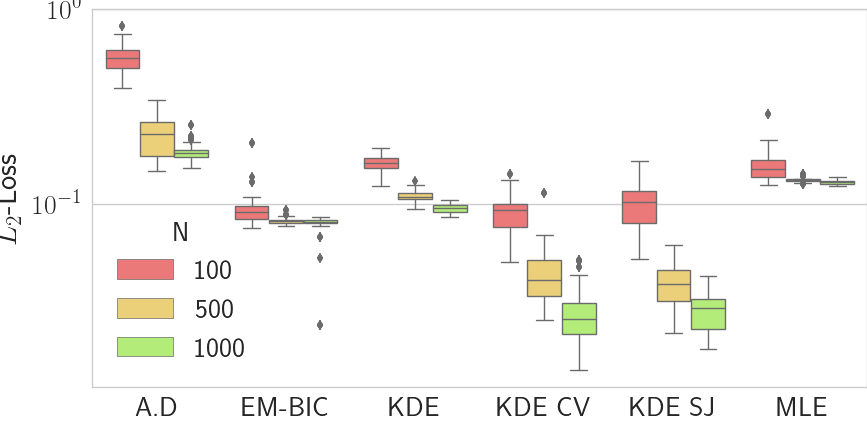
\includegraphics[width=0.8\textwidth]{./TeX_files/res_lapl_gauss_not_dict_L2_GL.png}
    \caption{Results with $f_{\textnormal{unif}}$ (upper panel), $f_{\textnormal{rect}}$ 
    (middle panel) and $f_{\textnormal{ext}}$ (lower panel) in $L2$ loss with $D_{GL}$.}
    \label{fig:res_ext_L2_GL}
\end{figure}

Since the cardinality of the dictionary is chosen
independently of the sample size $n$, this bias term is constant across different values of $n$. This is 
exactly what we observe in \Cref{fig:res_ext_L2_GL}. Such methods as the EM-BIC or various versions of KDE
have an $L_2$ error that decreases significantly when the sample size increases, whereas the AD and, especially, 
the MLE show only a slight improvement of the error. This is a strong indication of the fact that
the bias of the methods AD and MLE substantially dominates the bias, when the true density is chosen from 
the set $\{f_{\textnormal{unif}},\,f_{\textnormal{rect}},\,f_{\textnormal{ext}}\}$. Thus, the apparently
poor behavior of the MLE as compared to the EM-BIC and the KDE is not a surprise and, more importantly,
it is not caused by the method of estimation itself but rather by the inappropriate choice of the
dictionary.

Note that in all the experiments, the conclusions drawn from the error bars corresponding to the 
$L_2$-error can be drawn from the error bars corresponding to the KL-error. 

\begin{figure}
\center
    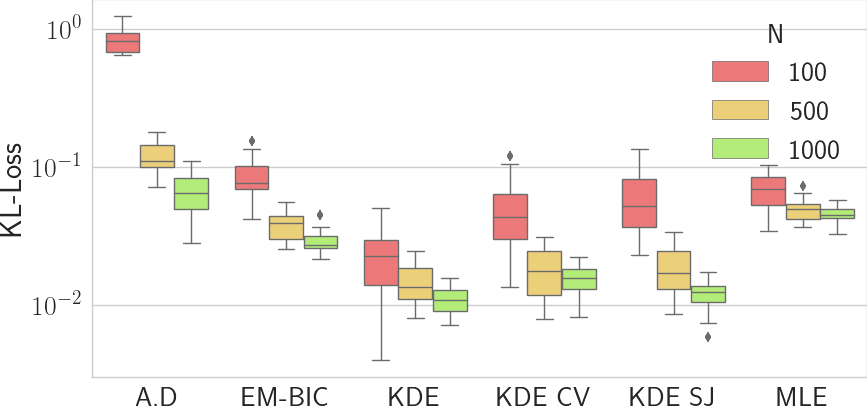
\includegraphics[width=0.8\textwidth]{./TeX_files/res_uniform_KL_GL.png}
    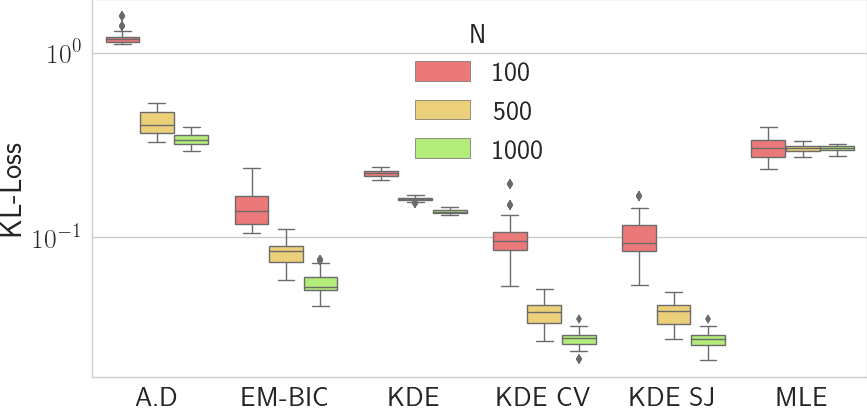
\includegraphics[width=0.8\textwidth]{./TeX_files/res_rect_KL_GL.png}
    \includegraphics[width=0.8\textwidth]{./TeX_files/res_lapl_gauss_not_dict_KL_GL.png}
    \caption{Results with $f_{\textnormal{unif}}$ (upper panel), $f_{\textnormal{rect}}$ 
    (middle panel) and $f_{\textnormal{ext}}$ (lower panel) in KL loss with $D_{GL}$.}
    \label{fig:res_ext_KL_GL}
\end{figure}

\subsubsection{Assessing estimation error}

While for the three densities discussed in the foregoing paragraph the bias was largely dominating 
the variance, the situation is reversed for the densities $f_{\textnormal{gauss}}$ and 
$f_{\textnormal{gauss-lapl}}$. Both of them belong to the convex hull of the dictionary 
$D_{GL}$, which implies that the mis-specification bias vanishes. Therefore, the error
is mostly dominated by the estimation variance. This explains why for these two densities
the MLE has the smallest error, both in $L_2$ and KL loss (see \Cref{fig:res_lapl_gauss_L2_GL} 
and \Cref{fig:res_lapl_gauss_KL_GL}). Interestingly, the second best is EM-BIC, which performs 
better than the AD. Note that the default KDE in Scipy \citep{scipy} with Scott's rule 
presents poor results in these scenarios. This observation should come to mind of the 
practitioner when applying kernel density estimators with default package setting. 

One can also remark that the error of the MLE when estimating $f_{\textnormal{gauss}}$
is smaller than the one of estimating $f_{\textnormal{gauss-lapl}}$. This is perfectly
in line with the theory developed in previous chapter, telling that the variance term
is proportional to the sparsity index. In these examples, the sparsity index of 
$f_{\textnormal{gauss-lapl}}$ is larger than that of $f_{\textnormal{gauss}}$.

%gauss
\begin{figure}
\center
    \includegraphics[width=0.8\textwidth]{./TeX_files/res_gauss_L2_GL.png}
    \includegraphics[width=0.8\textwidth]{./TeX_files/res_lapl_gauss_L2_GL.png}
    \caption{Results with $f_{\textnormal{gauss}}$ (upper panel) and $f_{\textnormal{gauss-lapl}}$ 
    (lower panel) in $L_2$ loss with $D_{GL}$.}
    \label{fig:res_lapl_gauss_L2_GL}
\end{figure}

\begin{figure}
\center
    \includegraphics[width=0.8\textwidth]{./TeX_files/res_gauss_KL_GL.png}
    \includegraphics[width=0.8\textwidth]{./TeX_files/res_lapl_gauss_KL_GL.png}
    \caption{Results with $f_{\textnormal{gauss}}$ (upper panel) and $f_{\textnormal{gauss-lapl}}$ 
    (lower panel) in KL loss with $D_{GL}$.}
    \label{fig:res_lapl_gauss_KL_GL}
\end{figure}


\subsubsection{Impact of the choice of the dictionary \label{dict_dglu_sect}}

The discussion of the foregoing paragraphs demonstrates the importance of the choice of the dictionary.
The purpose of the additional experiments conducted with the same target densities but with a larger dictionary, $D_{GLU}$,
is to further illustrate this importance and to show that the size of the dictionary does not significantly impact 
the quality of estimation\footnote{It certainly does impact the running time}.

The inclusion of  $10$ uniform densities on $(0,0.1),\dots,(0.9,1)$ to the dictionary $D_{GL}$ removes the mis-specification
bias in the case of a uniform and rectangular densities, and reduces it in the case of $f_{\textnormal{ext}}$.
The results are plotted in \Cref{fig:res_gauss_L2_GLU} and \Cref{fig:res_gauss_KL_GLU}. 
We can see that the MLE becomes generally the best estimator when the density is uniform or rectangular. 
It is still slightly worse than the KDE with data-driven bandwidths for estimating $f_{\textnormal{ext}}$.
 \begin{figure}
\center
    \includegraphics[width=0.8\textwidth]{./TeX_files/res_uniform_L2_GLU.png}
    \includegraphics[width=0.8\textwidth]{./TeX_files/res_rect_L2_GLU.png}
    \includegraphics[width=0.8\textwidth]{./TeX_files/res_lapl_gauss_not_dict_L2_GLU.png}
    \caption{Results with $f_{\textnormal{unif}}$ (upper panel), $f_{\textnormal{rect}}$ 
    (middle panel) and $f_{\textnormal{ext}}$ (lower panel) in $L_2$ loss with $D_{GLU}$.}
    \label{fig:res_gauss_L2_GLU}
\end{figure}
Finally, the results for the densities $f_{\textnormal{gauss}}$ and $f_{\textnormal{gauss-lapl}}$
plotted on \Cref{fig:res_ext_L2_GLU} and \Cref{fig:res_ext_KL_GLU} confirm that
adding new elements to the dictionary (even if they are ``useless'') do not deteriorate
the quality of estimation. The $\ell_1$-constraint allow us to avoid the overfitting. 
\begin{figure}
\center
    \includegraphics[width=0.8\textwidth]{./TeX_files/res_gauss_L2_GLU.png}
    \includegraphics[width=0.8\textwidth]{./TeX_files/res_lapl_gauss_L2_GLU.png}
    \caption{Results with $f_{\textnormal{gauss}}$ (upper panel) and $f_{\textnormal{gauss-lapl}}$ 
    (lower panel) in $L2$ loss with $D_{GLU}$.}
    \label{fig:res_ext_L2_GLU}
\end{figure}

\subsubsection{Comparison of weights estimated by AD and MLE}

A closer look on the estimated weights by AD and MLE gives us knowledge on the behavior of these estimators. We considered the full dictionary $D_{GLU}$ and we provided a table of the indexes of components of this dictionary in \Cref{table:densities_DGLU}. We plotted the estimated weights of the true components of $f_{\textnormal{gauss}}$ and $f_{\textnormal{gauss-lapl}}$ in \Cref{fig:weights_gauss_real_indexes} and \Cref{fig:weights_gauss_laplace_real_indexes}. The MLE estimates correctly the real weights of $f_{\textnormal{gauss}}$ and most of the weights of $f_{\textnormal{gauss-lapl}}$. We recall the reader that those weights were set to $0.2$. However, AD did not succeed to estimate correctly these weights. It turns out that AD gave importance on components that overlap the true densities of the mixture as shown in \Cref{fig:weights_gauss_and_laplace_unif_indexes} with the uniform components. Both AD and MLE provide sparse estimators, this can be seen by looking at components not used in the dictionary (see \Cref{fig:weights_gauss_and_laplace_other_indexes}). As a matter of fact, the estimated weight vector by AD is more sparse that MLE, but AD is more prone to be influenced by overlapping densities.

\begin{figure}
\center
    \includegraphics[width=0.8\textwidth]{./TeX_files/weight_f_gauss_real_comp_N_500.png}
    \includegraphics[width=0.8\textwidth]{./TeX_files/weight_f_gauss_real_comp_N_1000.png}
    \caption{Estimated weights of the components of $f_{\textnormal{gauss}}$, with $N=500$ (upper panel) and $N=1000$
    (lower panel).}
    \label{fig:weights_gauss_real_indexes}
\end{figure}
\begin{figure}
\center
    \includegraphics[width=0.8\textwidth]{./TeX_files/weight_f_gauss_unif_comp_N_1000.png}
    \includegraphics[width=0.8\textwidth]{./TeX_files/weight_f_gauss_laplace_unif_comp_N_1000.png}
    \caption{Estimated weights of uniform components of the dictionary for 
    $f_{\textnormal{gauss}}$ (upper panel) and $f_{\textnormal{gauss-lapl}}$ (lower panel) with $N=1000$.}
    \label{fig:weights_gauss_and_laplace_unif_indexes}
\end{figure}

\begin{figure}
\center
    \includegraphics[width=0.8\textwidth]{./TeX_files/weight_f_gauss_laplace_real_comp_N_500.png}
    \includegraphics[width=0.8\textwidth]{./TeX_files/weight_f_gauss_laplace_real_comp_N_1000.png}
    \caption{Estimated weights of the components of $f_{\textnormal{gauss-lapl}}$, with $N=500$ (upper panel) and $N=1000$
    (lower panel).}
    \label{fig:weights_gauss_laplace_real_indexes}
\end{figure}
\begin{figure}
\center
    \includegraphics[width=0.8\textwidth]{./TeX_files/weight_f_gauss_and_laplace_other_comp_N_1000.png}
    \caption{Estimated weights of non-used components of the dictionary for  $f_{\textnormal{gauss}}$ (upper panel) and $f_{\textnormal{gauss-lapl}}$ (lower panel), with $N=1000$.}
    \label{fig:weights_gauss_and_laplace_other_indexes}
\end{figure}

\begin{figure}
\center
\begin{tabular}{|c|l|c|l|c|l|}
\hline
0 & Normal( 0 , 1 ) &22 & Normal( 1 , 0.01 ) &44 & Laplace( 0.8 , 0.05 ) \\ \hline
1 & Normal( 0 , 0.1 ) &23 & Normal( 1 , 0.001 ) &45 & Laplace( 0.8 , 0.1 ) \\ \hline
2 & Normal( 0 , 0.01 ) &24 & Laplace( 0 , 0.05 ) &46 & Laplace( 0.8 , 0.2 ) \\ \hline
3 & Normal( 0 , 0.001 ) &25 & Laplace( 0 , 0.1 ) &47 & Laplace( 0.8 , 0.5 ) \\ \hline
4 & Normal( 0.2 , 1 ) &26 & Laplace( 0 , 0.2 ) &48 & Laplace( 0.8 , 1 ) \\ \hline
5 & Normal( 0.2 , 0.1 ) &27 & Laplace( 0 , 0.5 ) &49 & Laplace( 1 , 0.05 ) \\ \hline
6 & Normal( 0.2 , 0.01 ) &28 & Laplace( 0 , 1 ) &50 & Laplace( 1 , 0.1 ) \\ \hline
7 & Normal( 0.2 , 0.001 ) &29 & Laplace( 0.2 , 0.05 ) &51 & Laplace( 1 , 0.2 ) \\ \hline
8 & Normal( 0.4 , 1 ) &30 & Laplace( 0.2 , 0.1 ) &52 & Laplace( 1 , 0.5 ) \\ \hline
9 & Normal( 0.4 , 0.1 ) &31 & Laplace( 0.2 , 0.2 ) &53 & Laplace( 1 , 1 ) \\ \hline
10 & Normal( 0.4 , 0.01 ) &32 & Laplace( 0.2 , 0.5 )&54 & Uniform( 0.0 , 0.1 ) \\ \hline
11 & Normal( 0.4 , 0.001 ) &33 & Laplace( 0.2 , 1 )&55 & Uniform( 0.1 , 0.2 ) \\ \hline
12 & Normal( 0.6 , 1 ) &34 & Laplace( 0.4 , 0.05 )&56 & Uniform( 0.2 , 0.3 ) \\ \hline
13 & Normal( 0.6 , 0.1 ) &35 & Laplace( 0.4 , 0.1 )&57 & Uniform( 0.3 , 0.4 ) \\ \hline
14 & Normal( 0.6 , 0.01 ) &36 & Laplace( 0.4 , 0.2 )&58 & Uniform( 0.4 , 0.5 ) \\ \hline
15 & Normal( 0.6 , 0.001 ) &37 & Laplace( 0.4 , 0.5 )&59 & Uniform( 0.5 , 0.6 ) \\ \hline
16 & Normal( 0.8 , 1 ) &38 & Laplace( 0.4 , 1 )&60 & Uniform( 0.6 , 0.7 ) \\ \hline
17 & Normal( 0.8 , 0.1 ) &39 & Laplace( 0.6 , 0.05 )&61 & Uniform( 0.7 , 0.8 ) \\ \hline
18 & Normal( 0.8 , 0.01 ) &40 & Laplace( 0.6 , 0.1 )&62 & Uniform( 0.8 , 0.9 ) \\ \hline
19 & Normal( 0.8 , 0.001 ) &41 & Laplace( 0.6 , 0.2 )&63 & Uniform( 0.9 , 1.0 ) \\ \hline
20 & Normal( 1 , 1 ) &42 & Laplace( 0.6 , 0.5 )& &   \\ \hline
21 & Normal( 1 , 0.1 ) &43 & Laplace( 0.6 , 1 )& &   \\ \hline
\end{tabular}
\caption{Indexes of components of the dictionary $D_{GL}$ and $D_{GLU}$ }
\label{table:densities_DGLU}
\end{figure}

\subsubsection{Concluding remarks} 

To conclude, the performance of the MLE method in these simulations is promising to achieve a 
good mixture density estimate. In addition, the computational efficiency of the MLE displayed in 
\Cref{fig:res_times} makes it highly attractive for performing density estimation. Our algorithm 
was coded in Python with some elements accelerated with the Just-In-Time (JIT) compiler Numba \citep{numba}. 
Compared to compiled optimized versions of KDE and EM from Scipy and Scikit-Learn\citep{scikit-learn}, 
we are confident that the computation time of our algorithm can be further decreased. Another important 
point is in the case of high dimensional data, KDE and EM+BIC methods are known to present poor 
performance. Our method needs the computation of the matrix $(f_j(X_i))_{(i,j)\in [N]\times [K]}$ 
which might consume a lot of memory. Some techniques such as a Mini-batch approach can help. 
Furthermore, at the light of the results in the uniform and rectangular case, the choice of the 
dictionary is a cornerstone in density estimation. The size of the dictionary should be chosen 
by considering both statistical arguments and computational limitations.


\begin{figure}
\center
    \includegraphics[width=0.8\textwidth]{./TeX_files/res_uniform_KL_GLU.png}
    \includegraphics[width=0.8\textwidth]{./TeX_files/res_rect_KL_GLU.png}
    \includegraphics[width=0.8\textwidth]{./TeX_files/res_lapl_gauss_not_dict_KL_GLU.png}
    \caption{Results with $f_{\textnormal{unif}}$ (upper panel), $f_{\textnormal{rect}}$ 
    (middle panel) and $f_{\textnormal{ext}}$ (lower panel) in KL loss with $D_{GLU}$.}
    \label{fig:res_gauss_KL_GLU}
\end{figure}   
%lapl_gauss
\begin{figure}
\center
    \includegraphics[width=0.8\textwidth]{./TeX_files/res_gauss_KL_GLU.png}
    \includegraphics[width=0.8\textwidth]{./TeX_files/res_lapl_gauss_KL_GLU.png}
    \caption{Results with $f_{\textnormal{gauss}}$ (upper panel) and $f_{\textnormal{gauss-lapl}}$ 
    (lower panel) in KL loss with $D_{GLU}$.}
    \label{fig:res_ext_KL_GLU}
\end{figure} 


\begin{figure}
\center
    \includegraphics[width=0.8\textwidth]{./TeX_files/res_times.png}
    \caption{Computation times}
    \label{fig:res_times}
\end{figure}

\section{A method for constructing the dictionary of densities}

In this section, we propose a data-driven method to construct a dictionary of densities for the KL-aggregation algorithm. We compare mixture densities estimated by this dictionary generation method and the KL-aggregation algorithm with the Kernel density estimator with the bandwidth selected via cross-validation and the Expectation-Maximization algorithm with the BIC criterion in different dimensional settings. We show experimentally that the KL-aggregation algorithm with a dictionary provided by this method offers good performance at an attractive computation cost.

\subsection{Implementation of the dictionary generator}

Given a sample $\bX_1,\dots,\bX_n\in\RR^p$, we construct the set of principal components $C$ of the design matrix $\bX$ by PCA. Then we build the set $S$ of all subspaces spanned by two elements of $C$:
\begin{equation}
  S = \{\textnormal{span}(\bv_i,\bv_j),\, (\bv_i,\bv_j) \in C.\}.
\end{equation}
On each subspace of $S$, we perform a clustering to find groups. For each group, we consider the points assigned to it in the original space and recover the empirical mean, the sample variance and construct a normal density with these parameters. A simple implementation would consider all principal components and thus $\frac{p(p-1)}{2}$ subspaces. On each of these subspace a clustering method such as K-means with an arbitrary large number of clusters K would be applied. The whole complexity would be $\mathcal{O}(p^2n^{2K+1})$. To reduce the computational complexity of this procedure, especially in high dimension, we adopted three strategies:
\begin{enumerate}
  \item Select the most informative components obtained via the PCA. One can use different techniques such as the Truncated SVD or the method proposed in \citep{Gavish2014} which circumvent the issue of not knowing $\textnormal{rank}(\bX)$. They considered the recovery of low-rank matrices from noisy data by hard thresholding of singular values by studying the asymptotic MSE. The AMSE-optimal choice of hard threshold would be for a $n$-by-$p$ matrix with $n\neq p$, $\hat\tau_* = \omega(\beta).y_{med}$, with $\beta = n/p$, $y_{med}$ is the median singular value of $\bX$ and $\omega(\beta)$ is described in \citep{Gavish2014}. An approximation of $\omega(\beta)$ is $\omega(\beta) \approx 0.56\beta^3 - 0.95\beta^2 + 1.82\beta + 1.43$. 
  \item Perform a model selection for each clustering which reduces the number of densities added to the dictionary. The method chosen is EM with BIC. 
  \item We address the problem of density duplicates in the dictionary originating from the same subset of points. We saw in the previous section that overlapping densities can degrade the performance of our estimators. One would like to remove these similar densities by performing a two-sample test. The reduction of multivariate two-sample testing to a binary classification problem follows from Friedman in \citep{Friedman:2003id}. To test whether two densities $P$ and $Q$ are equal, we draw two samples $\{\by_1,\dots,\by_n\}$ and $\{\bz_1,\dots,\bz_m\}$ from $P$ and $Q$ respectively and construct the dataset
\begin{equation}
  \mathcal{D} = \{(\bu_i,l_i)\}_{i=1}^{n+m}  \coloneqq  \{(\by_i,-1)\}_{i=1}^n \cup \{(\bz_i,0)\}_{i=1}^m.
\end{equation}
We shuffle $\mathcal{D}$ and keep a record of the original assignments for each sample in $\mathcal{D}$. Then, we split this dataset into two parts, $\mathcal{D}_{tr}$ for training a binary classifier and $\mathcal{D}_{te}$ for predicting the classification scores $\{s_i\}_{i=1}^{n+m}$. We consider the two sets $S_+$ and $S_-$, the first one contains the scores of the samples originating from $\{\bz_i\}_{i=1}^m$ and $S_-$ contains the scores of the samples originating from $\{\by_i\}_{i=1}^n$. We can view $S_+$ and $S_-$ as two samples drawn from two probability distributions, $p_+(s)$ and $p_-(s)$, and  apply a goodness-of-fit test such as the univariate Kolmogorov–Smirnov test, for testing the equality of these two densities. The resulting test statistic is the statistic for the multivariate two-sample test for the equality of the distributions $P$ and $Q$. 
\end{enumerate}
The dictionary construction procedure is given in \Cref{algo:dictionary_generator}

\begin{figure}[ht]
\begin{center}
\mybox{
\begin{minipage}{1.1\linewidth}
\begin{algorithmic}%\SetAlgoLined\tt\SetLine
\small
\STATE {{\bfseries Input:} $\bX_1,\dots,\bX_n\textnormal{ with } \bX_i\in\RR^p$. And $K_{max}$, maximum number of clusters for EM-BIC, significance level $\alpha$.} 
\STATE {\bfseries Output:} A dictionary of densities $D=\{f_1,\dots,f_M\}$.
\STATE {\tt 1: Construct the set $\Omega$ of singular values of the design matrix $\bX\in\RR^{p\times n}$ which are greater than $\omega(\beta).y_{med}$ with $y_{med}$ median of singular values, $\beta = p/n$ and $\omega(\beta) \approx 0.56\beta^3 - 0.95\beta^2 + 1.82\beta + 1.43$.}
\STATE {\tt 2: Construct the set of principal components $\bar C$ corresponding to the singular values in $\Omega$.}
\FOR{ $\bv_i,\bv_j\in \bar C$ }
\STATE {\tt 3: Run EM-BIC with maximum $K_{max}$ clusters on the data projected to $\textnormal{span}(\bv_i, \bv_j)$, $\bX_1^{(i,j)},\dots,\bX_n^{(i,j)}$, and construct clusters of points $G_1,\dots,G_K$}.
\STATE {\tt 4: For each cluster $G_m$, $m\in [K]$, compute the mean $\hat\bmu_m$ and variance $\hat\bSigma_m$ of the points assigned to $G_m$ in the original space $\RR^P$}.
\STATE {\tt 5: Add to the dictionary $D$ the Gaussian densities $\{\varphi_{(\hat\bmu_m, \hat\bsigma_m)}\}_{m\in [K]}$.}
\ENDFOR.
\FOR{$\hat f_i, \hat f_j \in D$}
\STATE{\tt 6: Draw two samples $\{\by_1,\dots,\by_l\}, \{\bz_1,\dots,\bz_m\}$ from $\bY\sim \hat f_i$ and $\bZ\sim \hat f_j$ and construct the dataset $\mathcal{D} = \{(\bu_i,l_i)\}_{i=1}^{n+m}  \coloneqq  \{(\by_i,-1)\}_{i=1}^n \cup \{(\bz_i,0)\}_{i=1}^m.$}
\STATE{\tt 7: Shuffle and split $\mathcal{D}$ into $\mathcal{D}_{tr}$ and $\mathcal{D}_{te}$.}
\STATE{\tt 8: Train a binary classifier on $\mathcal{D}_{tr}$ and get the classification scores $\{s_i\}$ on $\mathcal{D}_{te}$.}
\STATE{\tt 9: Separate $\{s_i\}$ into $\{s_i\}^+$, scores of points drawn from $\bZ$ and $\{s_i\}^-$ for $\bY$.}
\STATE{\tt 10: Perform a two-samples Kolmogorov-Smirnov test on $\{s_i\}^+$ and $\{s_i\}^-$ and reject $H_0$ (The two multivariate samples are drawn from the same distribution) with significance level $\alpha$.}
\STATE{\tt 11: {\bf If} $H_0$ rejected, remove $\hat f_j$ of $D$, {\bf else}, keep $\hat f_i$ and $\hat f_j$.}
\ENDFOR.
\end{algorithmic}
\end{minipage}}
   \caption{Procedure for generating a dictionary of densities}
   \label{algo:dictionary_generator}
\end{center}
\end{figure}

\subsection{Experimental evaluation}

We created a mixture of 6 components in dimension 5, see \Cref{fig:experiments_data}, which mimics data that can be seen in real use cases\todos{imagerie ?}. The simulation were run in dimension 3, 4 and 5 by selecting the corresponding first axis. We generated $N\in\{200, 500, 1000, 5000\}$ points and ran 200 simulations for each scenario (N, dimension). We used the dictionary generation procedure for the KL-aggregation algorithm with $K_{max} = 10$ on each subspaces and significance level $\alpha=0.05$. The dataset has been split into two equal parts, one for the dictionary generation algorithm and the other for the KL-aggregation algorithm. We compared the $L_2$-loss and KL-loss of our method to EM-BIC ($K_{max} = 20$) and KDE-CV (The bandwidth $h$ is selected via cross-validation in $[0.01, \dots, 1]$ in an equal partition of 20 elements). The computation times were also recorded. 

\subsubsection{ Results without the selection of principal components and the goodness-of-fit test for the dictionary generator algorithm.}

We compared, first, the KL-algorithm with the dictionary generated by our procedure to KDE-CV and EM-BIC without the two computation optimization techniques discussed before (selection of principal components and the deletion of similar densities). The time given for MLE is the total computational time of the generation of the dictionary and the aggregation algorithm. In the three scenarios (dimension 3,4 and 5), our algorithm presents same performance as EM-BIC in $L_2$ and KL loss with a better result when $N=5000$ (see \Cref{fig:result_dict_gen_dim_3,fig:result_dict_gen_dim_4,fig:result_dict_gen_dim_5}). Both methods outperforms KDE-CV in all scenarios. This indicates that the set of bandwidths explored for KDE-CV does not fit the data correctly. Increasing the size of this set would increase dramatically the computation times of KDE-CV. Despite the quadratic increase of the size of the dictionary with the dimension, our algorithm takes less time to compute than KDE-CV and slightly more than EM-BIC.
\begin{figure}
\center
    \includegraphics[width=\textwidth]{./TeX_files/experiments_data.png}
    \caption{Simulated data for the dictionary generator algorithm and KL-aggregation}
    \label{fig:experiments_data}
\end{figure}

\begin{figure}
\center
    \includegraphics[width=0.8\textwidth]{./TeX_files/dict_gen_loss_dim_3_KL.png}
    \includegraphics[width=0.8\textwidth]{./TeX_files/dict_gen_loss_dim_3_L2.png}
    \includegraphics[width=0.8\textwidth]{./TeX_files/dict_gen_time_dim_3.png}
    \caption{Results for dimension 3. KL-Loss (upper panel), $L_2$-Loss (middle panel) and computation time (lower panel). Without dictionary generation optimizations.}
    \label{fig:result_dict_gen_dim_3}
\end{figure}
\begin{figure}
\center
    \includegraphics[width=0.8\textwidth]{./TeX_files/dict_gen_loss_dim_4_KL.png}
    \includegraphics[width=0.8\textwidth]{./TeX_files/dict_gen_loss_dim_4_L2.png}
    \includegraphics[width=0.8\textwidth]{./TeX_files/dict_gen_time_dim_4.png}
    \caption{Results for dimension 4. KL-Loss (upper panel), $L_2$-Loss (middle panel) and computation time (lower panel). Without dictionary generation optimizations.}
    \label{fig:result_dict_gen_dim_4}
\end{figure}
\begin{figure}
\center
    \includegraphics[width=0.8\textwidth]{./TeX_files/dict_gen_loss_dim_5_KL.png}
    \includegraphics[width=0.8\textwidth]{./TeX_files/dict_gen_loss_dim_5_L2.png}
    \includegraphics[width=0.8\textwidth]{./TeX_files/dict_gen_time_dim_5.png}
    \caption{Results for dimension 5. KL-Loss (upper panel), $L_2$-Loss (middle panel) and computation time (lower panel). Without dictionary generation optimizations.}
    \label{fig:result_dict_gen_dim_5}
\end{figure}
\subsubsection{Results with the selection of principal components and the goodness-of-fit test for the dictionary generator algorithm.}

Adding the two computation optimization techniques, our algorithm still performs better than KDE-CV and has similar performance than EM-BIC in $L_2$-loss (see  \Cref{fig:result_dict_gen_dim_3_gof_pc_select,fig:result_dict_gen_dim_4_gof_pc_select,fig:result_dict_gen_dim_5_gof_pc_select}). Unfortunately our method shows a bigger error variance for the KL-loss, especially when $N=5000$. This behavior is not expected and may be due to incorrect settings and subtleties in the implementation. Despite adding more  ``intelligence" in the construction of the dictionary, this procedures counterbalance the cost of adding too much densities to the KL-aggregation algorithm and therefore leads to smaller computational times independent of the size of the sample. Note that we implemented our methods in Python without Just-In-Time compilations and therefore suffers significant computation overhead compared to Numpy's implementation of EM-BIC and KDE-CV. We are confident that a proper optimized implementation would be significantly faster. This remark highlights the attractiveness of our methods when the size of the sample increases.
\begin{figure}
\center
    \includegraphics[width=0.8\textwidth]{./TeX_files/dict_gen_loss_dim_3_KL_gof_pc_select.png} 
    \includegraphics[width=0.8\textwidth]{./TeX_files/dict_gen_loss_dim_3_L2_gof_pc_select.png}
    \includegraphics[width=0.8\textwidth]{./TeX_files/dict_gen_time_dim_3_gof_pc_select.png}
    \caption{Results for dimension 3. KL-Loss (upper panel), $L_2$-Loss (middle panel) and computation time (lower panel). With selection of principal components and deletion of similar densities.}
    \label{fig:result_dict_gen_dim_3_gof_pc_select}
\end{figure}
\begin{figure}
\center
    \includegraphics[width=0.8\textwidth]{./TeX_files/dict_gen_loss_dim_4_KL_gof_pc_select.png}
    \includegraphics[width=0.8\textwidth]{./TeX_files/dict_gen_loss_dim_4_L2_gof_pc_select.png}
    \includegraphics[width=0.8\textwidth]{./TeX_files/dict_gen_time_dim_4_gof_pc_select.png}
    \caption{Results for dimension 4. KL-Loss (upper panel), $L_2$-Loss (middle panel) and computation time (lower panel). With selection of principal components and deletion of similar densities.}
    \label{fig:result_dict_gen_dim_4_gof_pc_select}
\end{figure}
\begin{figure}
\center
    \includegraphics[width=0.8\textwidth]{./TeX_files/dict_gen_loss_dim_5_KL_gof_pc_select.png}
    \includegraphics[width=0.8\textwidth]{./TeX_files/dict_gen_loss_dim_5_L2_gof_pc_select.png}
    \includegraphics[width=0.8\textwidth]{./TeX_files/dict_gen_time_dim_5_gof_pc_select.png}
    \caption{Results for dimension 5. KL-Loss (upper panel), $L_2$-Loss (middle panel) and computation time (lower panel). With selection of principal components and deletion of similar densities.}
    \label{fig:result_dict_gen_dim_5_gof_pc_select}
\end{figure}
\subsection{Concluding remarks}
To conclude, the density dictionary generation method we developed is well suited for our KL-aggregation algorithm. Without the techniques that we implemented to lighten the density dictionary, our methods performs as well as EM-BIC in KL-loss and $L_2$-loss and slightly better with a large sample ($N=5000$). With the selection of principal components and the tests of similarity of densities in the dictionary, we tried to solve the problem of computational complexity of our method as the dimension and the size of the sample increase. On this setting, our method shows computation times independent of the size of the sample. Unfortunately, our algorithm shows a large error variance when $N=5000$ in KL-loss.  We are confident that a fine tuning of the parameters of the selection of principal components method and of the tests of similarity of densities would solve this problem.
Moreover, we observed in our simulations that the use of the selection of principal components technique and the tests of density similarities  to lighten the density dictionary gives us an estimation of the number of real clusters in the data and can be seen as a parameter-free clustering method. From this perspective, our method can be related to a subspace clustering method.
%%!TEX root = ../main.tex
\chapter{Appendix and notes}\label{appendix_notes}

\section{Notes on "Model-Based Clustering of High- Dimensional Data: A review"}
From \cite{bouveyron:hal-00750909}\\
\begin{displayquote}
FA-based models choose the latent subspace(s) maximizing the projected variance whereas the Discriminative latent mixture (DLM) model chooses the latent subspace which maximizes the separation between the groups.
\end{displayquote}
The DLM model assumes that $Y$ is linked to a latent variable $X\in\EE$ where $\EE\subset\RR^p$ through a linear relationship
\begin{equation}
	Y = UX + \varepsilon
\end{equation}
$\EE$ is the most dicriminative subspace of dimension $d\leq K-1$



\backmatter
% bibliography, glossary and index would go here.

\bibliographystyle{plain}
\bibliography{ref}
%!TEX root = ../main.tex

\newpage
\thispagestyle{empty}
\vspace*{-2cm}
%%%
%%
%% Quatrième de couverture (last cover page of the memoirs)
%%
%%%

\hbox{\includegraphics[width=8.6cm]{ed_edmh-h.jpg}}


\bigskip
\noindent\fbox{\parbox{\textwidth}{
{\bf Titre : }  Sur l'apprentissage non supervisée en haute dimension 

\medskip
{\bf Mots Clefs : } clustering, aggrégation, haute dimension, estimation densité, mélanges.


\medskip
{\bf Résumé : }
\small
Deux sujet sont traités dans cette thèse: le clustering en haute dimension et l'estimation de densités de mélange.
L'estimation des paramètres d'une loi mélange est un problème difficile en haute dimension.
Trois méthodes sont présentées pour résoudre ce problème: la première est une estimation des matrices de covariances avec hypothèse de parcimonie, les deux autres visent à estimer le nombre de composantes du mélange.
La deuxième partie étudie l'estimateur du maximum de vraisemblance d'une densité sous l'hypothèse
qu'elle est bien approximée par un mélange de plusieurs densités données.
Nous réalisons une étude statistique des performances de l'estimateur par rapport à la perte de
Kullback-Leibler et établissons des bornes de risque sous la forme d'inégalités d'oracle exacte.
Nous introduisons la notion d’agrégation (presque)-D-parcimonieuse et des bornes inférieures sont établies.
Enfin, nous proposons un algorithme qui réalise l'agrégation en Kullback-Leibler de composantes d'un dictionnaire. Nous comparons sa performance avec différentes méthodes. Nous proposons ensuite une méthode pour construire le dictionnaire de densités et l’étudions de manière numérique.
\vspace{0.5cm}
}}

\bigskip
\noindent\fbox{\parbox{\textwidth}{
{\bf Title : }  On unsupervised learning in high dimension

\medskip
{\bf Keys words : }  clustering, aggregation, high dimension, density estimation, mixtures.

\medskip
{\bf Abstract : }
\small
Two subjects are treated in this thesis: high-dimensional clustering and estimation of mixture densities.
The estimation of the parameters of a mixture law is a difficult problem in high dimension.
Three methods are presented to solve this problem: the first is an estimation of covariance matrices with sparsity hypothesis, the other two are aimed at estimating the number of components of the mixture.
The second part studies the maximum likelihood estimator of a density under the assumption
that it is well approximated by a mixture of several given densities.
We perform a statistical study of the performance of the estimator with respect to the loss of
Kullback-Leibler and establish risk bounds in the form of exact oracle inequalities.
We introduce the concept of (nearly)-D-sparse aggregation and lower bounds are established.
Finally, we propose an algorithm that performs Kullback-Leibler aggregation of components of a dictionary. We compare its performance with different methods. We then propose a method to build the dictionary of densities and study it experimentally.
\vspace{0.5cm}
}}
\vspace{0.5cm}
\vfill
\hfill \includegraphics[width=1cm]{pictoParis-Saclay.jpg}
\end{document}

\end{document}